\documentclass[12pt]{report}
\usepackage[round,authoryear]{natbib}
\usepackage[usenames,dvipsnames]{xcolor}
\usepackage{graphicx}
\usepackage{float}
\usepackage{fullpage}
\usepackage[parfill]{parskip}
\usepackage{pgfplots}
\usepackage{multicol}
\usepackage{geometry}
\usepackage{pdflscape}
\usepackage{afterpage}
\usepackage{capt-of}
\usepackage{listings}
\usepackage{longtable}
\usepackage{array}
\usepackage[UKenglish]{datetime}
\usepackage{url}
\urlstyle{same}

% Global Commands
\newcommand{\HRule}{\rule{\linewidth}{0.5mm}}
\newcommand{\subsubsubsection}[1]{\paragraph{#1}\mbox{}\\}
\newcolumntype{L}[1]{>{\raggedright\let\newline\\\arraybackslash\hspace{0pt}}m{#1}}
\newcolumntype{C}[1]{>{\centering\let\newline\\\arraybackslash\hspace{0pt}}m{#1}}
\newcolumntype{R}[1]{>{\raggedleft\let\newline\\\arraybackslash\hspace{0pt}}m{#1}}


\begin{document}

% Change the margin for the entire document
\newgeometry{margin=3cm}

% Title Page
\begin{titlepage}
  \begin{center}

  % Upper part of the page. The '~' is needed because \\ only works if a 
  % paragraph has started.
  ~\\[1cm]

  % University
  \textsc{\LARGE University of Huddersfield}\\[1.5cm]

  % Final Year Project
  \textsc{\Large Final Year Project}\\[0.75cm]

  % Title
  \HRule \\[0.4cm]
    { \huge \bfseries Cluster Analysis Tool }
  \\[0.1cm]

  \HRule \\[2cm]

  % Author
  \begin{minipage}{0.4\textwidth}
    \begin{flushleft} \large
      \emph{Author:}\\
      Luke \textsc{Hackett}
    \end{flushleft}
  \end{minipage}
  % Supervisor
  \begin{minipage}{0.4\textwidth}
    \begin{flushright} \large
      \emph{Supervisor:} \\
      Dr. Andrew \textsc{Crampton}
    \end{flushright}
  \end{minipage}

  ~\\[0.1cm]

  % Blank Spacer
  \begin{minipage}{0.4\textwidth}
    \begin{flushleft}
    \end{flushleft}
  \end{minipage}
  % Examiner
  \begin{minipage}{0.4\textwidth}
    \begin{flushright} \large
      \emph{Examiner:} \\
      Prof. Lee \textsc{McCluskey}
    \end{flushright}
  \end{minipage}

  \vfill

  % Bottom of the page
  {\large Friday, 26$^t$$^h$ April 2013}

  \end{center}
\end{titlepage}

% Abstract
\section*{Abstract}
The Mobile Network is a powerful series of interconnected fixed and mobile 
computer systems. Mobile devices that utilise the Mobile Network are now able 
to connect to the Mobile Network in many parts of the world. Mobile devices are 
now thought of as the centre of everyday life, becoming an essential modern day
tool.

The development of a mobile device is an ever increasingly complex task. In 
recent years a shift towards reducing the size of a device, improving battery 
it's life and increasing the processing power have all taken over some of the 
more fundamental issues of mobile device development --- efficiency and 
reliability.

This project will focus upon aiding BlackBerry Test Engineers to improve the 
reliability of mobile devices, when attempting to communicate with the mobile 
mobile network - whether that would be in terms of calls or data.

This project will classify, and analyse call data to try to help identify 
patterns of failed tests. By classifying data based upon similarities, it 
allows Test Engineers to be able to quickly and accurately identify problematic 
events. Once the problematic events have been fixed, patches to hardware or 
software can be rolled out to the end user, thus providing an improved final 
product to the customer.

\vfill
\thispagestyle{empty}

{
  \scriptsize

  BlackBerry\textsuperscript{\textregistered}, 
  RIM\textsuperscript{\textregistered}, 
  Research In Motion\textsuperscript{\textregistered} and related trademarks, 
  names and logos are the property of Research In Motion Limited and are 
  registered and/or used in the U.S. and countries around the world. 

  All other trademarks are the property of their respective owners.
}

% Table of Contents
\tableofcontents

% Table of Figures
\listoffigures

% Chapter 1 - Introduction
\subsection{Introduction to the Mobile Network}
In 2010, it was estimated that the total global mobile phone subscriber base 
exceeded 3.8 billion users \citep{mpirical10}. These figures can be categorised 
into the following geographical areas, as show in figure \ref{fig:subscriberBase} 
below.

\begin{figure}[H]
  \centering
    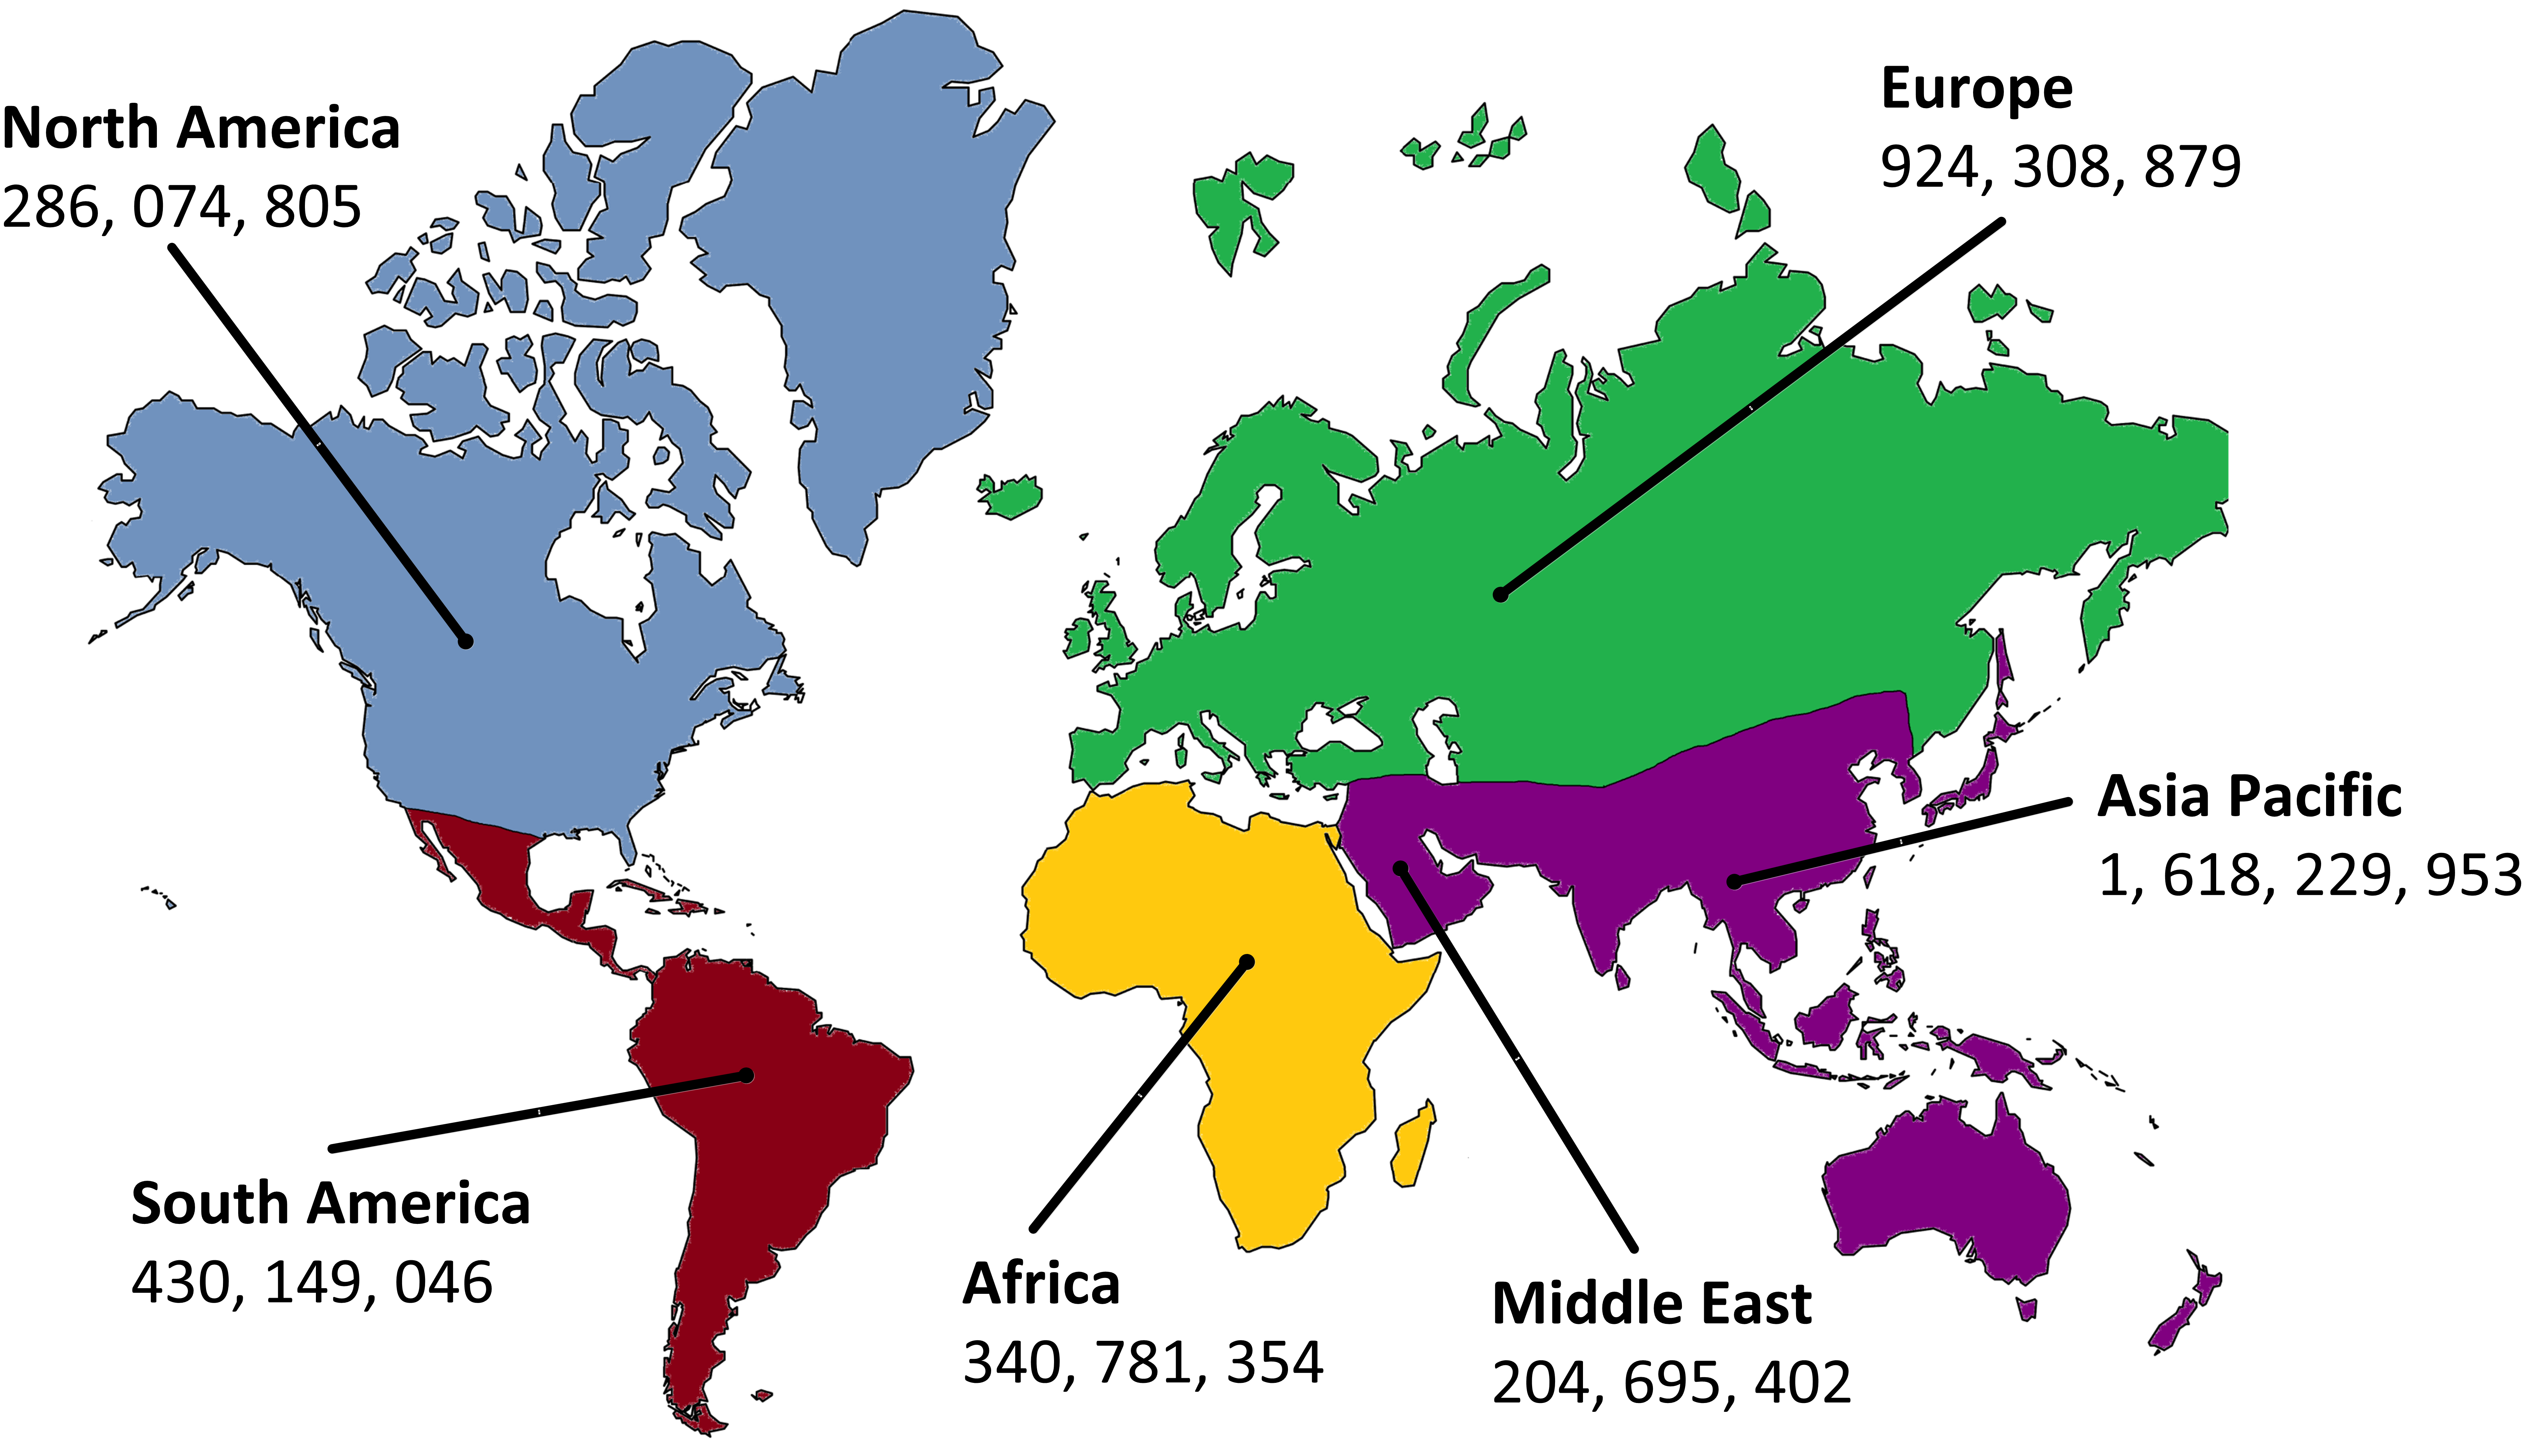
\includegraphics[width=0.8\textwidth]{chapter3/mobile_networks/subscriber_numbers.png}
  \caption{An indicator of the physical size of each region.}
  \label{fig:subscriberBase}
\end{figure}


Since the original mobile phone was first introduced in the 1980s, the 
underlying technology had gone through four major phases, known as generations 
\citep{cox08}.

The first generation of mobile phones (1G) utilised analogue communication 
techniques. These devices were famously bulky and expensive, and during the 
mid-1990s the second generation (2G) was introduction \citep{cox08}.

The second generation utilised the more powerful digital communication 
techniques, which allowed for the cost of the technology to reduce rapidly and 
for more services to be run. These additional services are now widely use and 
examples are text messaging, email and basic internet access \citep{cox08}.

Third generation (3G) and the newer fourth generation (4G) phones still utilise 
the digital communications spectrum. However the phones send and receive their 
signals in a different way from their predecessors, and from each other 
\citep{cox08}. 

For example 4G devices utilises a two antenna system, whereas the 3G only 
utilises one. The result of this is that the devices are able to support higher
data rates, which allows for video calls and high speed internet access.

A cellular system will be controlled by a particular operator (e.g. EE, O2 or 
Vodafone) and is referred to as a public land mobile network (PLMN). The PLMN 
has three aspects \citep{cox08}:
\begin{itemize}
  \item The Core Network
  \item The Radio Access Network
  \item The Mobile Phone
\end{itemize}

This is visualised within figure \ref{fig:mobileSystem} below.

\begin{figure}[H]
  \centering
    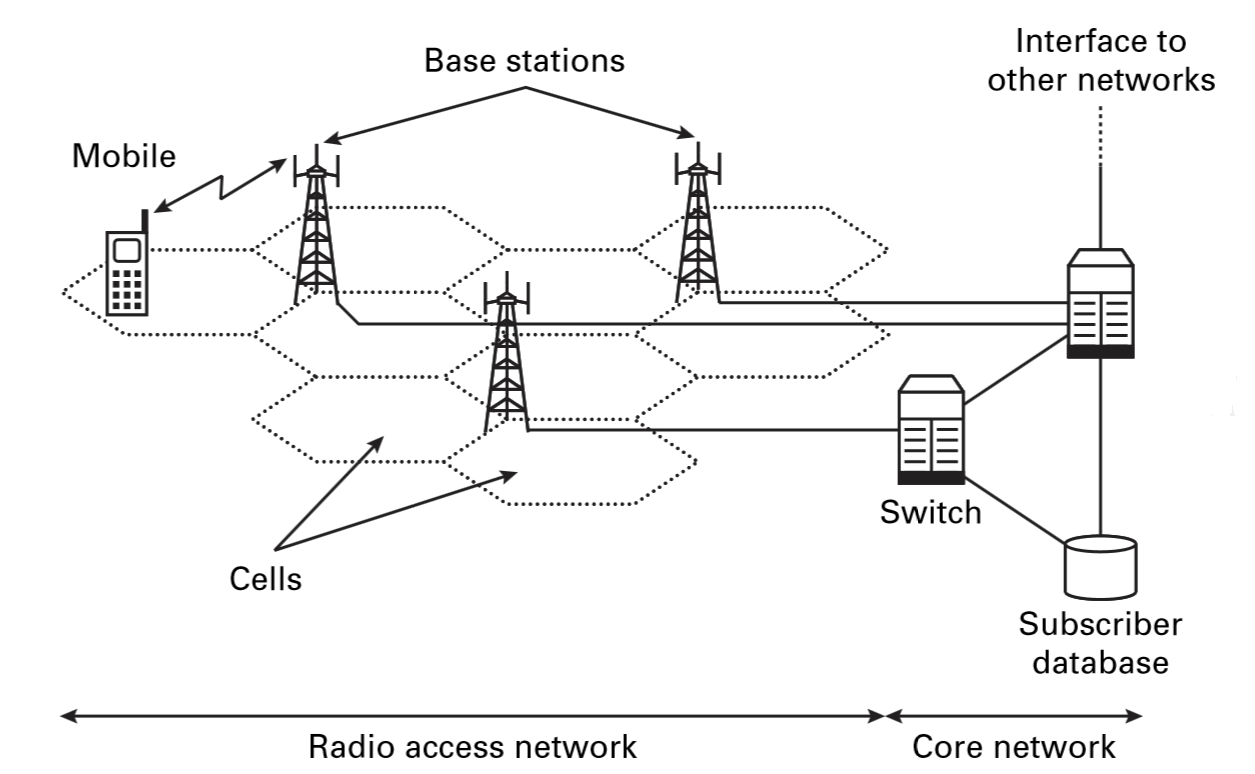
\includegraphics[width=0.8\textwidth]{chapter3/mobile_networks/mobile_architecture.png}
  \caption{The basic concept behind the mobile telecommunication system.}
    \label{fig:mobileSystem}
\end{figure}

The core network mimics a traditional fixed line telephone network. It's 
objective is to send voice calls or text messages from one phone to another 
using various switches. These switches could be thought as network switches 
found in computer networks \citep{cox08}.

The core network will also maintain a database containing information about the
network operator’s subscribers, as well as monitoring the locations of mobile 
phones. Monitoring each mobile phone's location, allows for an always-on style 
of connection to the mobile network, hence allowing calls to be made upon the
move \citep{cox08}.

The radio access network (RAN) ``handles the radio communications between the 
core network and the mobile phone'' \citep{cox08}. It contains a large number 
of base stations, each of which transmits and receives radio signals to and 
from the mobile phones in the surrounding area.

Each base station is equipped with multiple directional antennas \citep{cox08}, 
and will support one or more cells –-- usually three \citep{mpirical10}.

Each cell will have a maximum size –-- determinate by the largest distance that 
radio signals can be successfully sent and received \citep{cox08}. A radio wave
that interacts with objects (such as trees, buildings, hills, cars, people etc)
will have a huge impact upon coverage \citep{mpirical10}.

In order to gain the maximum radio coverage, radio planners will utilise various 
modelling and planning tools which are able to predict the likely coverage for 
a given area \citep{mpirical10}.

These tools allow for the minimisation of costs and maximisation of cell 
coverage, by determining the best location for each base station 
\citep{mpirical10}.

Figure \ref{fig:signalStrength} highlights the coverage area for a 2G base 
station. The base station is highlighted by a cross with a circle around it
\citep{mpirical10}.

\begin{figure}[H]
  \centering
    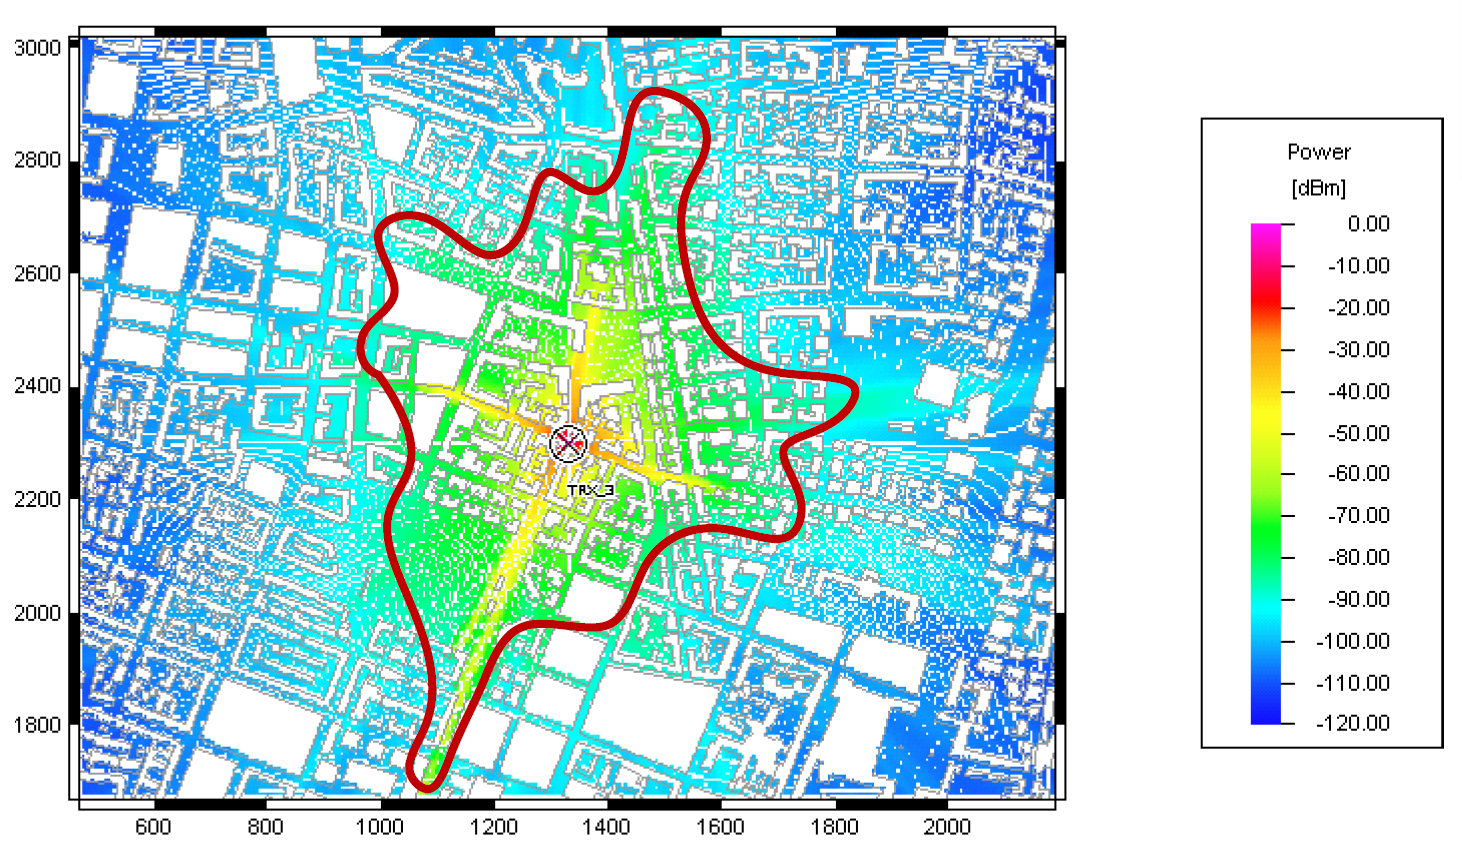
\includegraphics[width=0.8\textwidth]{chapter3/mobile_networks/mobile_network_intensity.png}
  \caption{An example output from a network modelling tool.}
  \label{fig:signalStrength}
\end{figure}

Figure \ref{fig:signalStrength} shows that some areas receive a stronger signal
than others, and as previously mentioned this is related to the number of 
objects within the areas that degrade the signal strength. To counter this 
mobile networks arrange cells upon a hierarchical structure \citep{mpirical10}. 
Each cell can be classified as either a:
\begin{itemize}
  \item Macro Cell
  \item Micro Cell
  \item Pico Cell
\end{itemize}

A Marco Cell is able to provide wide scale coverage. These cells are generally 
found within rural areas in which the usage would be deemed light. The radio 
antenna for a Macro Cell is usually found at the top of radio masks, to ensure 
the largest coverage possible \citep{mpirical10}.

A Micro Cell is able to provide street level coverage. These cells are 
generally found within urban areas and can be used in areas where coverage is 
high. The radio antenna for a Micro Cell is usually found upon the side of 
buildings or upon small street level masks \citep{mpirical10}.

A Pico Cell is able to provide room or building level of coverage. These cells 
are generally found within office or home spaces where the usage is extremely 
high. The radio antenna for a Pico Cell is usually found within one corner of 
a room or within the ceiling \citep{mpirical10}.

Figure \ref{fig:cellHierarchy} outlines the various different types of cells as 
a hierarchical diagram \citep{mpirical10}.

\begin{figure}[H]
  \centering
    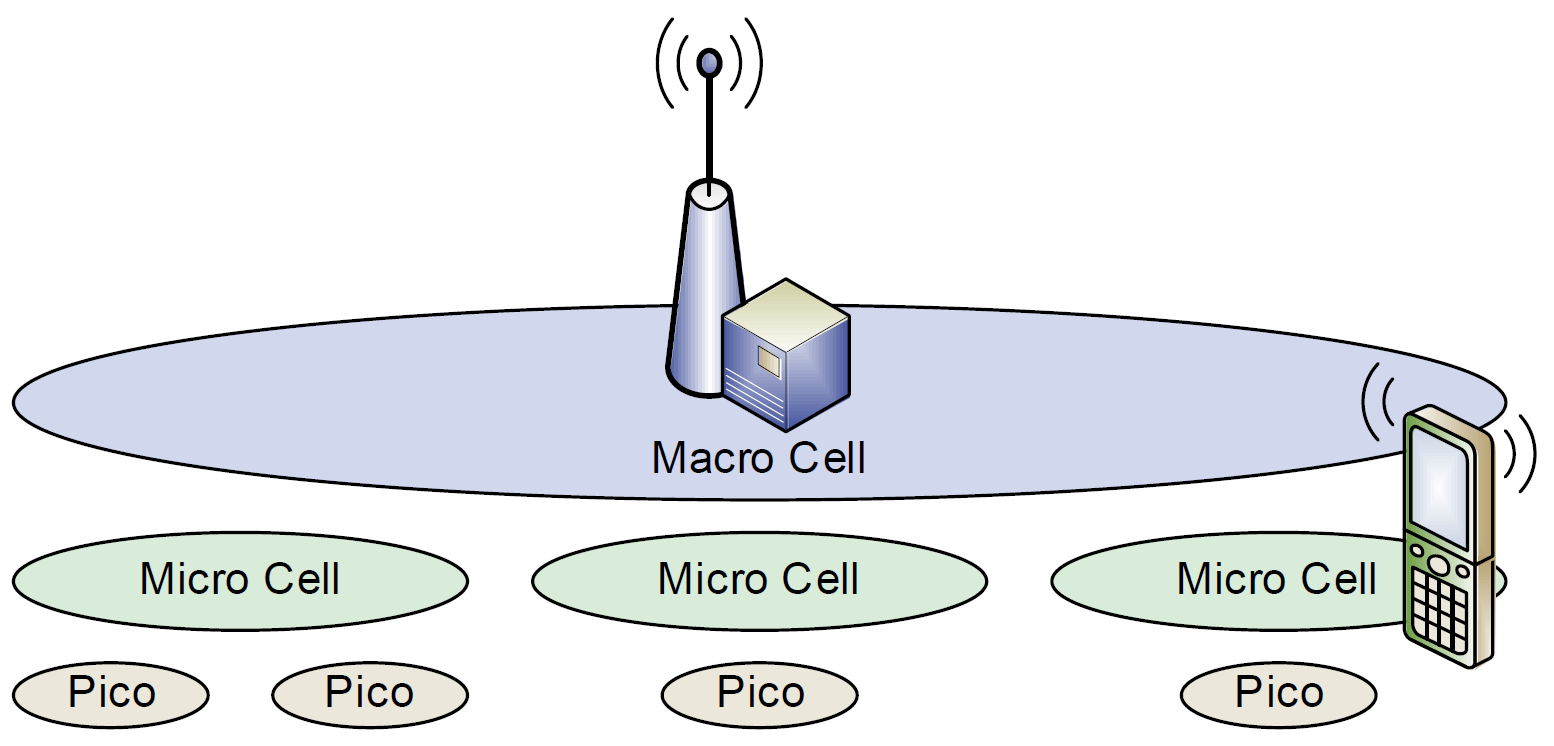
\includegraphics[width=0.80\textwidth]{chapter3/mobile_networks/network_hierarchy.png}
  \caption{Cell hierarchical structure.}.
  \label{fig:cellHierarchy}
\end{figure}

The main reason for using cells within the mobile system is that it allows for 
radio frequencies to be reused in difference locations. The reuse of frequencies 
simply allows for more mobile phones to be supported at any one given time 
\citep{cox08}. This setup also prevents any co-channel interface 
\citep{mpirical10}.

So far the term mobile phone has been used. However due to technological 
changes in recent years, mobile phones are not the only sole device that can 
access the mobile network. For example cellular dongles, tablet computers, 
cameras, e-readers and card readers are just a small number of devices that are 
able to use the cellular network. 

It is for this reason that the term user equipment (UE) is officially used 
within the Universal Mobile Telecommunications System (UMTS) specification 
instead of the term mobile phone \citep{cox08,mpirical10}. 

Throughout this project, the term device and UE will be used interchangeably. 


% Chapter 2 - Problem Analysis
\chapter{Problem Analysis}

In order ensure that this project remains focused, an initial problem analysis
has been undertaken. Within this chapter a selection of key areas and topics 
will be selected as a research topic. The problem analysis will also define the
problem in a much more detailed approach than what has been seen so far.

% Problem Environment
\newpage
\section{Defining the Environment}

BlackBerry test multiple devices within an automated test harness upon various 
weekly global drive routes. These routes are designed to test and stress the
device to the limits.

When a device encounters an event (good or bad), a call log is generated. A 
call log that can be deemed as a `Call Drop', `Setup Failure' or 
`Successful Call'. 

Each device will go on test for a number of hours (usually six hours), and 
during that time, the device will:
\begin{itemize}
  \item Make an automated call that is due to last for ninety seconds;
  \item Perform email bombs (sending and receiving thousand's of emails during 
        a short time --- usually thirty seconds);
  \item Wait for thirty seconds before making the next call (to allow for any 
        logging process to finish).
\end{itemize}

On average a call log is generated every one hundred seconds, and to avoid data 
implosion, only the `Call Drop' and `Setup Failure' logs will be analysed.

Each test device is paired to a reference device. A reference device is a device
that is currently deemed `stable', and is usually one that can be bought 
by consumers. Note: a test device is {\em usually} one that is currently in 
development, however it could be a competitor's device. 

% Problem Definition
\newpage
\section{Defining the Problem}
\label{sec:defining_the_problem}

Based upon the given environment, there are a number of comparisons that can be
made, however the main comparisons that this project will focus upon are:
\begin{itemize}
  \item Radio Access Technology (RAT);
  \item Frequency Mix-Bands;
  \item Radio Resource Controller (RRC).
\end{itemize}

Each of the above terminology will be expanded upon and defined within section 
\ref{sec:mobile_network_terminology}.

Fundamentally, the overall aim of this project is to `group' call logs into 
some form of comparable, well-defined categories.

By grouping the call logs from various devices and/or various different weeks,
test engineers are able to build a more solid picture of exactly the problems
that a device currently possess.

Once a problem has been identified, a number of solutions can then be proposed 
and ultimately can be implemented to fix the initial problem. It is the initial 
problem identification that this project and ultimately the product will focus 
upon.

% Research Areas
\newpage
\section{Research Areas}

Based upon the previous problem environment definition and the problem 
definition a larger survey was able to be conducted.

\subsection{Initial Survey}
An initial survey was originally conducted which would try to determine the 
research paths that should be taken. The survey should also try to determine if
the problem has already been solved before.

Unfortunately due to the vast secrecy of the mobile computing industry it was
unclear whether or not this problem has already been solved before. 

This was mainly down to the fact that device manufacturers do not release key
performance indicators about their devices upon particular networks, as this 
information is particularly damaging to the device manufacturers and the mobile
networks operators.

However it is highly unlikely that the objects that have been set by client are
the same objectives as any previous or current system. 

Even though there is no evidence to suggest that there is (or isn't) a similar 
tool already available, the problem can sill be solved with standard computing 
practices.

\subsection{Clustering}
The problem definition (section \ref{sec:defining_the_problem}) described the 
solution to the outlined problems as ``grouping the call logs''. In order to 
gain valid, comparable groupings a standardised methodology should be used. 
This field of computing is known as cluster analysis, and is part of the larger 
data mining sub-field.

As each route is fixed it is possible to compare various weeks' testing to 
other weeks. However it must be noted that this project will only focus upon 
clustering the `Call Drop' and `Setup Failure' call logs. The reason for this 
is that successful calls do not provide much analysis, in comparison to a 
failed call.

\subsection{Visualisation}
The problem definition also mentions the fact that once the `grouping of data' 
is completed, some form of visual representation of the groupings is required. 
Data Visualisation is concerned with trying to obtain information from a set 
of data. 

As cluster analysis forms sets of `similar' data, it would certainly seem 
logical at this stage to ensure that both clustering and data visualisation 
techniques are covered.

\subsection{The Mobile Network}
The basics of the mobile network should also be researched. This will allow all
readers of this project to gain an understanding of some of the technical 
terminologies associated with this project.

In summary, the following areas will be researched into further to help gain a
more vivid understanding the problem at large.

\begin{itemize}
  \item Mobile Network
  \item Clustering Algorithms
  \item Visualisation of Data
\end{itemize}


% Chapter 3 - Research
\chapter{Research}

% Introduction to the Mobile Network
\newpage
\section{Mobile Networks}

\subsection{Introduction to the Mobile Network}
In 2010, it was estimated that the total global mobile phone subscriber base 
exceeded 3.8 billion users \citep{mpirical10}. These figures can be categorised 
into the following geographical areas, as show in figure \ref{fig:subscriberBase} 
below.

\begin{figure}[H]
  \centering
    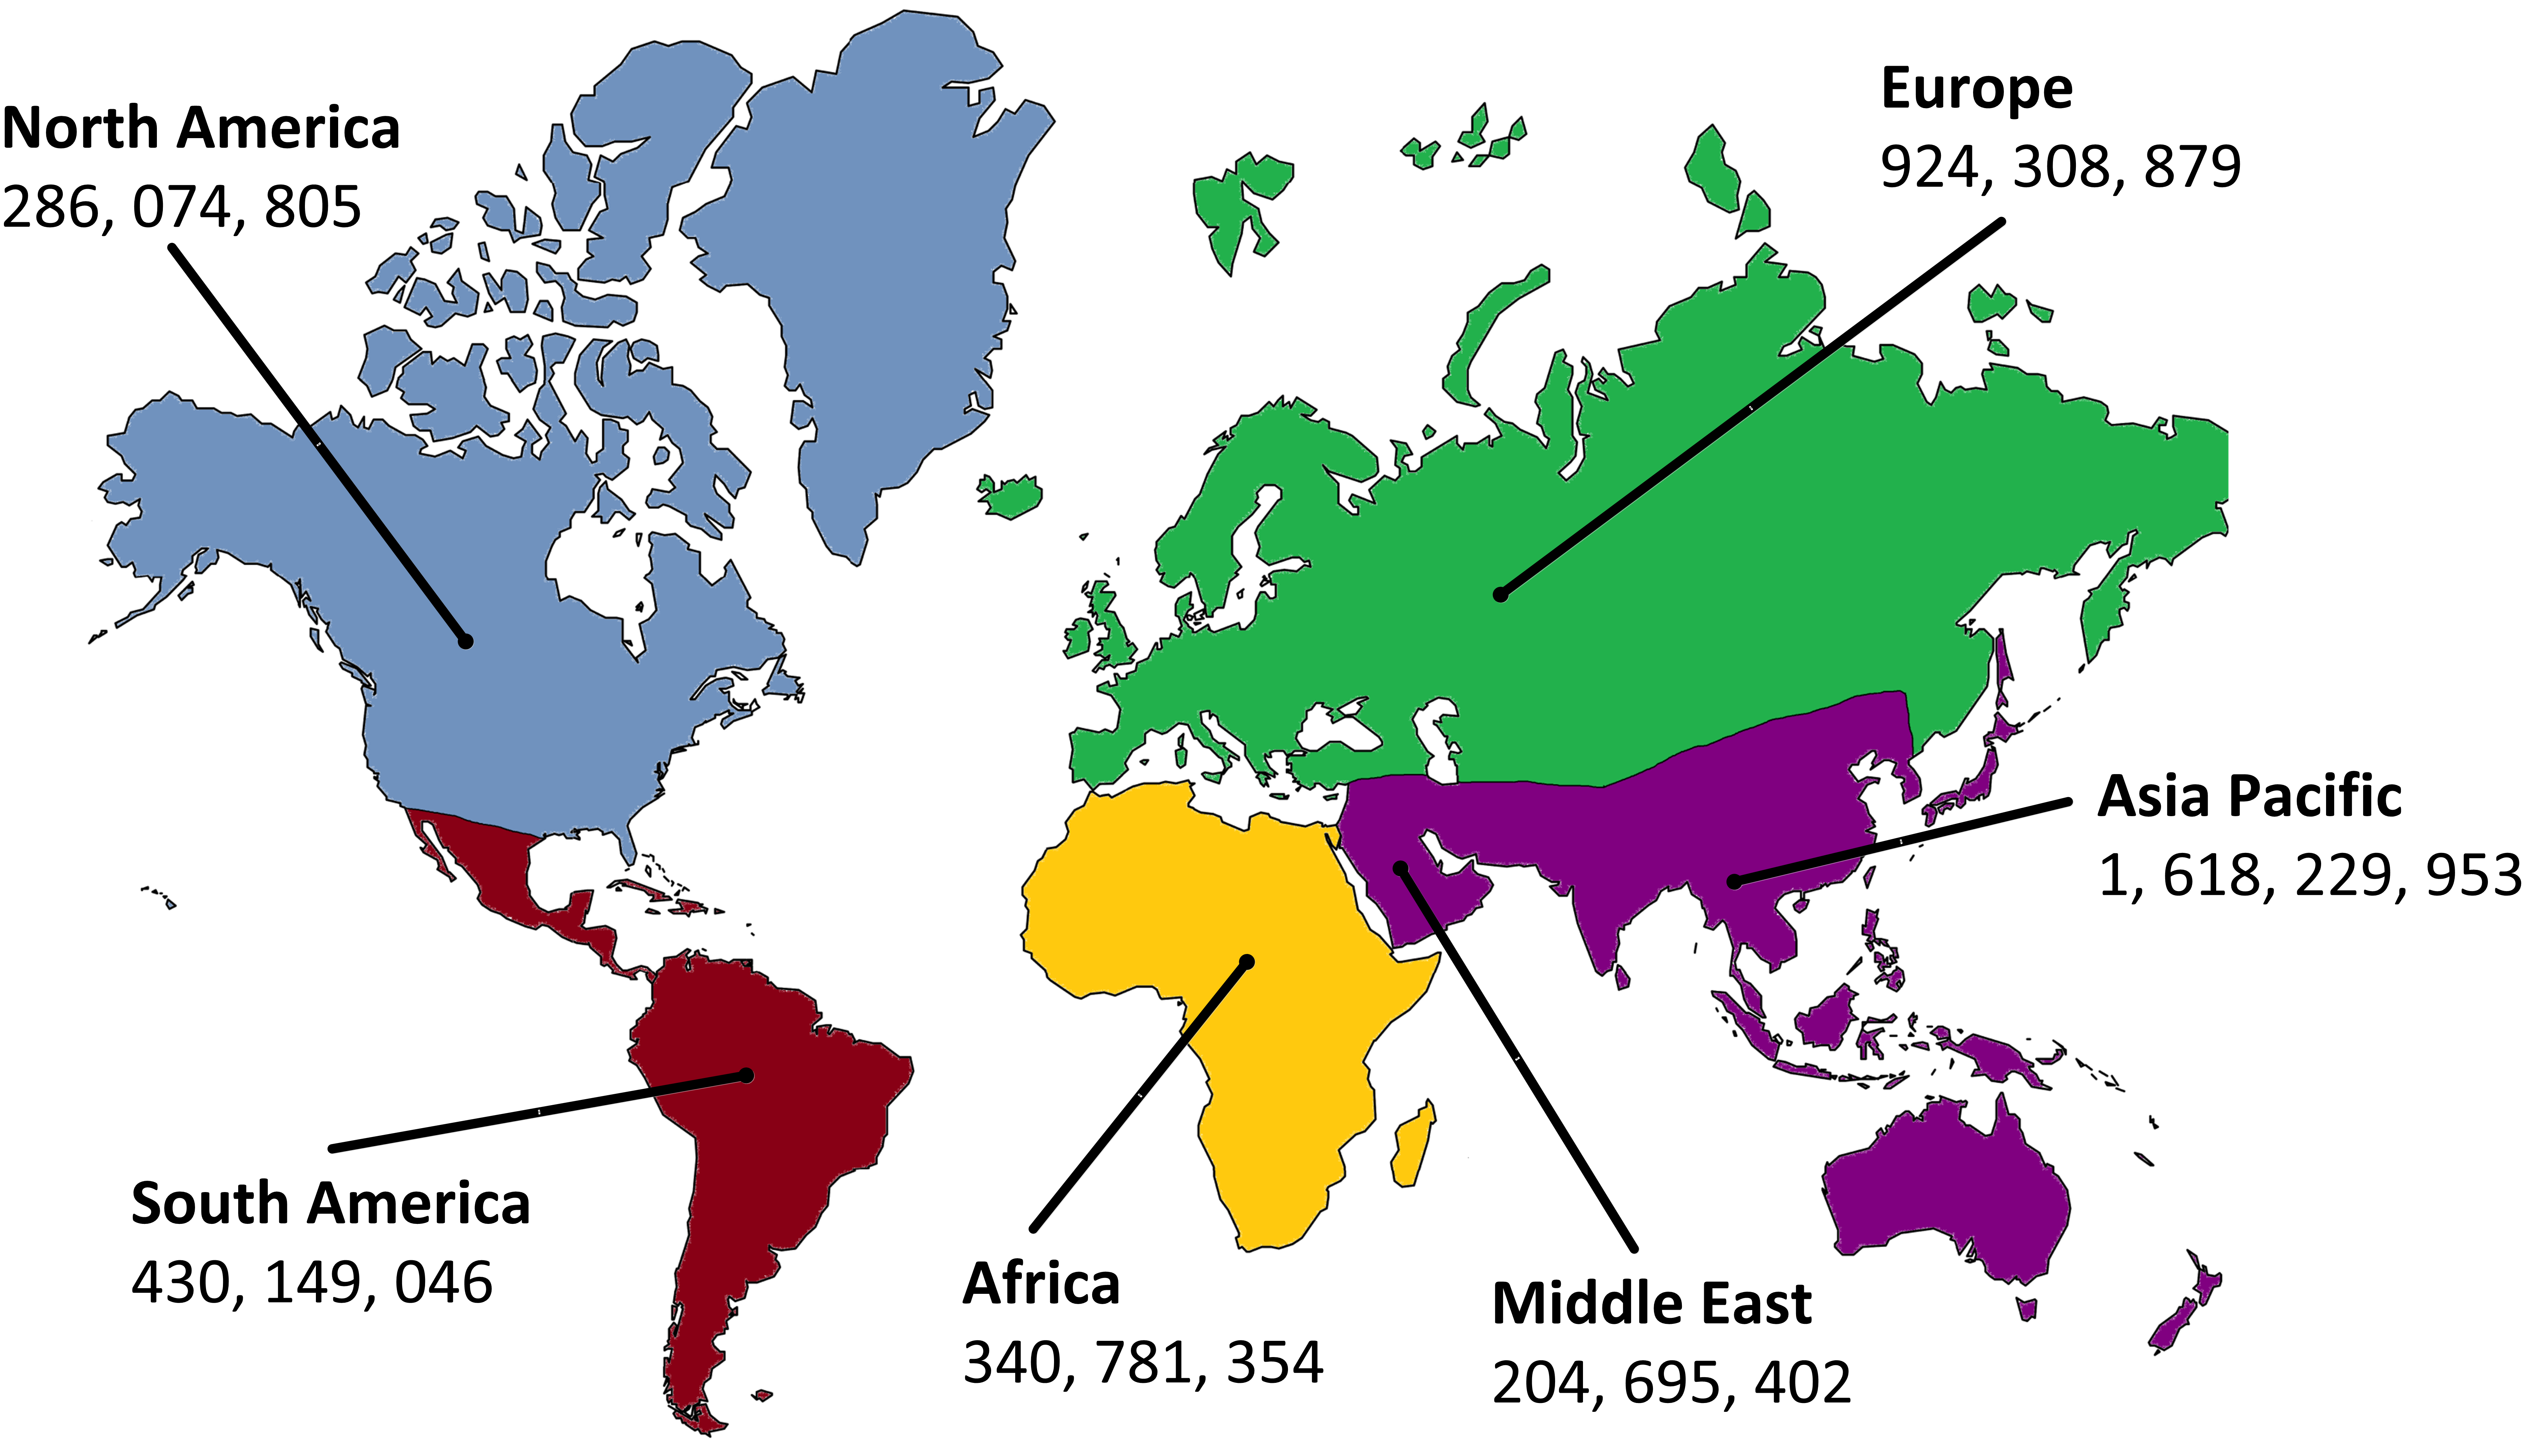
\includegraphics[width=0.8\textwidth]{chapter3/mobile_networks/subscriber_numbers.png}
  \caption{An indicator of the physical size of each region.}
  \label{fig:subscriberBase}
\end{figure}


Since the original mobile phone was first introduced in the 1980s, the 
underlying technology had gone through four major phases, known as generations 
\citep{cox08}.

The first generation of mobile phones (1G) utilised analogue communication 
techniques. These devices were famously bulky and expensive, and during the 
mid-1990s the second generation (2G) was introduction \citep{cox08}.

The second generation utilised the more powerful digital communication 
techniques, which allowed for the cost of the technology to reduce rapidly and 
for more services to be run. These additional services are now widely use and 
examples are text messaging, email and basic internet access \citep{cox08}.

Third generation (3G) and the newer fourth generation (4G) phones still utilise 
the digital communications spectrum. However the phones send and receive their 
signals in a different way from their predecessors, and from each other 
\citep{cox08}. 

For example 4G devices utilises a two antenna system, whereas the 3G only 
utilises one. The result of this is that the devices are able to support higher
data rates, which allows for video calls and high speed internet access.

A cellular system will be controlled by a particular operator (e.g. EE, O2 or 
Vodafone) and is referred to as a public land mobile network (PLMN). The PLMN 
has three aspects \citep{cox08}:
\begin{itemize}
  \item The Core Network
  \item The Radio Access Network
  \item The Mobile Phone
\end{itemize}

This is visualised within figure \ref{fig:mobileSystem} below.

\begin{figure}[H]
  \centering
    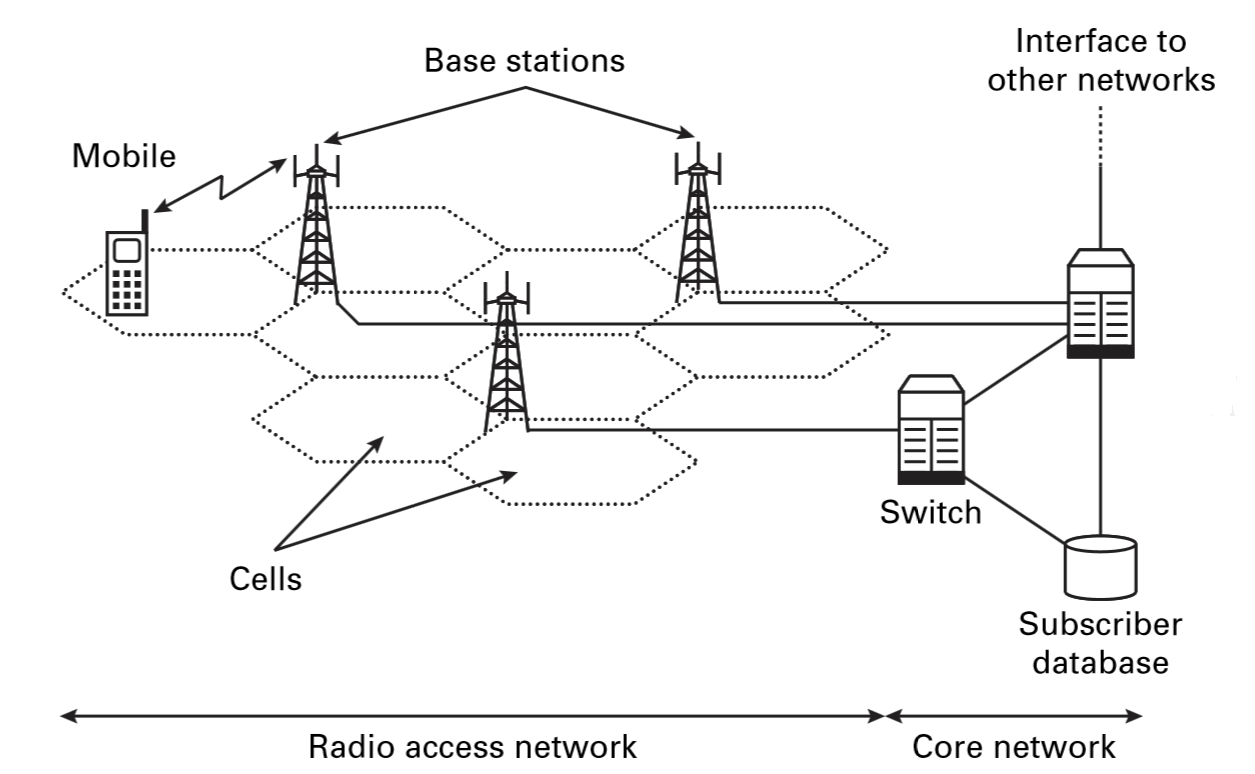
\includegraphics[width=0.8\textwidth]{chapter3/mobile_networks/mobile_architecture.png}
  \caption{The basic concept behind the mobile telecommunication system.}
    \label{fig:mobileSystem}
\end{figure}

The core network mimics a traditional fixed line telephone network. It's 
objective is to send voice calls or text messages from one phone to another 
using various switches. These switches could be thought as network switches 
found in computer networks \citep{cox08}.

The core network will also maintain a database containing information about the
network operator’s subscribers, as well as monitoring the locations of mobile 
phones. Monitoring each mobile phone's location, allows for an always-on style 
of connection to the mobile network, hence allowing calls to be made upon the
move \citep{cox08}.

The radio access network (RAN) ``handles the radio communications between the 
core network and the mobile phone'' \citep{cox08}. It contains a large number 
of base stations, each of which transmits and receives radio signals to and 
from the mobile phones in the surrounding area.

Each base station is equipped with multiple directional antennas \citep{cox08}, 
and will support one or more cells –-- usually three \citep{mpirical10}.

Each cell will have a maximum size –-- determinate by the largest distance that 
radio signals can be successfully sent and received \citep{cox08}. A radio wave
that interacts with objects (such as trees, buildings, hills, cars, people etc)
will have a huge impact upon coverage \citep{mpirical10}.

In order to gain the maximum radio coverage, radio planners will utilise various 
modelling and planning tools which are able to predict the likely coverage for 
a given area \citep{mpirical10}.

These tools allow for the minimisation of costs and maximisation of cell 
coverage, by determining the best location for each base station 
\citep{mpirical10}.

Figure \ref{fig:signalStrength} highlights the coverage area for a 2G base 
station. The base station is highlighted by a cross with a circle around it
\citep{mpirical10}.

\begin{figure}[H]
  \centering
    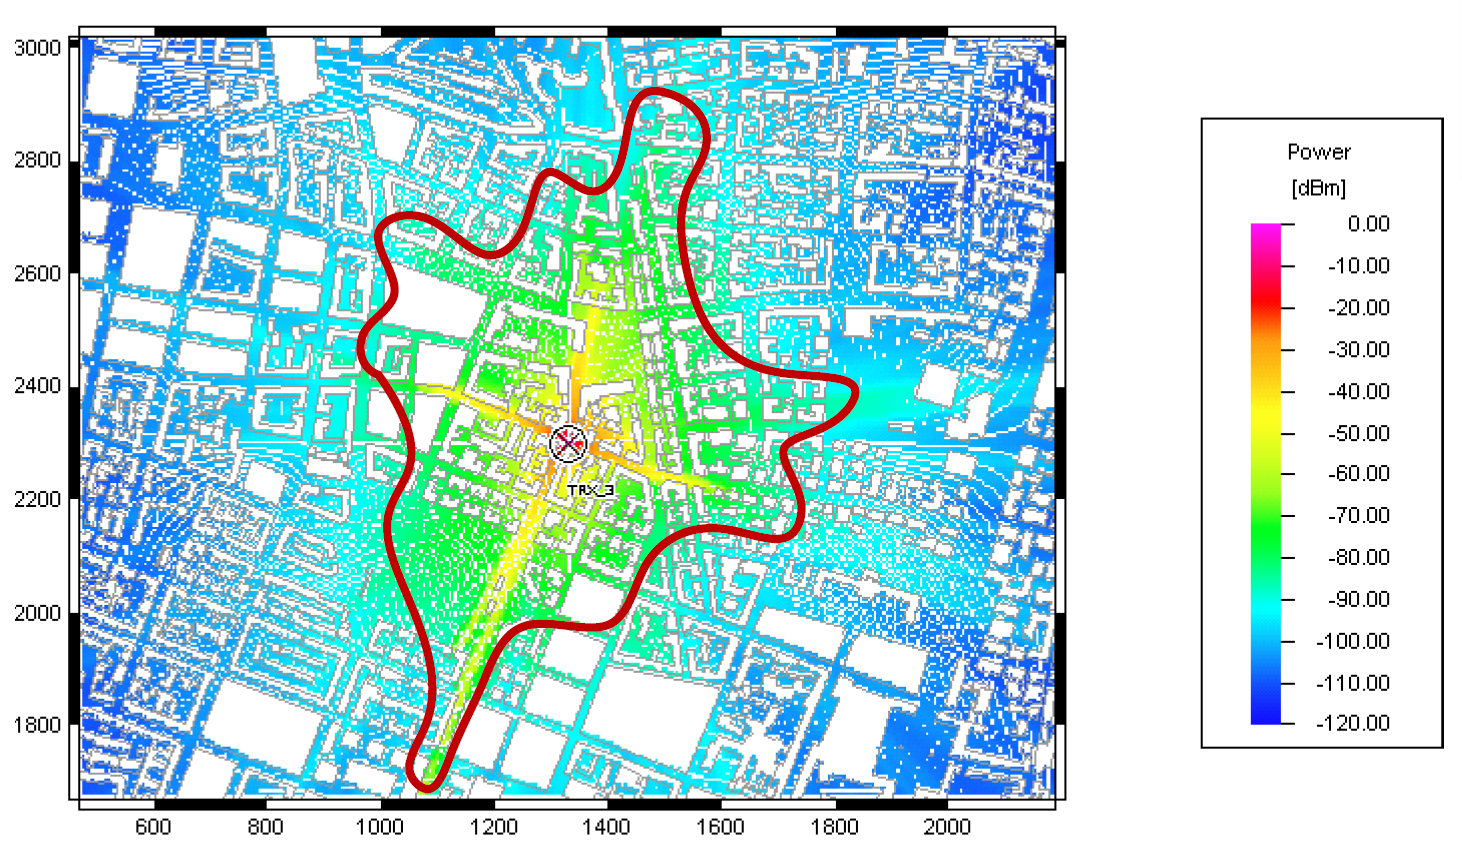
\includegraphics[width=0.8\textwidth]{chapter3/mobile_networks/mobile_network_intensity.png}
  \caption{An example output from a network modelling tool.}
  \label{fig:signalStrength}
\end{figure}

Figure \ref{fig:signalStrength} shows that some areas receive a stronger signal
than others, and as previously mentioned this is related to the number of 
objects within the areas that degrade the signal strength. To counter this 
mobile networks arrange cells upon a hierarchical structure \citep{mpirical10}. 
Each cell can be classified as either a:
\begin{itemize}
  \item Macro Cell
  \item Micro Cell
  \item Pico Cell
\end{itemize}

A Marco Cell is able to provide wide scale coverage. These cells are generally 
found within rural areas in which the usage would be deemed light. The radio 
antenna for a Macro Cell is usually found at the top of radio masks, to ensure 
the largest coverage possible \citep{mpirical10}.

A Micro Cell is able to provide street level coverage. These cells are 
generally found within urban areas and can be used in areas where coverage is 
high. The radio antenna for a Micro Cell is usually found upon the side of 
buildings or upon small street level masks \citep{mpirical10}.

A Pico Cell is able to provide room or building level of coverage. These cells 
are generally found within office or home spaces where the usage is extremely 
high. The radio antenna for a Pico Cell is usually found within one corner of 
a room or within the ceiling \citep{mpirical10}.

Figure \ref{fig:cellHierarchy} outlines the various different types of cells as 
a hierarchical diagram \citep{mpirical10}.

\begin{figure}[H]
  \centering
    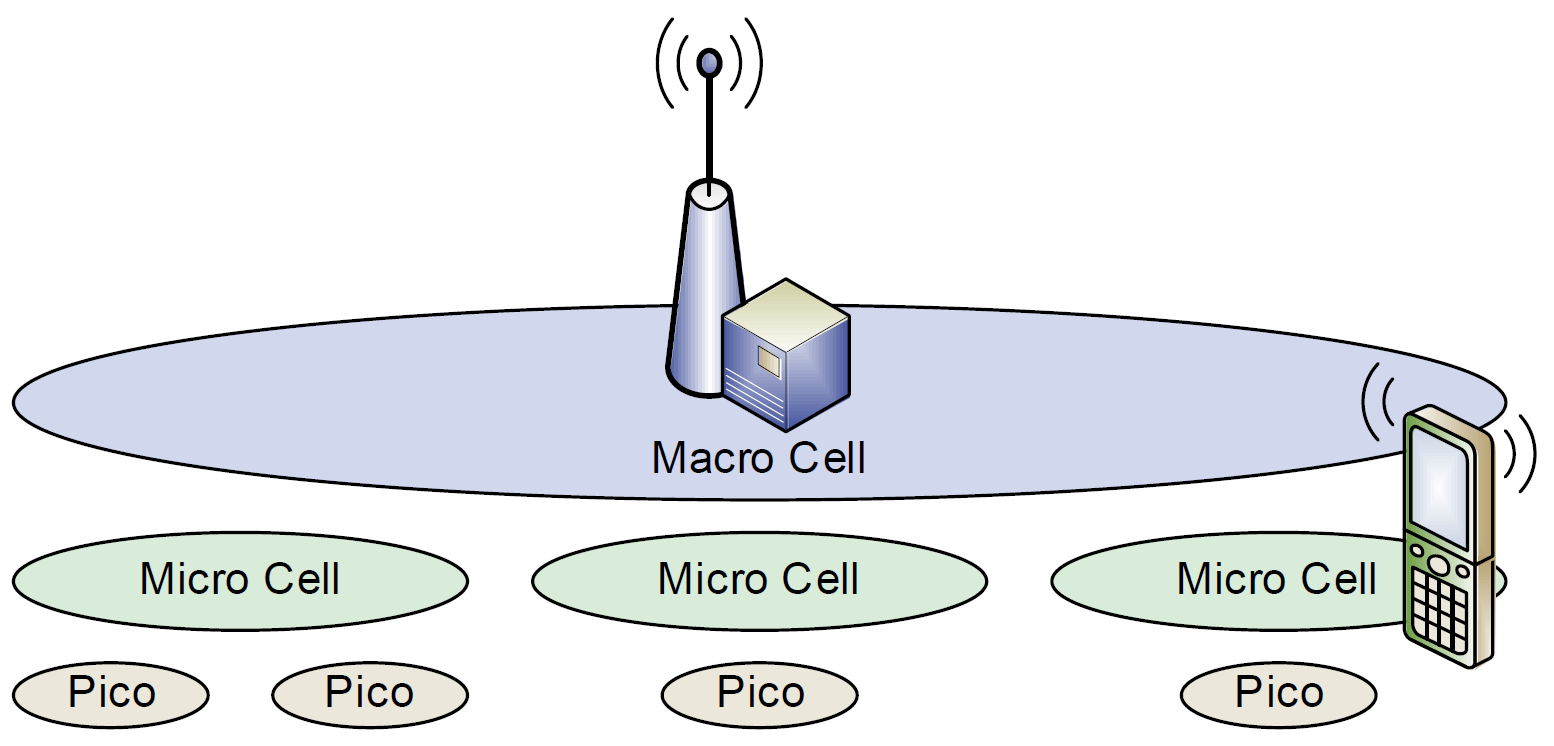
\includegraphics[width=0.80\textwidth]{chapter3/mobile_networks/network_hierarchy.png}
  \caption{Cell hierarchical structure.}.
  \label{fig:cellHierarchy}
\end{figure}

The main reason for using cells within the mobile system is that it allows for 
radio frequencies to be reused in difference locations. The reuse of frequencies 
simply allows for more mobile phones to be supported at any one given time 
\citep{cox08}. This setup also prevents any co-channel interface 
\citep{mpirical10}.

So far the term mobile phone has been used. However due to technological 
changes in recent years, mobile phones are not the only sole device that can 
access the mobile network. For example cellular dongles, tablet computers, 
cameras, e-readers and card readers are just a small number of devices that are 
able to use the cellular network. 

It is for this reason that the term user equipment (UE) is officially used 
within the Universal Mobile Telecommunications System (UMTS) specification 
instead of the term mobile phone \citep{cox08,mpirical10}. 

Throughout this project, the term device and UE will be used interchangeably. 


\subsection{Mobile Network Terminology}
\label{sec:mobile_network_terminology}
A number of terminologies will now be defined and described in order to aid 
further understanding of the project.

\subsubsection{Radio Access Technology}
The Radio Access Technology (RAT) refers to the method in which a given device 
connects to the core network. Examples are:
\begin{itemize}
  \item UTRA (UMTS Terrestrial Radio Access), known simply as 3G
  \item GERAN (GSM EDGE Radio Access Network), known simply as 2G
\end{itemize}

The core network routes traffic through various switches. Each RAT will have 
it's own ``dedicated network''. It is possible however to handover from one 
network to another.

Within this project, these will be referred to by the terms ``Start RAT'' and 
``End RAT''. A section of possible RAT combinations are shown below:
\begin{multicols}{3}
  \begin{itemize}
    \item 2G $\Rightarrow$ 2G
    \item 2G $\Rightarrow$ 3G
    \item 2G $\Rightarrow$ 4G
    \item 3G $\Rightarrow$ 2G
    \item 3G $\Rightarrow$ 3G
    \item 3G $\Rightarrow$ 4G
    \item 4G $\Rightarrow$ 2G
    \item 4G $\Rightarrow$ 3G
    \item 4G $\Rightarrow$ 4G
  \end{itemize}
\end{multicols}

The RAT upon the left hand side of the separator is the Start RAT and the RAT 
upon the right hand side of the separator is the End RAT. So for the given 
example:

\begin{quote}
  2G $\Rightarrow$ 3G
\end{quote}

it would read:

\begin{quote}
  ``The given UE had a Start RAT of 2G and an End RAT of 3G''
\end{quote}


\subsubsection{Frequency}
In order to allow multiple UEs to operate upon the same RAT different 
operator frequencies have to be used \citep{cox08}. However to ensure that 
frequencies are efficiently distrusted, frequencies will be reused by following
a ``frequency reuse plan''. 

This prevents situations where by the some frequencies ``come together'', which
ultimately results in co-channel interference \citep{mpirical10}.

Figure \ref{fig:frequencyReuse} highlights a repeat pattern, in this instance 
a four cell repeat pattern. ``The most important fact about cell planning is 
the reuse distance as this determines when it is possible to reuse the same 
frequency'' \citep{mpirical10}.

\begin{figure}[H]
  \centering
    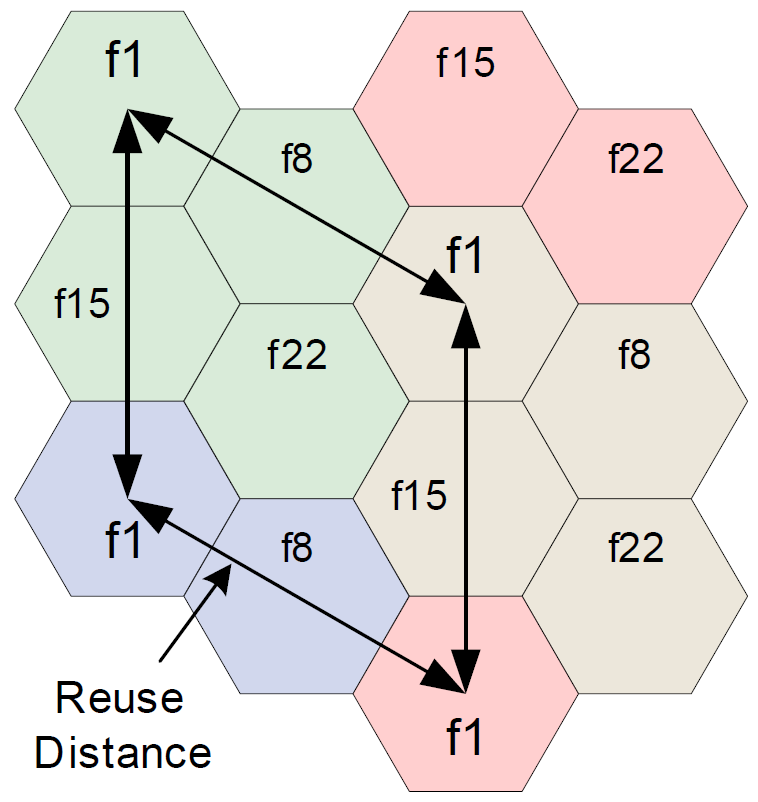
\includegraphics[width=0.4\textwidth]{chapter3/mobile_networks/frequency_reuse.png}
  \caption{An example frequency reuse plan.}.
  \label{fig:frequencyReuse}
\end{figure}

In this example there is always one cell between co-channels, and hence this 
would reduce the interference between the same channels. However it must also 
be mentioned that radio waves do not simply stop at the edge of a cell. 

Signals will ``propagate for many more kilometres'' \citep{mpirical10}. However
because of the reuse distance, the carrier signal --- the wanted signal --- 
should be far more powerful than the interferer signal --- the unwanted signal 
from neighbouring cells --- \citep{mpirical10} .

Within this project the frequency will be referred to as the Mix-Band. This is 
because the Mix-Band refers to 2G, 3G and 4G frequencies and not simply one 
type of frequency. 

Each frequency will comprise of a ``Start Mix-Band'' and an ``End Mix-Band''. 
An example selection of possible Mix-Band combinations are shown below (note 
there could be many hundred):

\begin{multicols}{3}
  \begin{itemize}
    \item GSM 900 $\Rightarrow$ GSM 900
    \item GSM 900 $\Rightarrow$ DCS PCS
    \item GSM 900 $\Rightarrow$ 10763
    \item DCS PCS $\Rightarrow$ GSM 900
    \item DCS PCS $\Rightarrow$ DCS PCS
    \item DCS PCS $\Rightarrow$ 10763
    \item 10763 $\Rightarrow$ GSM 900
    \item 10763 $\Rightarrow$ DCS PCS
    \item 10763 $\Rightarrow$ 10763
  \end{itemize}
\end{multicols}


\subsubsection{Radio Resource Control}
The Radio Resource Control (RRC) is found within layer three (the network 
layer) of the OSI Seven Layer Model. The RRC is the routing manager, and will 
contain various routing options that are stored in a routing table. 
The routing table is similar to those found in routers, however it also 
performs other functions such as establishing and releasing connections 
\citep{mpirical10}.

The RRC has a state, and can be one of the following:
\begin{itemize}
  \item CELL DCH (Dedicated Channel)
  \item CELL FACH (Forward access channel)
  \item CELL PCH (Cell Paging channel) 
  \item URA PCH (URA Paging channel)
  \item IDLE (No Connection)
\end{itemize}


The CELL DCH state has a dedicated, physical channel allocated to the device. 
This gives the device the ability to perform uplink and downlinks (of data and 
calls). The device's location is updated constantly \citep{umtsworld}.

CELL DCH mode is relatively expensive (both upon the device's battery 
consumption and the network power) this mode is only used for making and 
receiving calls \citep{umtsworld}.

Whereas the CELL FACH state has no dedicated physical channel (virtual channel) 
allocated to the device. The device will be allowed to monitor the downlink but
is unable to make uplink calls from this state. The device's location is 
updated regularly \citep{umtsworld}.

CELL PCH is the same as CELL FACH (no dedicated physical channel), however the 
longitude and latitude of the device is updated only when moving between cells 
\citep{umtsworld}. 

If a UE was to use the internet usage, it would more than likely `sit' in CELL 
PCH mode, unless {\bf heavy} internet usage was in progress. The reason being
is that the device does not need a dedicated connection --- the ``packets'' 
could come in any order, where as a telephone conversation would not work if 
the end of the conversation came before the start.

URA PCH state is simply used for monitoring purposes. No uplink activity is 
possible \citep{umtsworld}.

The difference between a dedicated (physical channel) and a non-dedicated 
(virtual channel) is somewhat simlar to that found in TCP vs UDP. Like TCP, a
dedicated channel ensures that ``packets'' are send and received in order, 
where as a non-dedicated channel may see the ``packets'' received in the wrong 
order, or not even at all!

Although all four states are independent of each other, it is possible for a 
device to ``step up'' or ``step down'' between states. For example if a call is
about to be made or received, then that UE would need to request the highest 
amount of `power' from the network. The UE would ``step up'' to the CELL DCH 
mode.

A graphical representation of the power consumption by each state is shown 
in the ``theoretical graph'' below.

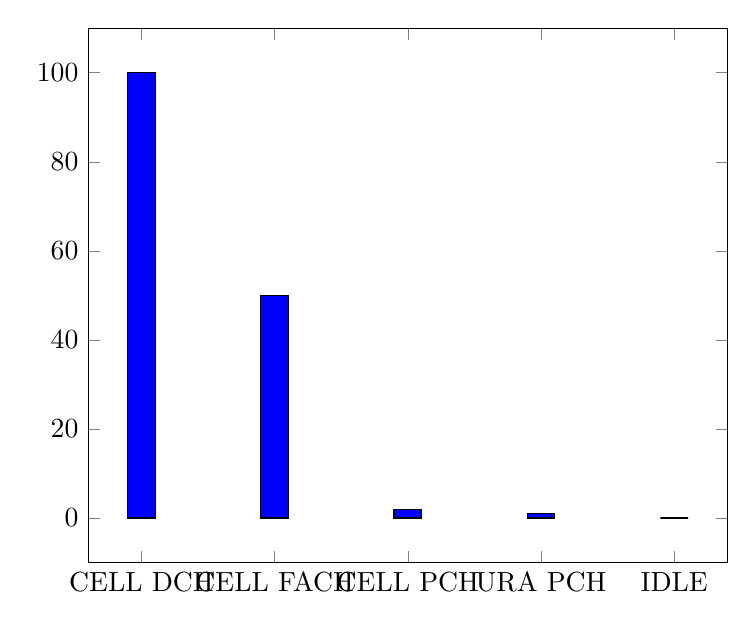
\begin{tikzpicture}
  \begin{axis}[
      width=0.80\textwidth,
      symbolic x coords={CELL DCH, CELL FACH, CELL PCH, URA PCH, IDLE},
      xtick=data
    ]
    \addplot[ybar,fill=blue] coordinates {
        (CELL DCH,   100)
        (CELL FACH,  50)
        (CELL PCH,   2)
        (URA PCH,    1)
        (IDLE,       0)
    };
  \end{axis}
  \label{graph:rrcPower}
\end{tikzpicture}

The graph above utilises ``theoretical'' values, however the percentages of 
these values are deemed to be correct. 

CELL DCH uses as much power as it can get, so in this example this is set to 
100\%. Devices that are in the CELL FACH state will only use around 50\% of the
power that the CELL DCH state would use, and CELL PCH would only use around 
2\%. URA PCH (if supported) would use 1\% of the CELL DCH state with IDLE 
utilising 0\% \citep{umtsworld}.

The RRC State selection is made at a mobile operator level. This means that one 
operator may choose to use all five states, where by another operator may only 
choose to use three. The different configurations and states leads to 
differences in energy consumption \citep{umtsworld}.

Unlike the previous terms, the RRC state will stay fixed throughout the 
duration of some activity (whether that be a call or data transfer). This 
project refers to the RRC state as the Start RRC state.


% Clustering Algorithms Research
\newpage
\section{Clustering Algorithms}

\subsection{What is Clustering}
Clustering is the process of grouping a set of objects into classes of similar 
objects that are meaningful, useful or both \citep{tan05}.

A cluster is a collection of objects that are similar (or related) to one 
another within that same cluster and are dissimilar (or unrelated) to other 
objects within other clusters. The more distinct the similarity within a group, 
and the greater difference between groups, the more distinct the final clustering 
will be \citep{han06}.

Cluster analysis can be found in many areas, even fundamentally in the 
development of humans. From a young age, we learn how to distinguish between 
different types of animals, such as cats and dogs \citep{han06}. 

We have been able to do this by continuously clustering the data objects. Every
time we discovered a new attribute of that object, we would subconsciously 
improve our clustering schemes \citep{han06}. 

Cluster analysis is actively used in various industries, such as social sciences, 
biology, statistics, machine learning, data analysis, market research and pattern 
recognition \citep{han06}.

Cluster analysis has been used within a biological environment for many years. 
It can be used to categorise genes with similar (or dissimilar) functionality, 
and gains insights into structures that are inherent within certain groups of 
populations \citep{han06}.

Clustering can also be used for outlier detection. An outlier is a value that 
is a large distance from any given cluster. These outliers can be of more 
interest than the actual clusters \citep{tan05}. 

Fraud monitoring systems will try to find exceptional credit card transactions 
(such as highly expensive or frequent purchases) by clustering the common 
(or ``accepted'') purchases together. This would then allow better 
identification of the unexpected purchases \citep{tan05}.

The defining of a cluster is the most important, and yet the hardest part of 
any application. Figure \ref{fig:clusterDefinition} shows twenty points, and 
three different ways of separating them into clusters, in which each cluster 
membership is deduced by its colour.

\begin{figure}[H]
  \begin{center}
    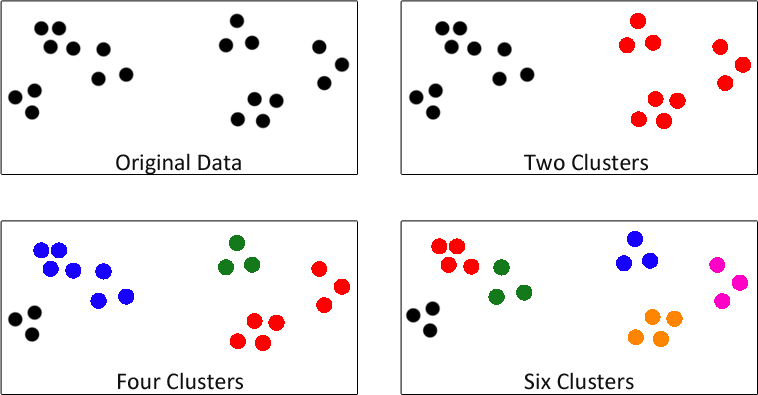
\includegraphics[width=0.80\textwidth]{chapter3/clustering/ClusterDefinition1.png}
    \label{fig:clusterDefinition}
    \caption
      {Different ways of clustering the same set of points.}
  \end{center}
\end{figure}

We can easily separate the original points into two clusters; however on closer 
inspection it appears that the two clusters have further clusters inside them. 
This figure illustrates the important fact that the definition of a cluster is 
imprecise. The definition of a cluster is not only specific to the nature of the 
data but the required results as well.

\subsection{Clustering Methods}
There are many clustering algorithms, and despite this it is quite difficult to 
provide a well-defined categorisation of these clustering methods, because many
of categories overlap each other \citep{everitt74}.
For the purposes of this project, the following five categories will be used:
\begin{itemize}
  \item Partitioning
  \item Hierarchical
  \item Density-based
  \item Grid-based
  \item Model-based
\end{itemize}


\subsection{Partitioning Methods}
A partitioning algorithm will organise {\emph n} number objects within a 
dataset, into {\emph k} non-overlapping partitions (clusters) as long as 
{\emph k} $\leq$ {\emph n} \citep{han06}. 

This means that each object will belong to one cluster and one cluster only. 

The objects in a cluster are more similar with each other, in comparison to 
objects that belong to other clusters. These are regarded as being dissimilar 
in terms of the data set attributes \citep{tan05}.

\subsubsection{K-Means}
The K-Means algorithm will partition a set of objects into {\emph k} number of 
clusters in such a way that the similarity of the objects that make up a 
cluster is high, but the similarity of two or more separate clusters (and their 
objects) is low.

Cluster similarity is measured with regards to the average (mean) value of all 
objects in a given cluster. This average value is known as the cluster's 
centroid.

The K-Means algorithm will firstly randomly select {\em k} number of objects 
from the dataset and put them into their own cluster \citep{han06}. For each of
the remaining objects in the dataset, an object is assigned to the cluster that
it is most similar to \citep{tan05}.

The similarity is based upon the distance between the object in question and 
the centroid object of a given cluster. Once the pass is completed, the 
centroid of all clusters is recomputed to gain the new mean cluster 
\citep{tan05}. 

This process will continue to run until there have been no object moves 
detected \citep{han06}.

\paragraph*{K-Means Formal Algorithm}
\subparagraph*{Input:}
\begin{itemize}
  \item {\bf K} - the number of clusters
  \item {\bf D} - the data set of {\em n} objects
\end{itemize}

\subparagraph*{Output:}
\begin{itemize}
  \item A set of k clusters {\em K}
\end{itemize}

\subparagraph*{Method:}
\begin{enumerate}
  \item randomly choose k objects from D;
  \item {\bf repeat}
  \item \begin{list}{$\square$}{\leftmargin=1em \itemindent=0em}
          assign each object to the cluster to which it is most similar to the 
          cluster’s centroid;
        \end{list}
  \item \begin{list}{$\square$}{\leftmargin=1em \itemindent=0em}
          update the cluster centroid for each cluster;
        \end{list}
  \item {\bf until} no change;
\end{enumerate}

Computationally speaking, the K-Means algorithm maybe faster than hierarchical 
clustering methods, if the number of cluster, {\emph k}, is small \citep*{ios}.
The reason for this is that the algorithm utilises the centroid as a 
comparative object. 

The algorithm can also produce more tightly packed clusters in comparison to 
hierarchical based clustering \citep{ios}.

However comparing the accuracy of the clusters that have been produced can be 
difficult, especially as the number of clusters, k, affects the outcome. In order 
to improve the accuracy of the results, it may be required to run the algorithm 
several times with different k value (\citep{ios}).

\subsubsection{K-Medoids}
One of the main issues faced with the K-Means algorithm, is that it is highly 
sensitive to outliers, because the centroid object is the mean of all the 
objects within that cluster \citep{tan05}. It is possible to modify the K-Means
algorithms to remove such sensitivity \citep{tan05}. 

Instead of creating a mean centroid object based upon all the objects within 
that cluster, we could pick an actual object to represent the centroid. Each 
remaining object would then be clustered with the centroid object that is it 
most similar to \citep{tan05}.

The algorithm would iterate until each centroid is actually the medoid of its 
cluster. It is this idea that forms the basis of the K-Medoids algorithm for 
grouping a set of objects into {\em k} clusters \citep{everitt74}.

The initial centroid objects are chosen at random According to \citep{tan05}. 
The process of replacing the current centroid with another object continues as 
long as the resulting clustering is improved \citep{tan05}. 

The quality of the clustering is measured using a cost method, which will 
measure the average dissimilarity between an object and the centroid of the 
cluster \citep{tan05}.

\paragraph*{K-Medoids Formal Algorithm}
\subparagraph*{Input:}
\begin{itemize}
  \item {\bf K} - the number of clusters
  \item {\bf D} - the data set of {\em n} objects
\end{itemize}

\subparagraph*{Output:}
\begin{itemize}
  \item A set of k clusters {\em K}
\end{itemize}

\subparagraph*{Method:}
\begin{enumerate}
  \item 1.  randomly choose {\em k} objects from D as the initial centroids;
  \item {\bf repeat}
  \item \begin{list}{$\square$}{\leftmargin=1em \itemindent=0em}
          assign each remaining object to the cluster to the nearest cluster, 
          based upon the centroids;
        \end{list}
  \item \begin{list}{$\square$}{\leftmargin=1em \itemindent=0em}
          randomly choose a non-centroid object, {\em o};
        \end{list}
  \item \begin{list}{$\square$}{\leftmargin=1em \itemindent=0em}
          compute the total cost of swapping the centroid object with, {\em o};
        \end{list}
  \item \begin{list}{$\square$}{\leftmargin=1em \itemindent=0em}
          if total cost $<$ 0 then swap the centroid with {\em o};
        \end{list}
  \item {\bf until} no change;
\end{enumerate}


The K-Medoids proves to be a robust algorithm in the presence of noise and/or 
outliers. The reason for this is because the medoid is not influenced by extreme 
values, as found with the mean value.

The algorithm is efficient for small sets of data, but can be inefficient in 
terms of time when working with large data sets.


\subsection{Hierarchical Methods}
If clusters were ``allowed'' to have sub clusters, then we would then 
automatically obtain a hierarchical clustering method \citep{tan05}. This 
clustering method simply groups objects into a tree of clusters. The root node 
of the tree contains all clusters, with each node (cluster) in the tree the 
union of its children.

There are two branches of hierarchical clustering, agglomerative and divisive. 
The only difference between the two is the direction in which clustering 
happens \citep{tan05}.

The agglomerative algorithm utilises a bottom-up (merging) strategy, whereas 
the divisive algorithm utilises a top-down (separating) strategy \citep{tan05}. 
Figure \ref{fig:hierarchicalDefinition} shows the two forms of hierarchical 
clustering side by side. 

\begin{figure}[H]
  \centering
  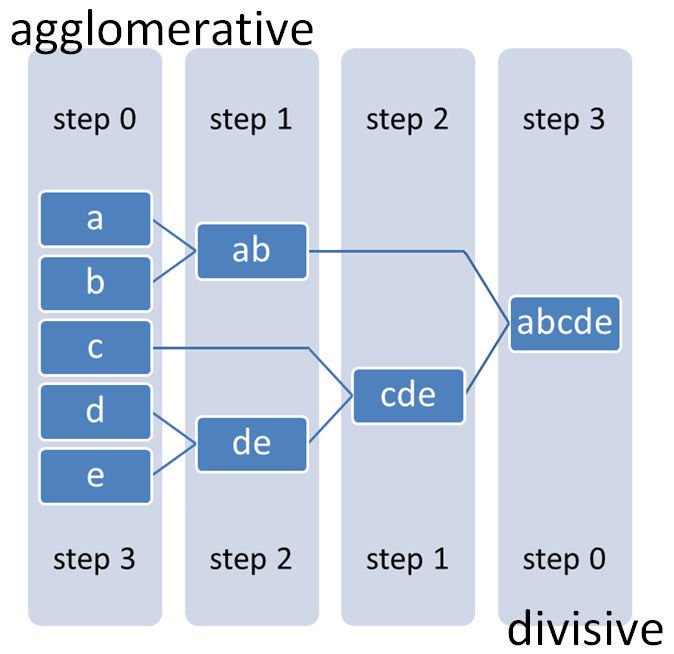
\includegraphics[width=0.7\linewidth]{chapter3/clustering/hierarchical.png}
  \label{fig:hierarchicalDefinition}
  \caption
   {Two main methods of clustering hierarchically.}
\end{figure}

The agglomerative method initially places each object into a cluster of its own, 
and the clusters are then merged according to some criterion, such as Euclidean 
distance \citep{tan05}. 

The process of merging clusters to form larger embedded clusters continues 
until one cluster is formed. The last cluster could be thought of as the `root 
cluster' \citep{han06}.

In contrast, the divisive method will place all objects into one initial cluster. 
The algorithm will then split this cluster into child clusters based upon a 
criterion \citep{tan05}. 

The criterion could be anything, but as with the agglomerative method the 
Euclidean distance between the closest neighbouring objects in the cluster is 
a popular criterion. The splitting process continues until each new cluster 
only contains a single object \citep{han06}.

One of the key elements to hierarchical clustering is the computation of the 
proximity between two clusters --- proximity matrix --- \citep{tan05}. It is 
this definition that will change with each variation of the algorithms. 

There are three methods to calculate the proximity between two clusters
\citep{tan05}. These are outlined below:

\begin{itemize} 
  \item \textbf{Single Link} (MIN) defines the cluster proximity as the 
        proximity between the closest two objects within two different 
        clusters. 
        \begin{figure}[H]
          \centering
          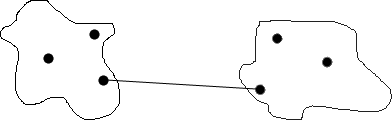
\includegraphics[width=0.60\linewidth]{chapter3/clustering/min.png}
        \end{figure}

  \item \textbf{Complete Link} (MAX) defines the cluster proximity as the 
        proximity between two farthest objects within two different clusters.
        \begin{figure}[H]
          \centering
          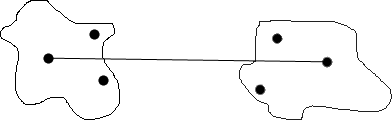
\includegraphics[width=0.60\linewidth]{chapter3/clustering/max.png}
        \end{figure}

  \item \textbf{Group Average} defines the cluster proximity as the average 
        pairwise proximities of all pairs of objects from two different 
        clusters.
        \begin{figure}[H]
          \centering
          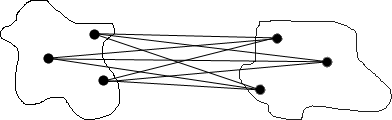
\includegraphics[width=0.60\linewidth]{chapter3/clustering/group_average.png}
        \end{figure}
\end{itemize}


\subsubsection{Agglomerative}
The agglomerative algorithm is a bottom-up strategy, and hence all objects are 
placed into their own cluster \citep{tan05}. The algorithm will then merge the 
two closest pair of clusters, and will continue doing this in order to create 
larger and larger clusters. 

The end point of the algorithm is reached when all of the objects are in a 
single cluster. Each specific implementation of the agglomerative algorithm 
is the same, differing only in the definition of inter-cluster similarity 
\citep{tan05}.

\paragraph*{Agglomerative Formal Algorithm}
\subparagraph*{Input:}
\begin{itemize}
  \item {\bf D} - the data set of {\em n} objects
\end{itemize}

\subparagraph*{Output:}
\begin{itemize}
  \item A set of clusters
\end{itemize}

\subparagraph*{Method:}
\begin{enumerate}
  \item Compute the proximity matrix (may not be required);
  \item {\bf repeat}
  \item \begin{list}{$\square$}{\leftmargin=1em \itemindent=0em}
          Merge the closest two clusters;
        \end{list}
  \item \begin{list}{$\square$}{\leftmargin=1em \itemindent=0em}
          Update the proximity matrix for both the new and original clusters;
        \end{list}
  \item {\bf until one} cluster remains.
\end{enumerate}

Agglomerative algorithms produce an ordering of the objects 
\citep{iosHierarchical}, which can be advantageous for data display, where the 
ordering of the data might be important. 

Agglomerative algorithms also have a tenancy to produce smaller clusters, which
can be helpful for knowledge discovery \citep{iosHierarchical}.

The agglomerative algorithm is unable to perform an adjustment (undo) once the 
merge process has been completed. This means that if a chosen merge turns out 
to be unsound, the method is unable to backtrack, and an entire re-run of the 
algorithm would be required \citep{tan05}. 

\subsubsection{Divisive}
The divisive algorithm is a top-down strategy \citep{han06}. All the objects 
are initially placed into one cluster. At each step, a cluster will be split, 
and this will be repeated until each cluster has exactly one cluster 
\citep{tan05}. 

The main decision of this algorithm is to correctly decide which cluster to 
split up at each stage, and how exactly do to the splitting. As with the 
agglomerative algorithm, the specific implementation of the divisive algorithm 
is the same, differing only in the definition of inter-cluster similarity 
\citep{tan05}.

\paragraph*{Divisive Formal Algorithm}
\subparagraph*{Input:}
\begin{itemize}
  \item {\bf D} - the data set of {\em n} objects
\end{itemize}

\subparagraph*{Output:}
\begin{itemize}
  \item A set of clusters
\end{itemize}

\subparagraph*{Method:}
\begin{enumerate}
  \item 1.  Place all objects into one cluster;
  \item {\bf repeat}
  \item \begin{list}{$\square$}{\leftmargin=1em \itemindent=0em}
          Find the object which has the highest average dissimilarity in 
          comparison to the other objects. Place this object into a new 
          cluster, C;
        \end{list}
  \item \begin{list}{$\square$}{\leftmargin=1em \itemindent=0em}
          {\bf repeat}
        \end{list}   
  \item \begin{list}{$\square$}{\leftmargin=1em \itemindent=0em}
          \begin{list}{$\square$}{\leftmargin=1em \itemindent=0em}
            For each object X not in C, compute the distance;
          \end{list}  
        \end{list}        
  \item \begin{list}{$\square$}{\leftmargin=1em \itemindent=0em}
          \begin{list}{$\square$}{\leftmargin=1em \itemindent=0em}
            If the distance $>$ 0, then merge the object X to C
          \end{list}  
        \end{list}   
  \item \begin{list}{$\square$}{\leftmargin=1em \itemindent=0em}
          {\bf until} all the distances calculated are negative;
        \end{list} 
  \item \begin{list}{$\square$}{\leftmargin=1em \itemindent=0em}
          Choose the cluster with the largest dissimilarity between any of its 
          two objects, and divide this cluster;
        \end{list} 
  \item {\bf until all} clusters contain one object;
\end{enumerate}

As with the agglomerative algorithm, the divisive algorithm produces an ordering
of the objects, which can be advantageous for data display. Smaller clusters 
are generally generated, which can be helpful for knowledge discovery 
\citep{iosHierarchical}.

As with the agglomerative algorithm, the divisive algorithm is unable to 
perform an adjustments (undo) once the split process has been completed. An 
entire re-run of the algorithm would be required, if a chosen split turned out
to be unsound \citep{tan05}.


\subsection{Density-Based Methods}
Density-based algorithms try to locate regions that are of high density and 
separate these regions from the data space \citep{tan05,han06}. Regions that 
are of a low density are either ignored, or removed completely from the data 
space \citep{han06}.

Unlike the previous algorithms discussed, clusters can be of any arbitrary 
size, as a cluster is defined as dense regions of objects (rather than 
similarity between two objects).

\subsubsection{Density-Based Spatial Clustering of Applications with Noise}
\label{sec:DBSCAN}
The DBSCAN algorithm is a centre-based, density-based algorithm. The algorithm
is able to identify regions of high density into clusters, of any arbitrary 
shape \citep{han06}.

Density is estimated for a given object by counting the number of objects 
within the neighbourhood of a radius, {\em Eps} \citep{tan05}. A cluster is 
defined as a maximal set of density-connected objects. 

In order to fully define the DBSCAN algorithm, additional terms will be 
required to be defined. These terms are specific to the DBSCAN algorithm, and 
are listed below.

\begin{itemize}
  \item A core object is an object that falls within the {\em Eps} of a given 
        radius and when grouped with other points, the total number of points 
        exceeds the minimum points \citep{han06}.
  \item A border object is an object that falls within the neighbourhood of a 
        core object. A border object can fall in the neighbourhoods of more than 
        more core object. A border object is not a core object \citep{han06}.
  \item A noise object is any object that is not classified as either a core 
        object or as a border object \citep{han06}.
  \item The neighbourhood within a radius, {\em r}, of a given object is called 
        the r-neighbourhood of the object \citep{tan05}.
  \item An object is referred to as a core object if the r-neighbourhood of that 
        object contains at least a minimum number of objects \citep{tan05}.
  \item Object x is directly density-reachable from object y if object x is 
        within the r-neighbourhood of object y and object y is a core object
        \citep{tan05}.
\end{itemize}

The DBSCAN algorithm classifies an object as being:
\begin{enumerate}
  \item within a dense region (core object); {\bf \em or}
  \item on the edge of a dense region (border object); {\bf \em or}
  \item in a sparsely occupied region (noise object).
\end{enumerate}

Informally, the DBSCAN algorithm could be described as any two core objects 
that are within a distance, {\emph Eps}, of each other are placed into the same 
cluster. A border object that is close enough to a core object is placed into 
that cluster, with all noise objects being discarded. 

\paragraph*{DBSCAN Formal Algorithm}
\subparagraph*{Input:}
\begin{itemize}
  \item {\bf D} - the data set of {\em n} objects
\end{itemize}

\subparagraph*{Output:}
\begin{itemize}
  \item A set of clusters
\end{itemize}

\subparagraph*{Method:}
\begin{enumerate}
  \item Label all objects as core, border or noise objects within D;
  \item Remove the noise objects from D;
  \item Calculate the distance between all core objects that are within 
        {\em Eps} of each other;
  \item Make each group of connected core objects into their own cluster;
  \item Assign each border object to the closest core object’s cluster.
\end{enumerate}

One of the fundamentals of the DBSCAN algorithm is the notion of density 
reachability. It is because of this that the algorithm is able to automatically
detect clusters of objects, rather than having to specify the number of 
clusters --- unlike the partitioning methods --- \citep{han06}. 

If an object is unable to be placed into a cluster, it is classed as noise, thus 
improving the overall quality of the clusters.

The single-link effect (which is common in partitioning methods) is reduced 
dramatically \citep{tan05}, due to the inclusion of the minimum points value; 
this ultimately allows the algorithm to find clusters of any arbitrary shape
\citep{han06}. 

However the minimum points value is fixed at the start of the clustering 
process, and can cause problems with datasets that have large differences in 
densities \citep{han06}.

The algorithm is (generally) insensitive to the ordering of the objects in the
dataset. However if an object is sitting on the edge of two clusters, the 
membership to either cluster may change \citep{han06,tan05}.

Finally, the quality of the clusters depends upon the distance measuring 
method. The Euclidean distance calculation is normally used. This is based upon
Pythagoras' theorem, and utilises an ``as-the-crow-flies'' approach to finding
the distance between two points.

\subsection{Grid-Based Methods}
Grid-based algorithms utilise a multi-resolution grid structure. The algorithm 
will limit the object space into a set number of cells that forms a grid. It is 
upon this grid that all of the clustering operations are performed 
\citep{han06}.

The grid is generally a multi-dimensional structure, and therefore is not 
really applicable to clustering coordinates.

\subsection{Model-Based Methods}
Model-based algorithms attempt to place a mathematical model over a set of data. 
This is generally based upon the assumption that data are generated by using 
various probability distributions \citep{han06}.

As with the grid-based methods, these methods are not applicable to this 
project.


% Visualisation Research
\newpage
\section{Visualisation}
The final implementation stage was the visualisation of the results. To ensure 
that the visualisation was not tightly coupled to the analysis process, the 
visualisation aspect had been specifically kept as a separate entity.

The reason for this is that it allows BlackBerry to develop their own 
visualisation techniques if required, without having to change the main 
analysis processes.

\subsection{Data Management}
To ensure that the visualisation is loosely coupled with the analysis part of 
the tool, a simple data structure was required to be implemented.

As the charts were to be developed using web technologies (such as HTML, CSS 
and JavaScript), it made sense to maintain the data structures in JavaScript 
Object Notation (JSON), which is what the tool outputs.

\subsection{Charts}
In order to produce some visualisation charts, a JavaScript charting library is
required. The decision to use a well established charting library, rather than 
developing one from scratch was suggested by BlackBerry.

The requirement to develop visualisation charts was only identified as a 
`could' requirement (see section \ref{sec:could}). However due to time 
resourcing being managed well, this requirement could be fulfilled.

The charting library that was selected is call d3js. D3js is a ``JavaScript 
library for manipulating documents based on data'' \citep{d3js}. One of the 
major advantages for using d3js is that it is based upon open, standard web 
technologies (HTML, DOM, CSS and JavaScript).

This effectively means that the resulting output will be able to be displayed 
on almost any computer, without the requirement for additional software to be
installed --- other than a web standard browser.

Five charting techniques were selected to output the data, and are described in
more detail in the following subsections.


\subsubsection{Bar Chart}
The Bar Chart is one of the main points of entry to analyse the results. The 
raw data is arranged in a hierarchical structure, and this is something that 
the Bar Chart supports.

Figure \ref{fig:bar_chart_1} highlights an example bar chart from an initial 
point of view.

A user is able to ``drill down'' into the data to find specific information, by
simply clicking upon a given bar. Figure \ref{fig:bar_chart_2} highlights all 
the clusters whereby the 9800 device dropped calls upon a specific RAT. 

Clicking upon one of the bars again will drill down into the specifics of a 
cluster.

% Landscape page
\begin{landscape}
  % Center image
  \centering 
    \begin{figure}[H]
      \centering
        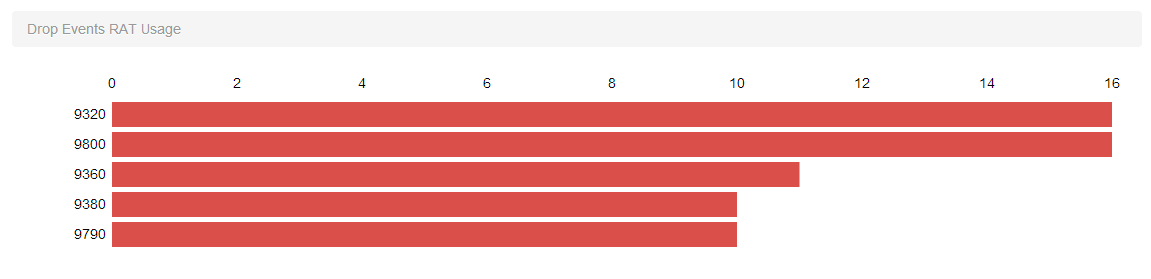
\includegraphics[scale=0.75]{chapter8/visualisation/bar_chart_1.png}
        \caption[Example Bar Chart output]
                {An Example Bar Chart output from the root node, highlighting all 
                 the various devices and their performance from a general point of 
                 view}
        \label{fig:bar_chart_1}
    \end{figure}
    ~\\
    \begin{figure}[H]
      \centering
        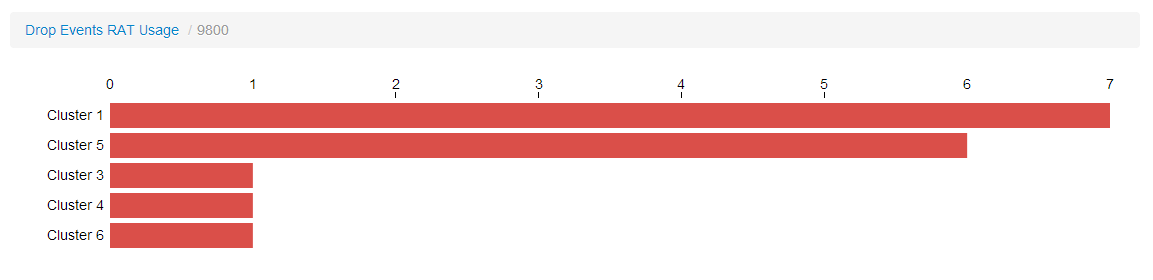
\includegraphics[scale=0.75]{chapter8/visualisation/bar_chart_2.png}
        \caption[Example Bar Chart output one node deep]
                {Example Bar Chart output one node deep --- i.e. all data that is
                 related to the 9800 device only.}
        \label{fig:bar_chart_2}
    \end{figure}
\end{landscape}


\newpage
\subsubsection{Circle Pack}
A Circle Pack diagram represents hierarchy through the use of embedded nodes. 
A Circle Pack diagram can be compared to a treemap, as it shares similar 
features however it is not as space-efficient. 

On the other hand it does reveal the overall size of each element (cluster, 
device, week, usage) more vividly in comparison to a treemap. Figure 
\ref{fig:circle_pack} illustrates an example output.

% Landscape page
\begin{landscape}
  % Center image
  \centering 
    \begin{figure}[H]
      \centering
        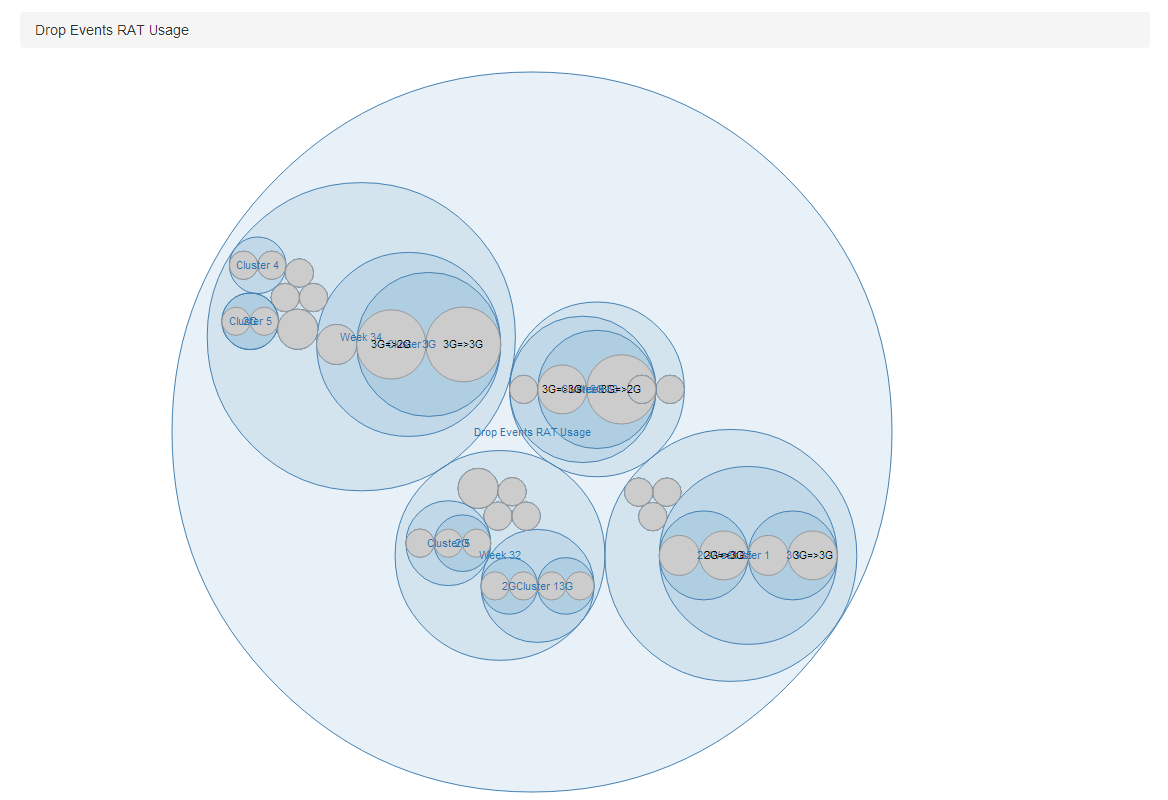
\includegraphics[scale=0.65]{chapter8/visualisation/circle_pack.png}
        \caption[Example Circle Pack output]
                {Example Circle Pack output, highlighting all the nodes. The 
               first node is the week, e.g. week 34.}
        \label{fig:circle_pack}
    \end{figure}
\end{landscape}


\newpage
\subsubsection{Dendrogram}

As with the Circle Pack diagram a dendrogram represents hierarchy through 
embedded nodes. A dendrogram is frequently used to illustrate the cluster 
arrangement formed by hierarchical clustering algorithms, although can be used 
in other ways.

Unlike the Circle Pack diagram, a dendrogram is not able to reveal the overall 
size of each element visually, and this has been shown via the raw value of 
events shown in brackets.

Figure \ref{fig:dendrogram} illustrates an example output.


% Landscape page
\begin{landscape}
  % Center image
  \centering 
    \begin{figure}[H]
      \centering
        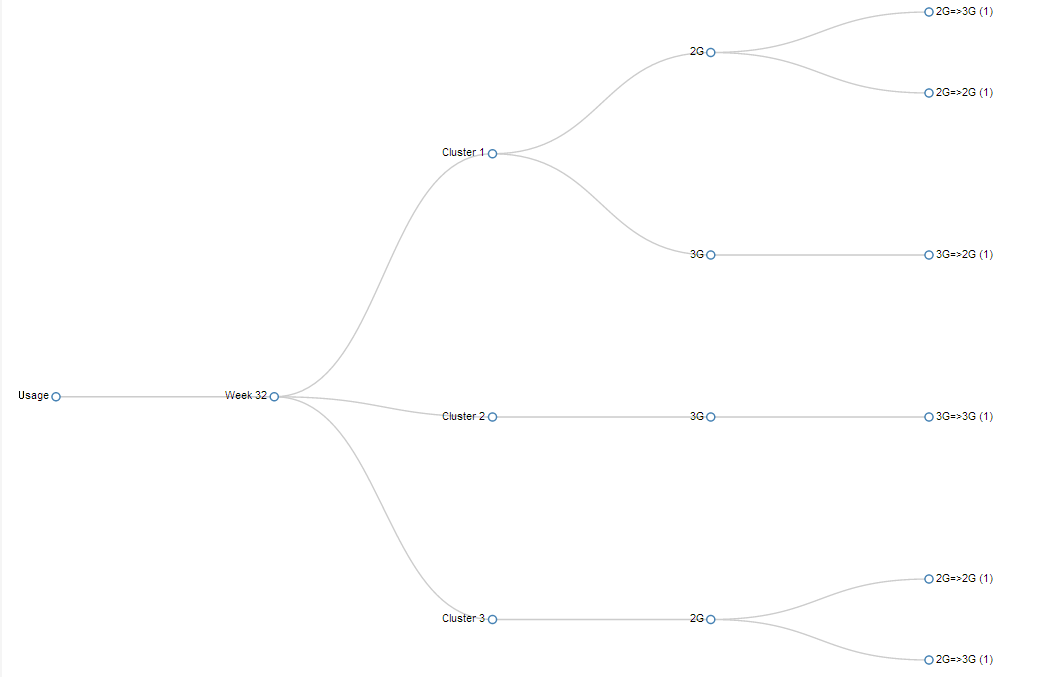
\includegraphics[scale=0.65]{chapter8/visualisation/dendrogram.png}
        \caption[Example Dendrogram output]
                {Example Dendrogram output, highlighting all the various for 
                the given week (week 32)}
        \label{fig:dendrogram}
    \end{figure}
\end{landscape}


\newpage
\subsubsection{Partition Chart}
A partition chart can thought of as an alternative to a pie chart. Although it 
looks more like a treemap, it more closely resembles the characteristics of a 
pie chart.

As with the previous charts, the partition chart supports hierarchical data. 
This allows the user to click upon a given area, and the chart will rearrange 
itself. This allows for a more bespoke, ``drilled down'' view to viewing the 
analysis.

Figure \ref{fig:partition_chart} highlights an example partition chart.

\begin{figure}[H]
  \centering
    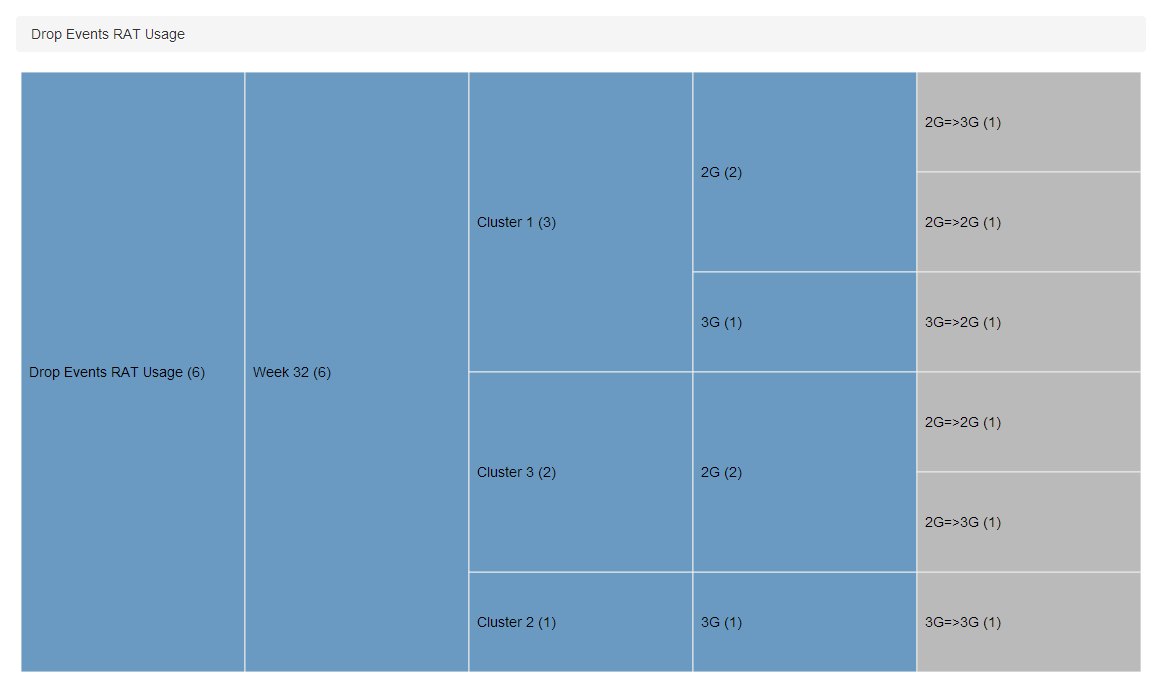
\includegraphics[scale=0.50]{chapter8/visualisation/partition.png}
    \caption[Example Partition output]
            {Example Partition output, highlighting all the nodes for the drop 
             events usage figures.}
    \label{fig:partition_chart}
\end{figure}


\newpage
\subsubsection{Treemap}
A treemap illustrates data as a set of nested rectangles. Like the partition 
chart, treemaps support hierarchical data structures.

Each square represents the total count of the events --- the larger the square 
the more events were found with the criteria. As with the partition chart, 
patterns within the data can be easily spotted. 

As a treemap grows, the efficiently of the use of space will also grow. The 
treemap implementation allows for a user to click upon a square, and it will 
rearrange itself, and as with many other charts will allow for a ``drilled 
down'' view.

Figure \ref{fig:treemap} highlights an example treemap.

\begin{figure}[H]
  \centering
    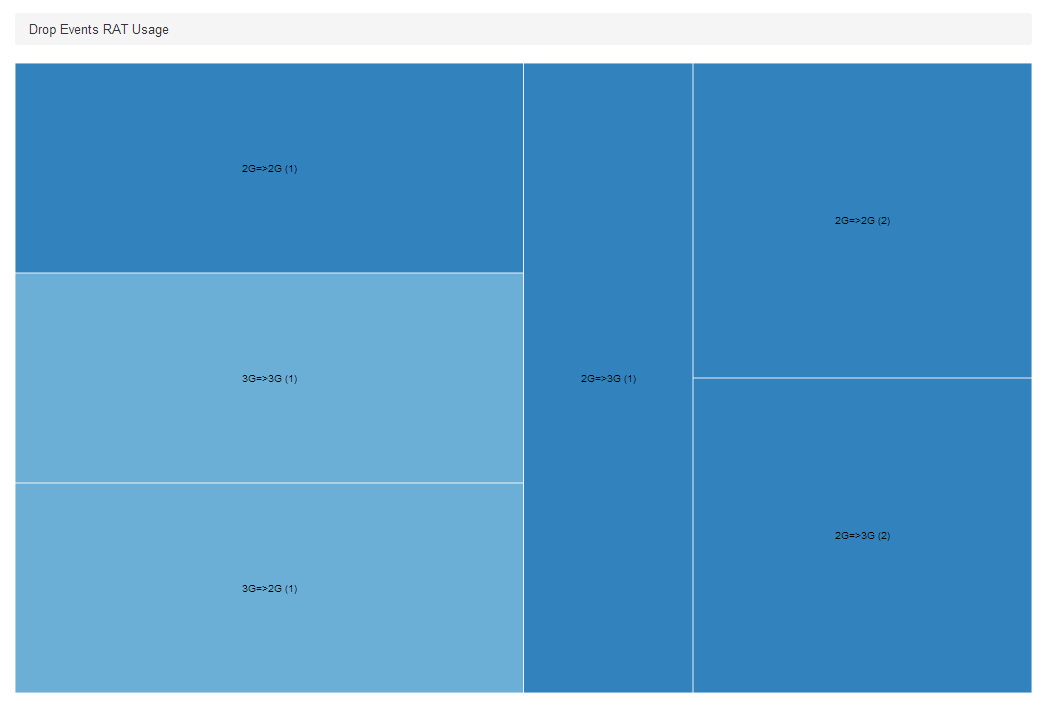
\includegraphics[scale=0.55]{chapter8/visualisation/treemap.png}
    \caption[Example Treemap output]
            {Example Treemap output, highlighting all the nodes for the drop 
             events usage figures.}
    \label{fig:treemap}
\end{figure}

% Chapter 4 - Requirements
\chapter{Requirements}
\label{chap:requirements}
There is a hierarchical approach that should be used in structuring 
requirements \citep{cadle10}. Table \ref{table:requirementsCategories} outlines
the main four categories:

\begin{table}[H]
  \begin{tabular}{|l|l|l|l|}
    \hline
    {\bf General} & {\bf Technical} & {\bf Functional} & {\bf Non-Functional} \\ 
    \hline
    Business constraints & Hardware & Data entry & Performance \\ 
    Business policies & Software & Data maintenance & Security \\ 
    Legal & Interoperability & Procedure & Legal and Access \\ 
    Branding & Internet & Retrieval & Backup and Recovery \\ 
    Cultural & ~ & ~ & Archiving and Retention \\ 
    Language & ~ & ~ & Maintainability \\ 
    ~ & ~ & ~ & Business Continuity \\ 
    ~ & ~ & ~ & Availability \\ 
    ~ & ~ & ~ & Usability \\ 
    ~ & ~ & ~ & Capacity \\
    \hline
  \end{tabular}
  \label{table:requirementsCategories}
\end{table}

Each of the four categories described in Table \ref{table:requirementsCategories}, 
will form the basis of this requirements chapter.


% General Requirements
\newpage
\section{General Requirements}
The general requirements are ones that define the business policies, standards 
and needs \citep{cadle10}. Many of the requirements are not related to this 
project, but will be noted for reference purposes.

\subsection{Business constraints}
The business constraints are the constraints that will directly effect this 
project. There are no constraints from BlackBerry, however there are time based 
constraints from the University.

\subsection{Business policies}
The business policies cover aspects such as business standards and business 
policy decisions. These are enforced to ensure consistency across is maintained 
across an organisation. This project has no requirements to deal with business 
policies.

\subsection{Legal}
\subsubsection*{Copyright, Designs and Patents}

In order to avoid various patent disputes, any third party resources, such as 
programming languages, development tools and external libraries will be only 
used if the licence associated with the item is of a non-proprietary agreement.

However there are some circumstances where by proprietary sources will have to 
be used for example the use of Visual Studio 2010. 

These sources will have been chosen to meet the interests of all parties 
involved, and where applicable the version of software will be taken into 
consideration. 

Any use of non-proprietary software must first be accepted by BlackBerry, to 
ensure that the correct licences are used.

All software released by this project will be under the New BSD Licence (also 
referred to as the BSD 3-Clause License). This license allows for 
re-distribution and use in both source and binary formats. 

The license also allows for the source code to be modified as long as the 
licence agreements are met.

\subsubsection*{Data Protection}
The Data Protection Act (1998) provides security for personal or business data 
that is stored electronically. In order for the project to continue, there will 
be various pieces of data required to fully test the system from BlackBerry. 
The data is to be transmitted via an encrypted form, and will not be passed on 
to any third parties. 

All data is of the property of BlackBerry unless otherwise stated.

\subsubsection*{Intellectual Property}
All intellectual property rights will belong to BlackBerry, once the project 
has been assessed by the university. This will allow for future modification 
and extension to the end deliverable from this project. Once the project is 
completed, the licence agreement can be updated to reflect BlackBerry’s 
business practice if required.

\subsection{Branding}
The branding requirement is concerned with the image and style promoted by 
BlackBerry. This would take into considerations such as style guides, fonts and 
logos. 

The end product is intended for internal use only (not for public use), and 
hence the branding requirements will not need to be followed.

\subsection{Cultural}
This section is devoted to BlackBerry's culture, such as management styles. As 
the project is not being developed within BlackBerry's facilities, the culture 
style is not required to be taken into consideration.

\subsection{Language}
This project will be completed utilising the English (British) language. 
Additional languages will not be supported.

% Technical Requirements
\newpage
\section{Technical Requirements}
Technical requirements state the technical policies and constraints to be 
adopted from BlackBerry \citep{cadle10}.

\subsection{Hardware}
The end product will not interact with any bespoke hardware, and therefore there 
are no hardware requirements.

\subsection{Software}
The end product should be able to run upon an existing internal server. The 
server in question, is a Microsoft Windows based operating system.

From talks with BlackBerry, it is apparent that there are a number of languages 
and tools that can be used to create the final product. However due to the 
Windows based environment that the end software product will be running on, it
was recommended that C\# would be used.

The advantage of using C\#, is the fact that C\# runs upon the Microsoft .NET 
framework. This means that as long as the production machine is running the 
same version of the .NET framework as the development machine, the tool should 
work with few issues. 

This is obviously a major advantage, as additional compilers, interpreters or 
parsers are simply not required. There would also be little setup overheads as
well.

\subsection{Interoperability}
The final software product is not expected to interact with BlackBerry's 
internal systems. The product will handle the importing of data from a given 
file. This is discussed in further detail in the Functional Requirements 
section. The product will not be required to communicate with other pieces of 
hardware.

\subsection{Internet}
The final software product will not require an internet connection in order to
work, and therefore BlackBerry's networking policies will not need to be taken
into consideration.

% Functional Requirements
\newpage
\section{Functional Requirements}
The functional requirements of a system are those that set out the features 
that any software solution should provide \citep{cadle10}. This is only 
intended to be a brief overview, a more detailed specification can be found 
within the specification section of this document.

\subsection{Data entry}
The gathering and recording of data will be handled by BlackBerry. The end 
product will not in any way need to gather data, however it will need to 
process a set of data found within a given file.

\subsection{Data maintenance}
As the gathering and recording of data is handled by BlackBerry, the requests 
for additional data or for the data to be changed, must be first authorised by 
BlackBerry. 

\subsection{Procedure}
New features, or analysis procedures that are outside of the project 
specification must be first authorised for use by BlackBerry.

\subsection{Retrieval}
The retrieval of data is concerned with the accuracy and integrity of the data.
In order to achieve high accuracy and integrity additional internal knowledge 
is required that is unable to be shared with third parties of BlackBerry. It is
therefore assumed that all data pushed from BlackBerry is correct.

% Non-Functional Requirements
\newpage
\section{Non-Functional Requirements}
The non-functional requirements deal with how well the solution will operate 
\citep{cadle10}. 

\subsection{Performance}
The performance of the system should be good, however it must be noted that the
system is intended to run as a service upon a server. The output data and 
analysis will be used by additional services which are not part of this 
project.

\subsection{Security}
All data handled by this project is strictly confidential, and must not be 
distributed in any form. This project will not handle database storage, as the
product is intended to interact with BlackBerry's secure network. 

All output data will be stored in files, that will be stored upon a secure 
revision control system, with access through a secure shell.

\subsection{Legal and Access}
Access permissions to data (such as being able to delete a particular piece of 
data from a live database), is not a requirement of this project.

\subsection{Backup and Recovery}
The project or it's data is not in anyway to be stored upon a portable data 
storage device, nor should it be stored upon publicly accessible cloud storage.

The project will make use of the git subversion system over a secure shell 
connection. This will ensure that:
\begin{enumerate}
  \item A copy of the project is stored upon a remote, secure server;
  \item Changes are able to be tracked;
  \item Issues and comments are able to be raised in a secure environment.
\end{enumerate}

The above measures will in effect be able to reduce against the loss, damage or 
theft of sensitive company information.

\subsection{Archiving and Retention}
The University will temporarily retain the project (software product and the 
final report) for assessment purposes only. Once the assessment of the project 
is completed the University will release the project and will no longer hold a 
copy of the project.

A copy of the project (excluding any input data) will be taken by the student 
for professional development purposes. 

\subsection{Maintainability}
All maintenance and related extensions to the project will be handled by 
BlackBerry as of Friday, 26th April 2013. This deadline has been set by the 
University as the final hand in date for the project.

\subsection{Capacity}
The end product should be able to handle data from multiple files, that could be 
representing multiple weeks worth of data. 

Each file can have any number of clusterable data, however files with limited
data may not produce results.

% User Requirements
\newpage
\section{User Requirements}
\label{sec:userrequirements}
All objectives have been set by BlackBerry, and have been combined into a 
requirements list. In order to sure that the most important development of the 
final product is undertaken first, a prioritisation system will need to be 
used.

MoSCoW was first developed by Dai Clegg \citep{clegg94}, and divides 
requirements into four categories \citep{brennan09} as outlined below:
\begin{itemize}
  \item Must
  \item Should
  \item Could
  \item Won't
\end{itemize}

The o's within the acronym are added to allow for easy pronounceability, and 
have no other purpose other than this. Each category is described in further 
detail below, along with each of the requirements outlined by BlackBerry.


\subsection{Must}
The Must category describes a requirement that {\bfseries must be satisfied} in
the final product, for the project to be considered a success 
\citep{brennan09}. 

The must requirements for this product are outlined below:
\begin{itemize}
  \item Design and develop an algorithm to cluster GPS coordinates.
  \item Compare RAT footprints of two data sets (products or pins) with each 
        set being N weeks’ worth of data and highlight differences in the RAT 
        usage/drop/fails along the route.
  \item Compare MIX\_BAND (Frequency bands) footprints of two data sets and 
        highlight differences in usage/drops/fails between sets.
\end{itemize}


\subsection{Should}
The Should category describes a requirement 
that is classed as a {\bfseries high-priority item} that should be included in 
the final product if at all possible \citep{brennan09}. These requirements are
often critical, but can be satisfied in other ways if needed. 

The should requirements for this project are outlined below:
\begin{itemize}
  \item Compare two sets of call data and create drop/failure clusters, 
        highlighting the differences. 
  \item Ability to tag drops/fails with classification attributes and even 
        compare based on attributes.
\end{itemize}


\subsection{Could}
\label{sec:could}
The Could category describes a requirement that is considered {\bfseries 
desirable but not necessary} \citep{brennan09}. This will be included if 
resources permit (both time and technical/non-technical). 

The could requirements for this project are outlined below:
\begin{itemize}
  \item Velocity differences along route.
  \item Utilise a number of charting techniques to display the analysis 
        results.
  \item Plot a map for all call attempts and call ends (success/fail) for a 
        given period of time, for different devices.
  \item Allow the user to filter the clustering down (e.g. show only call 
        drops).
\end{itemize}


\subsection{Won't}
The Won't category describes a requirement that will not be implemented in a 
given release. This is usually in the form of an agreement between all the 
project stakeholders \citep{brennan09}. However the requirements may be 
implemented in the future. 

The won't requirements for this project are outlined below:
\begin{itemize}
  \item Integration with current internal BlackBerry testing systems.
\end{itemize}


% Assumptions 
\newpage
\section{Assumptions}
The following assumptions will be made throughout this project:
\begin{itemize}
  \item The programmer has a limited knowledge of the mobile network;
  \item The input data generated by the client is correct.
\end{itemize}



% Chapter 5 - Product Specification
\chapter{Product Specification}

Within this chapter the a formal product specification will be formed, based 
upon BlackBerry's requirements (chapter \ref{chap:requirements}). The 
specification will identify the functionality of the software product, as well
as any data requirements.

% Product Specification
\newpage
\section{Product Specification}

Within section \ref{sec:userrequirements} the user requirements as defined by 
BlackBerry were prioritised using the MoSCoW prioritisation system. In order to 
ensure that the final product is delivered to the expectation of the client, a
product specification will be proposed. 

The product specification below follows a similar layout to what was seen in 
section \ref{sec:userrequirements} (User Requirements). Prioritising the 
various objectives within the system, can help to ensure that the most 
important aspects of the system are developed first. It also highlights any 
potential issues that may occur.


\subsection{Must}
\begin{itemize}
  \item Parse any number of KML files (one or more) at any one time;
  \item Convert each Placemark found within each KML file to an Event;
  \item Cluster all the Events upon a weekly basis;
  \item Cluster all the Events upon a product basis;
  \item Highlight the overall differences of RAT usage between weeks and 
        products;
  \item Highlight the overall differences of Mix Band usage between weeks and 
        products;
  \item Highlight the overall differences of Start RRC State usage between 
        weeks and products;
  \item Highlight the inter-cluster differences of RAT usage between weeks and 
        products;
  \item Highlight the inter-cluster differences of Mix Band usage between weeks 
        and products;
  \item Highlight the inter-cluster differences of Start RRC State usage  
        between weeks and products.
\end{itemize}


\subsection{Should}
\begin{itemize}
  \item Visualise the differences of data to allow for easy comparison when 
        trying to compare upon a weekly basis;
  \item Visualise the differences of data to allow for easy comparison when 
        trying to compare upon a product basis;
  \item Produce an output KML file highlighting all clusters and events. Each
        cluster must visually show it's radius;
  \item Produce a heatmap to highlight the strong areas of event density.
\end{itemize}


\subsection{Could}
\begin{itemize}
  \item Allow the use to easily apply filters to the analysed data to help 
        further ``drill down'' into the analysis;
  \item Highlight the change in velocity differences along the test route.
\end{itemize}


\subsection{Won't}
\begin{itemize}
  \item Directly interact with any internal BlackBerry data sources.
\end{itemize}

% Data Definition
\newpage
\section{Data Definition}

Within section~\ref{sec:userrequirements} (page~\pageref{sec:userrequirements}), 
the various system requirements were highlighted. However the data requirements 
were not discussed. 

In order to cluster the data, the tool will need to access the associated call 
logs. Due to legal reasons and a lengthy authorisation processes, connecting 
directly to a BlackBerry data source was deemed to be out of the scope of this
project. 

However in order to ensure the tool is correctly working, BlackBerry have 
agreed to supply some real, anonymous data for testing purposes. The data will 
be supplied within a set KML format.

The KML file format is ``used to display geographic data in an Earth browser 
such as Google Earth, Google Maps'' \citep{google:KML}. The KML structure is 
tag-based which contains various elements and attributes that can be nested, 
and is an XML extension.

{\bf All} tags are case-sensitive and {\bf must} appear exactly as they are 
listed in the KML API reference. Within a given element, tags must also appear 
in the same order that is shown in the API reference. 

An example snippet showing an Event is shown below.

% Define XML Colour Scheme
\definecolor{gray}{rgb}{0.4,0.4,0.4}
\definecolor{pink}{HTML}{008080}
\definecolor{darkblue}{rgb}{0.0,0.0,0.6}
\lstdefinelanguage{XML}
{
  basicstyle=\ttfamily\small,
  columns=fullflexible,
  showstringspaces=false,
  commentstyle=\color{gray}\upshape
  morestring=[s]{>}{<},
  morecomment=[s]{<?}{?>},
  stringstyle=\color{black},
  identifierstyle=\color{pink},
  keywordstyle=\color{darkblue},
  morekeywords={Placemark,Point,coordinates,ExtendedData,SimpleData,
                Document,name,kml}
}

% Import the KML Template
\begin{lstlisting}[language=XML]
<Placemark>
  <Point>
    <coordinates>-0.2341408,51.3653237,0</coordinates>
  </Point>
  <ExtendedData>
    <SimpleData name="device">9800</SimpleData>
    <SimpleData name="pin">03dcde00</SimpleData>
    <SimpleData name="timestamp">07/08/2012 00:00:00<SimpleData>
    <SimpleData name="reference">true</SimpleData>          
    <SimpleData name="type">drop</SimpleData>
    <SimpleData name="start_rat">WCDMA</SimpleData>
    <SimpleData name="end_rat">WCDMA</SimpleData>
    <SimpleData name="start_mix_band">10812</SimpleData>
    <SimpleData name="end_mix_band">10787</SimpleData>
    <SimpleData name="start_rrc_state">IDLE<SimpleData>
  </ExtendedData>
</Placemark>
\end{lstlisting}


Each Placemark represents an event, with each Placemark containing data about 
the location of the event, and additional ``meta-data''. The location of the 
data is stored within the Point tag, and the additional ``meta-data'' is stored 
within the ExtendedData tag. 

The coordinates are expressed as decimals, and follow the following template:

\begin{lstlisting}[language=XML]
  <coordinates>longitude,Latitude,Altitude</coordinates>
\end{lstlisting}

{\em Note: Data that sits in between the coordinates tag cannot have {\bf any} 
additional whitespace.}

The additional ``meta-data'' is stored as a list of SimpleData items. The 
order of the elements is imperative, and {\bf must} be maintained. Each of the 
SimpleData tags must be present, even if no data is stored. If no data is 
stored, then an empty tag must be present.

Each of the SimpleData tags are discussed in more detail below:
\begin{itemize}
  \item {\bf device} \\
        The Name of the device.
  \item {\bf pin} \\
        The Personal Identification Number (PIN) of the device.
  \item {\bf timestamp} \\
        The time stamp of the event in the format `DD/MM/YYYY HH:ii:ss'
  \item {\bf reference} \\
        Whether or not the device is a reference device
  \item {\bf type} \\
        The type of call, one of `Call Drop', `Setup Failure', `Successful Call'
  \item {\bf start\_rat} \\
        The Start RAT of the event
  \item {\bf end\_rat} \\
        The End RAT of the event
  \item {\bf start\_mix\_band} \\
        The Start MixBand of the event
  \item {\bf start\_rrc\_state} \\
        The Start RRC State
\end{itemize}

~\\
A single KML file can contain any number of Placemark values, and must be 
wrapped inside the KML and Document tags, as show below. 

\begin{lstlisting}[language=XML]
<kml xmlns="http://www.opengis.net/kml/2.2">
  <Document>
    <name>KML Filename</name>
    <Placemark>
      ...
    </Placemark>
    <Placemark>
      ...
    </Placemark>
    <Placemark>
      ...
    </Placemark>
    <Placemark>
      ...
    </Placemark>
  </Document>
</kml>
\end{lstlisting}

% Chapter 6 - Development Method
\chapter{Development Methodologies}

In order to achieve all the goals that this project has set out to achieve, a 
software development process will be required to be implemented and followed. 
The advantages of structuring such a software development project into a set of 
defined processes far outweighs the disadvantages \citep{knott_dawson99}. 

These defined processes form part of a process model, to which a process model 
can be described as:
\begin{itemize}
	\item a conquer and divide approach of problems into tasks at each stage;
	\item adding an element of control and planning;
	\item allowing for progress to be mapped visually;
	\item providing a structured approach to development;
	\item allowing for a higher quality of code and documentation to be produced.
\end{itemize}

According to \citet{elliott04}, the oldest formalised methodology for building 
software products was known as the systems development life cycle (SDLC). The 
SDLC methodology utilises a structured and methodical approach, where by each 
stage of the life cycle is to be carried out rigidly and in order.

Within this chapter, various software development methodologies will be discussed 
and evaluated, ultimately leading to a software development methodology being 
chosen to use within this project.

% Waterfall Methodology
\newpage
\section{Waterfall}
A fundamental aspect to the waterfall model is the fact that the project is 
expected to progress down the primary path \citep{sergei:2012:Online}. The 
primary path is the most commonly used path through out a system. By 
highlighting the primary path, the major processes and tasks are easily mapped
out, a clear indication of what exactly is required to be completed.

The waterfall model contains six main phases --- requirements analysis, 
specification, design, coding, testing and implementation \citep{dawson09}. 
Deliverables are achieved as the flow down the primary path is completed. 

It is possible however for a reverse flow. This reverse flow represents a 
change applied to a prior deliverable, which was only recognised in the 
deliverable after the change is required in. This is known as rework, and can 
result in both the current deliverable and previous deliverables to be 
repeated.

\begin{figure}[H]
  \centering
  \vspace{-40pt}
  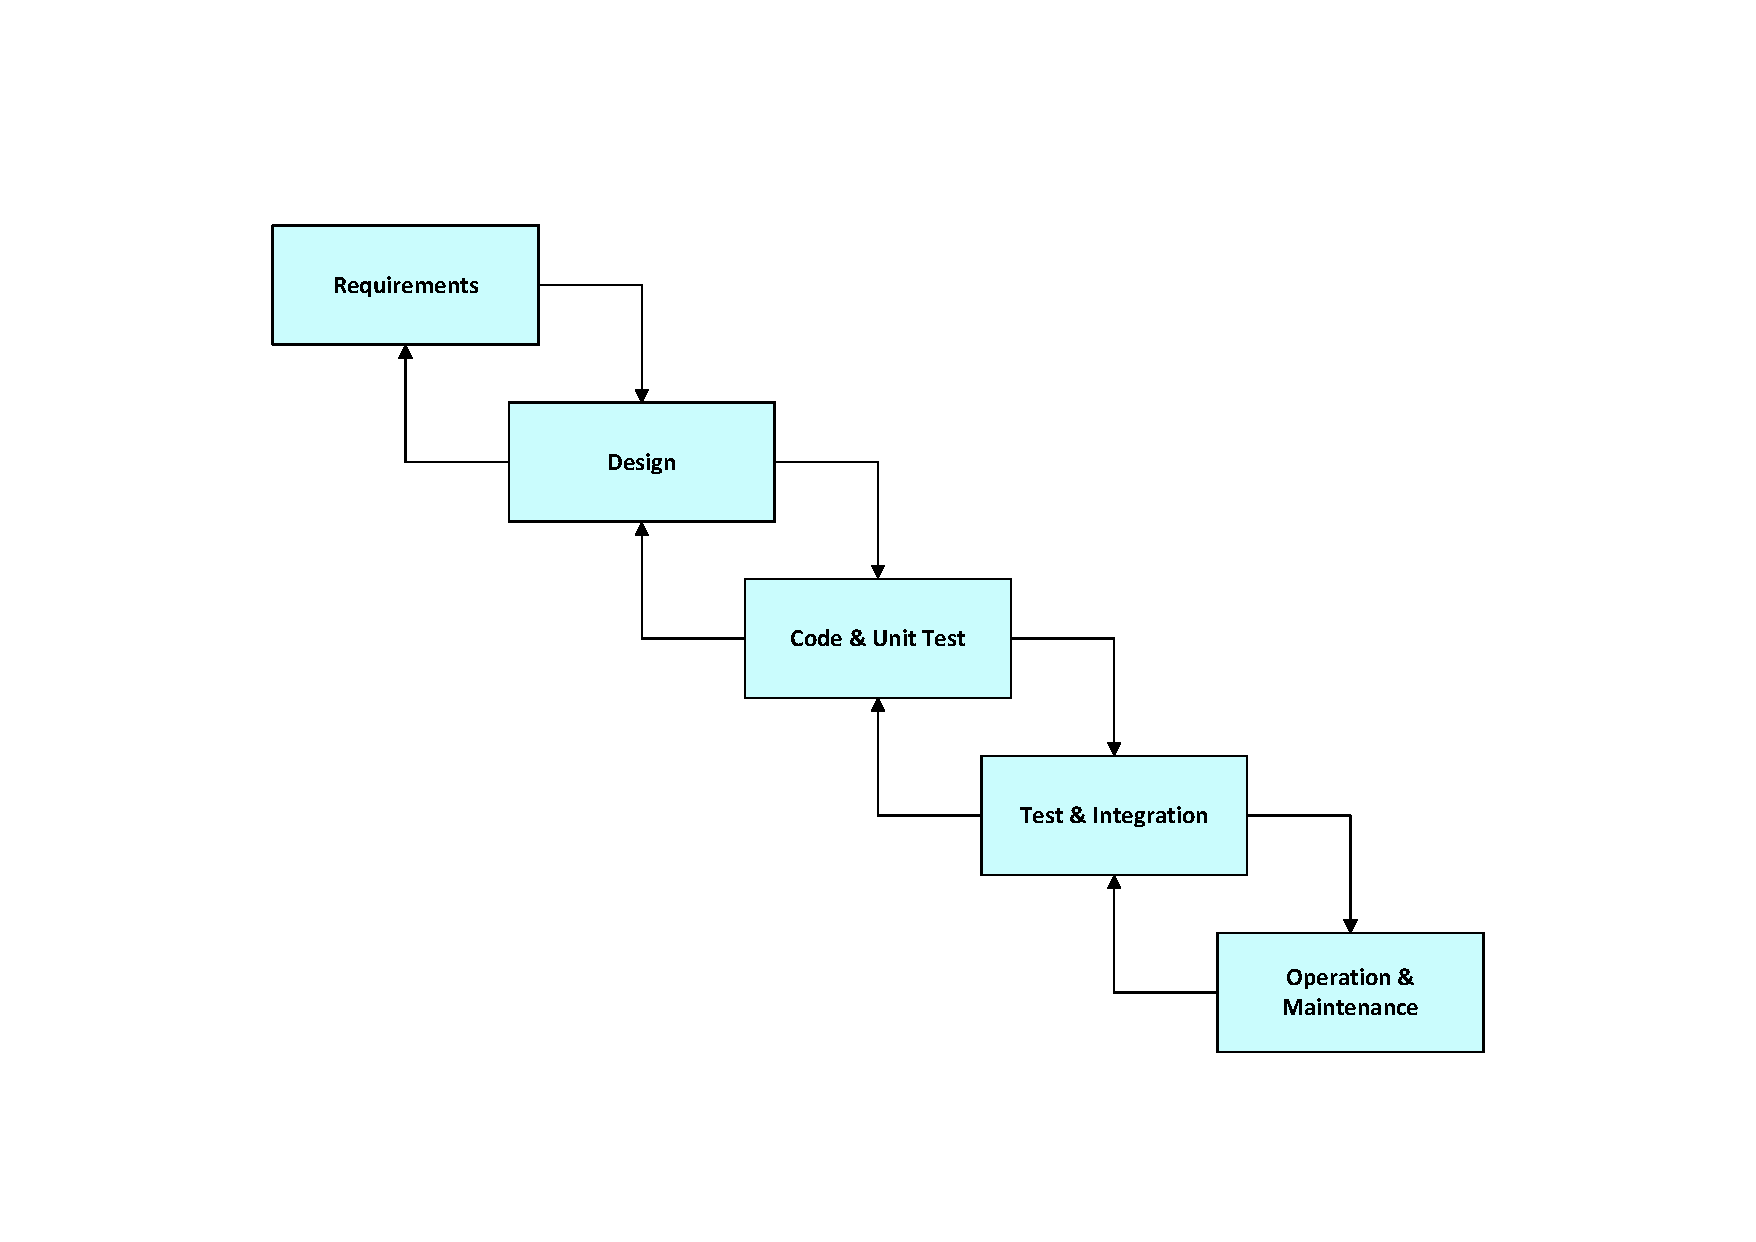
\includegraphics[width=\linewidth]{chapter6/waterfall.pdf}
  \vspace{-40pt}
    \caption[Waterfall methodology]
      {Waterfall methodology highlighting the ``flow'' through the various 
      sections that make up a software development project.}
\end{figure}

\subsection{Advantages}
The waterfall model is the most commonly used methodology due to the following 
reasons \citep{alam:2012:Online}:
\begin{itemize}
	\item Documentation is produced at every stage, allowing for anyone to join
        the project at any time to have full understanding;
  \item Minimum resources are required to implement this model, and is simple
        to implement and follow;
  \item Testing is completed after every major stage of software development.
\end{itemize}

\subsection{Disadvantages}
However, the disadvantages of this methodology are \citep{alam:2012:Online}:
\begin{itemize}
	\item The model works well if there is no reverse flow. Reverse flow can 
        cause time delays;
  \item The model assumes that the client know exactly what they want, in 
        reality this is not the case;
  \item A working model of the software is not complete, until the end product 
        has been finished.
\end{itemize}

% Incremental Methodology
\newpage
\section{Incremental}
The incremental software development methodology is an evolutionary extension 
of the waterfall model \citep{pressman09}. 

The main idea behind this development methodology is that developments are made
in increments, with each increment proving some additional functionality. This
additional functionality often only contains a small progression towards the 
final goal (or product).

Using an incremental approach allows the client to provide feedback, and thus 
the feedback be integrated into the product during development 
\citep{elliott04}. This incremental process continues until the final, 
completed product has been delivered. 

\begin{figure}[H]
  \centering
  %\vspace{-80pt}
  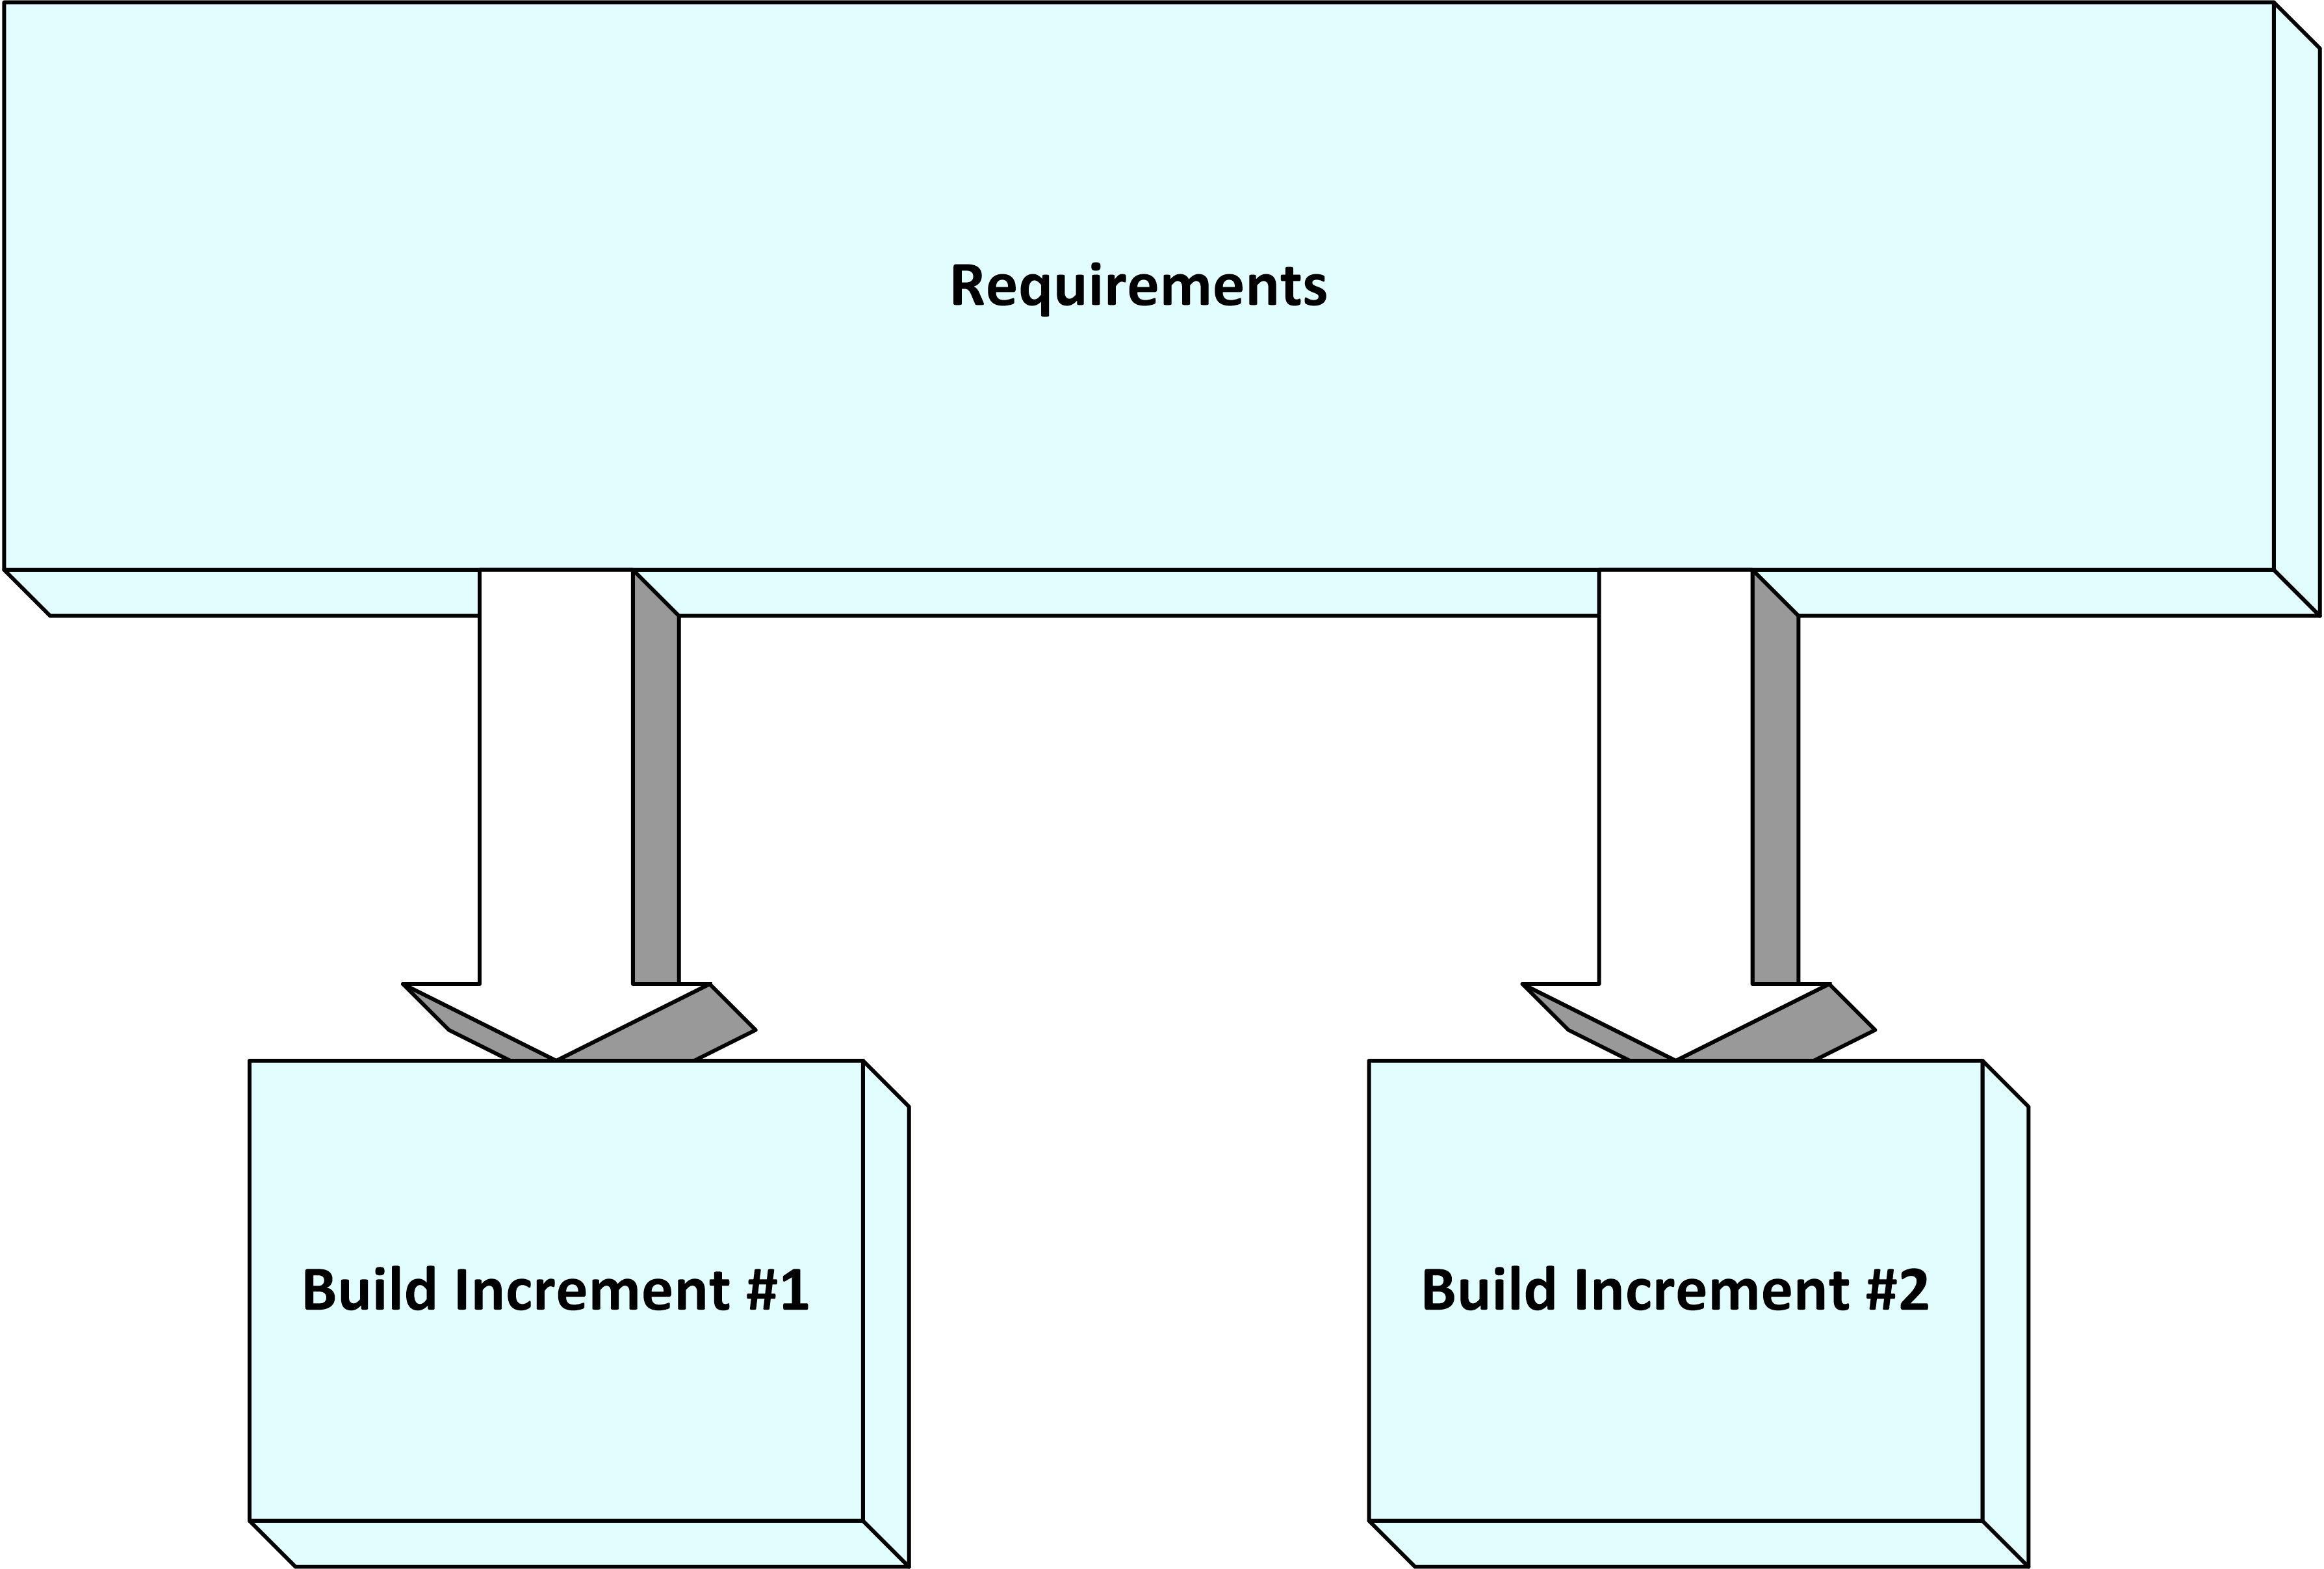
\includegraphics[scale=0.6]{chapter6/incremental.png}
  %\vspace{-60pt}
    \caption[Incremental methodology]
      {The incremental methodology allows for the requirements to be segmented 
      into an incremental series of the ``products''.}
\end{figure}

\subsection{Advantages}
The incremental software development methodology could be regarded as having 
the following advantages \citep{elliott04,SDT:2012:Online}:
\begin{itemize}
	\item The user is able to get an early idea of the system's capabilities;
	\item Early and continuous feedback is available from the client;
	\item It allows for more accurate planning, and slippage is easier to spot 
        due to the more frequent deadlines;
	\item It can be easier to test and debug, as any changes that are made within 
        an iteration are small;
	\item The user is able to learn how to use the system ``on the go'' rather 
        than in ``one go''.
\end{itemize}

\subsection{Disadvantages}
There are a number of disadvantages when utilising the incremental software 
development methodology \citep{elliott04,sergei:2012:Online}:
\begin{itemize}
	\item Development can occur for long periods of time, which might exceed the 
        original budget;
	\item Problems related to the system architecture could arise, if additional 
        functionality is added which was not 
				evident in earlier prototypes;
	\item The client may point out too many improvements, which would cause the 
        project to overrun or be completed not meeting the original 
        specification.
\end{itemize}

% Prototyping Methodology
\newpage
\section{Prototyping}
Prototyping is used when there is uncertainty about the technical solution to 
a problem \citep{dawson09}. 

It can be often useful to perform a number of experimental prototypes in order 
to gain understanding and knowledge, such as working on a new hardware platform
or developing a new algorithm. 

The prototyping software development methodology allows for many ideas and 
theories to be implemented, tested and evaluated. There are two main forms of 
prototyping, throw-away prototyping and evolutionary prototyping.

\subsection{Throw-away prototyping}
Once a prototype has been developed, the product associated with the prototype 
could be thrown away, with the actual development of the desired product 
starting from a blank ``canvas''.

\subsubsection{Advantages}
\citet{knott_dawson99} mention the following list of advantages over other 
software development methodologies: 
\begin{itemize}
  \item Errors and omissions in the requirements specification can be quickly 
        fixed;
  \item An artificial is produced quickly (keeping the client happy);
  \item The prototype is able to test the feasibility of the product;
  \item Alternatives of a various prototypes can be compared;
  \item Allows for improvement of communication between the developer and the 
        client.
\end{itemize}

\subsubsection{Disadvantages}
\citet{dawson09} highlights that there are a number of issues with the 
throw-away prototyping methodology, as highlighted below:
\begin{itemize}
  \item The prototype may contain a number of bugs;
  \item The prototype might look good, but technically could be poor. If it was 
        integrated into the system, then this could lead to poorly structured 
        code.
  \item Prototype development within a different language or system to the 
        final implementation may allow for technical differences to occur.
\end{itemize}

\subsection{Evolutionary prototyping}
Unlike the throw-away prototyping, a prototype could be developed further into
the final desired product. Utilising this idea, is known as evolutionary 
prototyping.

\subsubsection{Advantages}
The advantages are generally the same as the advantages found within the 
throw-away prototyping methodology with the following addition:
\begin{itemize}
  \item Any code that is developed, is reused and improved.
\end{itemize}

\subsubsection{Disadvantages}
As with the advantages, the disadvantages are generally the same as the 
advantages found within the throw-away prototyping methodology with the 
following addition:
\begin{itemize}
  \item A well structured design of code is required so that it can be 
        developed and allow for the evolution process to occur.
\end{itemize}

% Agile Methodology
\newpage
\section{Agile}

The agile software development methodology is designed to "reduce risk by 
delivering software systems in short bursts or releases" \citep{dawson09}. 

The concept behind the agile software development is to reduce the total weight
time that clients have to endure, by releasing working systems in as little 
time as possible. 

Each iteration may not contain a full working system, but it will contain a 
partial system, that could be used by the client. Agile methods are suited to 
projects that have unclear or rapidly changing requirements \citep{dawson09}.

\subsection{Advantages}
\citet{dawson09} states that the main principles of the agile software 
development methodology is as follows:

\begin{itemize}
	\item The methodology surrounds the concept of regular face-to-face meetings
        (as opposed to in-depth documentation);
	\item A close working relationship between the client and the developers;
	\item A short iterative time scale (usually weeks rather than months or 
        years);
	\item Easily able to change the requirements at any stage.
\end{itemize}

\subsection{Disadvantages}
However, \citet{dawson09} also states that the agile software development 
methodology does have it's problems:
\begin{itemize}
	\item There can be a limited amount of documentation, as this step is usually 
        skipped to save time;
  \item The uncertainty of a specification may lead to poor code and/or 
        structure.
\end{itemize}

% Extreme Programming Methodology
\newpage
\section{Extreme Programming}
Extreme Programming is a software development methodology intended to improve 
upon the agile methodology. It attempts to do this by maintaining high software 
quality whilst also maintaining high responsiveness to changing client 
requirements \citep{knott_dawson99}.

As found in agile development, there are many frequent release, and development 
is completed in short cycles, intended to improve productivity and to introduce 
check points (client requirements can be changed).

\subsection{Advantages}
The extreme programming software development methodology shares the same 
advantages as the agile and the evolutionary prototyping methodologies.

\subsection{Disadvantages}
As with the advantages, the disadvantages of the extreme programming methodology 
are shared amongst the agile and the evolutionary prototyping methodologies.

% Summary
\newpage
\section{Summary}
In order to achieve the best product possible, it is clearly evident that the 
client must be kept in the loophole as often as possible. This allows for any 
revisions, modifications, and changes to be considered and implemented with as 
little delay as possible.

Although this project has some well defined requirements, the details of the 
requirements are incomplete in some areas. However some key details have 
already been set, such as the programming language to be used and the target 
system. 

The rule of thumb states that if uncertainty is high then the use of an 
evolutionary approach is recommended \citep{hughes_cotterell09}. As well as 
this, the incremental approach seems to be an ideal methodology to utilise. 
The incremental methodology is ideal for projects that have a tight schedule 
\citet{hughes_cotterell09}.

Although the schedule of the project is not necessarily tight, it does contain 
a lot of potentially time consuming design research. By utilising the 
incremental methodology as a fundamental methodology, this should allow for 
small incremental developments to occur, with little work to re-complete if the
original path is later deemed to be incorrect.

Within each increment, an evolutionary prototype approach will be taken. The 
main reason for this is that it allows for development and research to coexist 
side by side. If the research pays off, then it's output can directly be 
utilised within the final published product.

% Chapter 7 - Design
\chapter{Design}

This section will focus upon the design of the various artifacts in order to 
successfully complete this project. The artifacts will be expressed utilising 
the Unified Modeling Language (UML).

% Primary Path
\newpage
\section{Primary Path Analysis}

In order to correctly and fully design a system as large as the one proposed, 
a sound understanding of the main process is required. The main process will 
be regarded as the scenario, which is ``a sequence of events or actions'' 
\citep{lunn03}. The scenario will contain various smaller scenarios which will 
be analysed separately. The main scenario is outlined below:

\begin{enumerate}
  \item Input data
  \item Cluster data
  \item Analyse the clustered data
  \item Output analysis
\end{enumerate}

Typically scenarios could be performed in any order, however the main scenario
outlined above can only be performed in one order. For example, in order for 
the analysis of the clustered data to happen, the data must first be clustered.

Another example is that data can only be clustered if data was given to the 
scenario in the first place, i.e. clustering of non-existent data could not 
happen. 

Now that the main scenario has been defined, the primary path of the entire 
system can now be formed. The primary path is a path through a system that is 
most commonly used, with a few variances \citep{lunn03}. 

The primary path for the Clustering Analysis Tool is outlined below:

\begin{enumerate}
  \item Import data set
  \item Cluster the data set
  \item Analyse clustered data set
  \item Create analysis charts
\end{enumerate}

The primary path outlined above is very generic with regards clustering of the 
the data set. The reason for this is that the clustering upon the data set can 
be applied in more than one way. 

Firstly the data can be clustered upon a week by week basis. This means that 
when analysed, the time stamp of the event is taken into consideration. This 
could result in a cluster that was found during multiple spanning weeks.

Finally, the data can be clustered upon a product basis. This means that when 
analysed, the device name (product name) is taken into consideration. This 
could result in multiple week's worth of testing being grouped by the device 
name rather than by the time stamp. 

Both of these ``in-depth'' paths can be thought of as alternative paths. The 
alternative path will contain subtle changes to the primary path 
\citep{lunn03}. The alternative paths for both a week by week analysis and a 
device based analysis can be seen shown below.

\subsection*{Week-by-Week Analysis}
\begin{enumerate}
  \item[2.1.1] Cluster the data set as an entire entity
  \item[2.1.2] Group the clustered data by the week numbers
\end{enumerate}

\subsection*{Product-based Analysis}
\begin{enumerate}
  \item[2.1.1] Cluster the data set as an entire entity
  \item[2.1.2] Group the clustered data by the device name
\end{enumerate}
~\\
The primary and alternative paths outlined above are a relatively simple, and 
yet powerful way of applying the general ideas behind the system. Both of 
these paths will be actively referred to in both the activity diagrams and use 
case diagrams found in the following sections.

% Activity Diagrams
\newpage
\section{Activity Diagrams}

Primary path analysis ensures that the exceptional and common paths throughout 
a system are identified \citep{lunn03}. Activity diagrams take these paths and
break them up into easy to follow, manageable processes.

An activity is a task in a process that allows for small meaningful work to 
happen. A process may have a number of activities linked together to form a 
work flow \citep{lunn03}.

\subsection{Import KML}
Figure \ref{fig:importkmlactivity} illustrates the simple action of importing 
the KML file into the system. In order to obtain the values from the file, a 
KML parser (or more precisely an XML Parser) is required. 

The parser will attempt to read each `Placemark' found within the file, and 
will try to read any additional meta data supplied.

Each placemark tag will be required to be converted to an Event object, so that 
the Events can be clustered.

\begin{figure}[H]
  \centering
    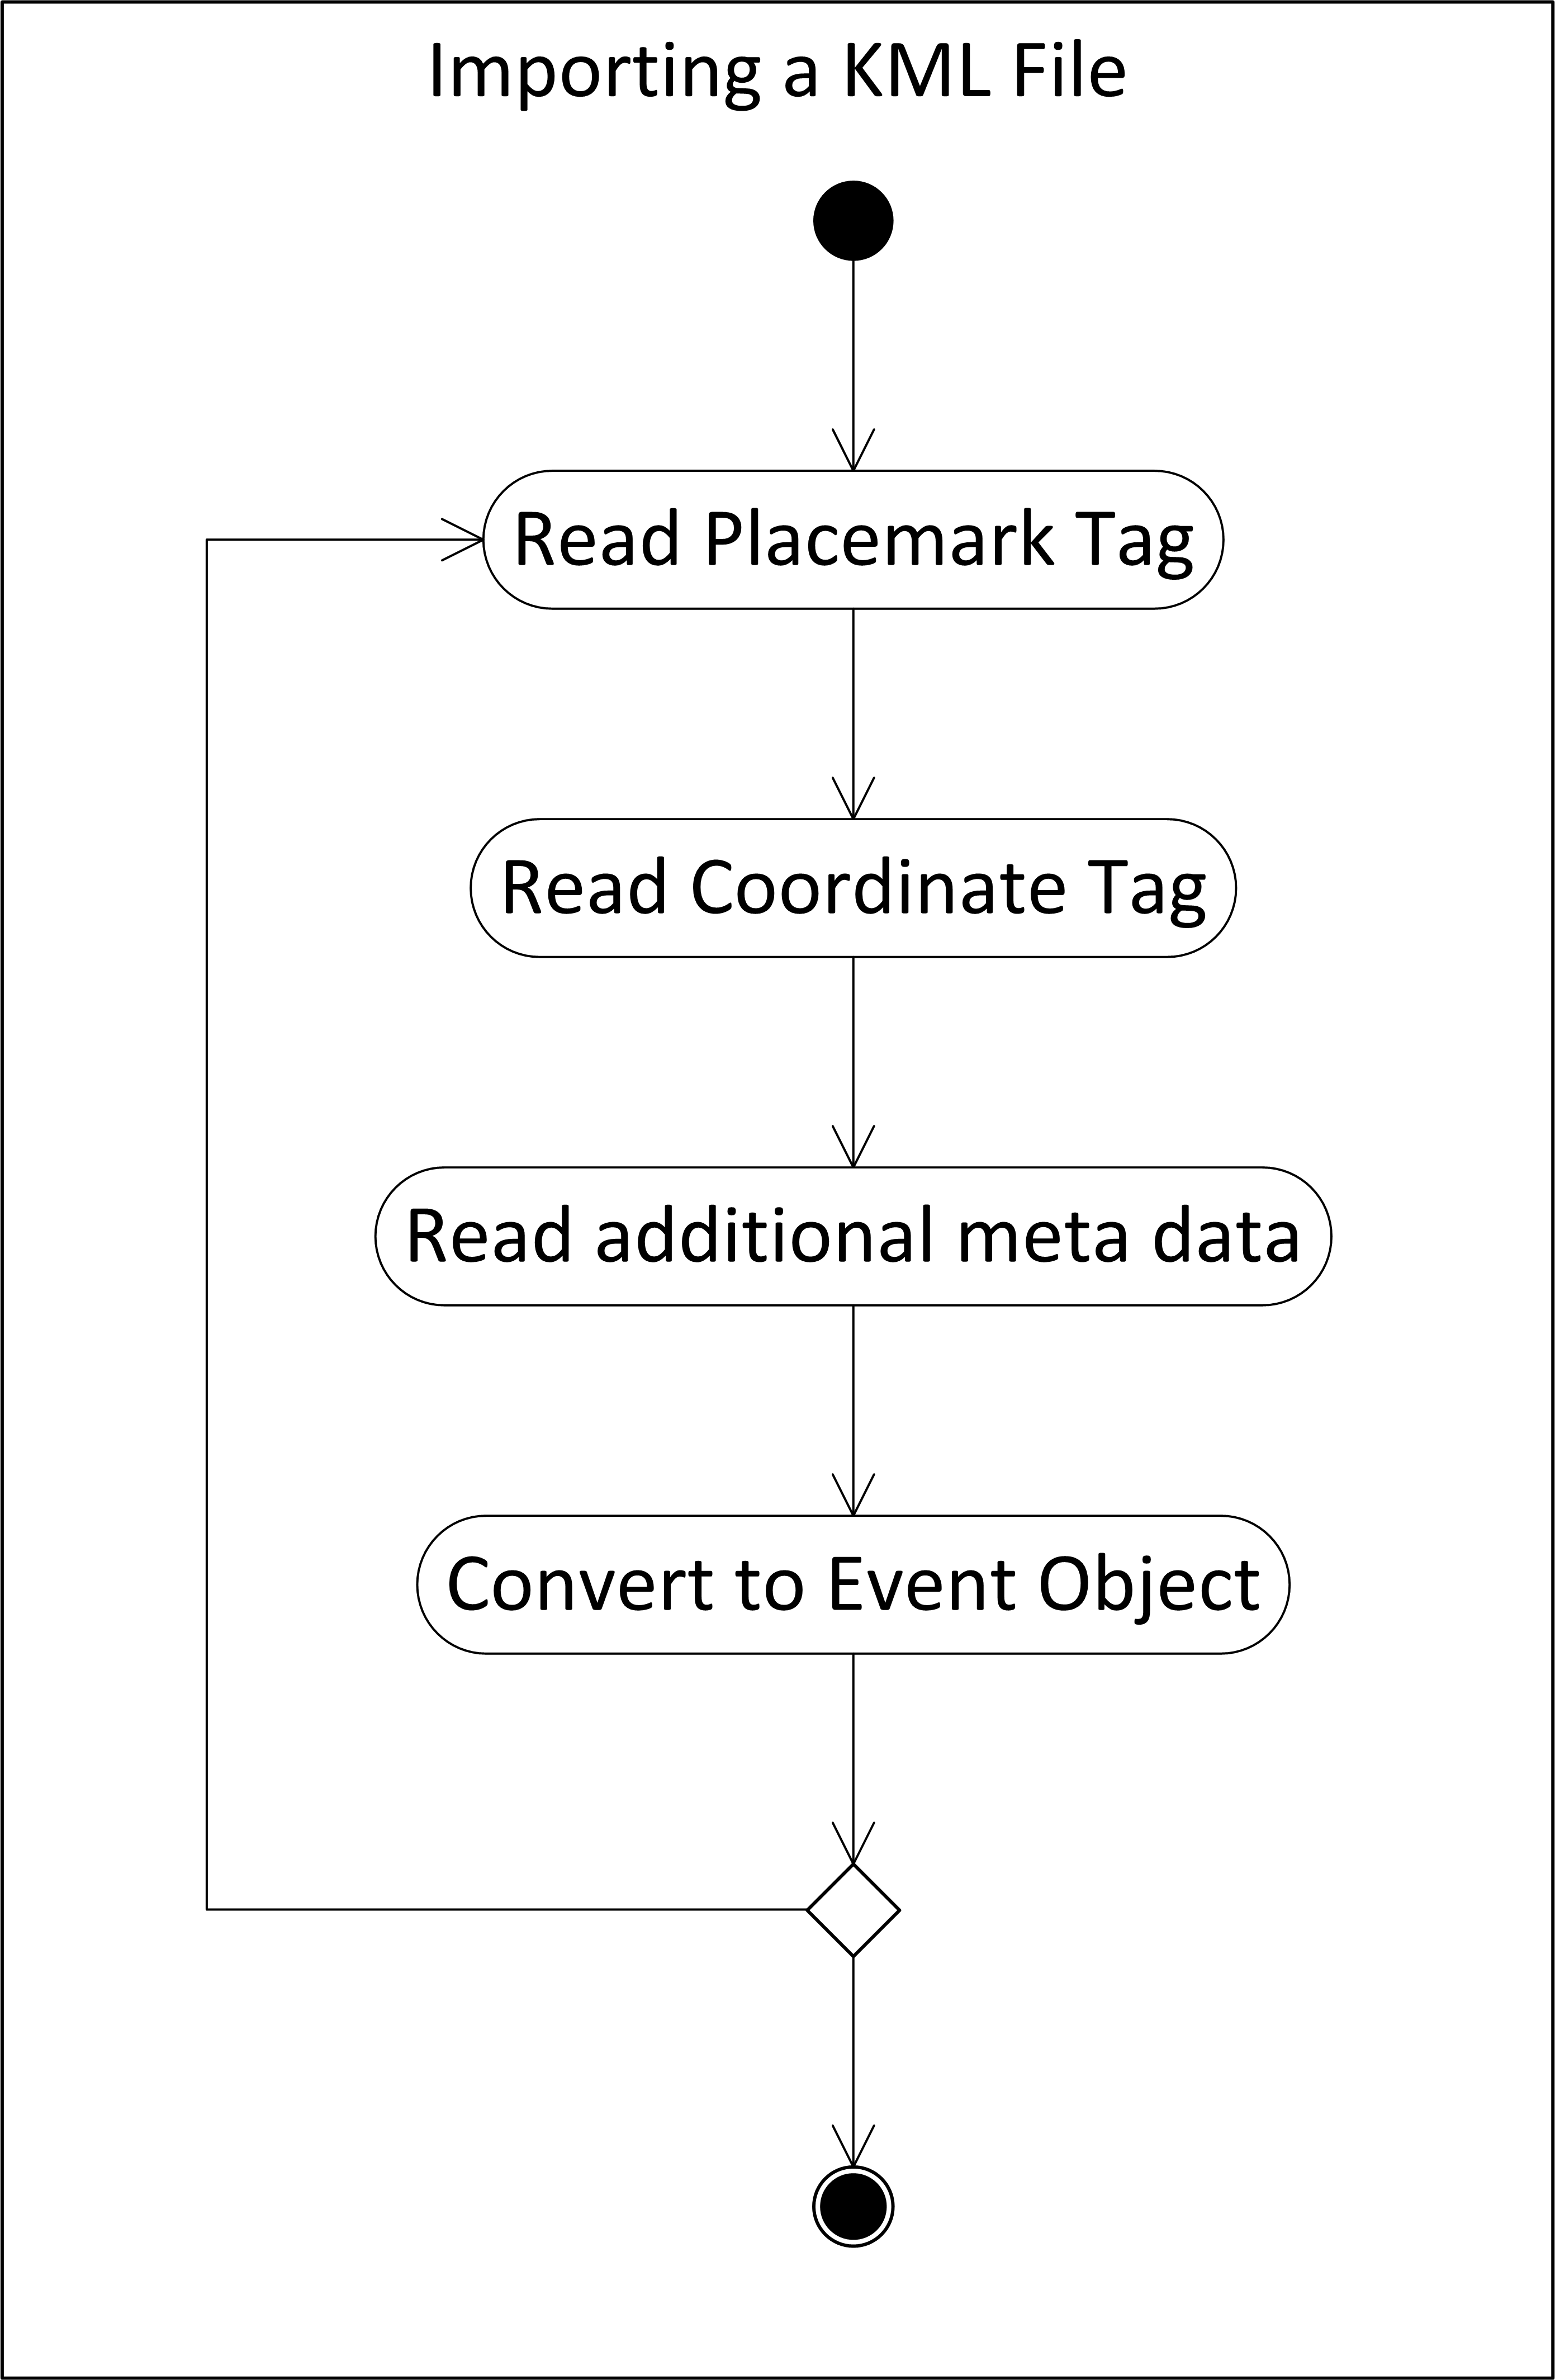
\includegraphics[scale=0.9]{chapter7/activity/import_kml.png}
    \caption[Importing a KML File activity diagram]
            {An activity digram highlighting the various actions that are 
             required to be taken in order to import a KML file}
    \label{fig:importkmlactivity}
\end{figure}


\subsection{Cluster Data}
Figure \ref{fig:clusterdataactivity} highlights the activity for clustering a 
set of Events using the DBSCAN algorithm. 

The algorithm will visit all points within the dataset, and for each 
unvisited point a neighbourhood visit will occur.

This means that the intra-cluster similarity will be calculated, and if it is 
deemed that two objects are related they will be placed into the same cluster.

All points that are deemed to be noise, will be separated from the resulting 
clusters. A noise point is one that does not fit into the neighbourhood of 
another point.

Border points are assigned upon the fly (rather than at the end of the 
clustering process) based upon the cluster that they are the closest to. The 
distance is based upon the centroid of the cluster (average of all objects 
within a cluster).

\begin{figure}[H]
  \centering
    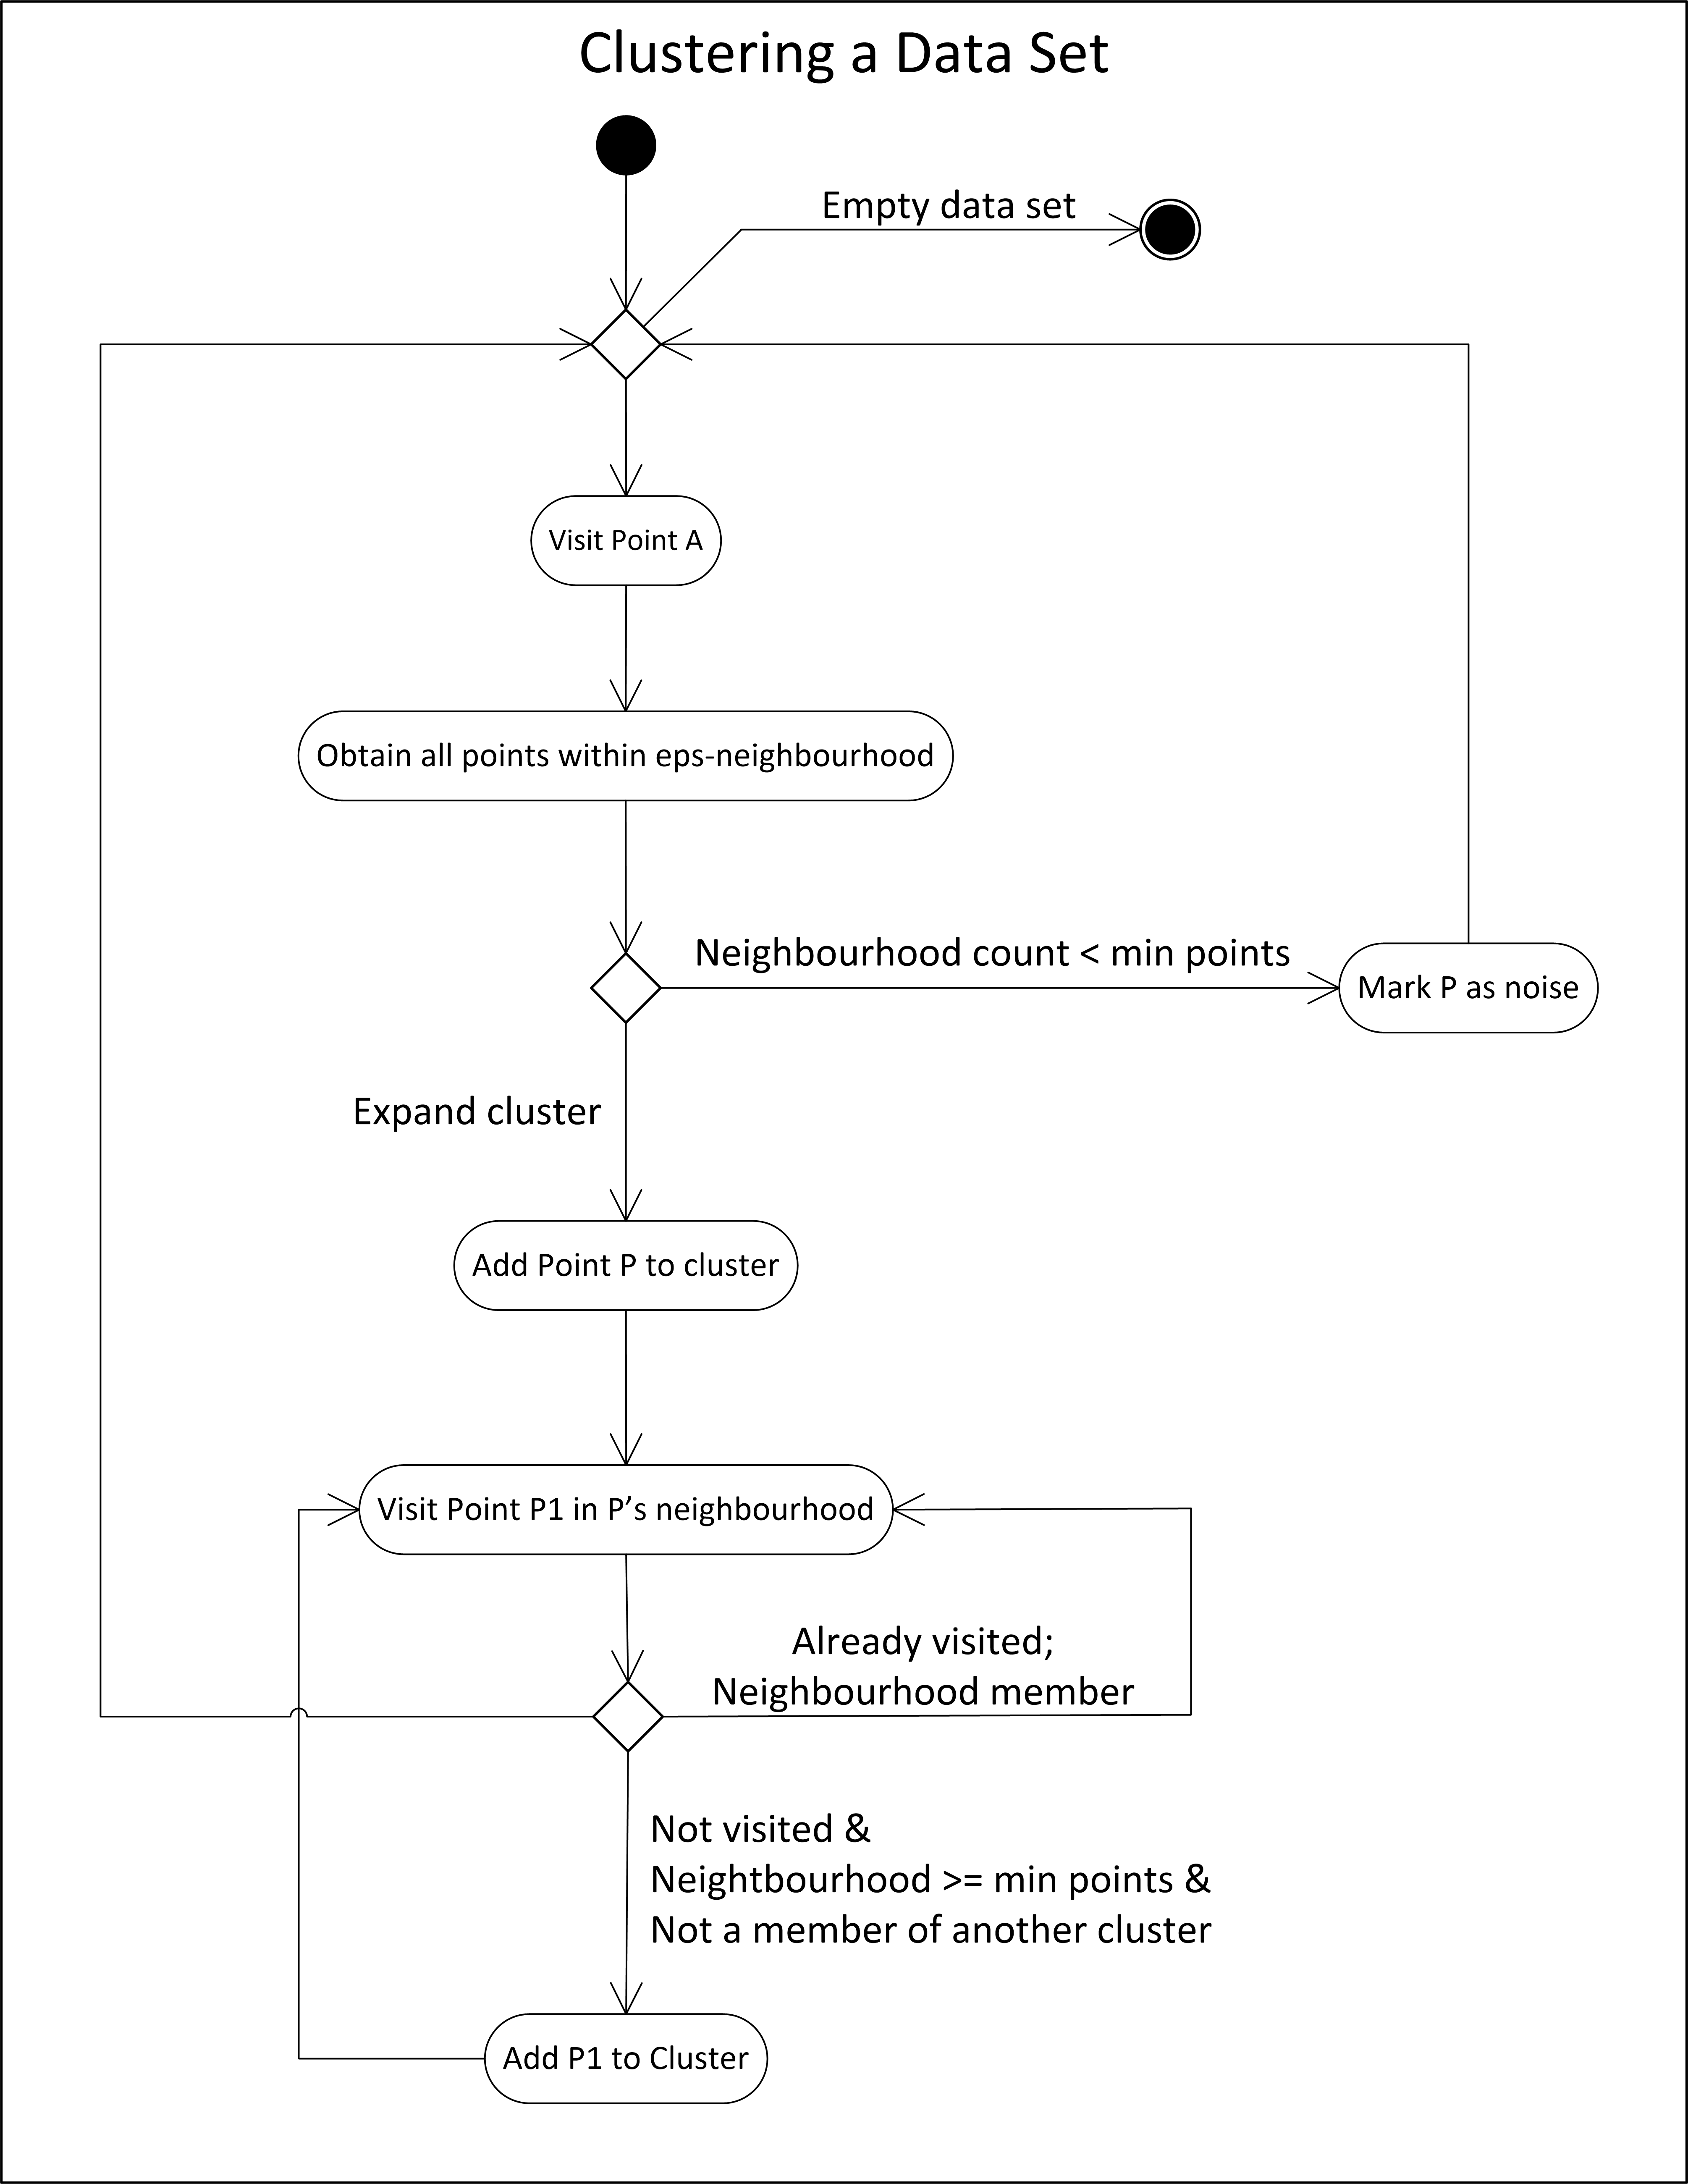
\includegraphics[scale=0.9]{chapter7/activity/clustering_data_set.png}
    \caption[Clustering a data set activity diagram]
            {An activity digram highlighting the various actions that are 
             required to be taken in order to cluster a set of data}
    \label{fig:clusterdataactivity}
\end{figure}



\subsection{Analysing a Cluster}
Figure \ref{fig:analyseclusteractivity} highlights the analysis of a cluster. 
This activity performs a number of business actions, that have been defined 
directly by BlackBerry. Identification of the cluster sizes, the similarities 
and differences form part of the first initial points to start to analyse the 
clusters.

Once completed, a more in depth analysis takes place. This in depth analysis 
looks at differences between the meta data (additional data associated with an 
Event), such as the RAT usage.

\begin{figure}[H]
  \centering
    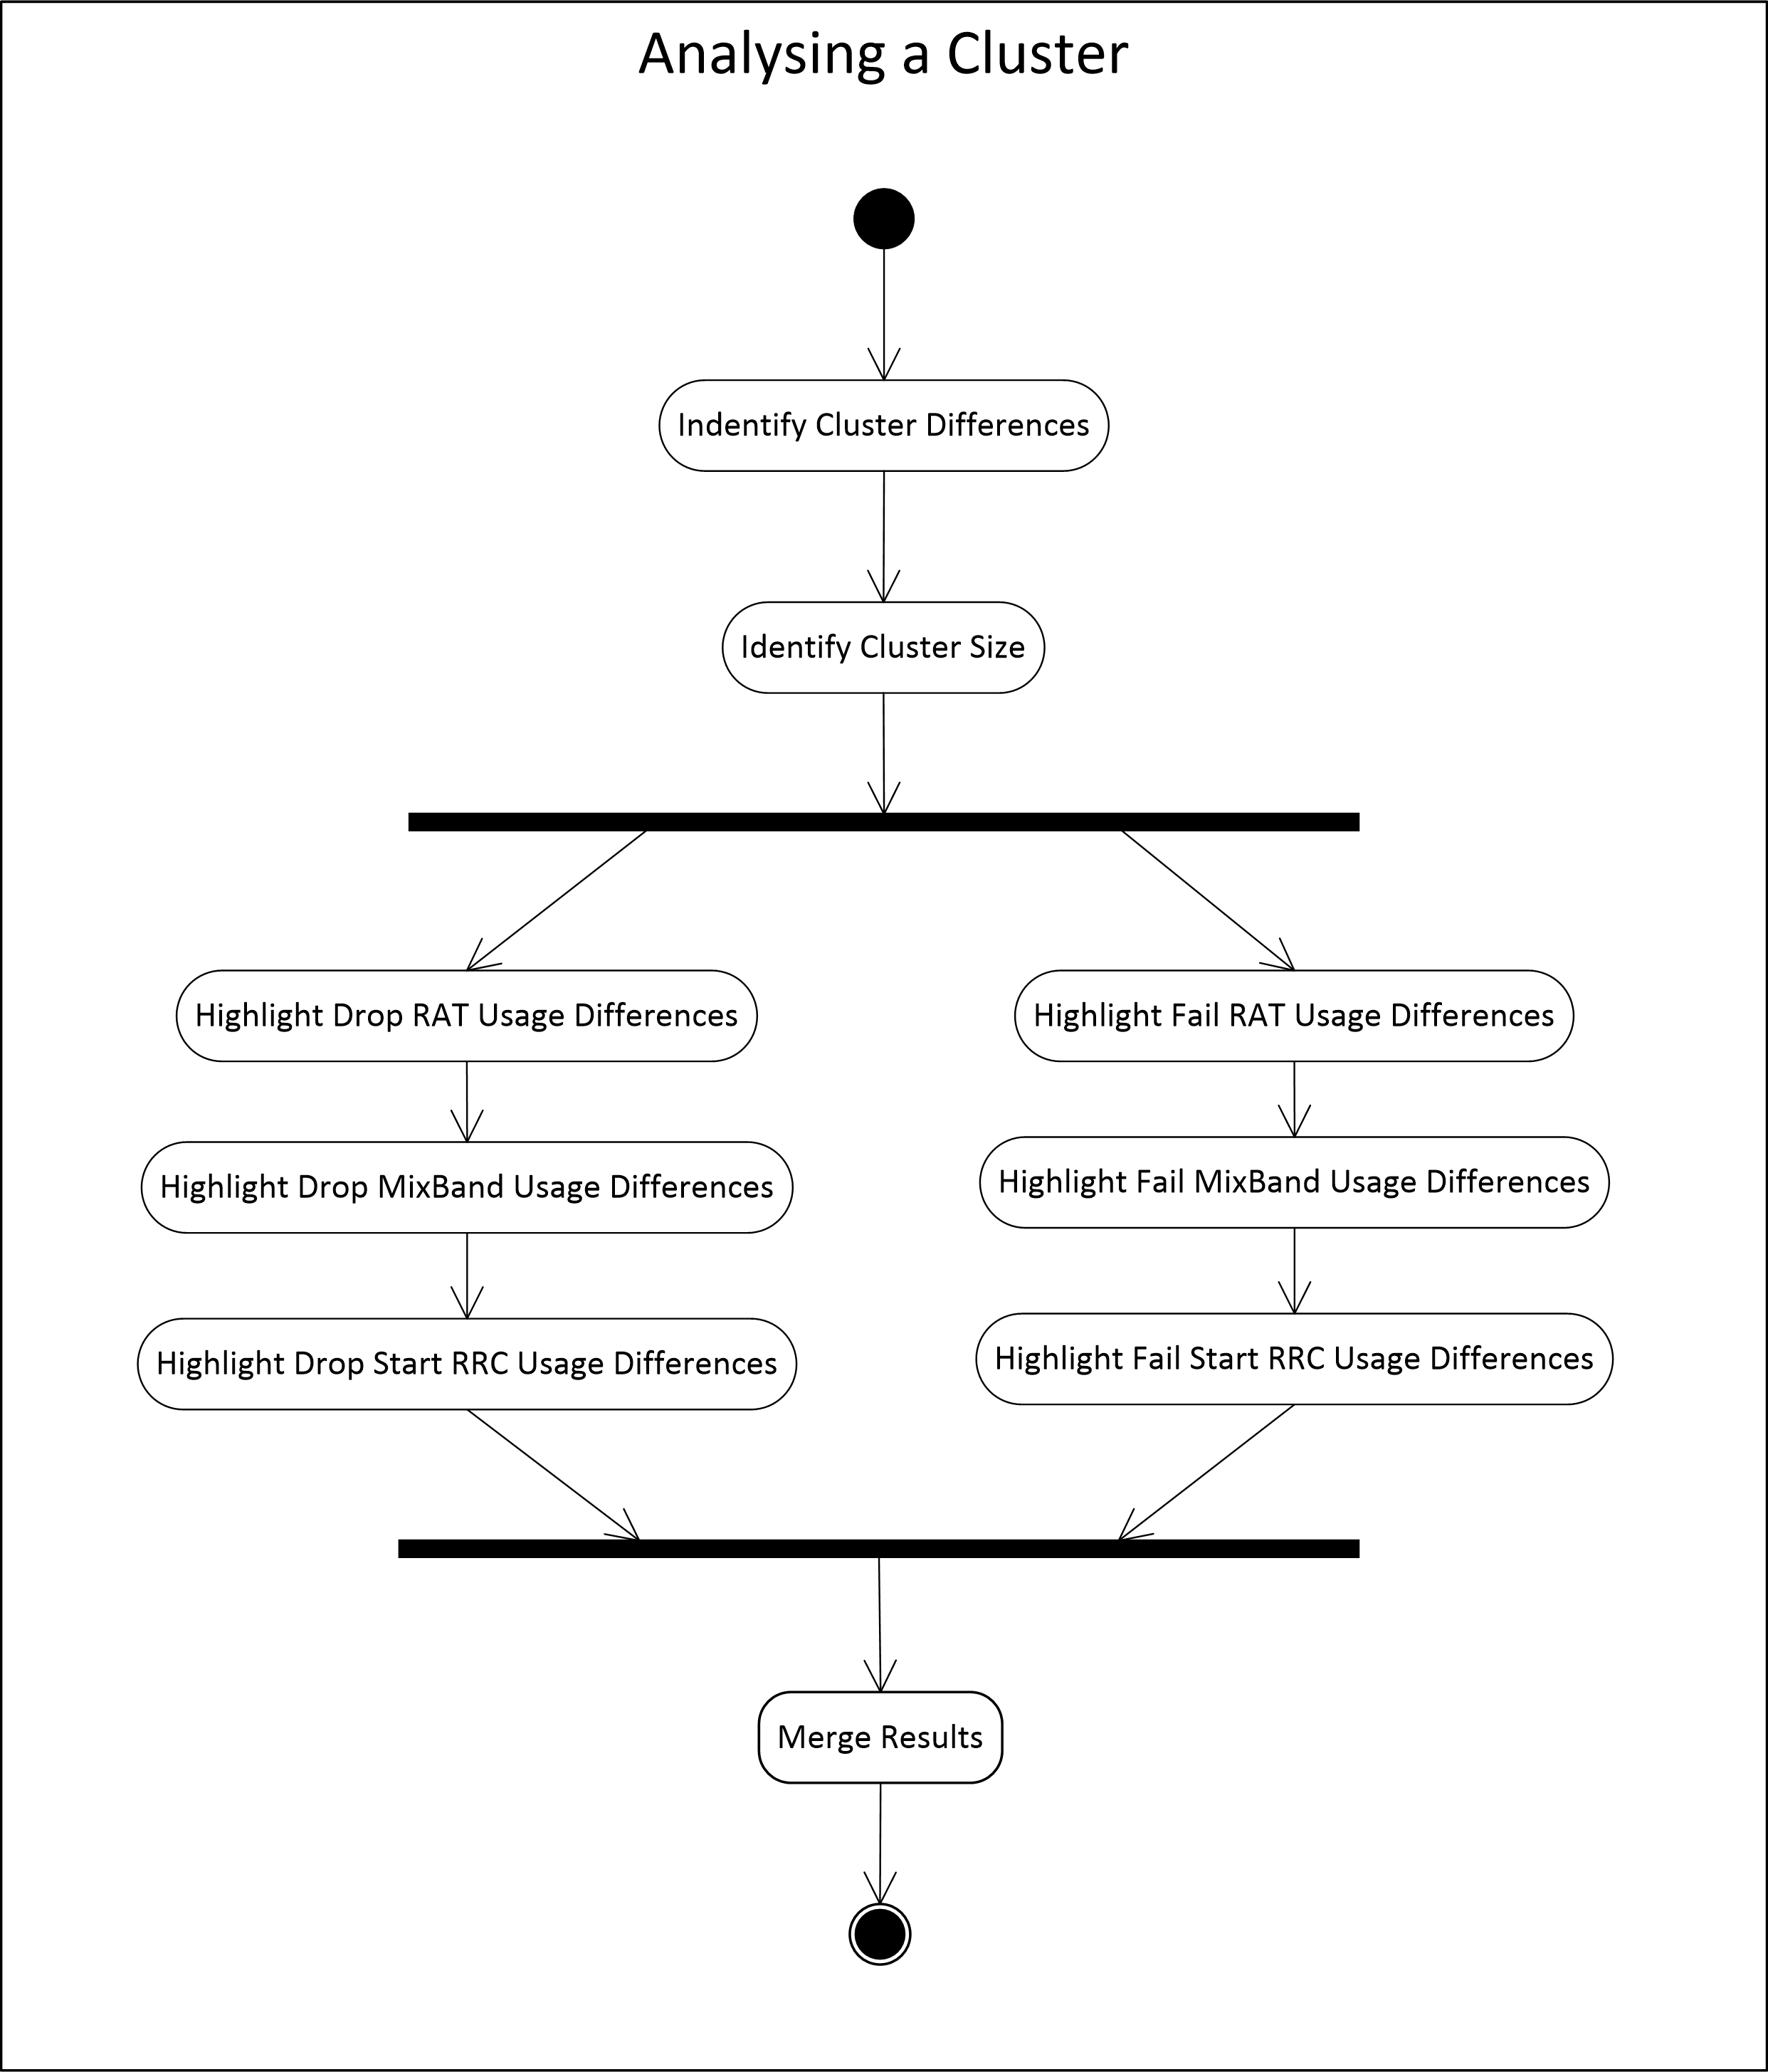
\includegraphics[scale=0.9]{chapter7/activity/analyse_cluster.png}
    \caption[Analysing a cluster activity diagram]
            {An activity digram highlighting the various actions that are 
             required to be taken in order analyse a clustered set of data}
    \label{fig:analyseclusteractivity}
\end{figure}


% Use Case Diagrams
\newpage
\section{Use Case Diagrams}

A Use Case diagram is ``a definition of a meaningful interaction with a 
computer system'' \citep{lunn03}. Use case diagrams are a powerful analysis 
technique. At the highest level they can easily define the presentation of a
system, whilst at the most detailed level can fully specify the external 
functionality of a system.

Within this section the use case of the entire system will be explored in 
detail. Figure \ref{fig:use_case} shows the use case for the entire system. 

To simplify the diagram, certain extensions and inclusions have been omitted. 
In the following sections these are discussed in more detail below.

\begin{figure}[H]
  \centering
    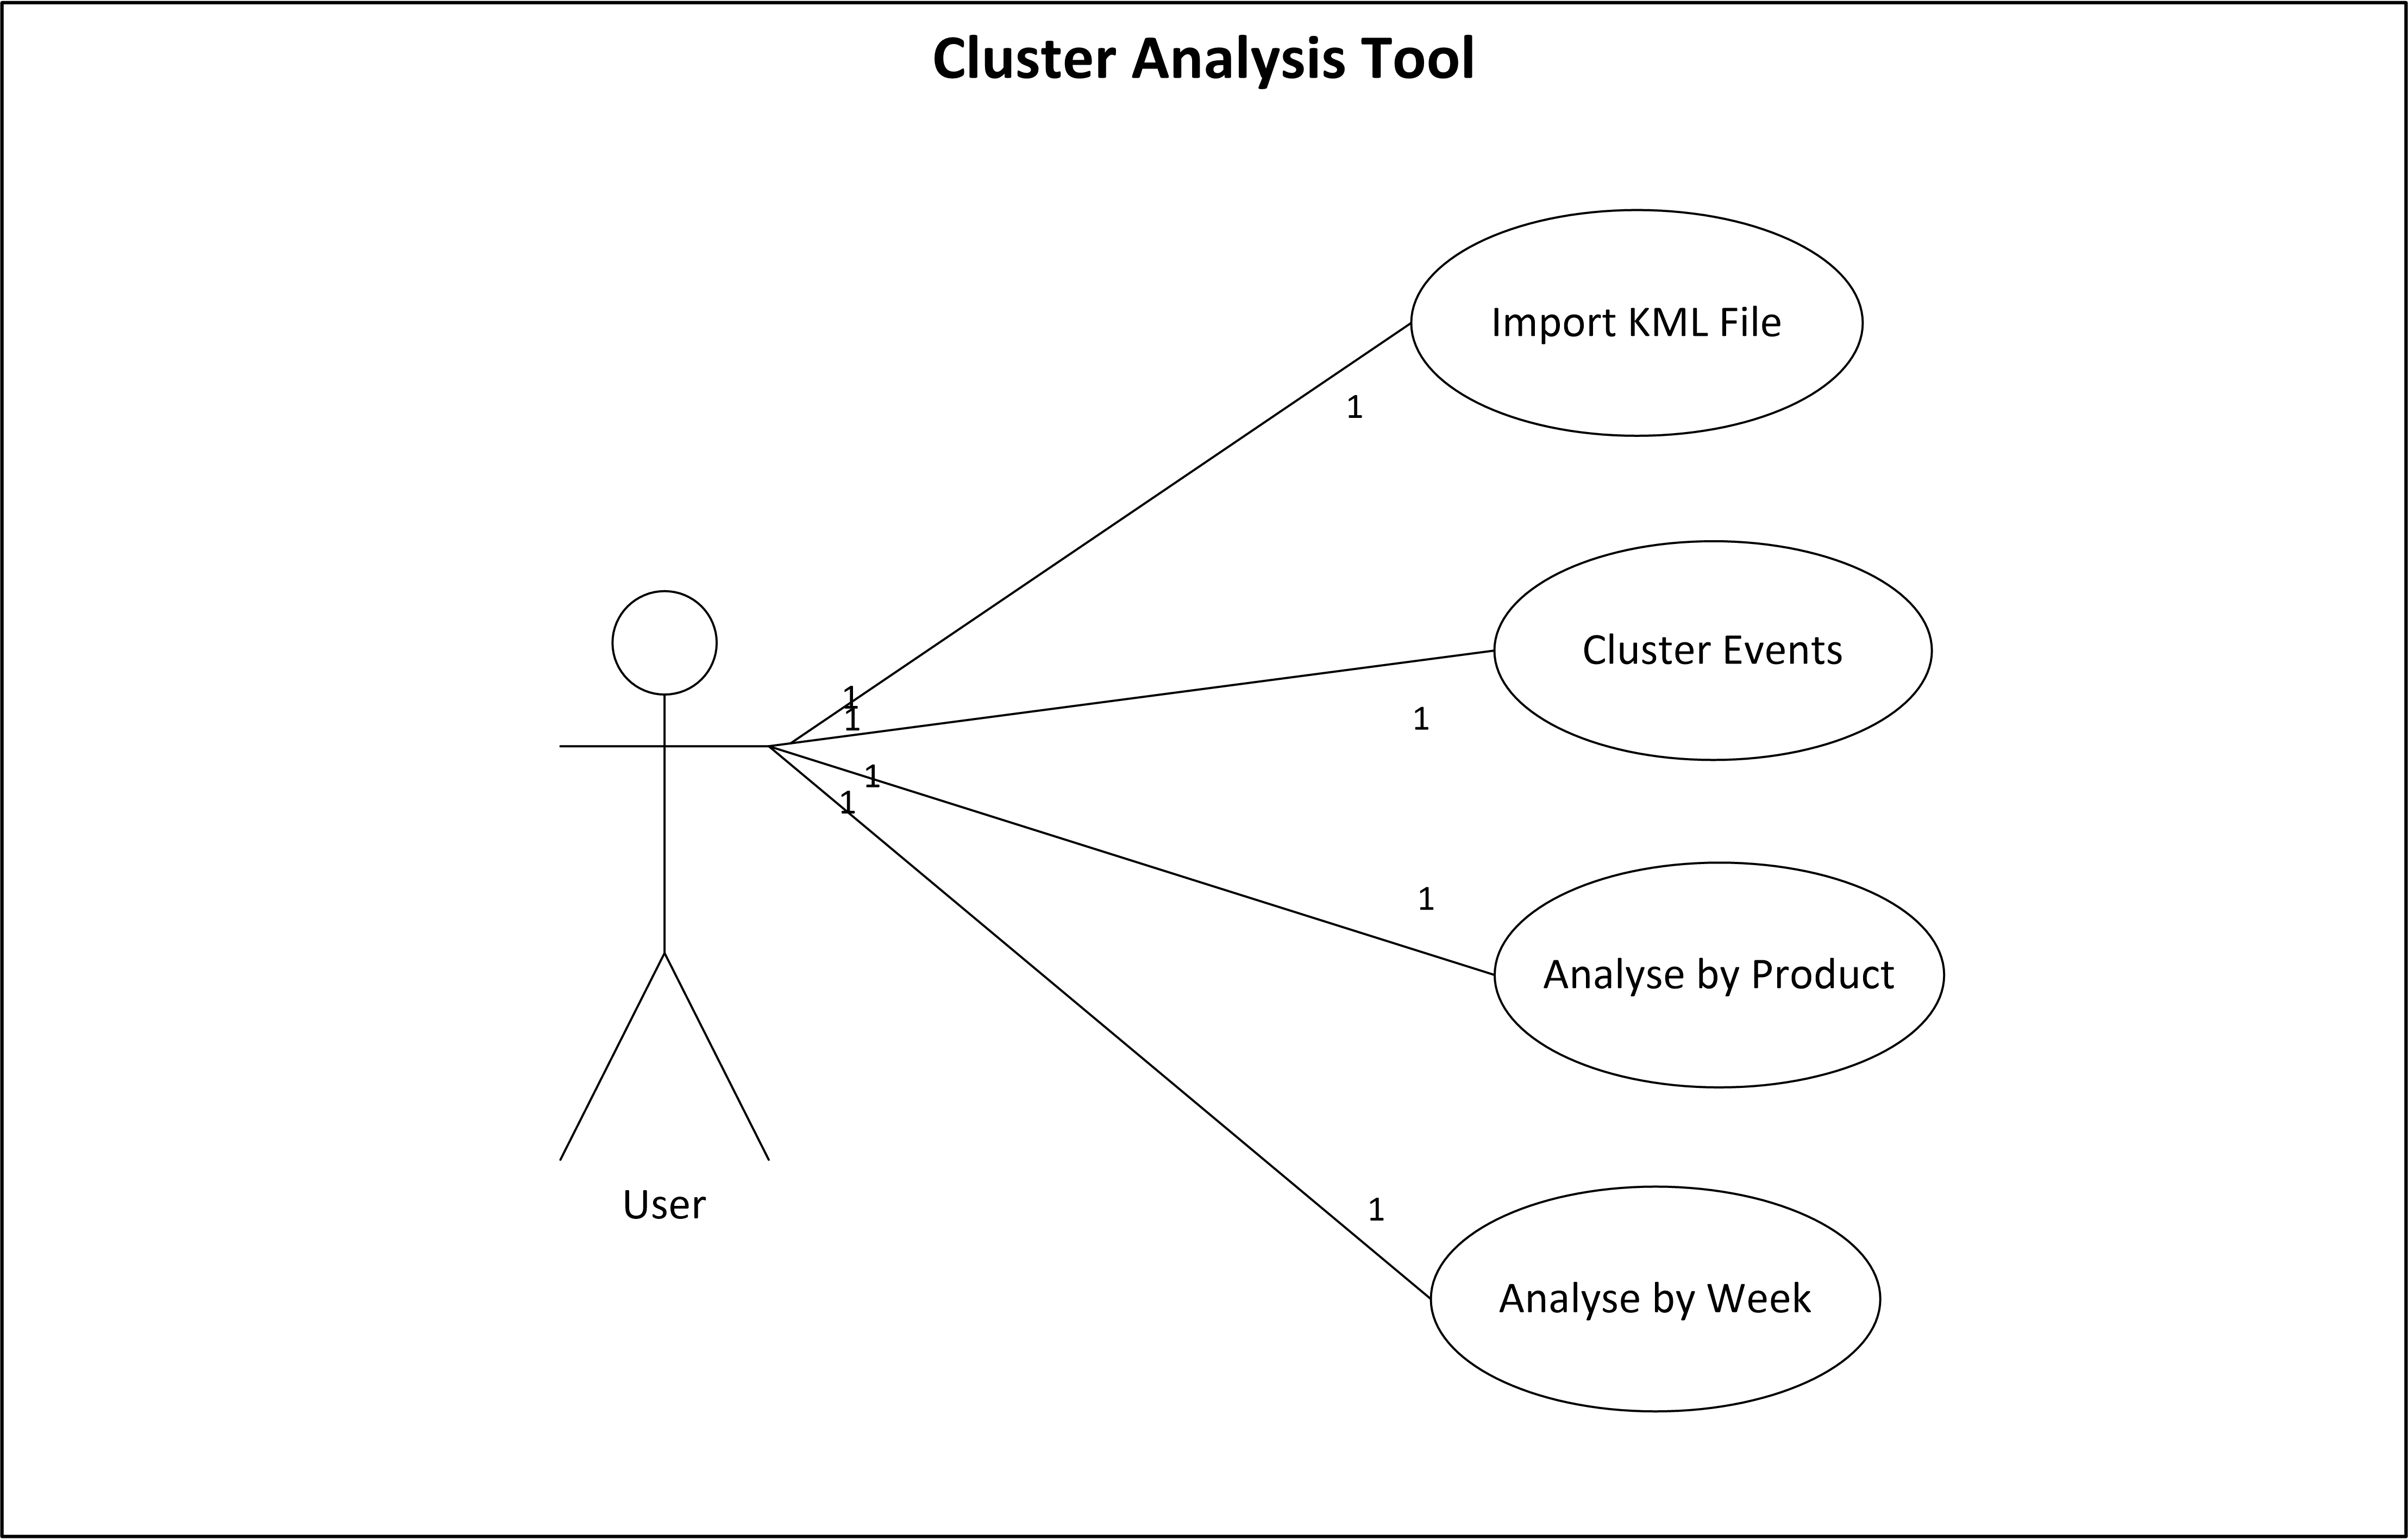
\includegraphics[scale=0.8]{chapter7/use_case/use_case.png}
    \caption[Use case diagram of the entire system]
            {Use case diagram of the entire system}
    \label{fig:use_case}
\end{figure}


\subsection{Importing Data}
Figure \ref{fig:UCImportData} highlights the use case for importing data into 
the system. The user is able to request that the tool imports either a single 
KML file or a directory containing multiple KML files.

The addition of this small option allows the end user to perhaps select various 
files that are stored across the file system. It also allows the user to point 
the tool directly at a directory that contains the required KML files.

Although integration with BlackBerry internal systems was originally a 
requirement that would not be implemented, this small addition does allow 
easier integration with any existing systems.

\begin{figure}[H]
  \centering
    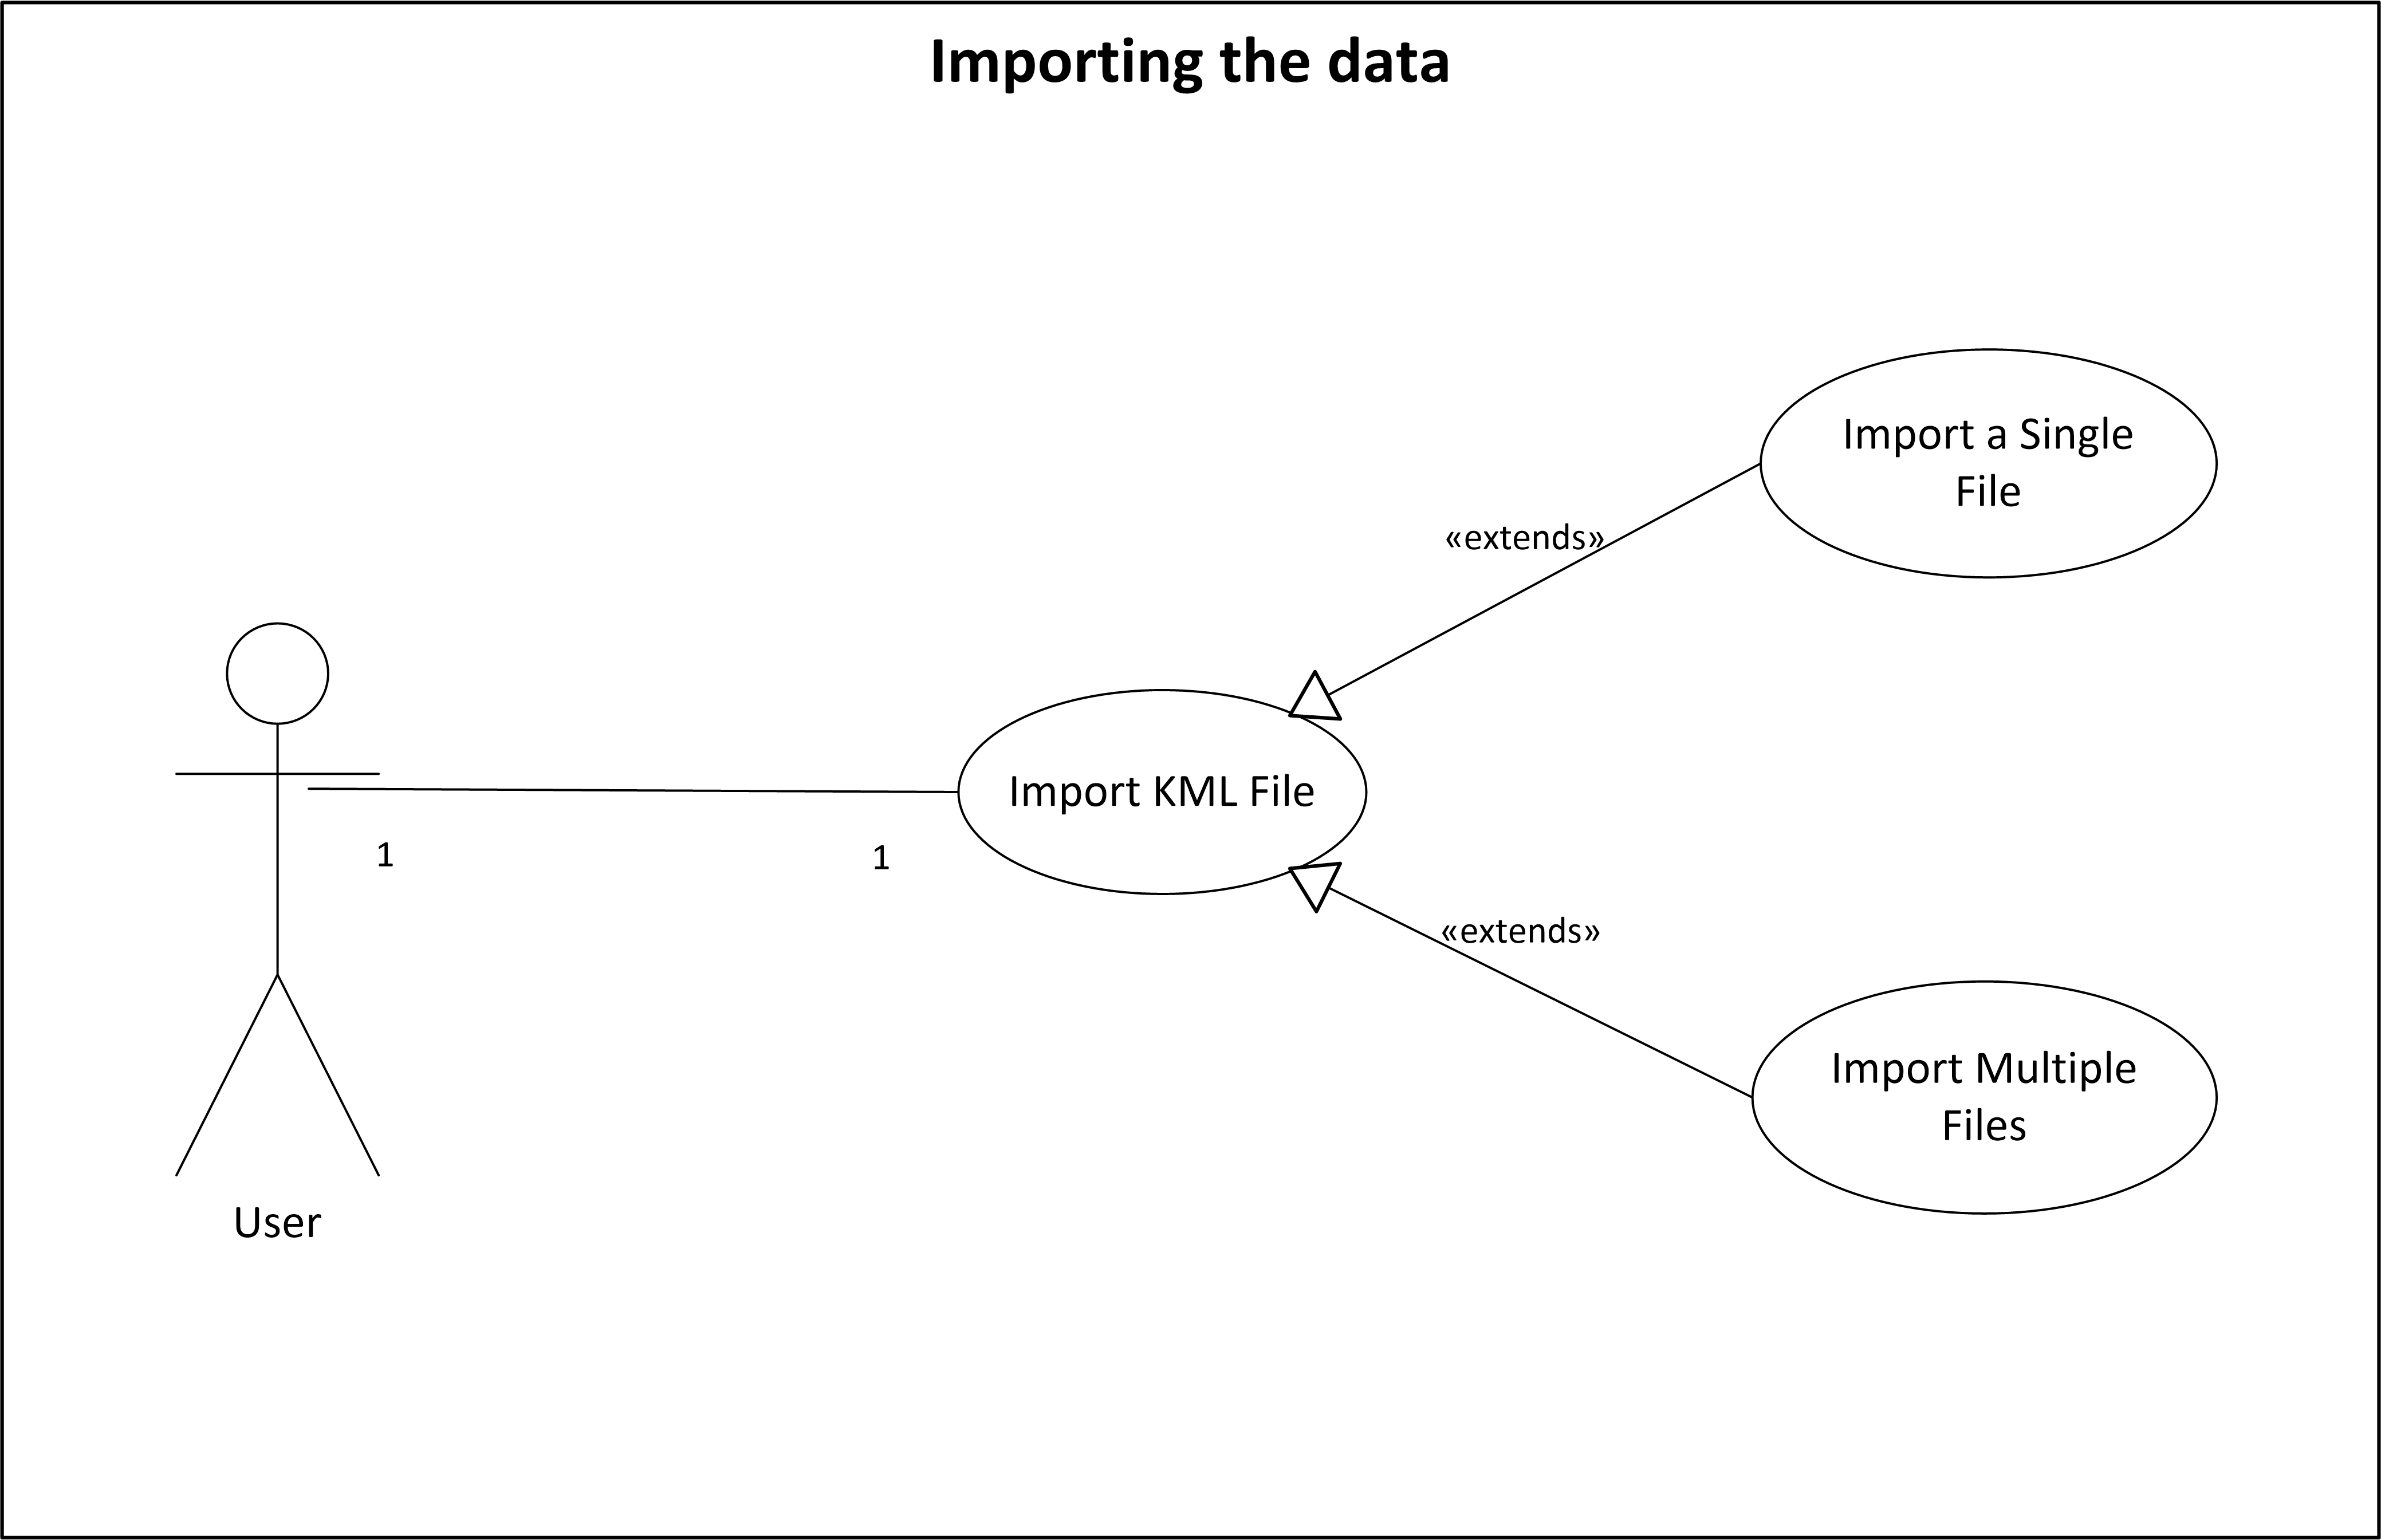
\includegraphics[scale=0.8]{chapter7/use_case/importing_data.png}
    \caption[Use case diagram to import KML data]
            {Use case diagram to import KML data}
    \label{fig:UCImportData}
\end{figure}


\subsection{Clustering}
Figure \ref{fig:UCClusterData} highlights the use case for clustering the data. 
In order to cluster, it is assumed that the user has already given a set of 
data to the algorithm.

The clustering mechanism utilises the DBSCAN algorithm, and requires two 
additional parameters in order to complete the clustering process. 

Firstly the algorithm will require a minimum number of points. This is the 
minimum number of points (or objects) required to form a cluster. This value 
must be set by the user, otherwise a default value will be used.

Secondly the algorithm will require the {\em EPS} value. The {\em EPS} 
(epsilon) value is the maximum distance allowed between two points (or objects)
to form a cluster.

\begin{figure}[H]
  \centering
    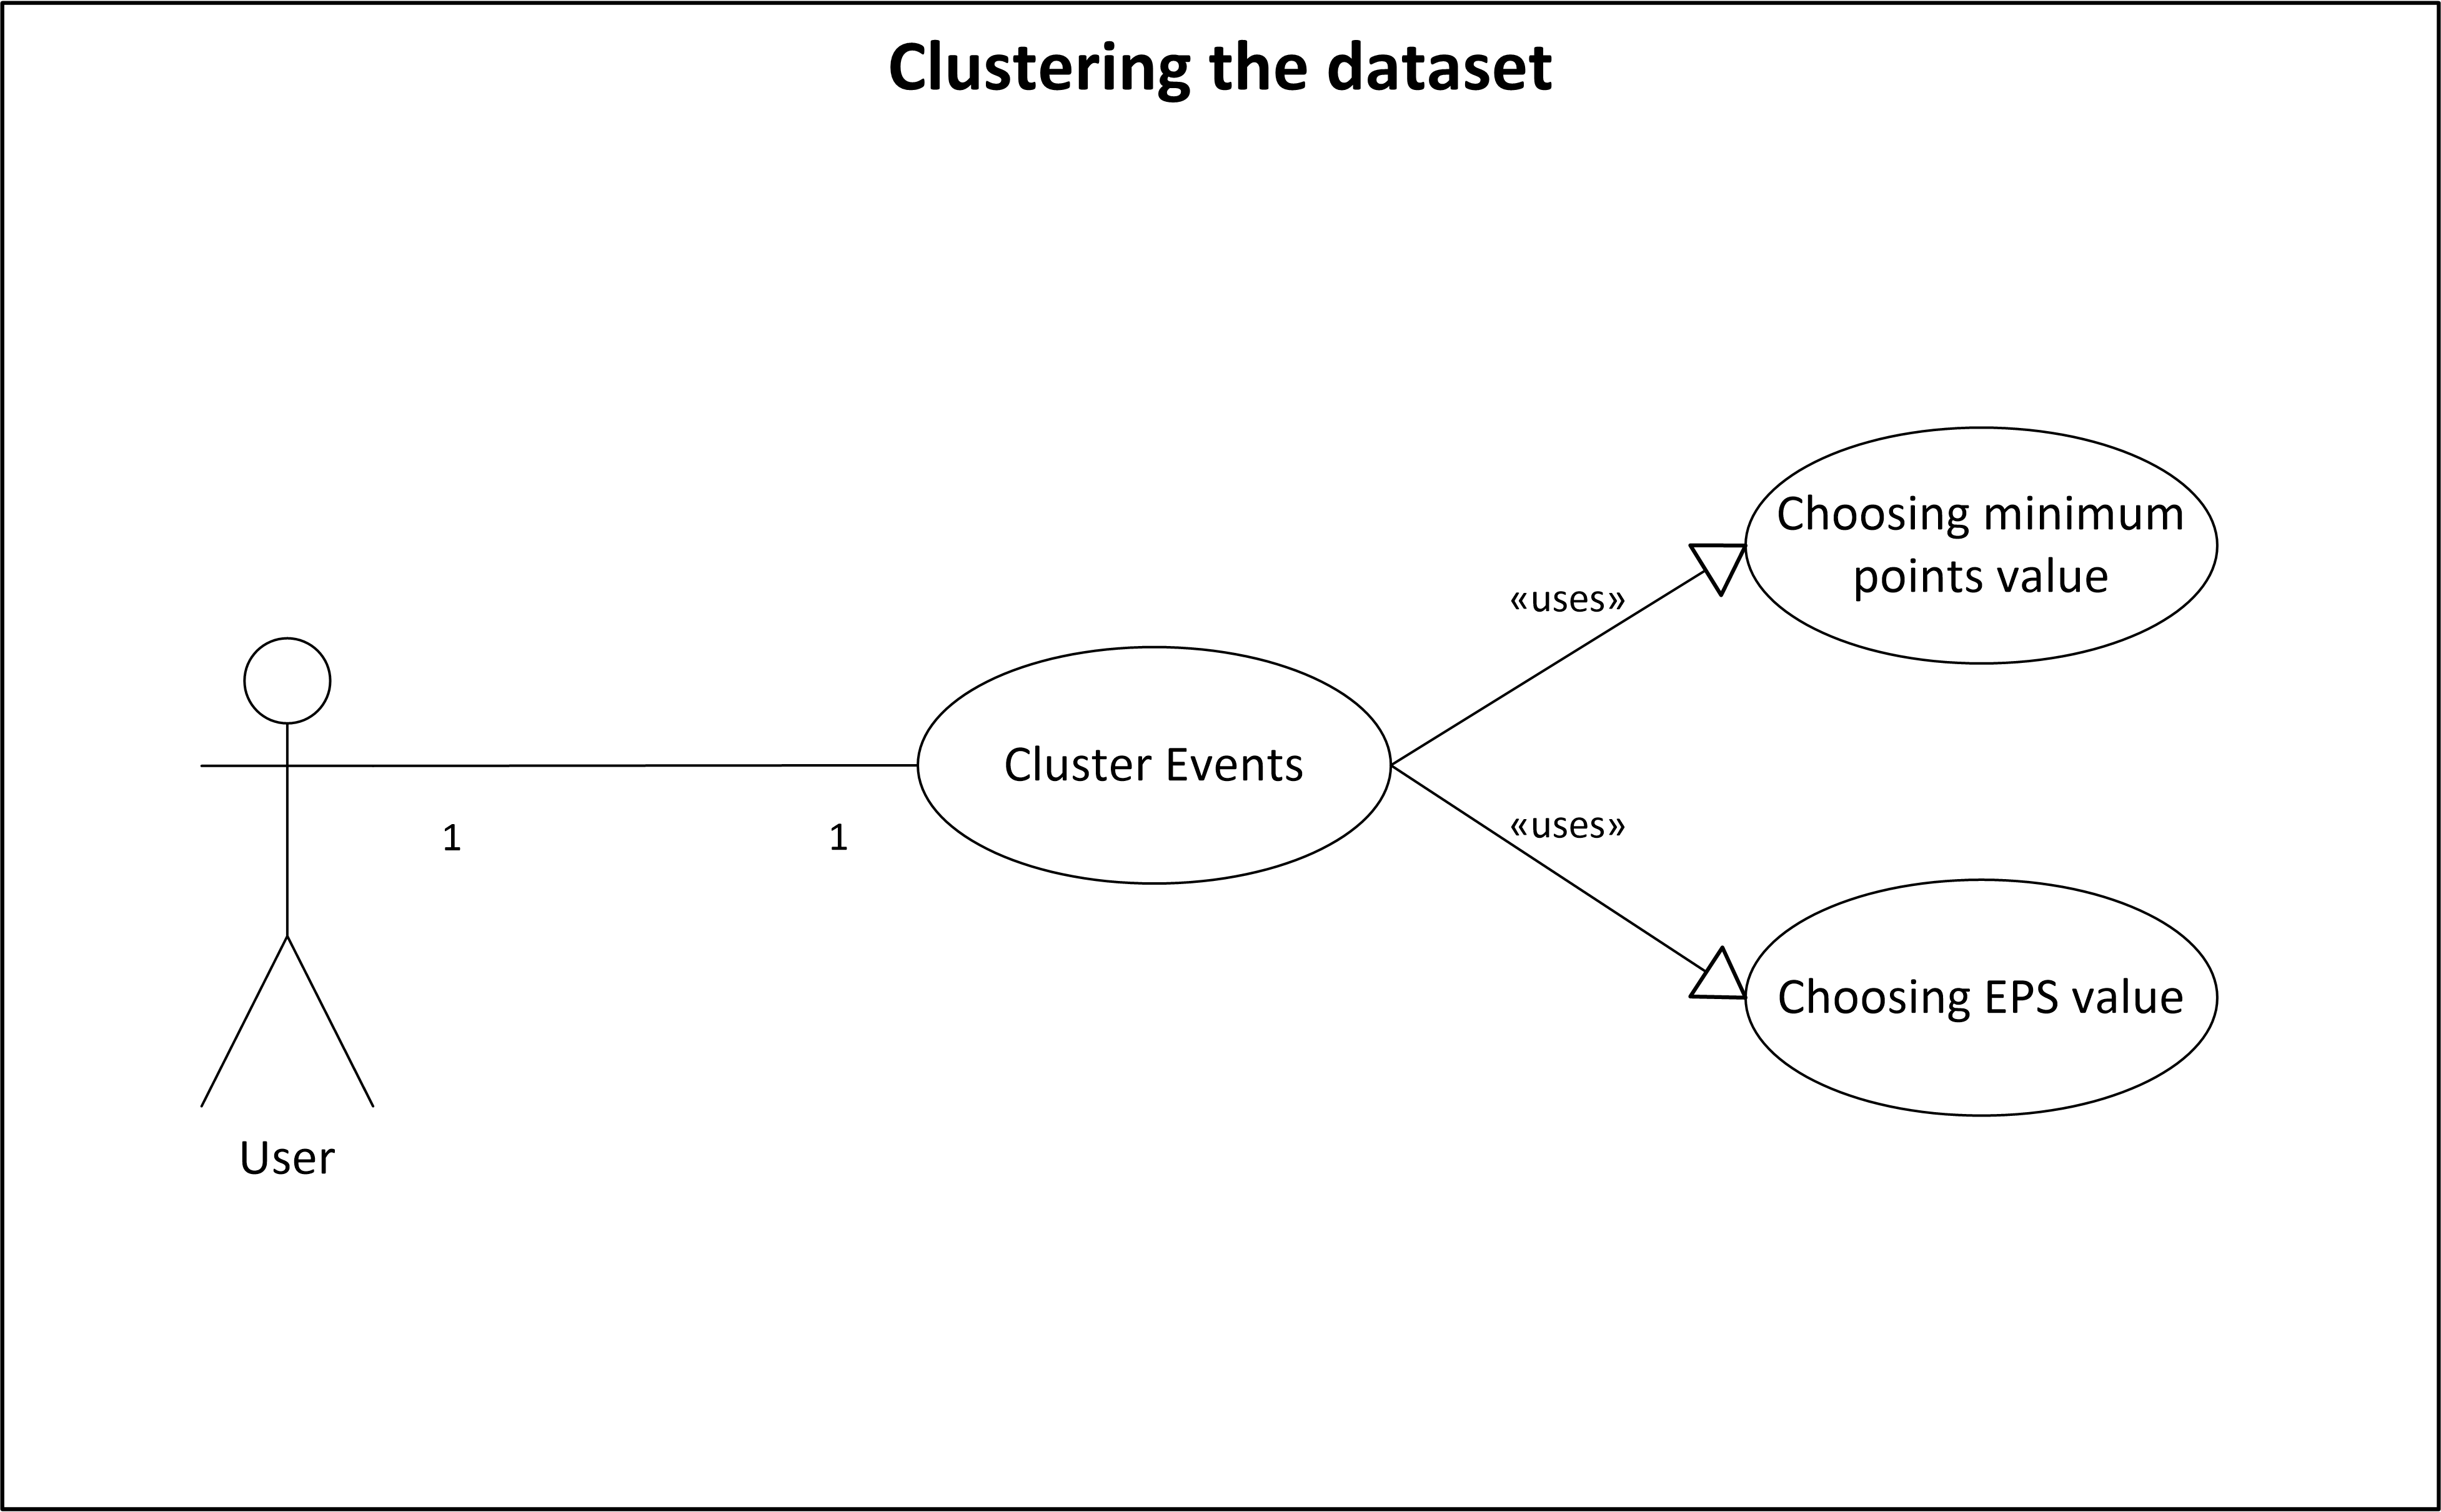
\includegraphics[scale=0.9]{chapter7/use_case/cluster_data.png}
    \caption[Use case diagram highlighting data clustering]
            {Use case diagram highlighting data clustering}
    \label{fig:UCClusterData}
\end{figure}


\subsection{Results Analysis}
Figure \ref{fig:UCAnalyseData} highlights the use case for analysing the 
clustered data. Fundamentally, the analysis of clusters can take two distinct 
paths. Analysis can happen upon a Weekly basis or a Product basis.

Regardless of whichever fundamental route was taken, the back end analysis is 
the same. Firstly the user could create a number of charts that highlights the 
differences in RAT, Mix-Band and Start RRC state usages, as well as cluster 
sizes.

Secondly, the user could create a KML file, that is able to be view from within
Google Earth. This would show each cluster upon a map, along with a heat map to 
highlight the cluster intensities.

Finally use user could choose to create a number of charts, and create an 
output KML file --- i.e. perform both of the previous options.

\begin{figure}[H]
  \centering
    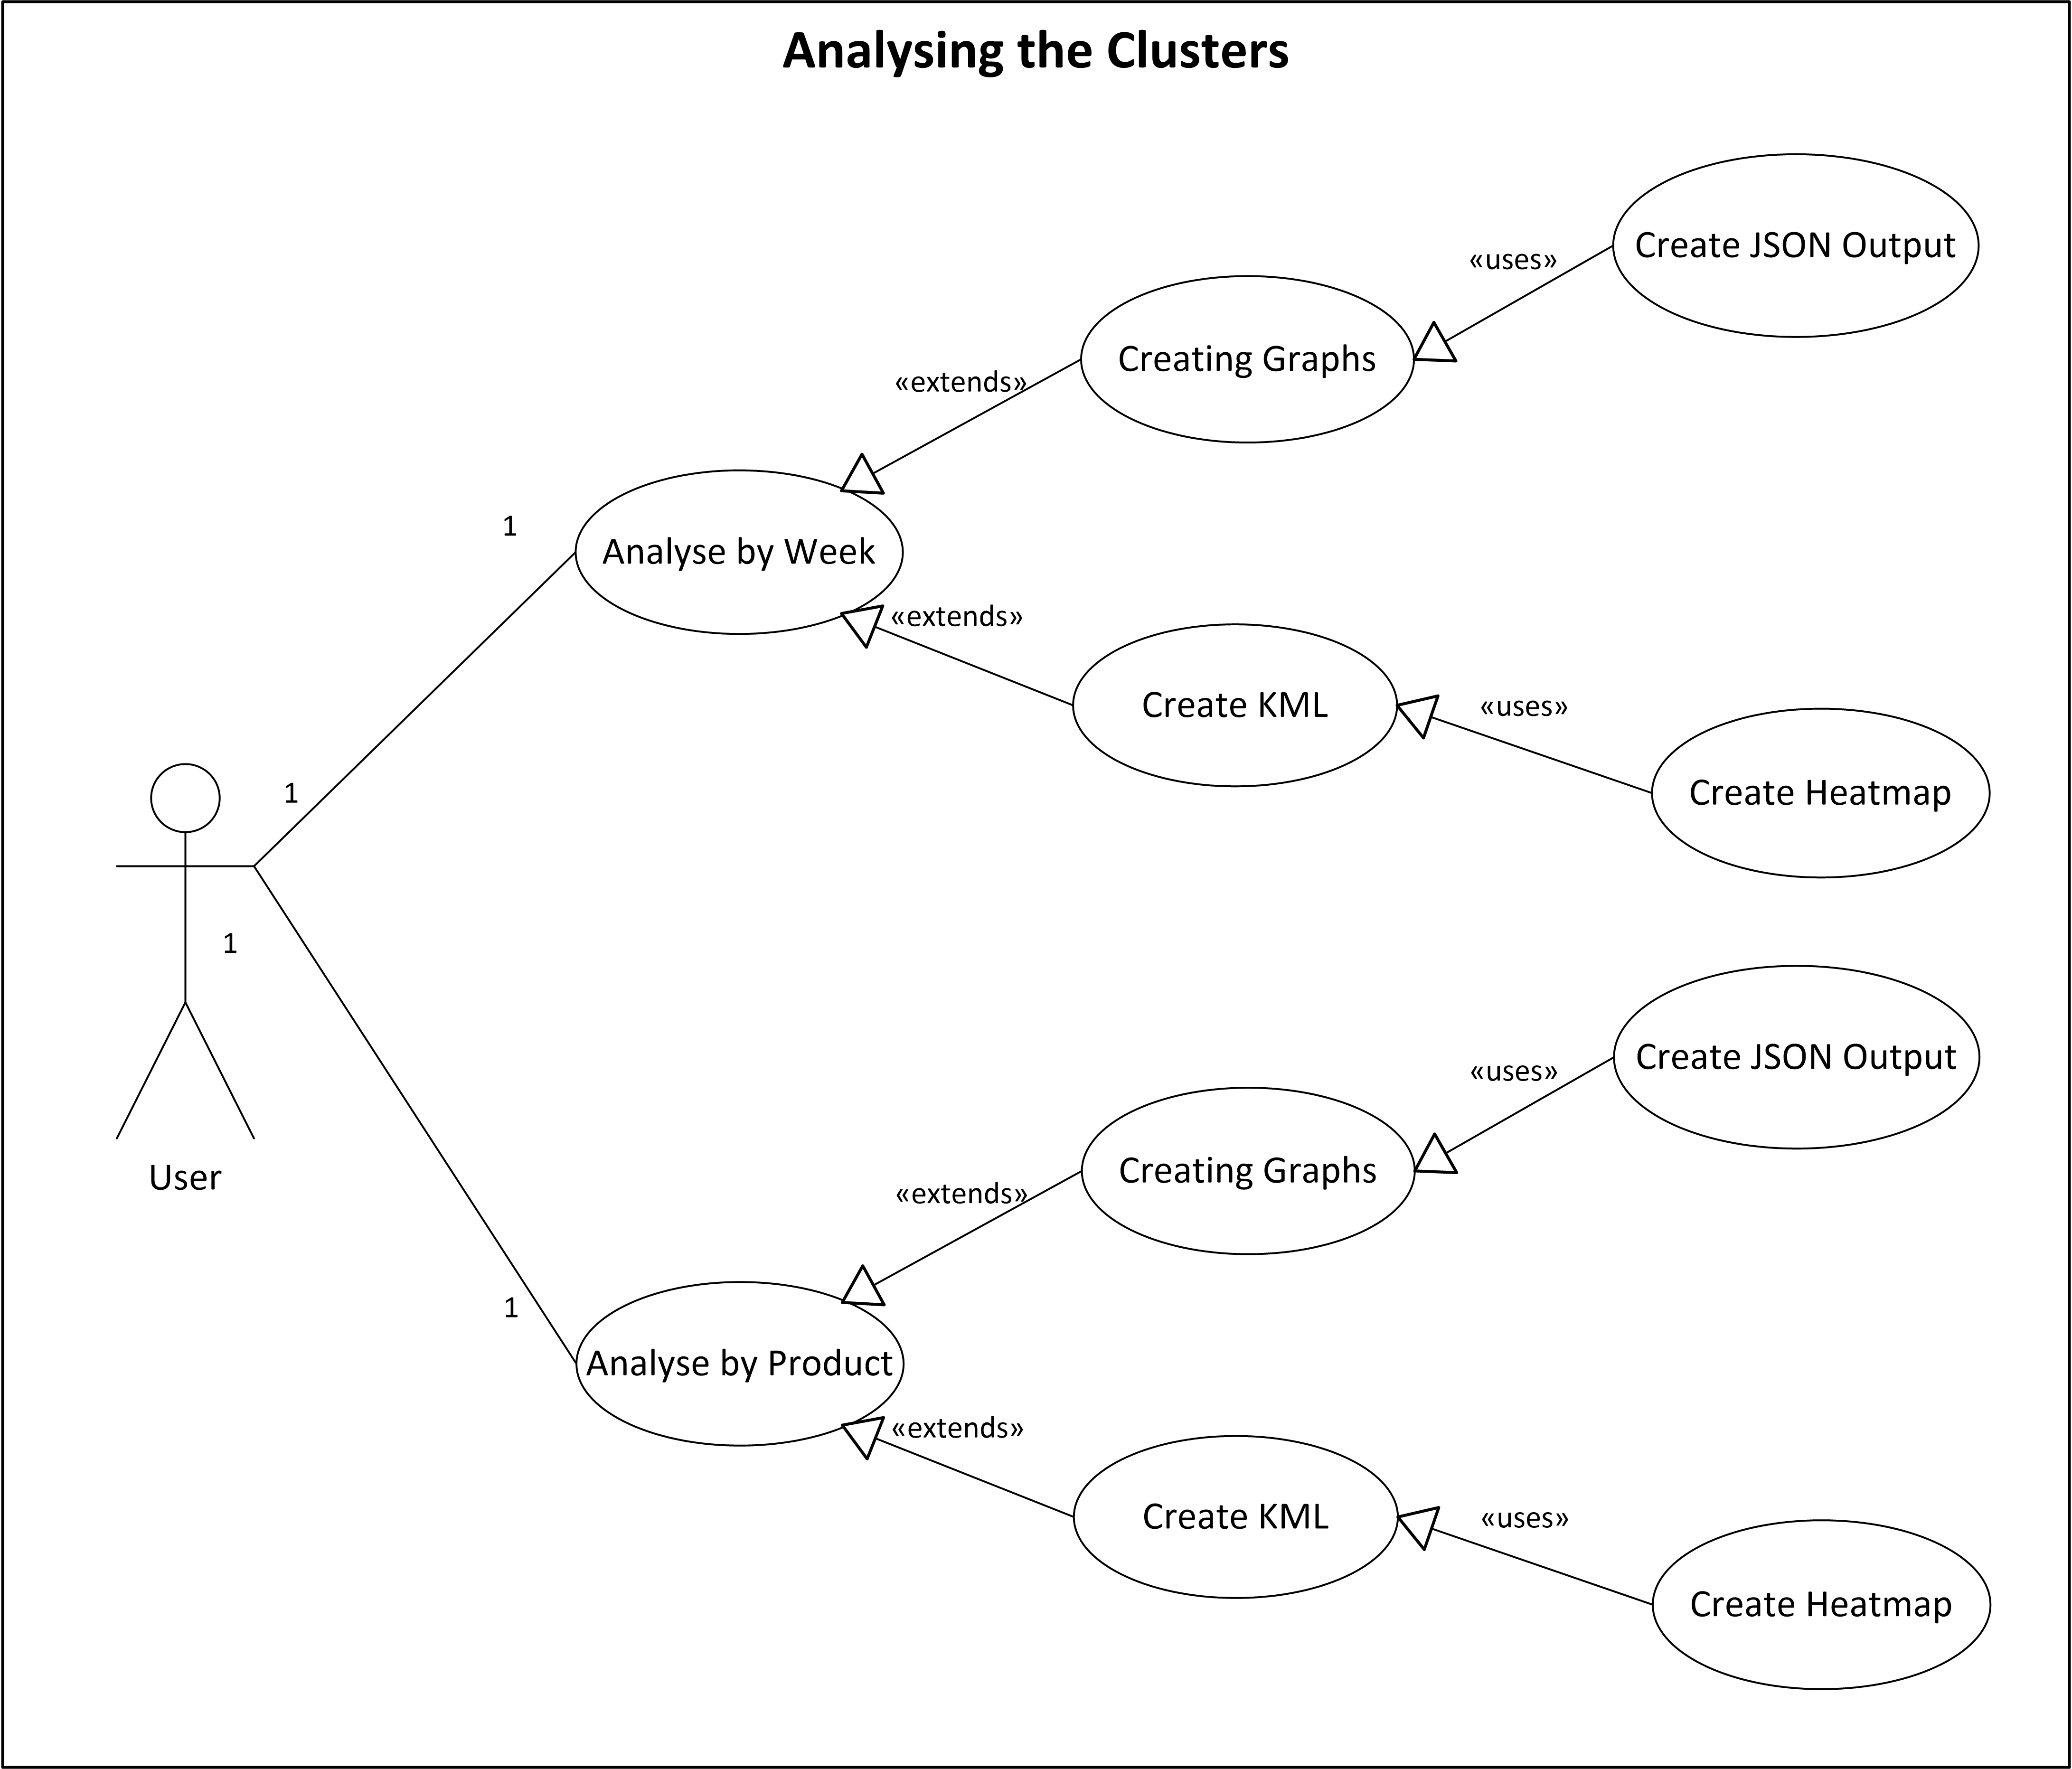
\includegraphics[scale=0.8]{chapter7/use_case/analyse_results.png}
    \caption[Use case diagram highlighting importing data]
            {Use case diagram highlighting importing data}
    \label{fig:UCAnalyseData}
\end{figure}


% Sequence Diagrams
\newpage
\section{Sequence Diagrams}

The previous section outlined the functions of the system. Each of these 
functions are now to be ``converted'' into set of objects and interactions that 
might be implemented. A sequence diagram is ``one way of describing a journey 
through a system'' \citep{lunn03}.

\subsection{Single Week Cluster and Analysis (Weekly Basis)}
Figure \ref{fig:singleweekly} highlights the sequence of events that make up 
the clustering of data and analysing the clusters upon a weekly basis. This 
sequence diagram assumes that only one KML file will be given. 

Once clustered, the analysis only would be required to highlight the usage 
differences for the clusters that had been previously formed. An example of 
usage differences could be the number of events that occurred in one cluster 
versus another cluster, such as the number of 3G drops. 

Obviously as this is only a single week analysis then comparisons to other 
week's clusters can not be made.

Once the analysis has been completed, the results are written to a Javascript 
Object Notation (JSON) file and a new output KML file. This process was 
described in figure \ref{fig:UCAnalyseData}.

% Landscape page
\begin{landscape}
  % Center image
  \centering 
  \begin{figure}
    \centering
      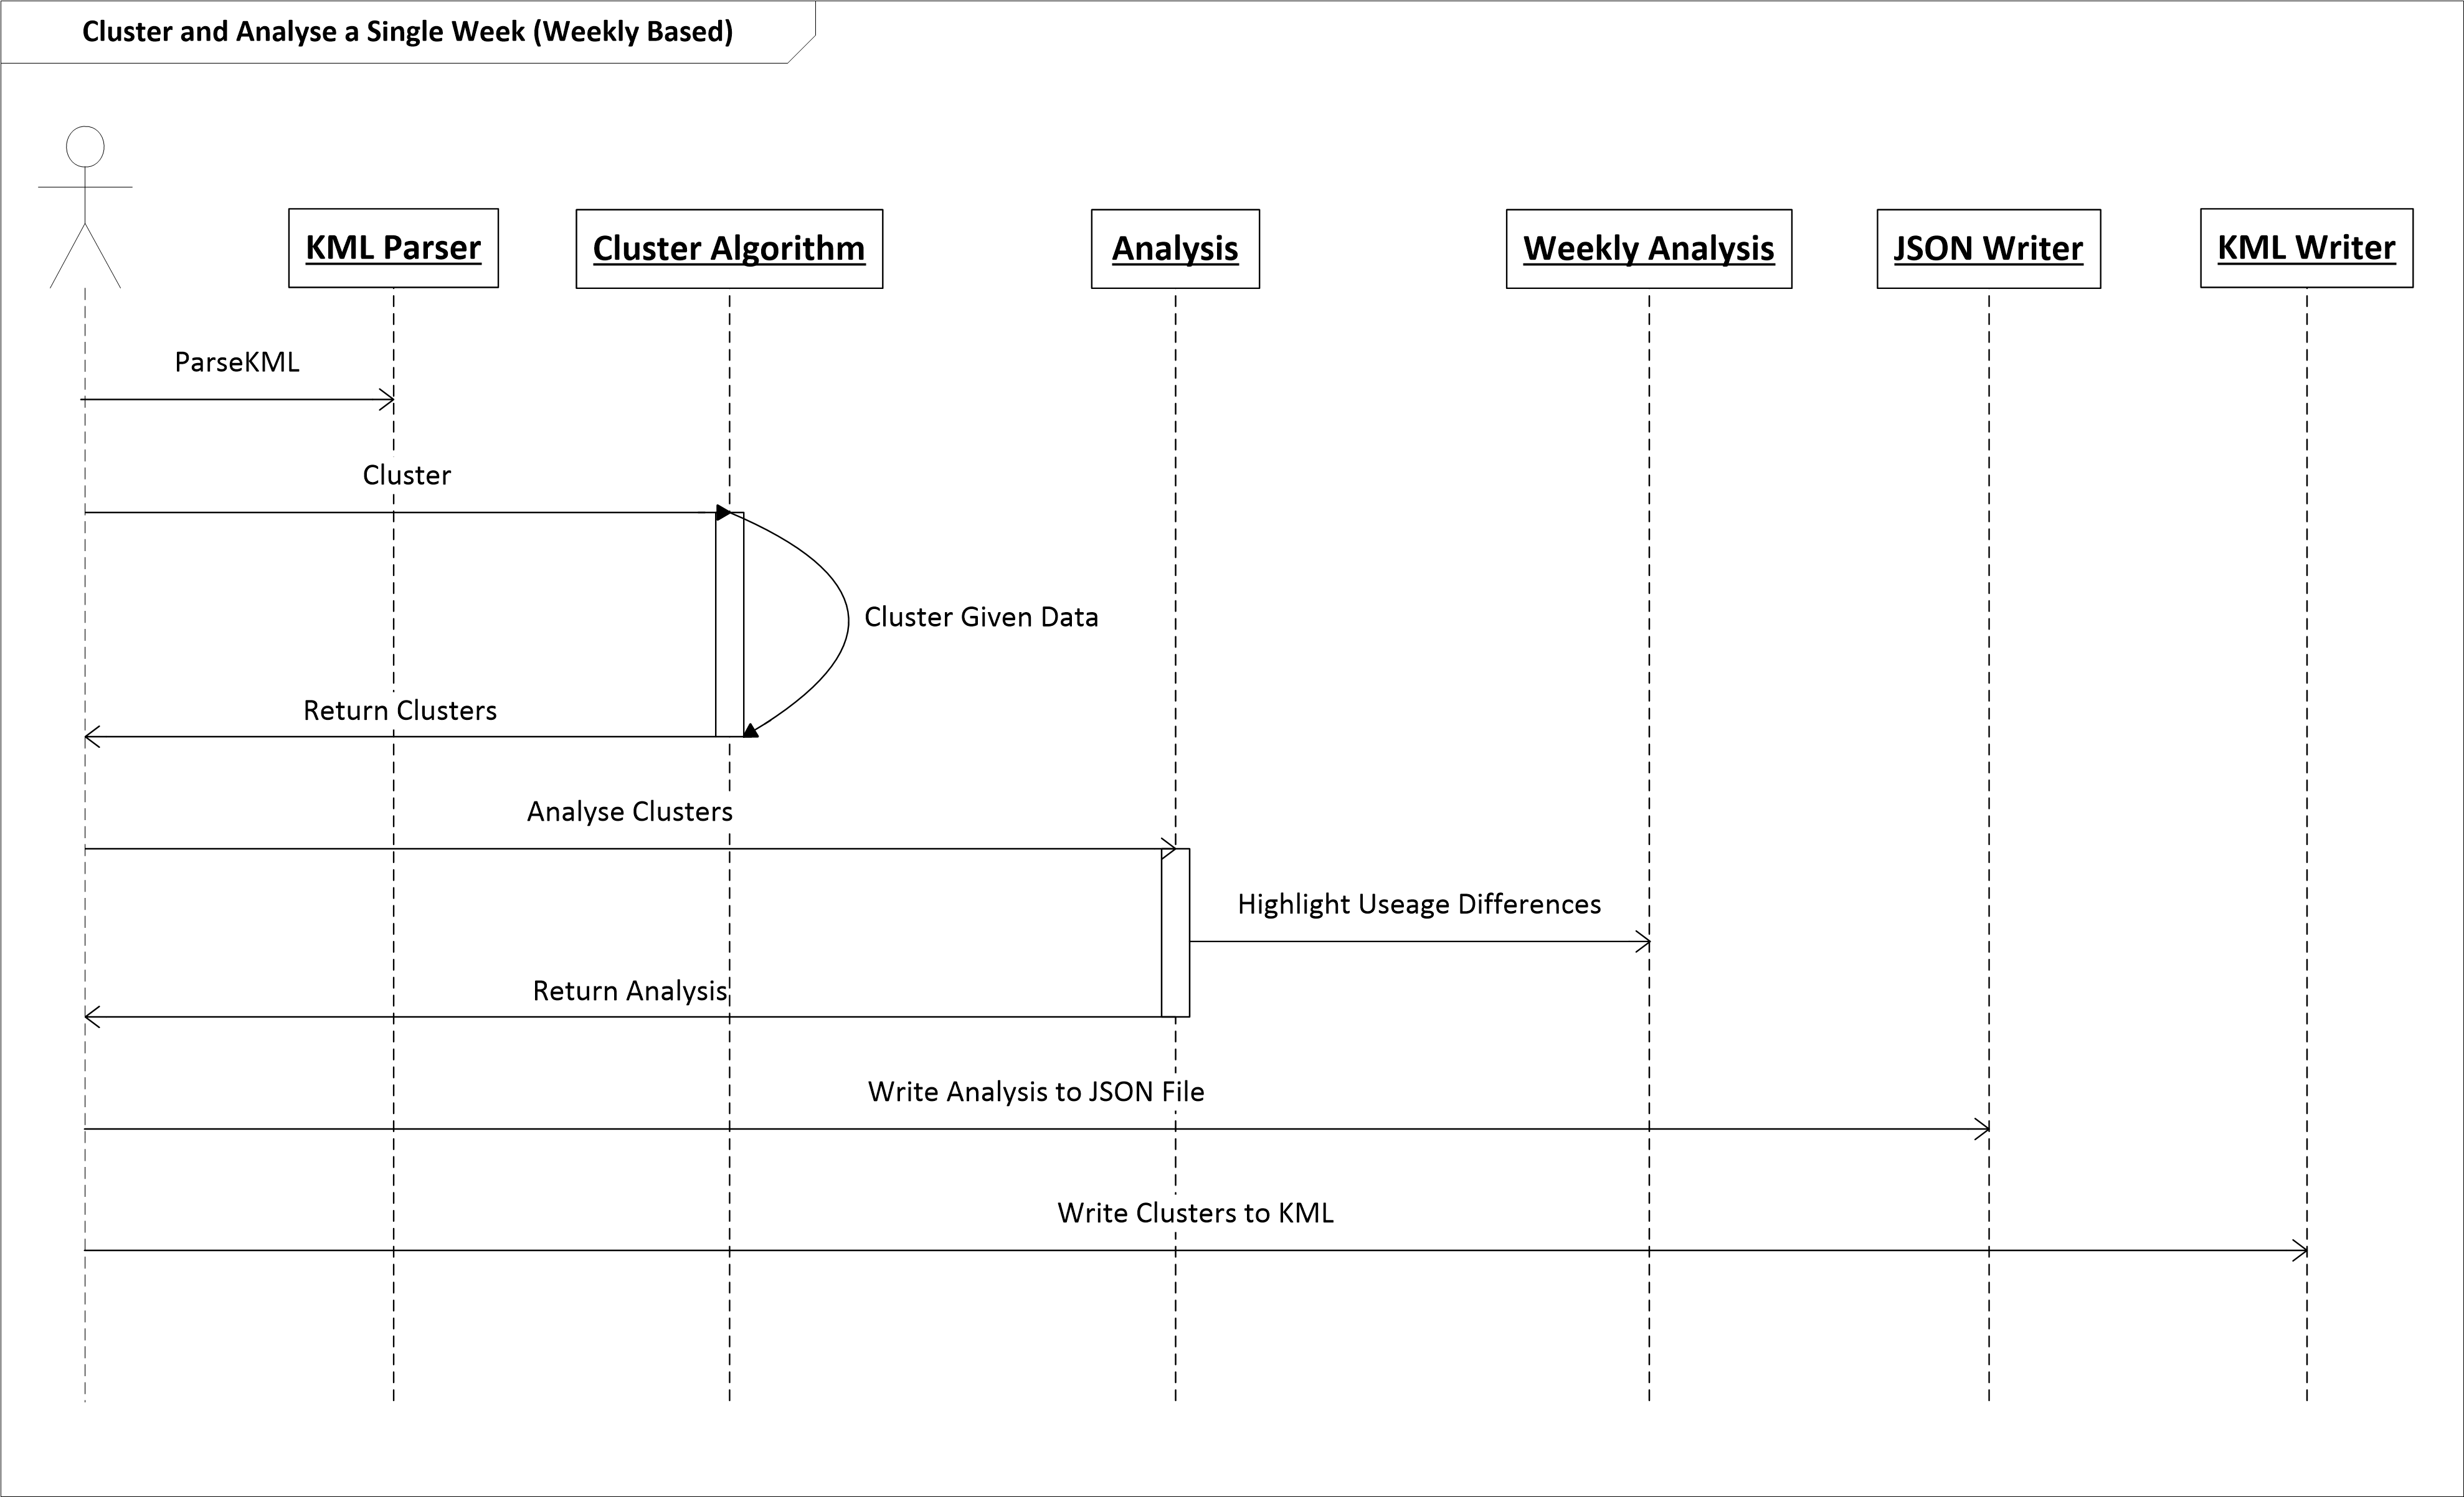
\includegraphics[scale=0.8]{chapter7/sequence_diagrams/single_week_cluster_weekly.png}
      \caption[Sequence diagram of a single week being clustered]
              {Sequence diagram of a single week being clustered and analysed 
              upon a weekly basis.}
      \label{fig:singleweekly}
  \end{figure}
\end{landscape}


\newpage
\subsection{Single Week Cluster and Analysis (Product Basis)}
Figure \ref{fig:singleproduct} highlights the sequence of events that make up 
the clustering of data and analysing the clusters upon a product basis.

As with the previous diagram, the tool would only be required to highlight the 
usage differences for the clusters that had been previously formed. However upon 
closer inspection, the Analysis event interacts with a `Product Analysis' event 
rather than the `Weekly Analysis' event that was found within the last diagram.

This highlights the only difference in the sequence of events for the weekly 
based analysis and the product based analysis.

As previously mentioned, once the analysis has been completed, the results are 
written to a JSON file and a new output KML file (see figure 
\ref{fig:UCAnalyseData} for more details).

% Landscape page
\begin{landscape}
  % Center image
  \centering 
  \begin{figure}
    \centering
      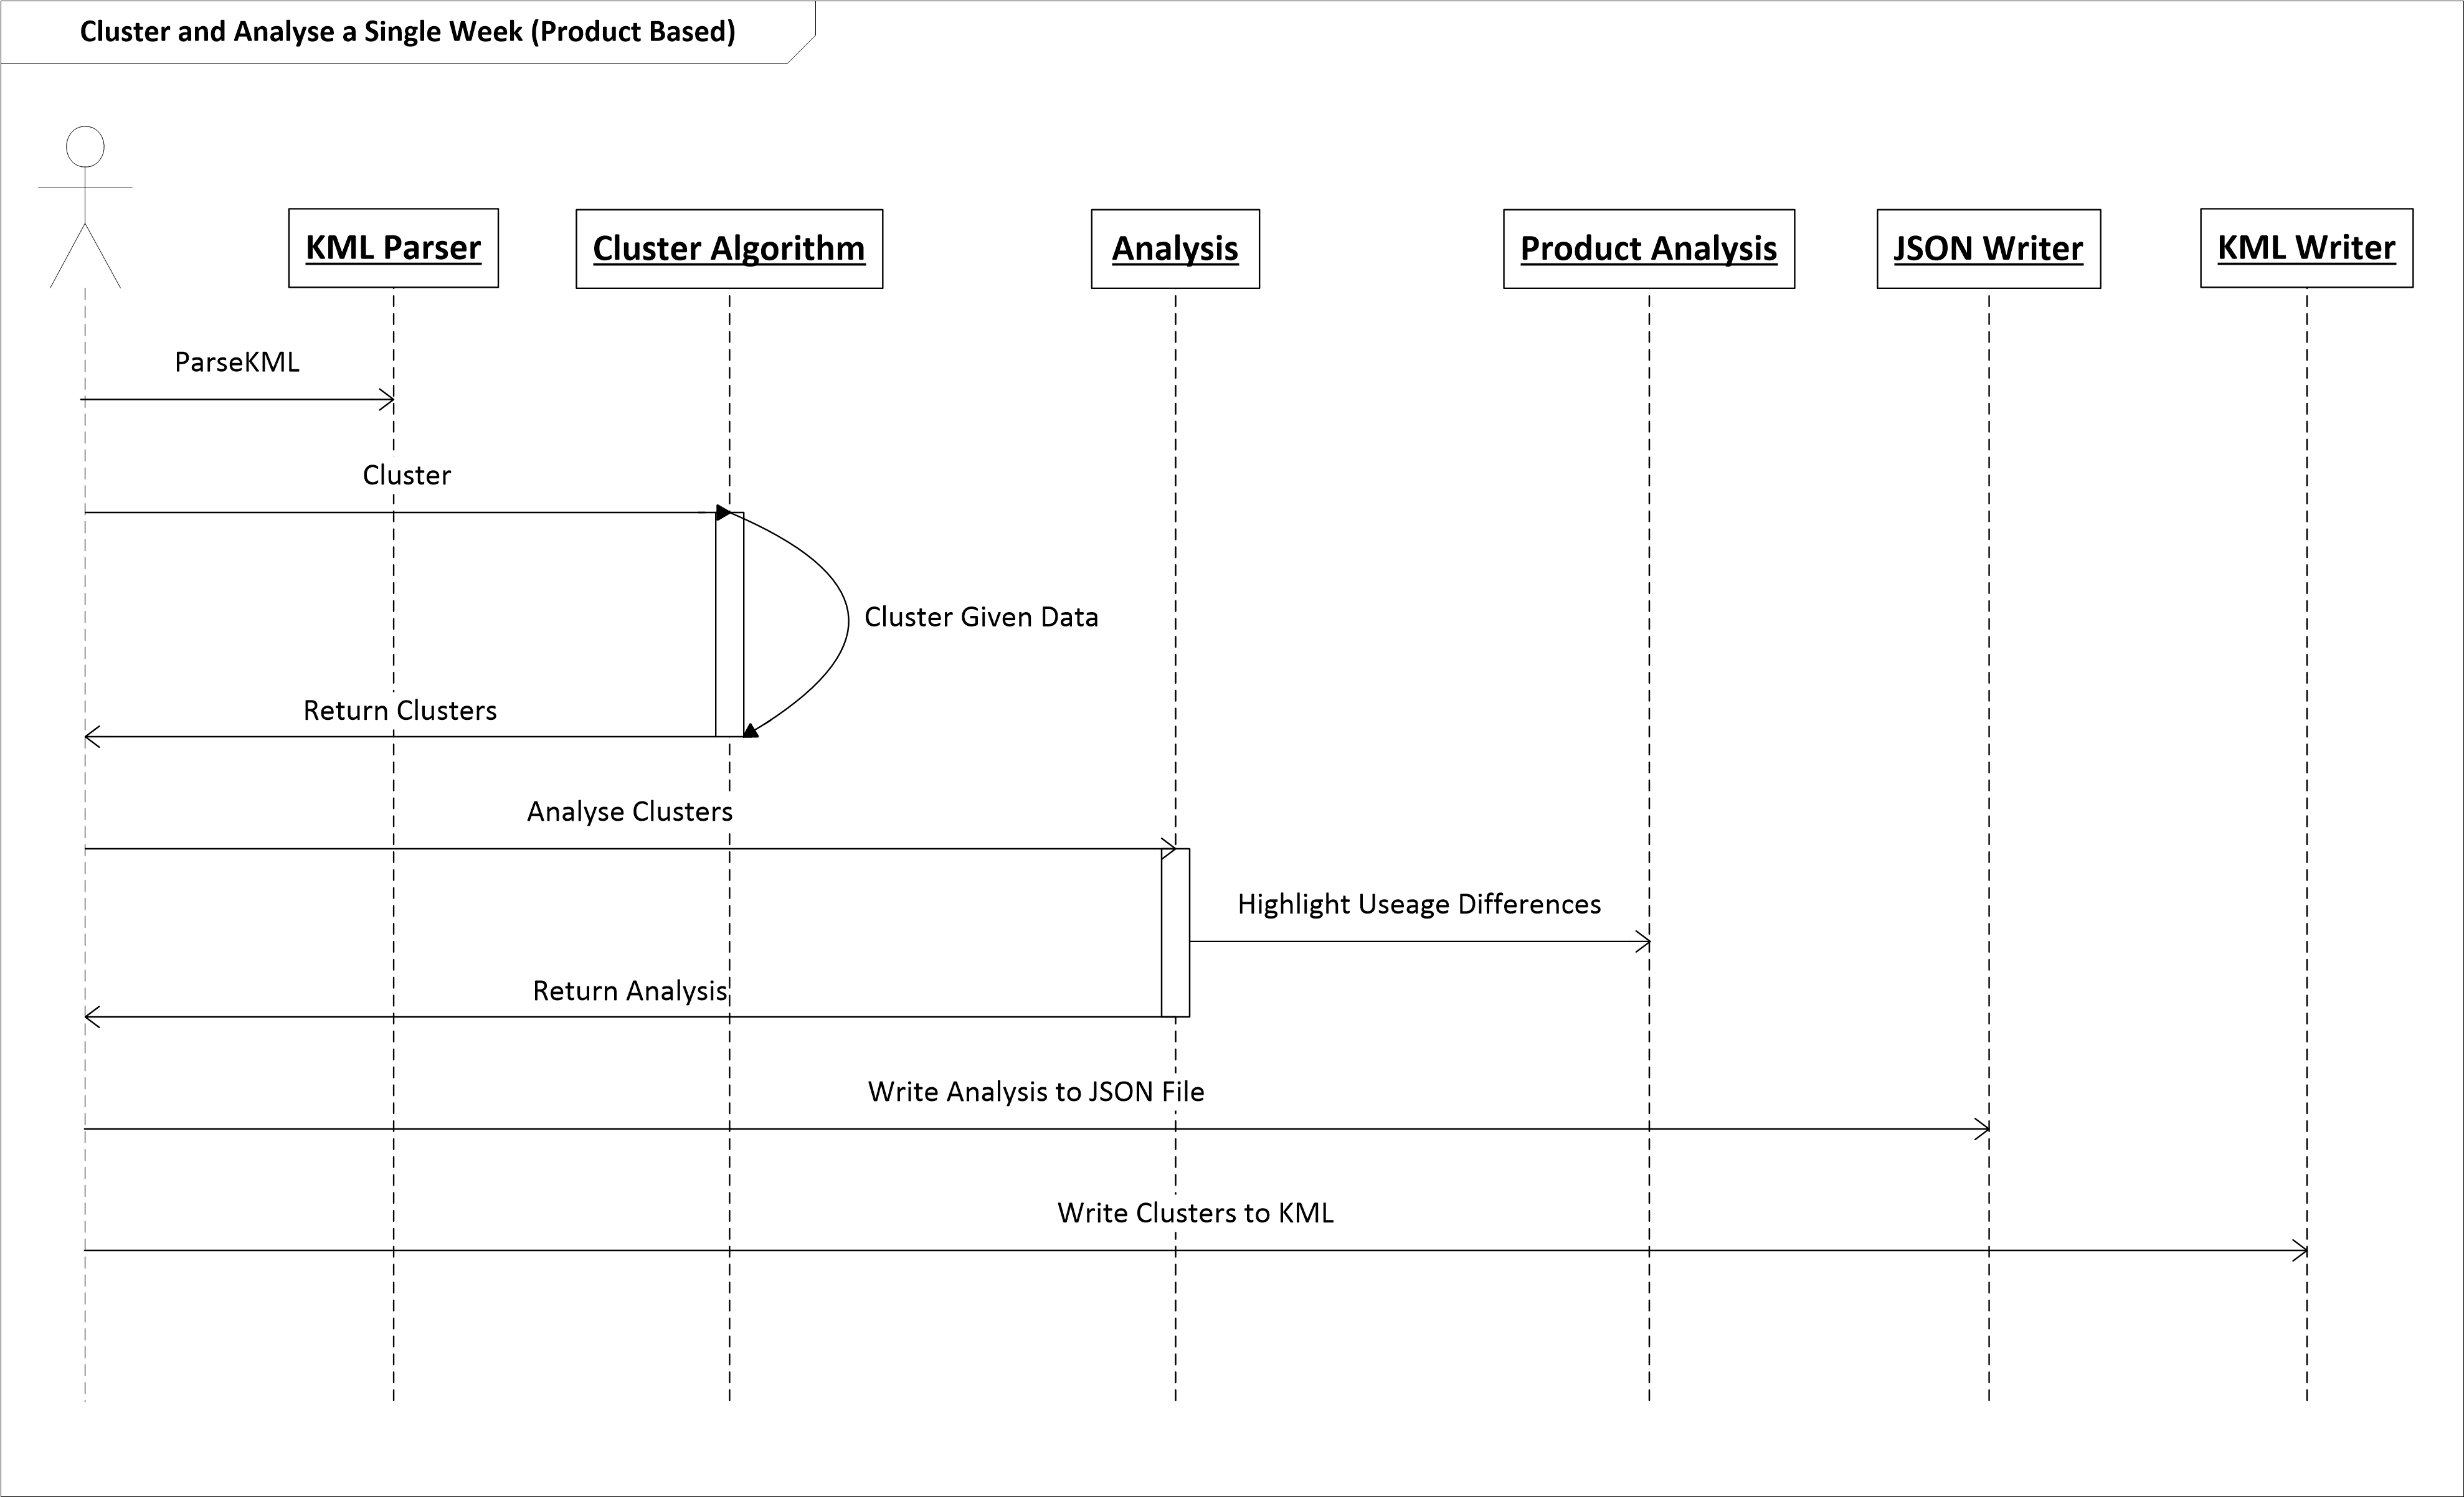
\includegraphics[scale=0.8]{chapter7/sequence_diagrams/single_week_cluster_product.png}
      \caption[Sequence diagram of a single week being clustered]
              {Sequence diagram of a single week being clustered and analysed 
              upon a product basis.}
      \label{fig:singleproduct}
  \end{figure}
\end{landscape}


\newpage
\subsection{Multi-Week Cluster and Analysis (Weekly Basis)}
Figure \ref{fig:multiweekly} highlights the sequence of events that make up 
the clustering of data and analysing the clusters upon a weekly basis.

The diagram is largely the same as the single file process, however the changes 
occur within the analysis stage of the process. The analysis event has to 
perform a number of additional analysis objectives before being able to save 
the data.

Firstly the process must highlight the differences in cluster coverings. For 
example week X may have events in clusters one to five, where as week Y may 
only have events in clusters one to three. 

Secondly, as well as presence, the process must also highlight changes to each 
cluster in real terms, such as the number increases and decreases upon a weekly 
basis. This is referred to as cluster density within the diagram.

Finally, the process must as highlight specific usage differences, such as an 
increase in 2G drops within cluster two. However this is the same as seen in 
the previous diagrams.


\afterpage{
  % Flush earlier floats (otherwise order might not be correct)
  \clearpage
  % Landscape page
  \begin{landscape}
    % Center image
    \centering 
    \begin{figure}
      \centering
        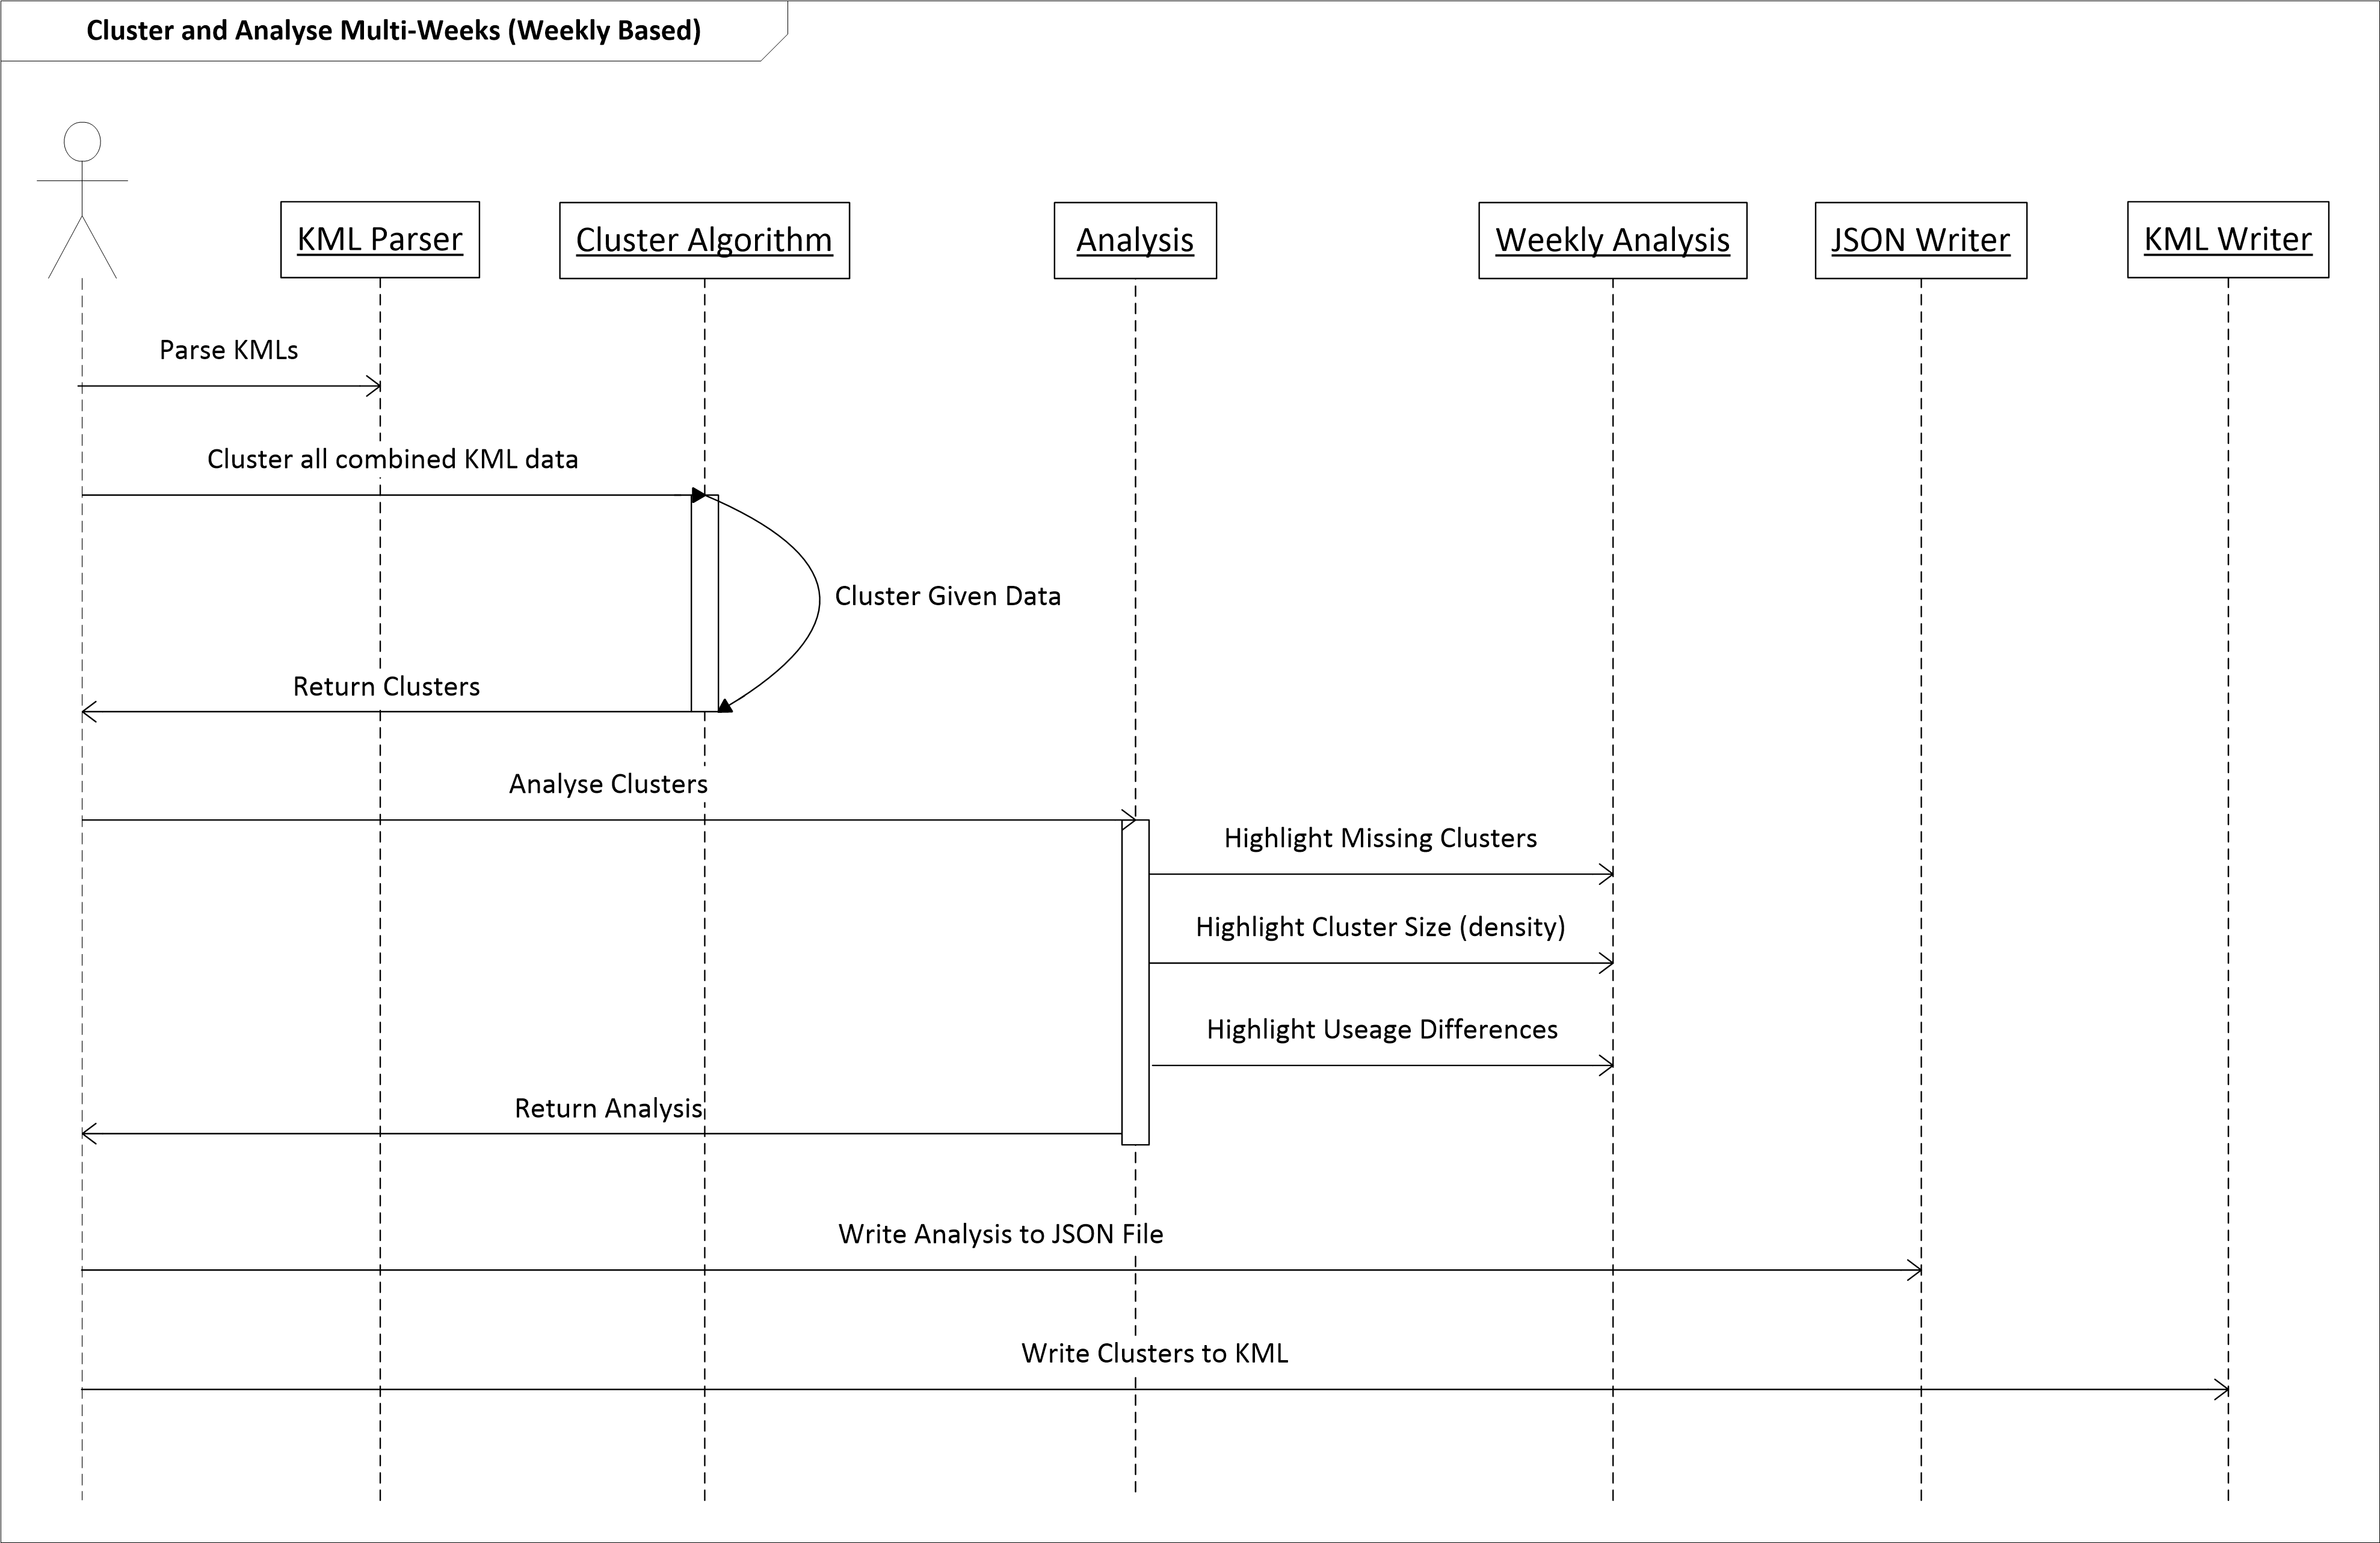
\includegraphics[scale=0.75]{chapter7/sequence_diagrams/multi_week_cluster_weekly.png}
        \caption[Sequence diagram of a multi-week being clustered]
                {Sequence diagram of a multi-week being clustered and analysed 
                upon a weekly basis.}
        \label{fig:multiweekly}
    \end{figure}
  \end{landscape}
  % Flush page
  \clearpage
}


\newpage
\subsection{Multi-Week Cluster and Analysis (Product Basis)}
Figure \ref{fig:multiproduct} highlights the sequence of events that make up 
the clustering of data and analysing the clusters upon a product basis.

The diagram is largely the same as the previous multi-week process, however the 
only change is that the pivot point is upon a product basis rather than a 
weekly-basis. For example device X may have events in clusters one to five, 
where as device Y may only have events in clusters one to three. 

As previously mentioned in all the diagrams, once the analysis has been 
completed, the results are written to a JSON file and a new output KML file.

\afterpage{
  % Flush earlier floats (otherwise order might not be correct)
  \clearpage
  % Landscape page
  \begin{landscape}
    % Center image
    \centering 
    \begin{figure}
      \centering
        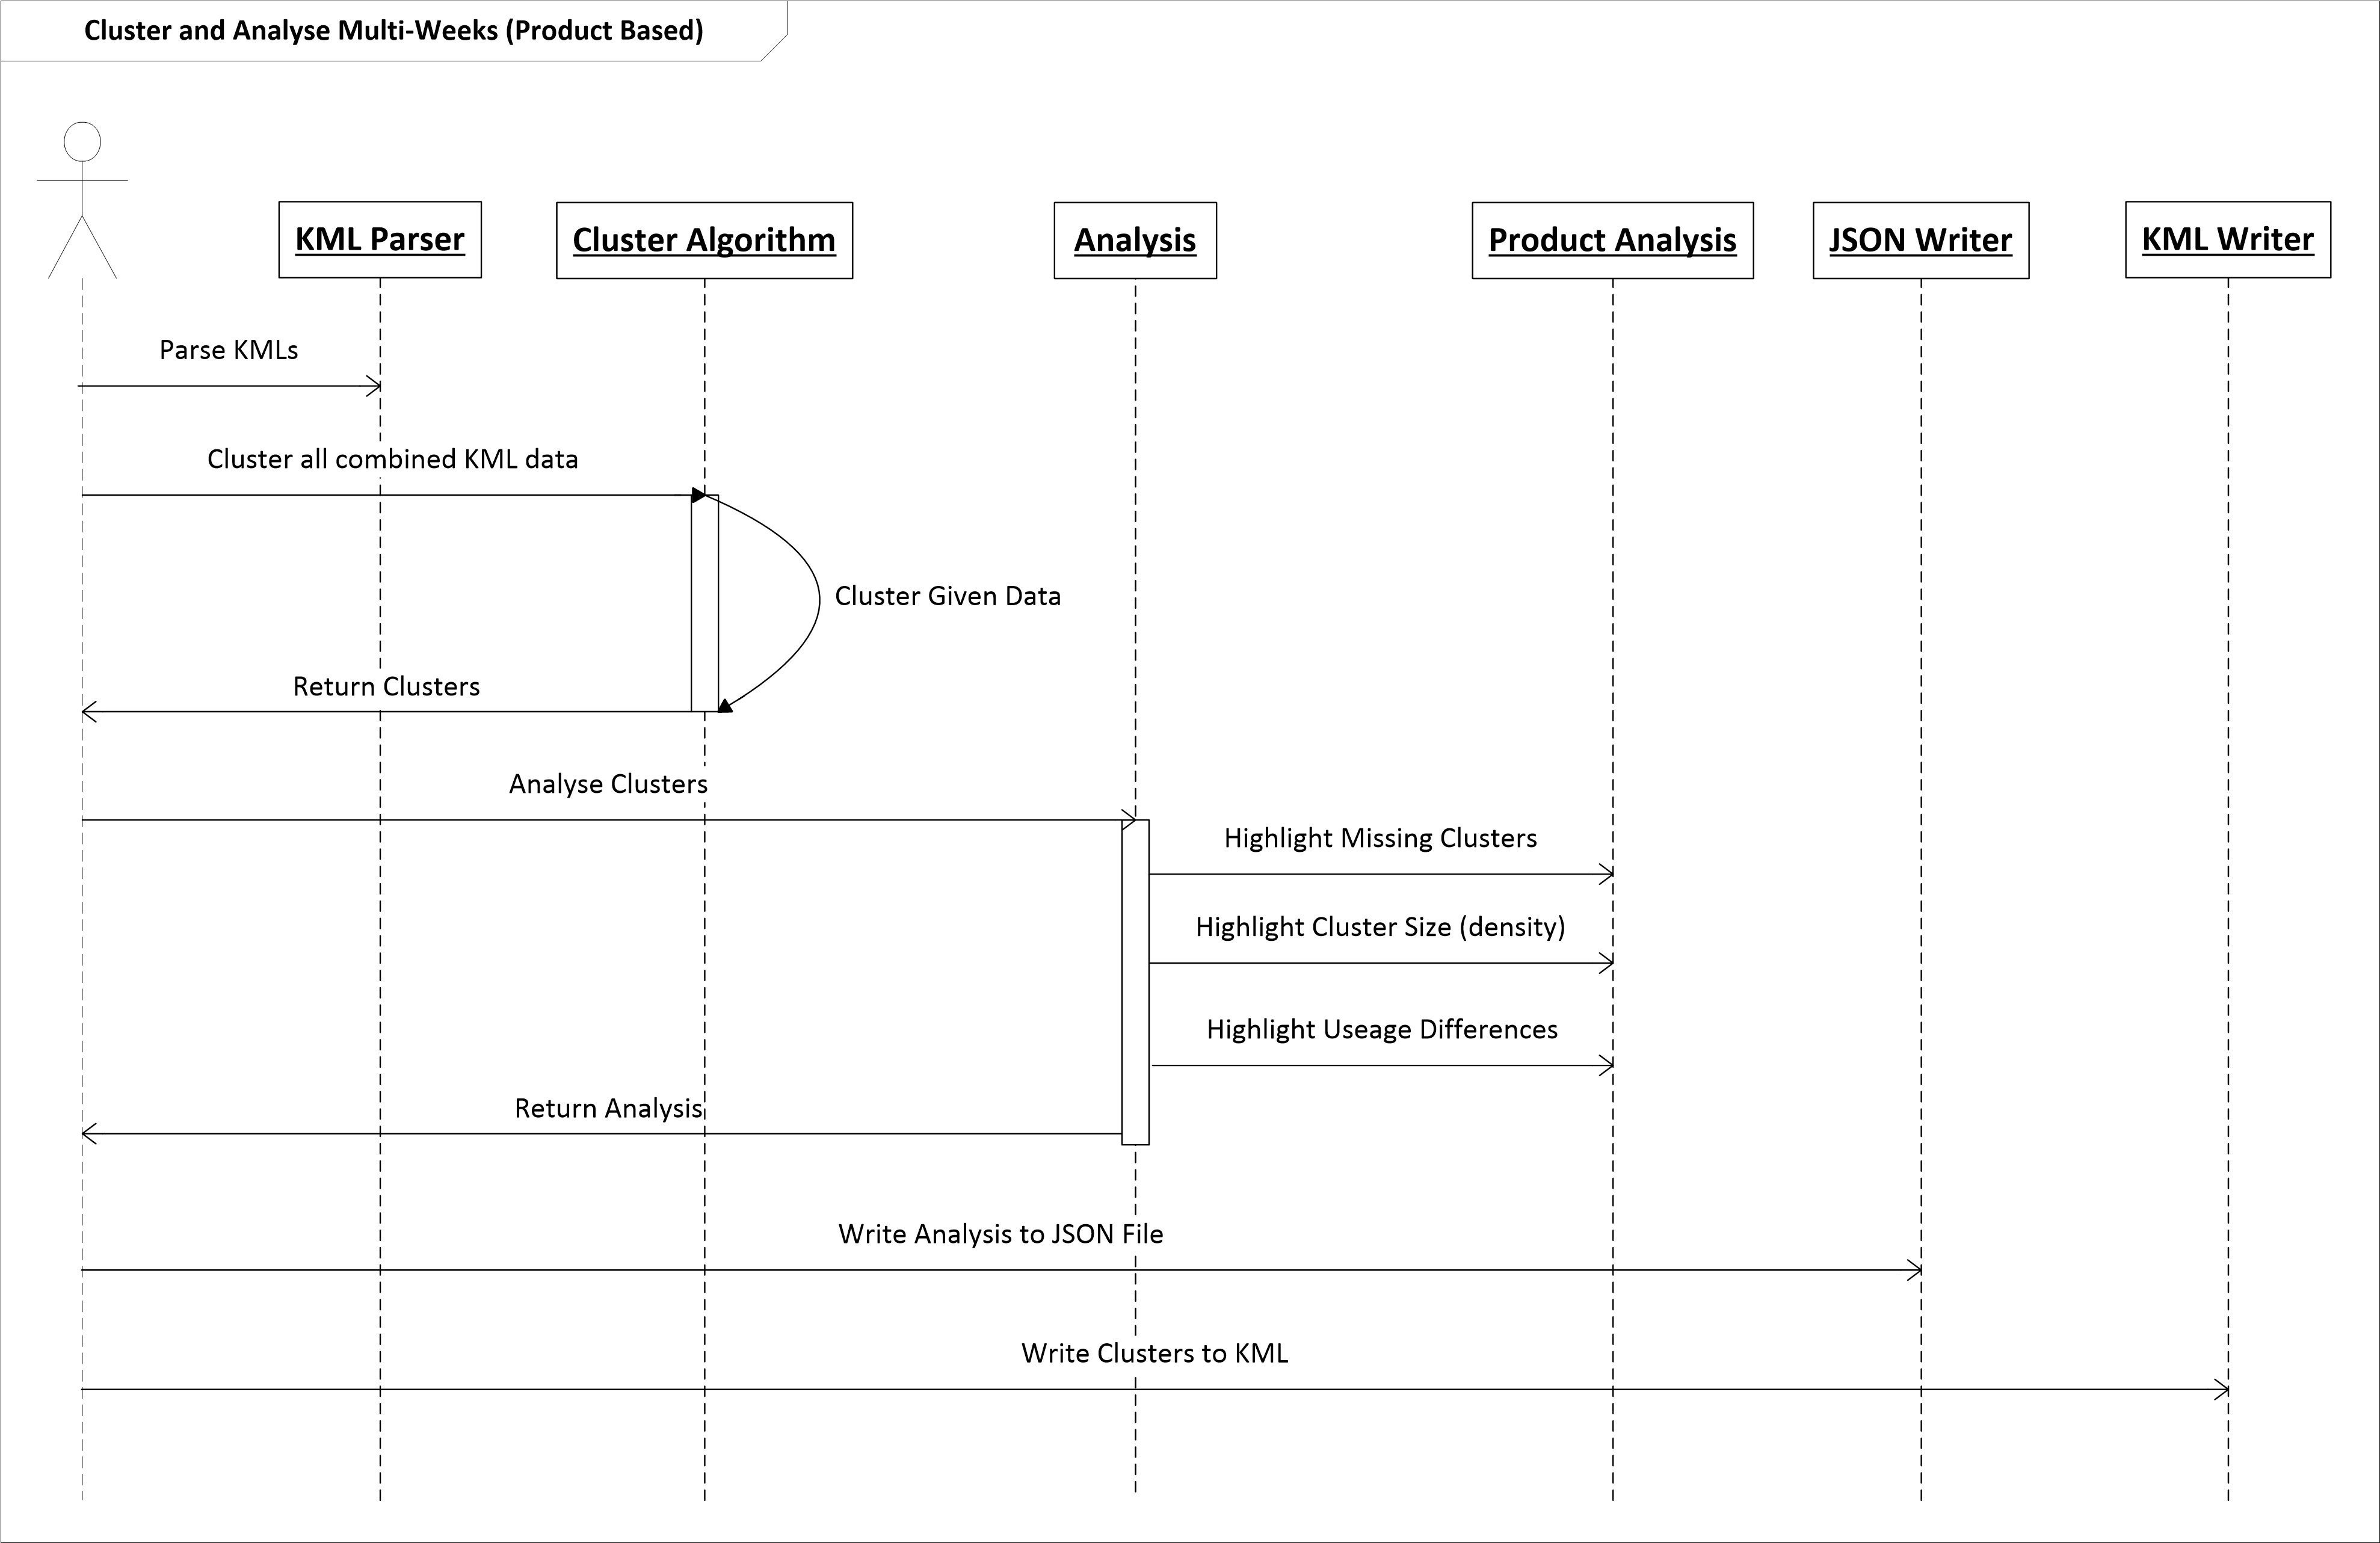
\includegraphics[scale=0.75]{chapter7/sequence_diagrams/multi_week_cluster_product.png}
        \caption[Sequence diagram of a multi-week being clustered]
                {Sequence diagram of a multi-week being clustered and analysed 
                upon a product basis.}
        \label{fig:multiproduct}
    \end{figure}
  \end{landscape}
  % Flush page
  \clearpage
}



% Class Diagrams
\newpage
\section{Class Diagrams}
A class diagram describes the structure of a system by highlighting the 
system's classes, attributes, methods, and relationships among other classes 
\citep{lunn03}.

Within this section a number of class diagrams will be presented. Each class 
diagram will represent a namespace (used to declare a scope, similar to a Java
package) in order to simplify the representation of classes. 


\subsection{Namespace Overview}
Figure \ref{fig:NSOverview} is a general overview for all the namespaces within
the system. 

Each namespace will contain specific code that is related to a certain part of 
the system's functionality. Each namespace will be compiled into a Windows 
Dynamic Link Library file (.dll). 

This will ultimately allow for re-usability for other future projects or 
extensions.

\begin{figure}[H]
  \centering
    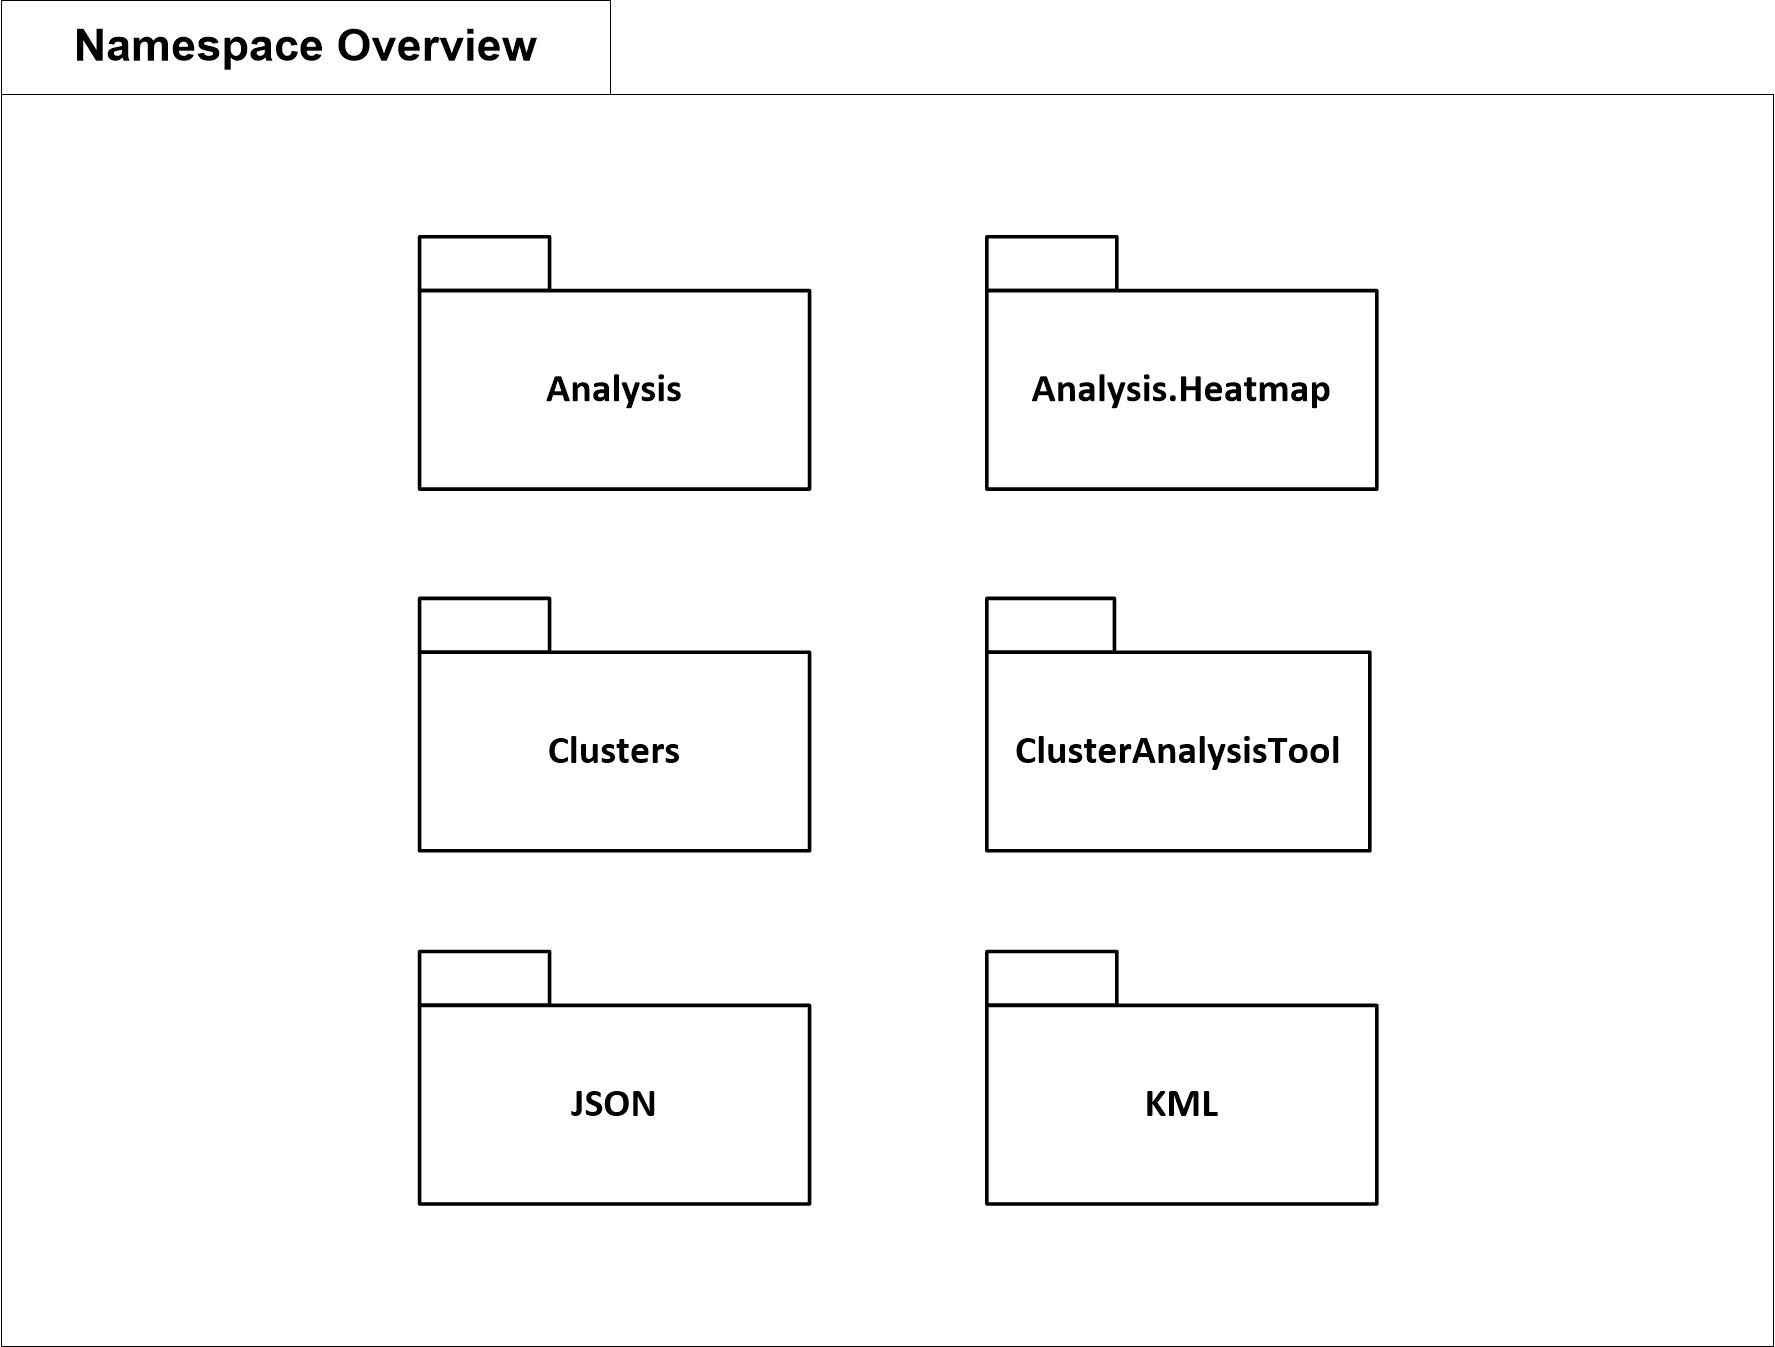
\includegraphics[scale=1.0]{chapter7/class_diagrams/namespace_overview.png}
    \caption[Overview of the entire Cluster Analysis Solution]
            {Overview of the entire Cluster Analysis Solution.}
    \label{fig:NSOverview}
\end{figure}



\subsection{Analysis}
Figure \ref{fig:NSAnalysis} shows the Analysis namespace, which provides the 
system with all the analysis classes, business logic and template output files. 

The Event Analysis class is an abstract class (indicated by the italic name), 
which is able to to provide generic functionality to analyse Drop and Fail 
events. Any additional Drop and Fail analysis will placed into these classes.
It is these classes that provide analysis upon one type of event within one
cluster.

The Cluster Analysis object is the main entry point for analysing a given 
cluster with a set of clusters. This class provides functionality to directly 
make use of the methods found within the DropAnalysis and FailAnalysis classes.

The Analysis class is another abstract class than provides analysis for a group 
of clusters. The Product Analysis and Week Analysis classes extend the Analysis
class to provide four specific forms of analysis. 

By utilising both the DropAnalysis and FailAnalysis classes, the Product 
Analysis and Week Analysis classes are able to analyse an entire product or 
week respectfully.

The AnalysisResults and AnalysisResultsCollection classes are alias classes for
complex dictionary objects. Both of these classes will store the results 
generated by the analysis classes as key/value pair lists. 

The JSON results class stores a number of AnalysisResultsCollection objects for
easy converting to a JSON format.

The MultiAnalysis class provides a base class for different forms of analysis 
to easily happen. The MutliWeekAnalysis class extends the MultiAnalysis class, 
which allows for easy access to analyse all the given weeks (or an individual 
week). 

This class possess functionality to output all analysis as a JSON string or as 
a JSON file.

\begin{figure}[H]
  \centering
    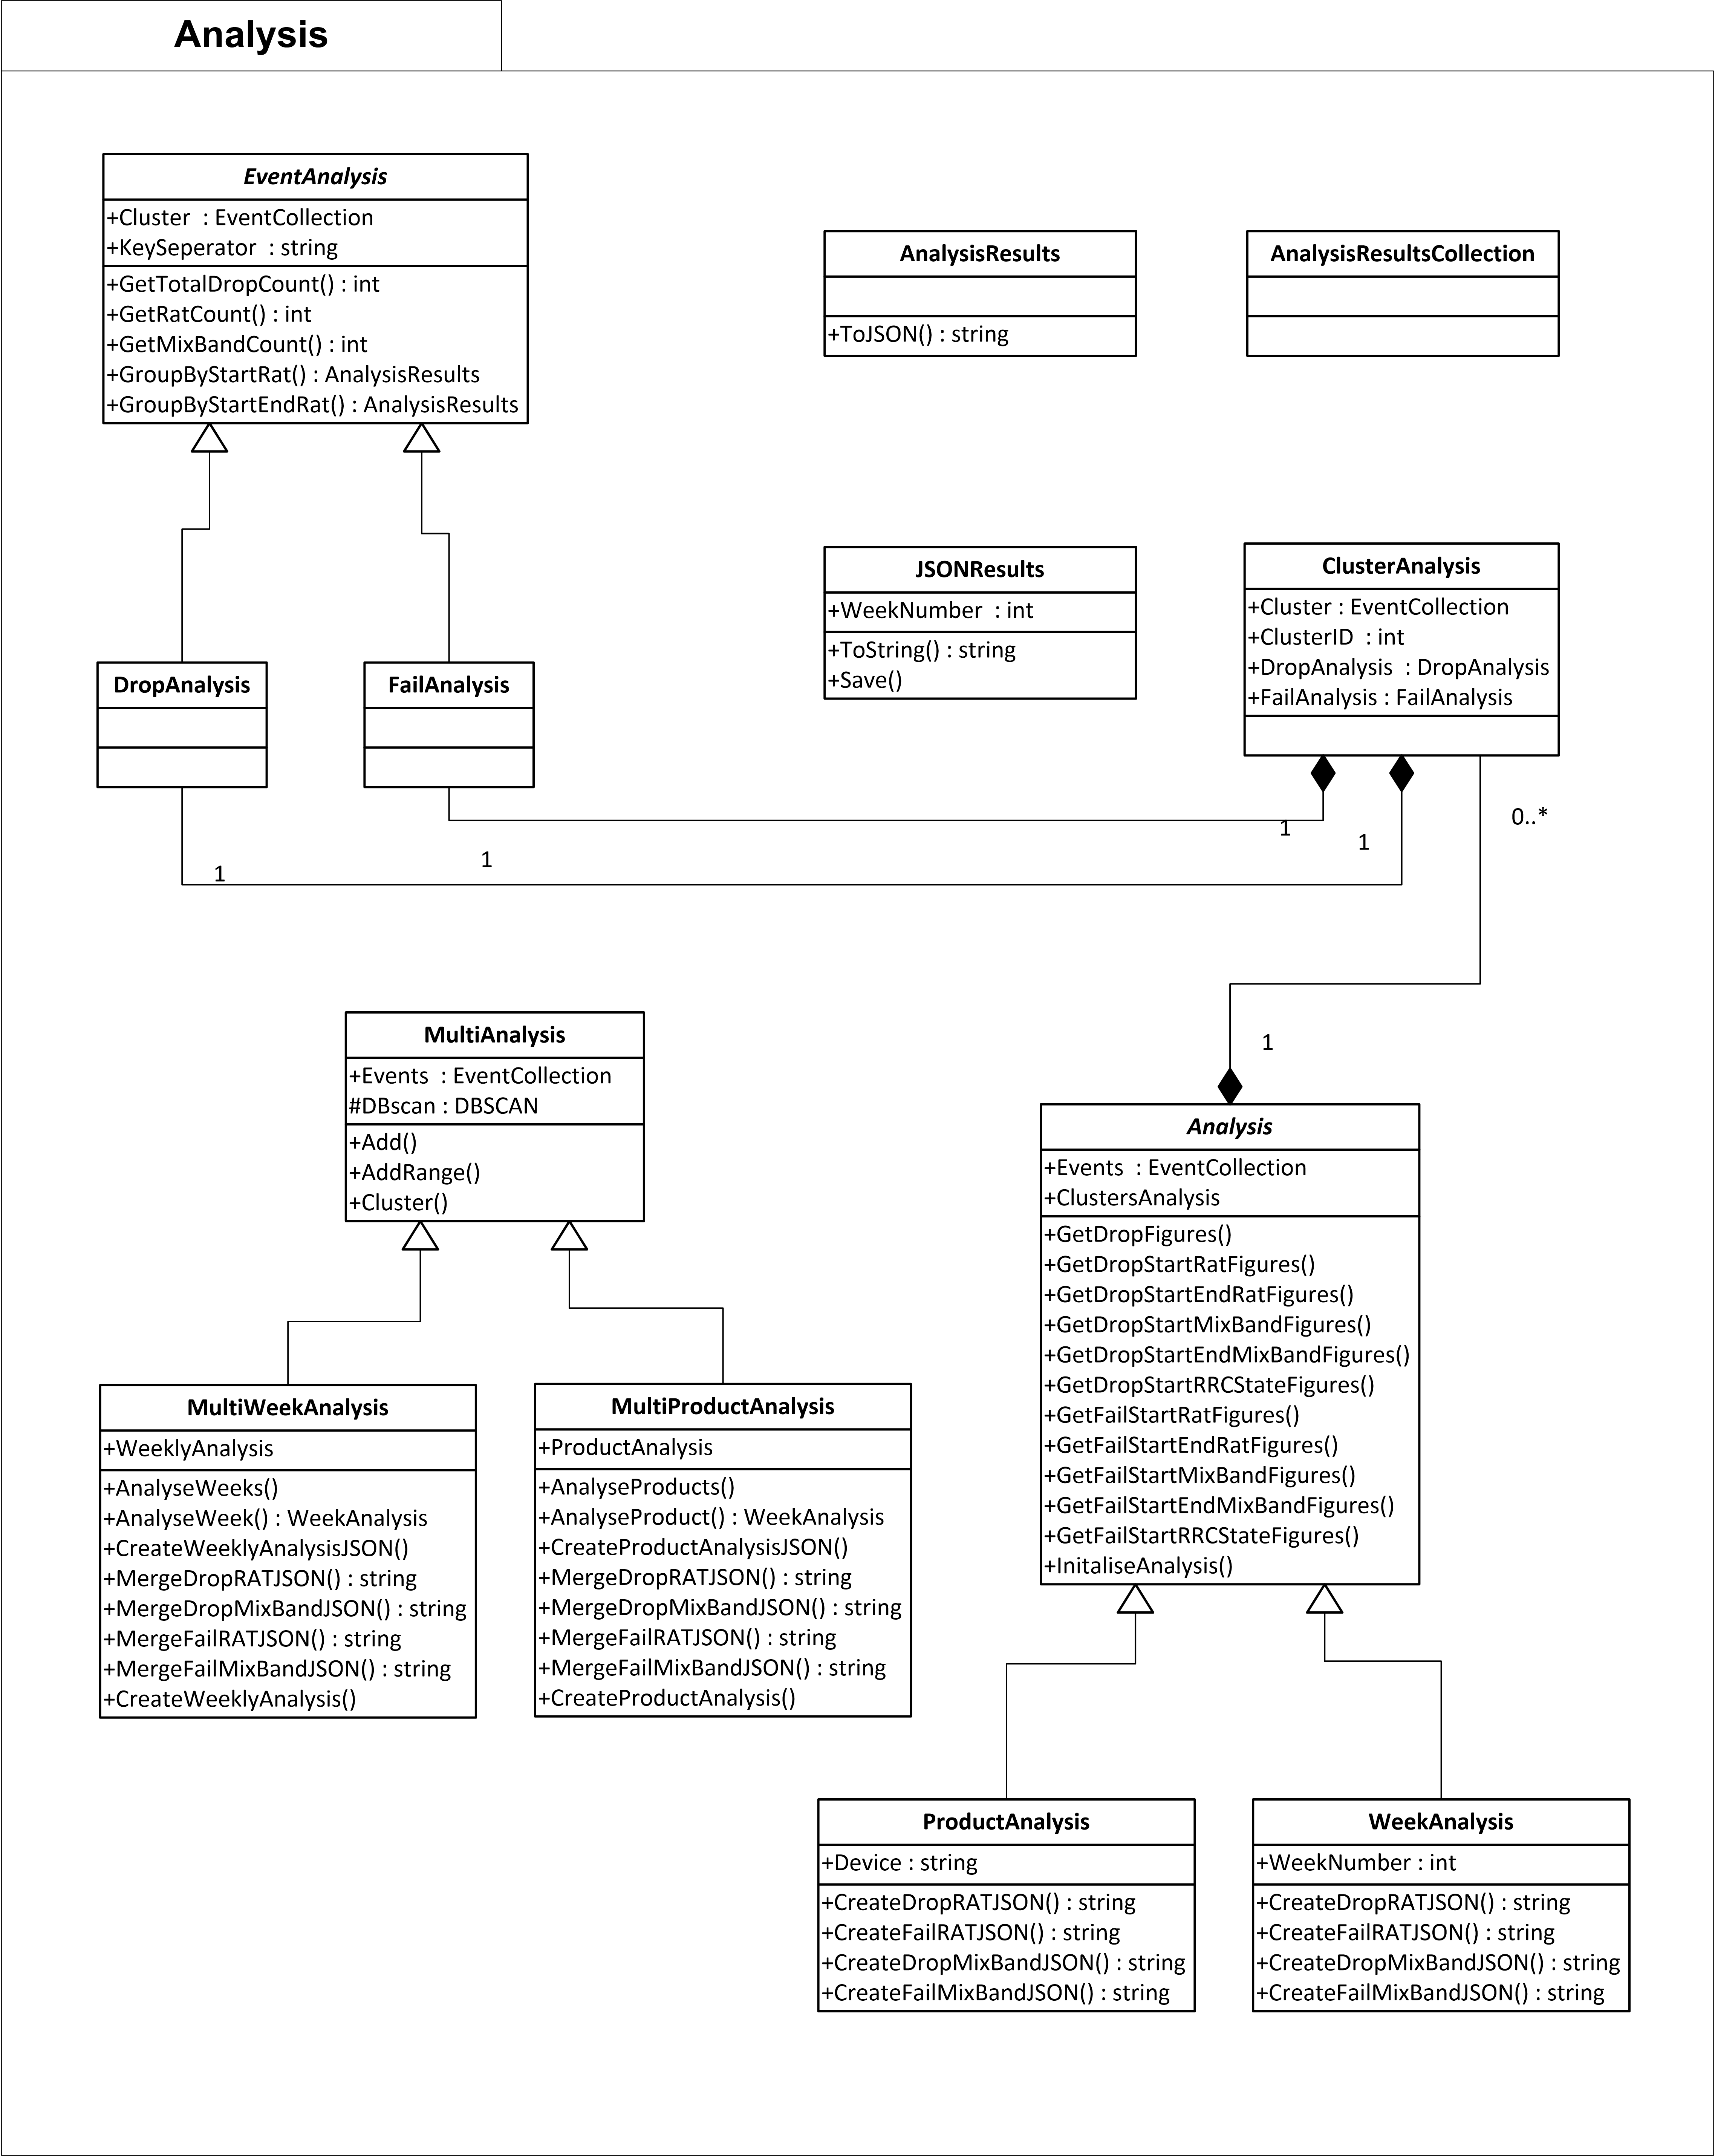
\includegraphics[scale=0.8]{chapter7/class_diagrams/analysis_namespace.png}
    \caption[Analysis namespace class diagram]
            {Analysis namespace class diagram.}
    \label{fig:NSAnalysis}
\end{figure}



\subsection{Analysis.Heatmap}
Figure \ref{fig:NSHeatmap} shows the Analysis.Heatmap namespace, which is a 
sub namespace of the main analysis class. This namespace provides functionality 
to allow for heatmaps to be created. to highlight high object intensity upon a 
map.

The Heatmap class is the main entry point to create a heatmap. The class will 
convert an EventCollection a collection of HeatPoints. The conversion involves 
mapping a GPS coordinate to a screen coordinate, and assigning it an intensity 
weighting. 

The ColorScheme class will provide a set number of colour schemes, to allow for 
the user to change the colour scheme of the heatmap.

\begin{figure}[H]
  \centering
    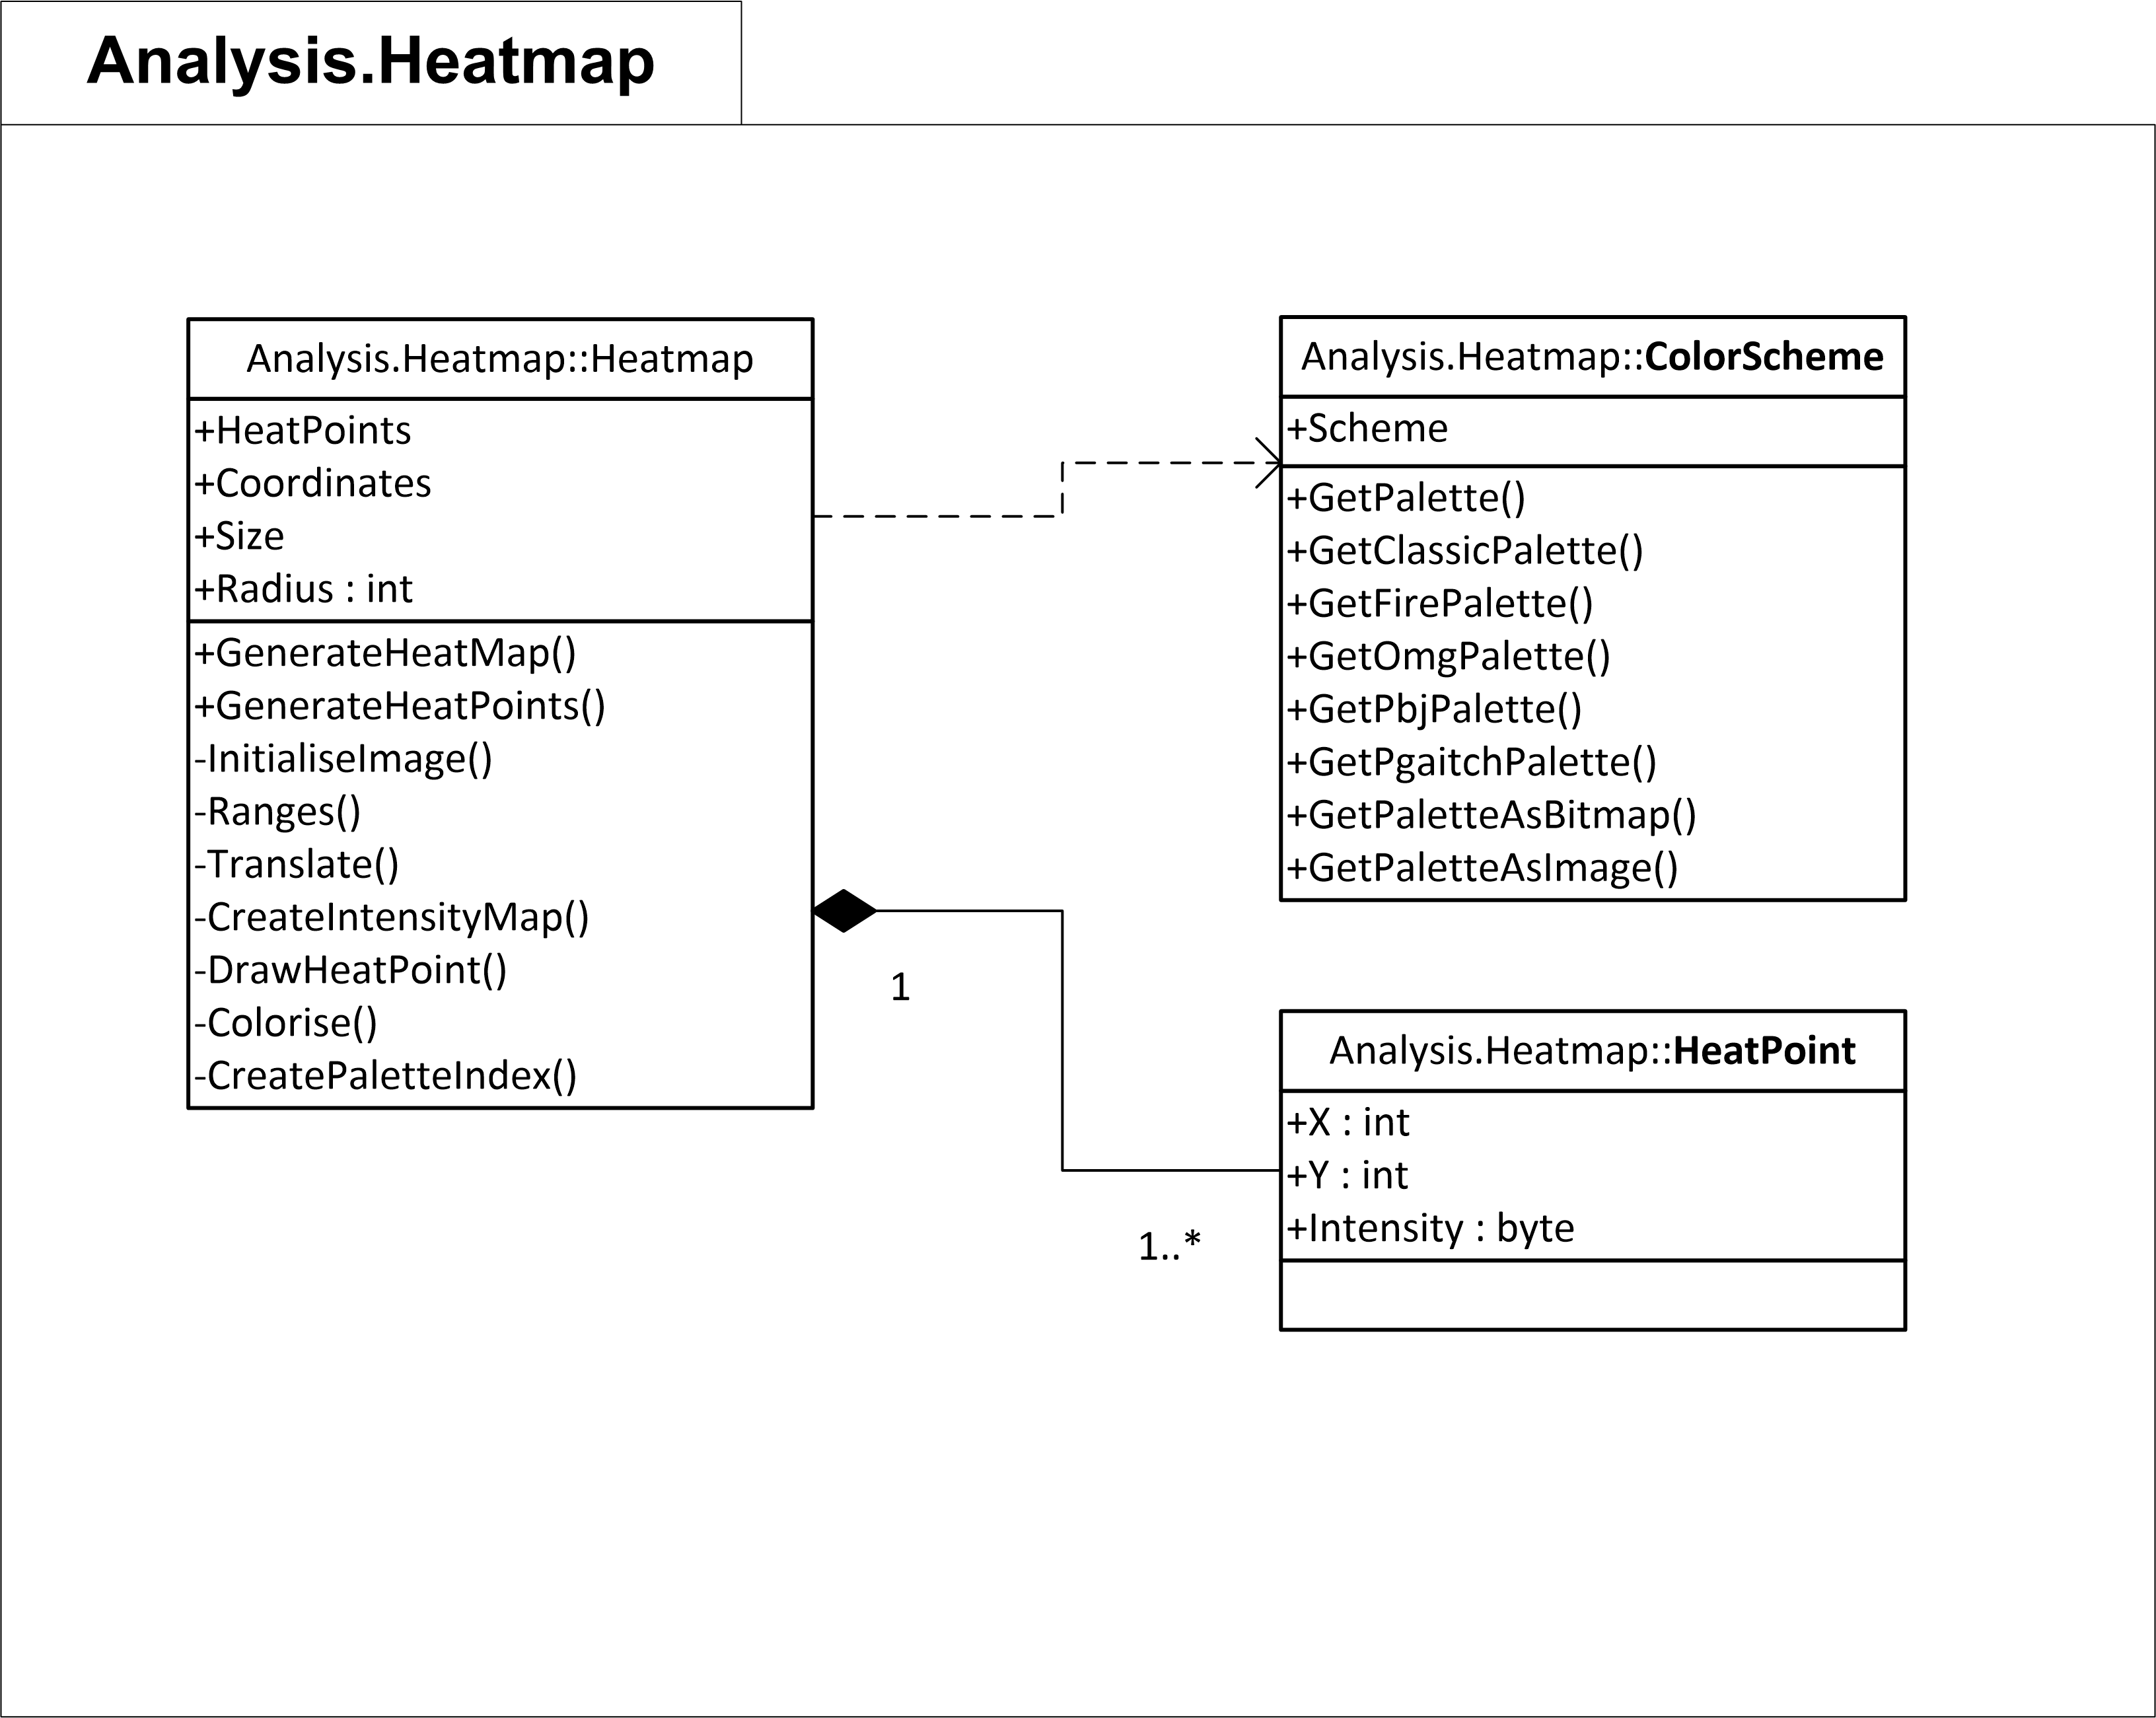
\includegraphics[scale=0.9]{chapter7/class_diagrams/analysis_heatmap_namespace.png}
    \caption[Analysis.Heapmap namespace class diagram]
            {Analysis.Heatmap namespace class diagram.}
    \label{fig:NSHeatmap}
\end{figure}



\subsection{Clusters}
Figure \ref{fig:NSClusters} shows the Clusters namespace, which provides the 
system with the ability to cluster events. Additional fundamental classes such 
as Events, Coordinates and their respected collections can also be found within
this namespace.

At the simplest level, the Coordinate class represents a GPS Coordinate, along 
with some additional values that are used by the clustering algorithms. The 
Centroid class extends the coordinate class to add the radius field, which holds
the size of the radius. 

The Event class is an abstract class that models a given event. Additional 
details such as device, pin, timestamp etc are stored along with the Coordinate 
of the event. The event class can not be directly instantiated, and thus there 
are a number of classes for each type of event, Fail, Success and Drop.

The EventCollection and CoordinateCollection both extend the List, to allow for 
any number of events and coordinates to be stored in a collection. Events and 
coordinates can not be mixed up in the same collections. Each collection 
provides the same methods, that allow the elements to be manipulated easily.

The RadialCircle class allows a radius to be draw around a given point, with a 
given radius. The SphericalCoordinate provides additional support for this 
feature. The Distance class is a static class that calculates the distance 
between two given coordinates based upon a number of formulas. Each formula has 
a different accuracy level.

The DBSCAN and K-Means classes both provide an implementation to the DBSCAN and
K-Means algorithms respectfully. Each take either an EventCollection and return 
a List of EventCollections. Each element within the list represents a cluster. 
The DBSCAN class has an additional field which stores events and coordinates 
that are deemed to be ``noisy''.

\begin{figure}[H]
  \centering
    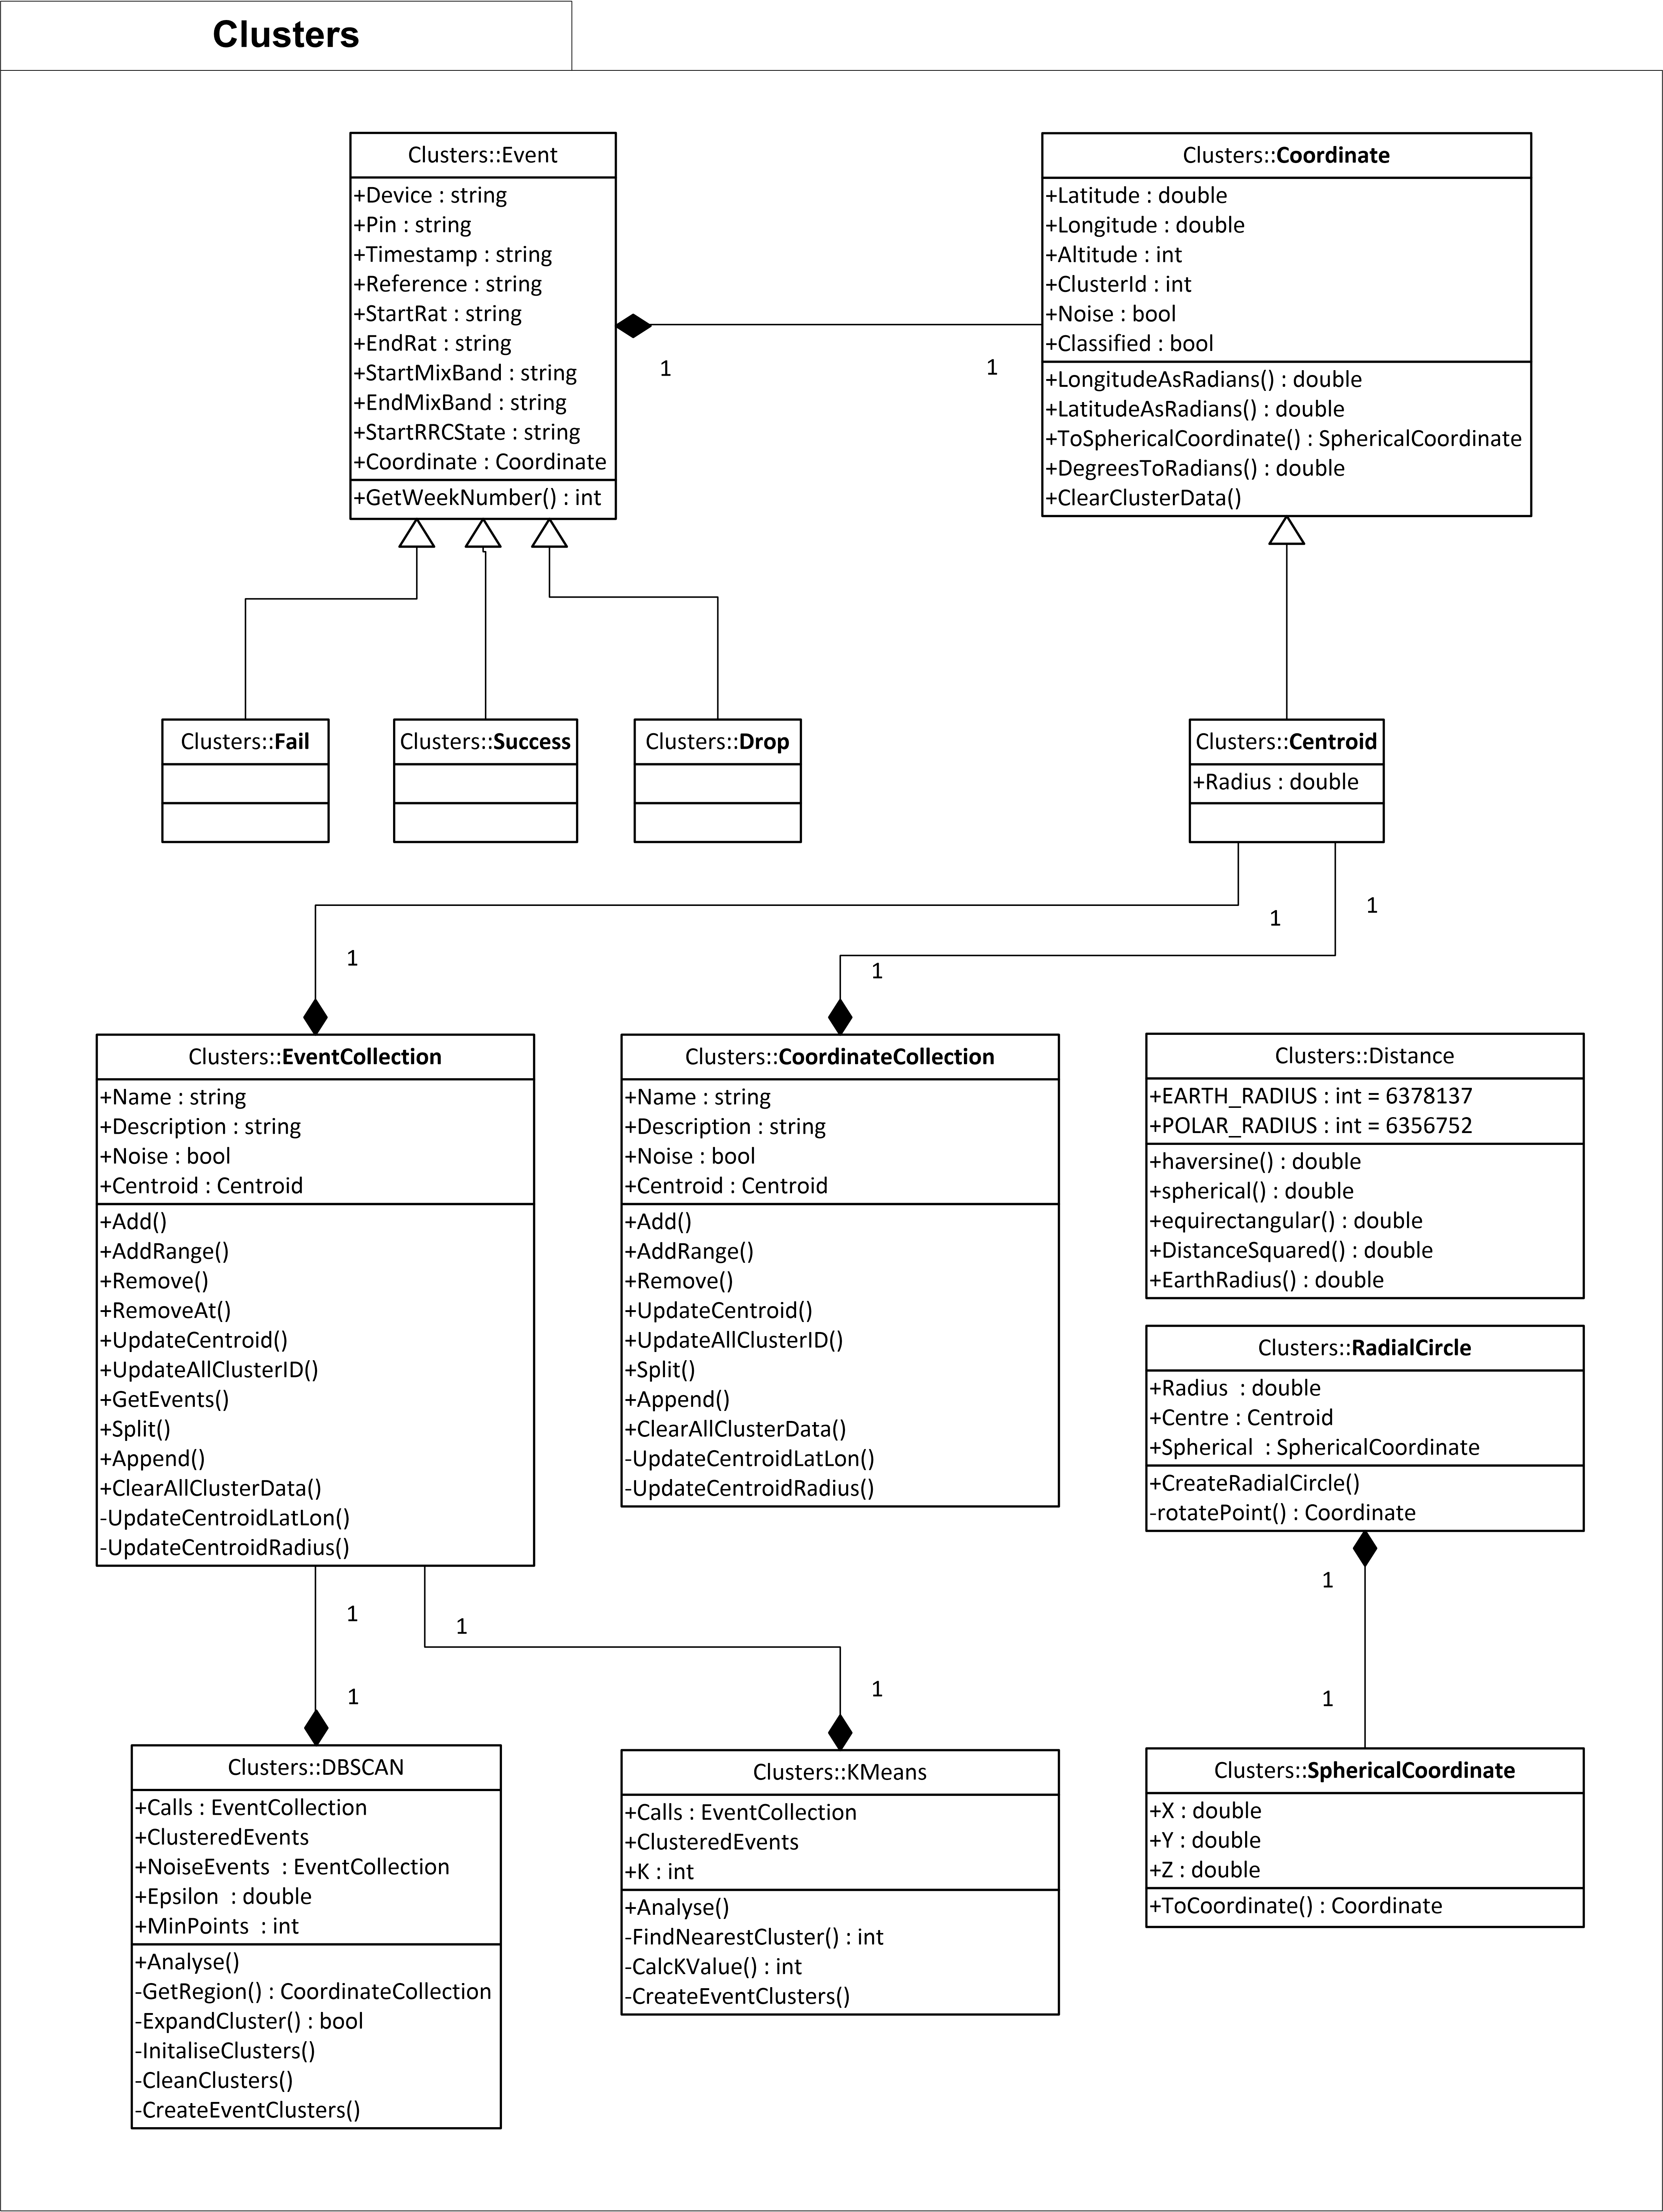
\includegraphics[scale=0.8]{chapter7/class_diagrams/clusters_namespace.png}
    \caption[Clusters namespace class diagram]
            {Clusters namespace class diagram.}
    \label{fig:NSClusters}
\end{figure}


\subsection{ClusterAnalysisTool}
Figure \ref{fig:NSClusterAnalysisTool} highlights the namespace that provides 
the main entry point to the tool. When complied this namespace will form an 
executable file (.exe) that allows the user to run the program via the command 
line. This is expressed in the Program file.

The Arguments class is a utility class for the Program file, which allows for 
easy parsing of (optionally) passed flags.

\begin{figure}[H]
  \centering
    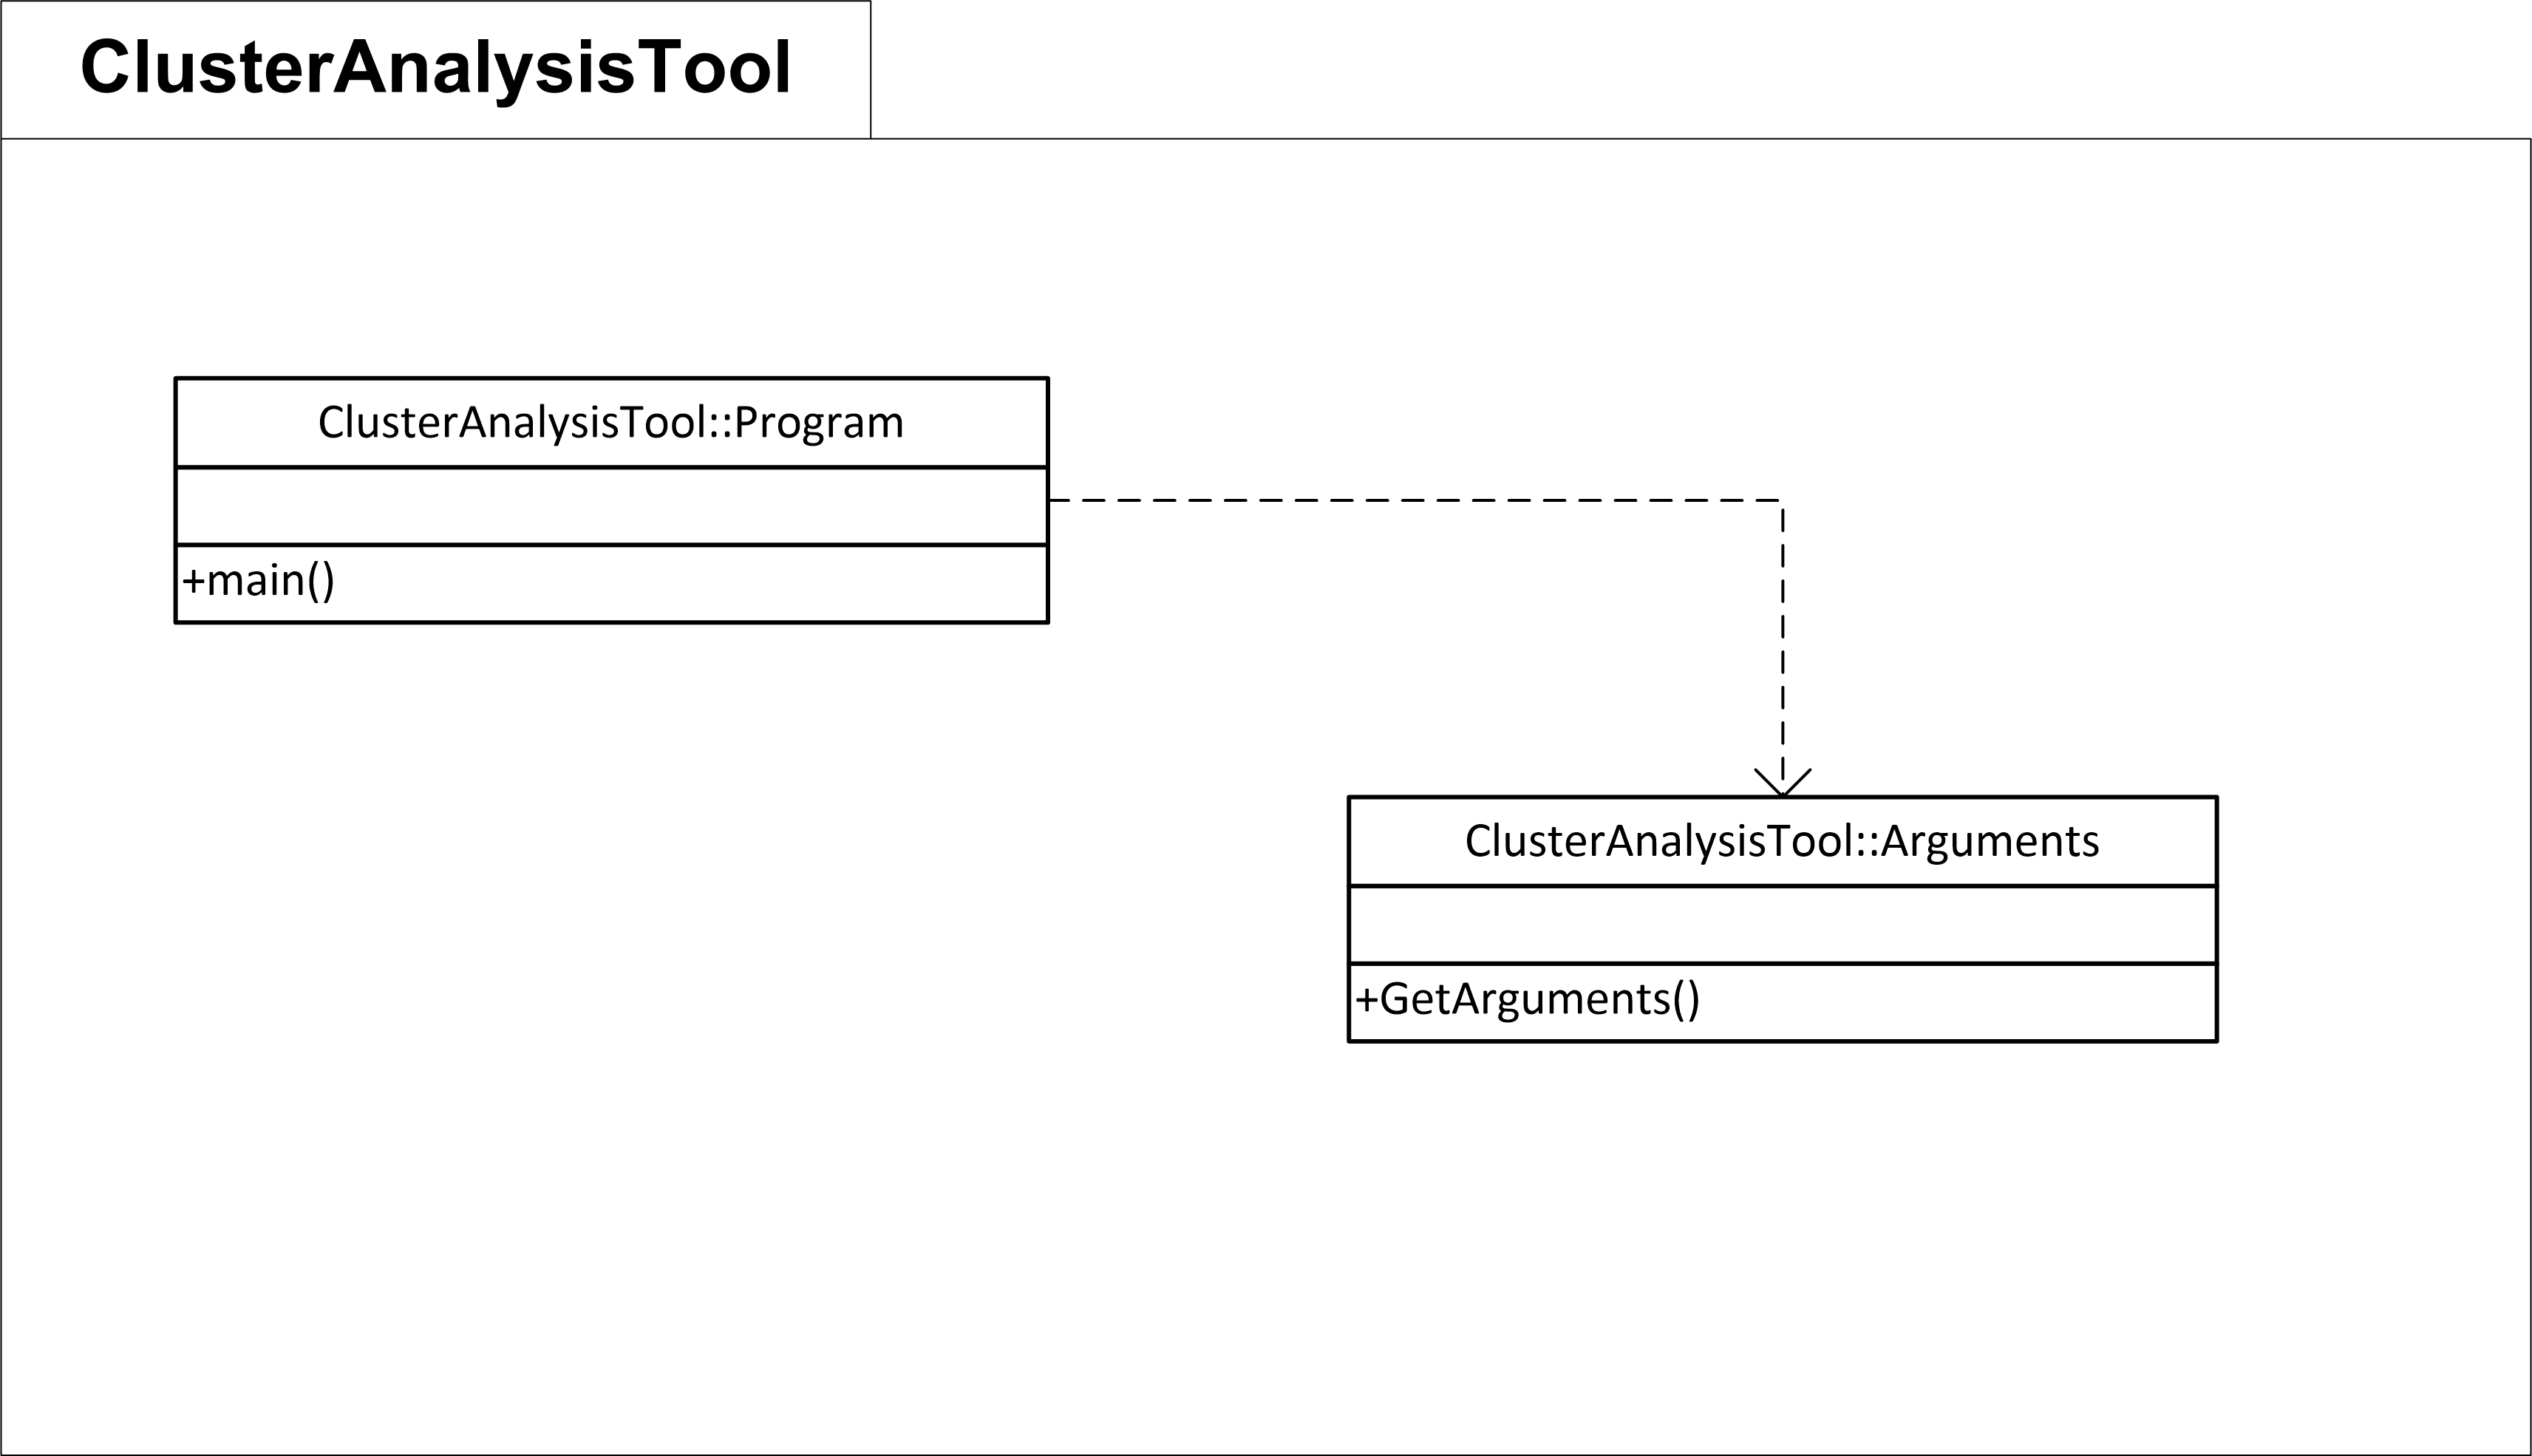
\includegraphics[scale=0.9]{chapter7/class_diagrams/clusteranalysistool_namespace.png}
    \caption[ClusterAnalysisTool namespace class diagram]
            {ClusterAnalysisTool namespace class diagram.}
    \label{fig:NSClusterAnalysisTool}
\end{figure}



\subsection{JSON}
Figure \ref{fig:NSJSON} highlights the namespace that handles creating well 
formed, sound JSON strings. This namespace, can be thought of a utility 
namespace.

This only class within this namespace, JSON, is a static class, and requires no 
instantiation. It creates a number of fundamental JSON strings, as well as 
being able to expand minified JSON code (referred to as prettify).

\begin{figure}[H]
  \centering
    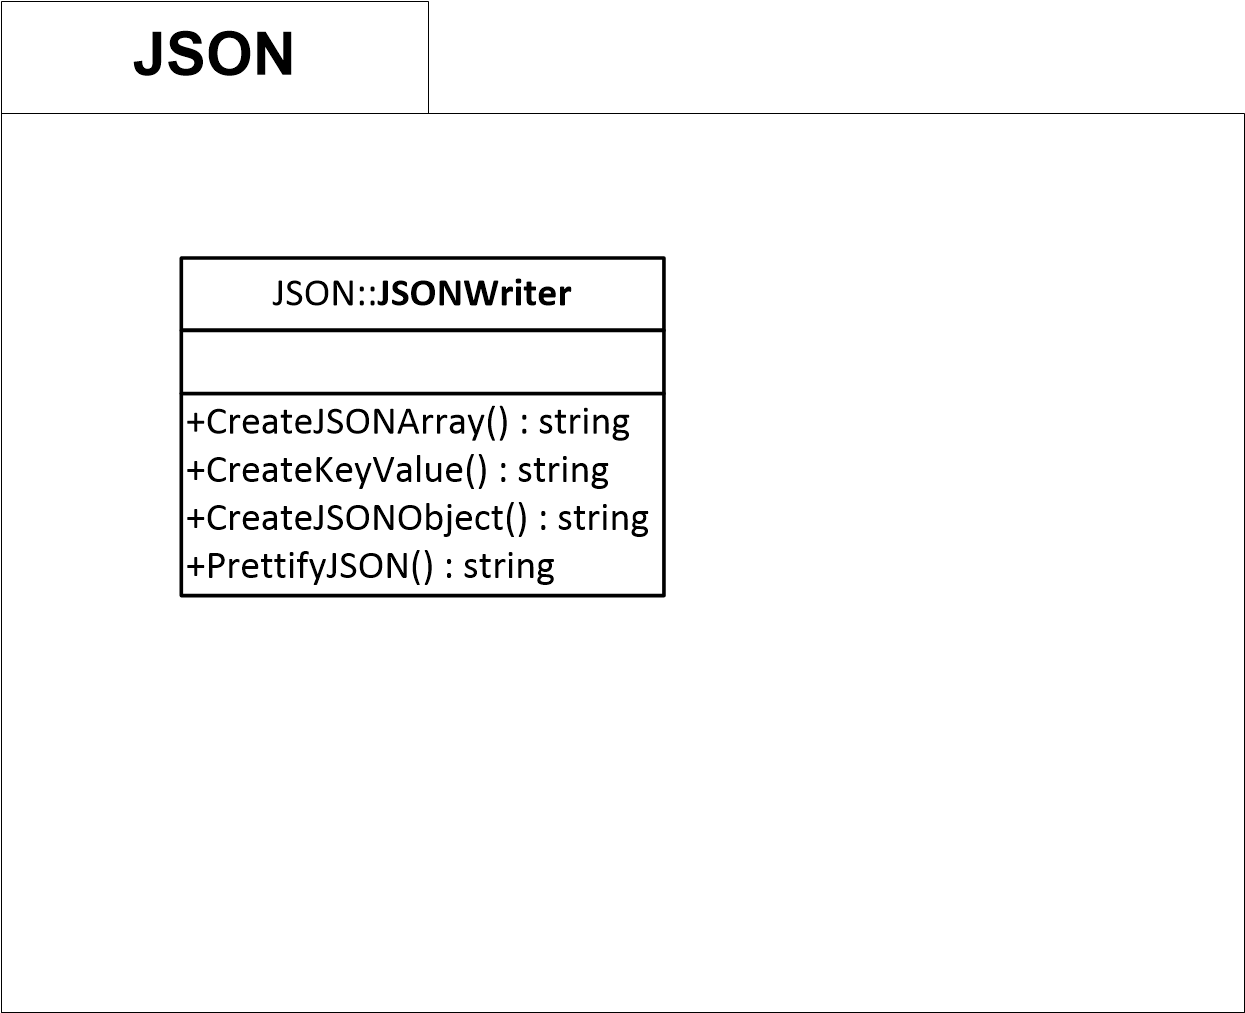
\includegraphics[scale=0.9]{chapter7/class_diagrams/json_namespace.png}
    \caption[JSON namespace class diagram]
            {JSON namespace class diagram.}
    \label{fig:NSJSON}
\end{figure}



\subsection{KML}
Figure \ref{fig:NSKML} highlights the namespace that handles the reading and 
writing of KML files. This namespace, like the JSON namespace, can be thought 
of a utility namespace.

The KML Writer class will create a well formed KML file, that can be opened 
from within Google Earth. 

The KML Reader class will read a KML file into an EventCollection object, which 
can be used in various other namespaces.

\begin{figure}[H]
  \centering
    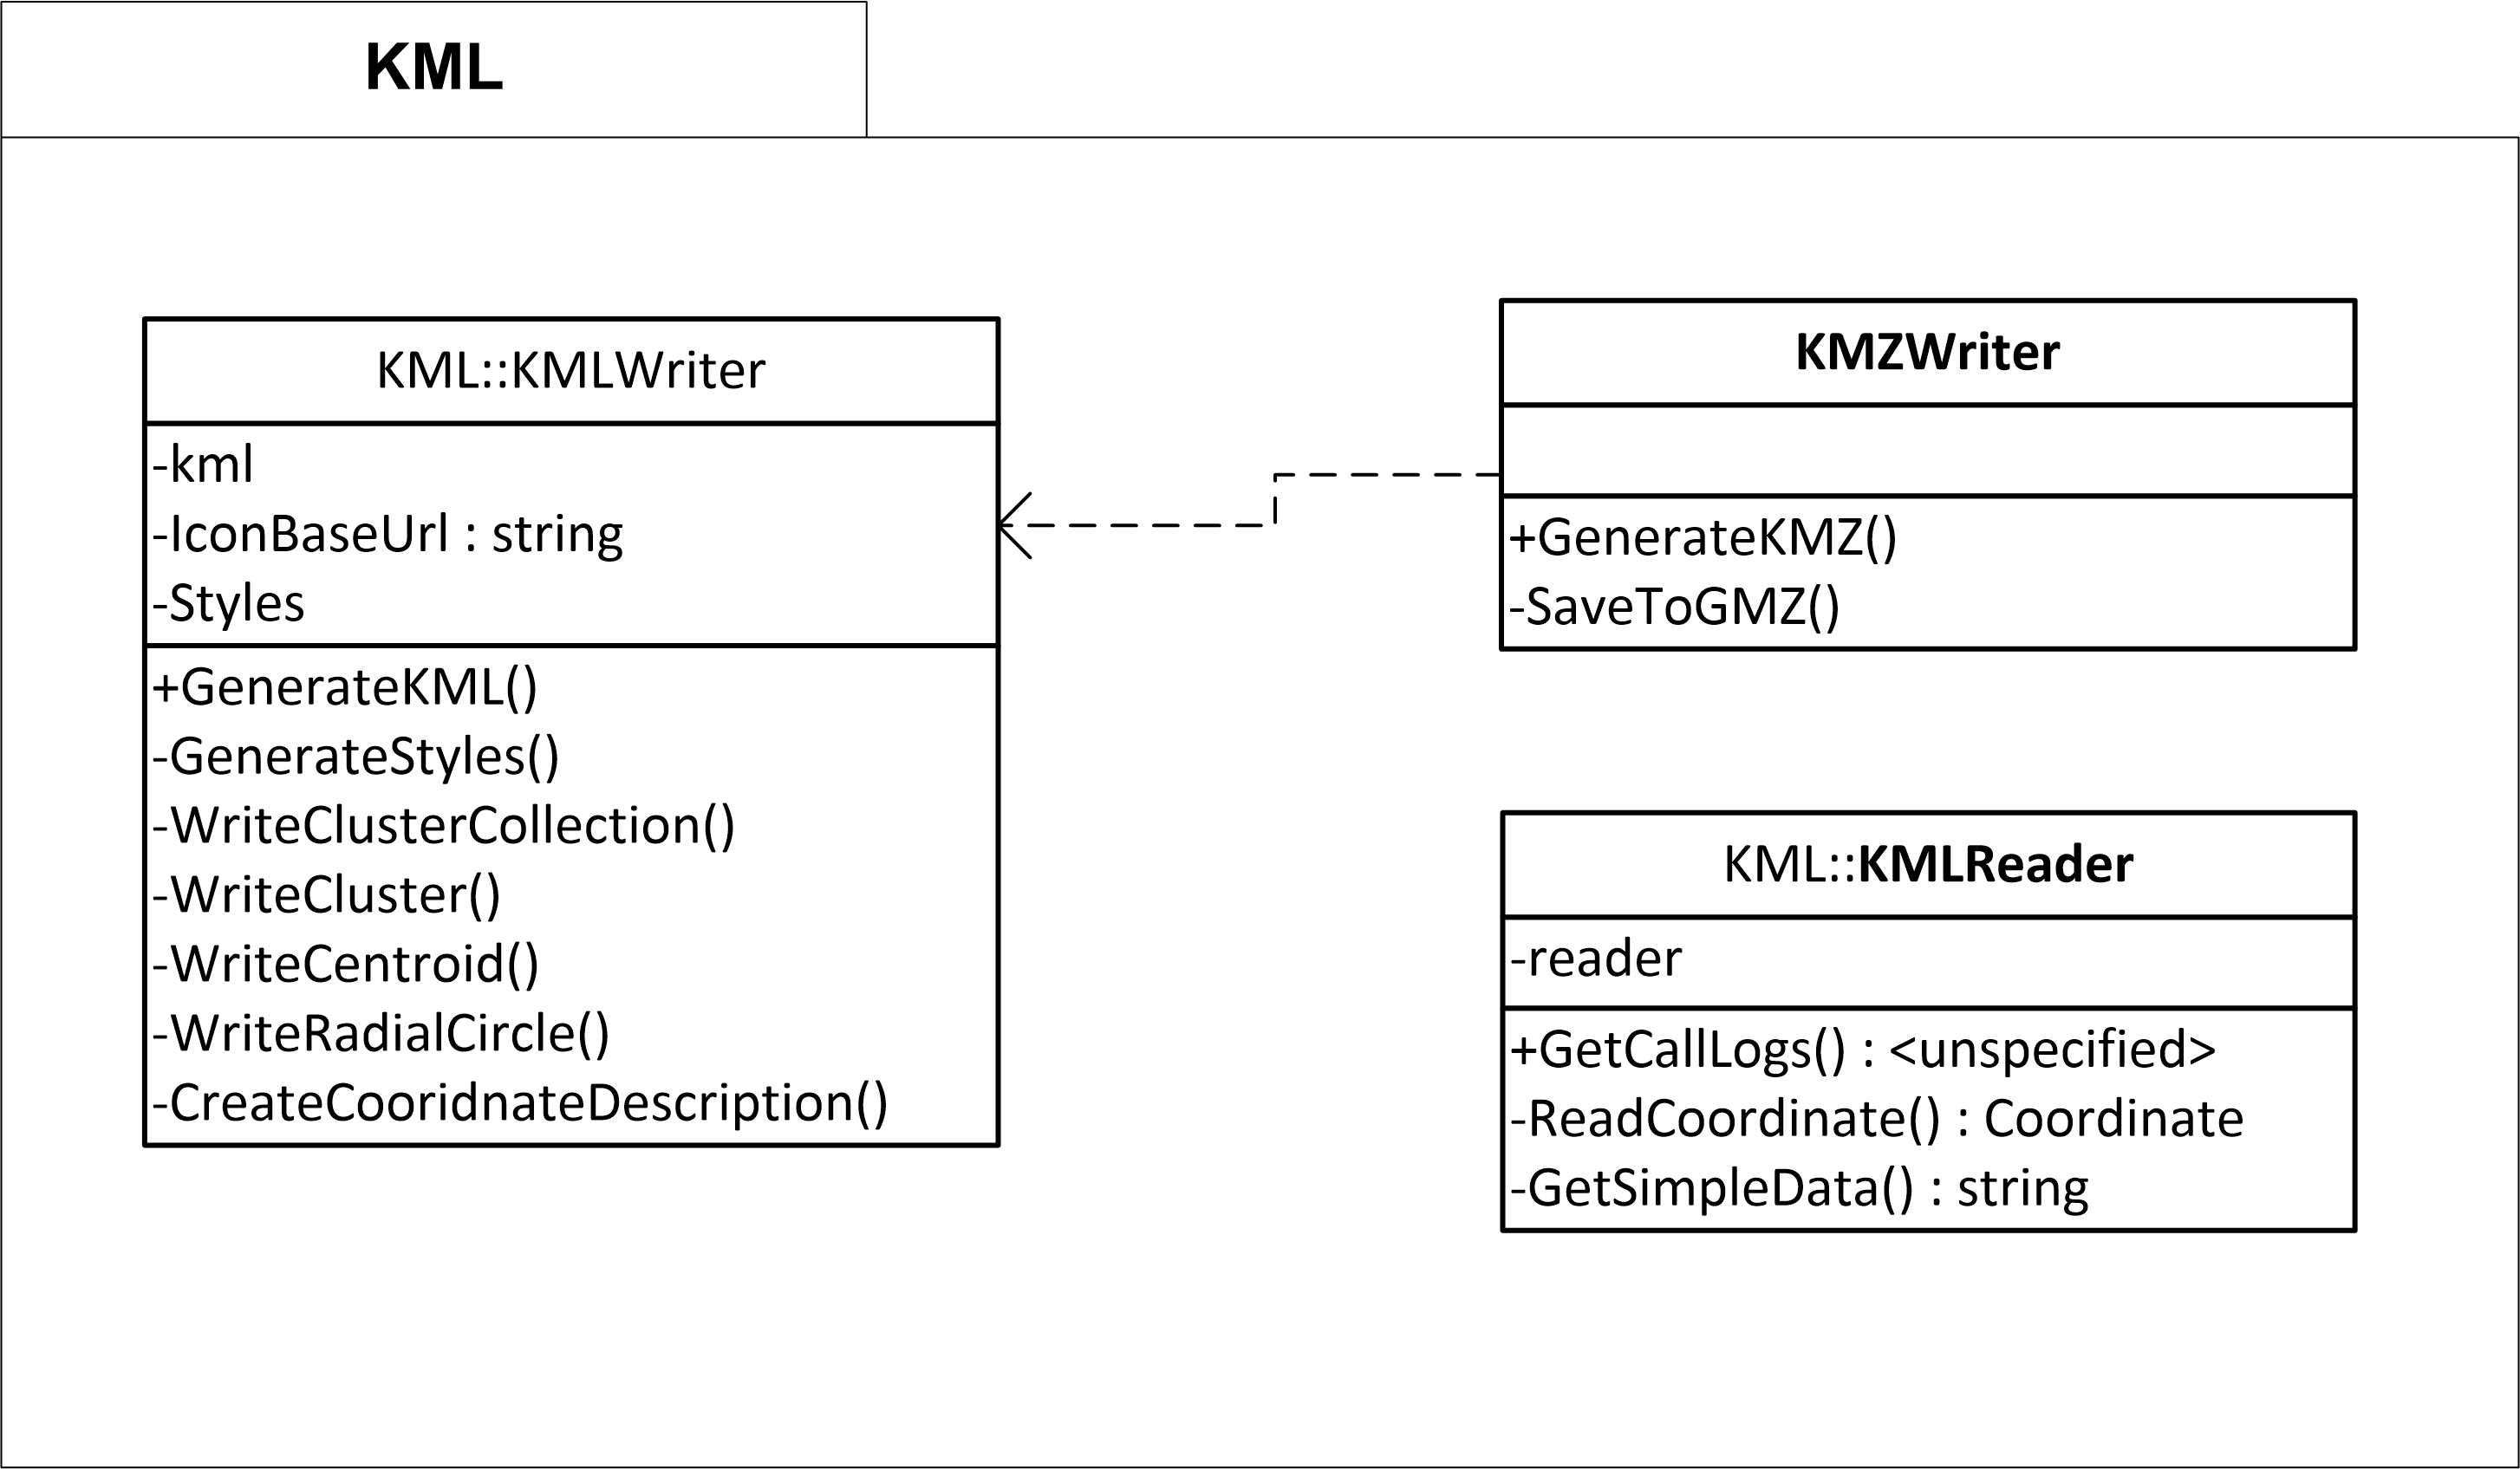
\includegraphics[scale=0.9]{chapter7/class_diagrams/kml_namespace.png}
    \caption[KML namespace class diagram]
            {KML namespace class diagram.}
    \label{fig:NSKML}
\end{figure}





% Chapter 8 - Implementation
\chapter{Implementation}

This section will focus upon the implementation of the various artefacts in 
order to successfully create the software product associated with this project.

The coding artefacts will be expressed in pseudocode, with an implementation of 
the code snippet available in the relevant appendixes. 

% C# Style
\definecolor{bluekeywords}{rgb}{0.13,0.13,1}
\definecolor{greencomments}{rgb}{0,0.5,0}
\definecolor{redstrings}{rgb}{0.9,0,0}

\lstdefinestyle{csharp}{
  language=[Sharp]C,
  showspaces=false,
  showtabs=false,
  breaklines=true,
  showstringspaces=false,
  breakatwhitespace=true,
  escapeinside={(*@}{@*)},
  commentstyle=\color{greencomments},
  keywordstyle=\color{bluekeywords}\bfseries,
  stringstyle=\color{redstrings},
  basicstyle=\ttfamily
}

 
\lstdefinestyle{pseudocode}{
  language=C,
  showspaces=false,
  showtabs=false,
  breaklines=true,
  showstringspaces=false,
  breakatwhitespace=true,
  commentstyle=\color{greencomments},
  keywordstyle=\color{bluekeywords}\bfseries,
  stringstyle=\color{redstrings},
  basicstyle=\footnotesize\ttfamily,
  morekeywords={WHILE, END, READ, CREATE, IF, NOT, DO, ELSE, FOR, WRITE, ADD,
                COMPRESS, RENAME, REMOVE, SAVE, REPEAT, UNTIL, SET, RETURN,
                CONVERT}
}


% KML File Handling
\newpage
\section{KML File Handling}

As previously mentioned figure \ref{fig:NSKML} illustrates the namespace that 
handles the reading of KML files and writing of KML and KMZ files. Within this 
section the implementation of these classes will be discussed.

\subsection{KML Reader}
The KML Reader class encapsulates an {\ttfamily XmlTextReader} object for 
which the class can be found within the {\ttfamily System.Xml} namespace. 

A KML file is a well formed XML file, and hence the reason why the 
{\ttfamily XMLTextReader} class was able to be used for the majority of the 
parsing procedure.

The main method within the file is the {\ttfamily GetCallLogs()} method, which
will return an event collection of events from the given KML file. 

If an invalid KML file is found, or no placemarks are able to be fully 
retrieved from the KML file, then the method will simply return an empty Event 
collection.

~\\
{\bfseries KMLReader::GetCallLogs()}
\lstset{style=pseudocode}
\begin{lstlisting}
  WHILE not at the end of the file
    // Obtain the Coordinate information
    READ the coordinate tag

    // Obtain the additional meta-data
    READ the device name tag
    READ the device pin tag
    READ the timestamp tag
    READ the reference tag
    READ the type tag
    READ the start rat tag
    READ the end rat tag
    READ the start mix band tag
    READ the end mix band tag
    READ the start rrc state tag

    // Create a new Event based upon the above information
    CREATE a new Event based upon the coordiante and meta-data

    // Add the parsed event
    ADD the event to the List of Events
  END WHILE

  RETURN List of Events
\end{lstlisting}
{\textsf \footnotesize File Source: src/KML/KMLReader.cs }

\subsection{KML Writer}
The KML Writer class encapsulates an {\ttfamily XmlTextWriter} object, for 
which the class can be found within the the {\ttfamily System.Xml} namespace. 

As previously mentioned, a KML file is a well formed XML file, and 
{\ttfamily XmlTextWriter} object can be used to generate a well formed KML 
file.

The main entry point for the KMLWriter class is the {\ttfamily GenerateKML()} 
method. This method is able to take a number of parameters in order to generate
a well formed KML file, and is able to perform multiple options based upon the 
given parameters.

~\\
{\bfseries KMLWriter::GenerateKML()}
\lstset{style=pseudocode}
\begin{lstlisting}
  // Create a new KML file at a given location
  CREATE new kml file

  // Insert the heatmap if given
  IF heatmap present
    ADD heatmap reference to the kml file
  END IF

  // Loop over each cluster
  FOR each cluster in clusters
    // Organise events into their clusters
    WRITE a new cluster folder

    // Loop over each event in the cluster
    FOR each event in cluster
      WRITE event to the cluster folder
    END FOR

  END FOR

  // Write noise data if available
  IF noise present
    // Organise noise events into a noise folder
    WRITE a new cluster folder

    // Loop over each noisy event
    FOR each event in noise
      WRITE event to the noise cluster folder
    END FOR

  END IF
\end{lstlisting}
{\textsf \footnotesize File Source: src/KML/KMLWriter.cs }


\subsection{KMZ Writer}
A KMZ file is a compressed KML file. One the advantages of using a KMZ file 
over a KML file is that the file is able to store images embedded directly in
itself. This is unlike a KML file, where by an image must be referenced.

The KMZWriter class has a dependency upon the KMLWriter class. The main entry 
point to the KMZWriter class is through the {\ttfamily GenerateKMZ()} method.

The method will utilise the KMLWriter class to create the KML file, and will 
then place all generated files into a compressed KMZ file.

~\\
{\bfseries KMZWriter::GenerateKMZ()}
\lstset{style=pseudocode}
\begin{lstlisting}
  // Create a new temporary working directory
  CREATE new temporary directory

  // This will create a new KML file.
  // A heatmap may also be created
  CREATE kml file and SAVE into the temporary

  // Create the temporary archive
  COMPRESS the temporary directory into an archive

  // Forms the KMZ file
  RENAME the archive extension to .KMZ

  // Remove all working files and folders
  REMOVE the temporary directory
\end{lstlisting}
{\textsf \footnotesize File Source: src/KML/KMZWriter.cs }


% Clustering - DBSCAN
\newpage
\section{DBSCAN}

The DBSCAN class provides an interface to allow for clustering of a collection 
of events. The formal description of the DBSCAN methodology and algorithm can 
be found within section \ref{sec:DBSCAN}.

For reference purposes, the basic DBSCAN algorithm is outlined below:
\begin{enumerate}
  \item Label all points as core or noise points;
  \item Eliminate noise points;
  \item Put an edge between all core points that are within {\em Eps} of each 
        other;
  \item Make each group of connected core points into a separate cluster;
  \item Assign each border point to one of the clusters of its associated core 
        points.
\end{enumerate}


\subsection{Analyse Data}
The main entry point to start the algorithm is through the use of the 
{\ttfamily Analyse()} method. The algorithm will automatically determine if 
points are noise, and if noise points are found they are removed from the 
results.

There is no limit to the number of clusters that can be generated, however 
there is a minimum number of points that are required to form a cluster. This 
value is represented by the minPts value.

~\\
{\bfseries DBSCAN::Analyse()}
\lstset{style=pseudocode}
\begin{lstlisting}
  // The "current working" cluster
  cluster = null;

  // Loop over all unvisisted events
  FOR each unvisisted event (E) in the dataset (D)
    // Prevent a revisit of the current event
    SET E as visited

    // Obtain all neighbourhood events 
    NeighbourhoodEvents = all events within the EPS distance of E

    // Ensure that there are sufficent events
    IF the total amount of NeighbourhoodEvents < MinimumPoints
      SET E as NOISE
    else
      C = next cluster
      expand all the Neighbourhood events to determine similarity
    END IF

  END FOR
\end{lstlisting}
{\textsf \footnotesize File Source: src/Clusters/DBSCAN.cs }


\subsection{Neighbourhood Search}
The {\ttfamily GetRegion()} method will return all events that are within the 
eps-neighbourhood of a given event.

~\\
{\bfseries DBSCAN::GetRegion()}
\lstset{style=pseudocode}
\begin{lstlisting}
  // The "central", given event
  Evt = given event
  
  // Loop over all known events
  FOR each event (E) in dataset (D)

    // Calculate the distance between the events
    distance = distance from E to Evt

    // Add the event if it's deemed to be a neighbour
    IF eps >= distance
      ADD E to neighbours

  END FOR
\end{lstlisting}
{\textsf \footnotesize File Source: src/Clusters/DBSCAN.cs }


\subsection{Expanding a Cluster}
The {\ttfamily ExpandCluster()} method will expand each of the event 
neighbours, and all of their neighbours. 

Ultimately, this method will deduce which events are within the given event's 
EPS neighbourhood, and hence whether or not they belong to a new cluster.

~\\
{\bfseries DBSCAN::ExpandCluster()}
\lstset{style=pseudocode}
\begin{lstlisting}
  // The given event
  GivenEvt = given event

  // Add the current event to a new cluster
  ADD event to cluster (C)

  // Get the all of evt's neighbours.
  neighbours = get all events within GivenEvts region

  // Loop over each event in GivenEvt's neighbours
  FOR each event evt in neighbours

    // Visit the evt if it has not been visited
    if evt has not been visited

      // Mark as visited
      SET evt as visited
      
      // Obtain all the events within the new region
      evtNeighbours = get all events within evts region

      // Assume all are non-noise if greater than the MinimumPoints value
      IF the total amount of NeighbourhoodEvents >= MinimumPoints

        // Merge the two neighbours lists together
        ADD evtNeighbours onto the end of neighbours
      END IF

    END IF

    // If the event doesn't belong to a cluster add to a new cluster
    IF evt does not belong to a cluster

      // Add the event to the cluster
      add evt to C
    END IF

  END FOR
\end{lstlisting}
{\textsf \footnotesize File Source: src/Clusters/DBSCAN.cs }

% Analysis
\newpage
\section{Analysis}
The Analysis aspect of the project is split up across two libraries --- 
Analysis and Analysis.Heatmap.

The first library focuses upon providing analysis for clusters on a product 
level and a week level. The library also supports multi-product and multi-week 
analysis.

The second library focuses upon providing support for generating a heatmap from
a given set of events. The library is able to change the colour scheme of the 
generated heatmap if required to.


\subsection{Analysis}
The EventAnalysis class forms the basis of all types of analysis --- referred 
to as primary analysis. The primary analysis defines operations such as the 
number of events that happened within a given cluster.

The analysis also tries to group similar events together to further highlight 
any similarities (or differences) within an intra-cluster environment, and 
across multiple weeks.

The {\ttfamily GetRatCount()} and {\ttfamily GetMixBandCount()} methods will 
return the number of events that started upon the a given RAT or MixBand 
respectfully.

Only one of the methods have been shown below, to reduce the amount of 
repeatability, as both methods have a similar implementation.

~\\
{\bfseries EventAnalysis::GetRatCount()}
\lstset{style=pseudocode}
\begin{lstlisting}
  RETURN the count of all events that started on the given start RAT.
\end{lstlisting}

~\\
As an extension to the above methods, events can be grouped by their start and 
end values. The same methods -- {\ttfamily GetRatCount()} and 
{\ttfamily GetMixBandCount()} -- support two parameters one for the start value
and one for the end value. 

Only one of the methods have been shown below, to reduce the amount of 
repeatability, as both methods have a similar implementation.

~\\
{\bfseries EventAnalysis::GetMixBandCount()}
\lstset{style=pseudocode}
\begin{lstlisting}
  RETURN the count of all events that started on the given start 
         MixBand and ended upon the given end MixBand.
\end{lstlisting}

~\\
The previous methods returned the count of events based upon the parameters 
given. In order to retrieve the actual raw events the 
{\ttfamily GroupByStartRat()} and {\ttfamily GroupByStartMixBand()} can be 
used. 

These methods require the start RAT or start MixBand respectfully. The 
pseudocode implementation of the {\ttfamily GroupByStartRat()} method is shown 
below.

~\\
{\bfseries EventAnalysis::GroupByStartRat()}
\lstset{style=pseudocode}
\begin{lstlisting}
  RETURN a key/value pair list of all events where:
            the key is the start RAT 
            the value is a list of events with the key start RAT.
\end{lstlisting}

~\\
As with the previous methods both the {\ttfamily GroupByStartEndRat()} and 
{\ttfamily GroupByStartEndMixBand()} methods support two parameters to enable
a more in depth grouping.

The pseudocode implementation of the {\ttfamily GroupByStartEndMixBand()} 
method is shown below.

~\\
{\bfseries EventAnalysis::GroupByStartEndMixBand()}
\lstset{style=pseudocode}
\begin{lstlisting}
  RETURN a key/value pair list of all events where:
            the key is the concatenation of the start MixBand and 
            end MixBand
            the value is a list of events with the given start MixBand 
            and end MixBand.
\end{lstlisting}


\subsection{Heatmap}
The Heatmap class provides various methods and functionality to be able to 
create a heat map based upon an input set of events (and their coordinates).

The design of the class is a merge between gHeat \citep{gHeat} and a bespoke 
guide written by \citeauthor{vester} \citep{vester}. The main reason for 
merging the two concepts together, was to reduce the amount of code required to
create an accurate heatmap.

The main problem with the GHeat library is that it was originally designed for 
integration with a Graphical User Interface, rather than outputting to an image 
which was the objective in this project.

The guide written by \citeauthor{vester} manages to produce a simple heatmap 
with varying colour options, however it wasn't as accurate as the gHeat 
library. By merging these two libraries together, it formed the basis of a 
powerful, and relatively simple set of heatmap classes.

The main entry point to the Heatmap is through the {\ttfamily GenerateHeatMap()}
method. This method will initialise a new blank image, and will convert each 
given event (with a coordinate) to a heatmap.

~\\
{\bfseries Heatmap::GenerateHeatMap()}
\lstset{style=pseudocode}
\begin{lstlisting}
  // Initialise a new image
  CREATE blank image

  // Convert the long/lat values to image pixels
  CREATE an intensity map
 
  // Convert the grayscale intensity map to a coloured map
  CONVERT the intensity map into a colour heat map
\end{lstlisting}

~\\
In order to create a heatmap, the original heat point is plotted onto the 
image. This forms the centroid of the heatpoint. 

Next each point of the outer circumference is generated. This is based upon the
centroid location plus a prefixed radius value multiplied by the cosine of the 
current degree of the circle.

~\\
{\bfseries Heatmap::CreateIntensityMap()}
\lstset{style=pseudocode}
\begin{lstlisting}
  // Initialise a new image
  CREATE blank image and set background to white

  // Convert coordinate points to heat points
  CONVERT Coordinate points to HeatPoints

  // Loop over all HeatPoints
  FOR each heatpoint (HP) in HeatPoints
    
    // This is the radius of the heat point 
    SET radius equal to a given value

    // This will create a circle around HP of radius.
    FOR integer (I) 1..360
      // Determine the X location
      SET x as HP.X + radius * Cos(value of I in radians)

      // Determine the Y location
      SET y = HP.Y + radius * Sin(value of I in radians)

      // Write the new heatpoint to the image 
      CREATE a new heatpoint from x and y

    END FOR

  END FOR
\end{lstlisting}


% Visualisation
\newpage
\section{Visualisation}
The final implementation stage was the visualisation of the results. To ensure 
that the visualisation was not tightly coupled to the analysis process, the 
visualisation aspect had been specifically kept as a separate entity.

The reason for this is that it allows BlackBerry to develop their own 
visualisation techniques if required, without having to change the main 
analysis processes.

\subsection{Data Management}
To ensure that the visualisation is loosely coupled with the analysis part of 
the tool, a simple data structure was required to be implemented.

As the charts were to be developed using web technologies (such as HTML, CSS 
and JavaScript), it made sense to maintain the data structures in JavaScript 
Object Notation (JSON), which is what the tool outputs.

\subsection{Charts}
In order to produce some visualisation charts, a JavaScript charting library is
required. The decision to use a well established charting library, rather than 
developing one from scratch was suggested by BlackBerry.

The requirement to develop visualisation charts was only identified as a 
`could' requirement (see section \ref{sec:could}). However due to time 
resourcing being managed well, this requirement could be fulfilled.

The charting library that was selected is call d3js. D3js is a ``JavaScript 
library for manipulating documents based on data'' \citep{d3js}. One of the 
major advantages for using d3js is that it is based upon open, standard web 
technologies (HTML, DOM, CSS and JavaScript).

This effectively means that the resulting output will be able to be displayed 
on almost any computer, without the requirement for additional software to be
installed --- other than a web standard browser.

Five charting techniques were selected to output the data, and are described in
more detail in the following subsections.


\subsubsection{Bar Chart}
The Bar Chart is one of the main points of entry to analyse the results. The 
raw data is arranged in a hierarchical structure, and this is something that 
the Bar Chart supports.

Figure \ref{fig:bar_chart_1} highlights an example bar chart from an initial 
point of view.

A user is able to ``drill down'' into the data to find specific information, by
simply clicking upon a given bar. Figure \ref{fig:bar_chart_2} highlights all 
the clusters whereby the 9800 device dropped calls upon a specific RAT. 

Clicking upon one of the bars again will drill down into the specifics of a 
cluster.

% Landscape page
\begin{landscape}
  % Center image
  \centering 
    \begin{figure}[H]
      \centering
        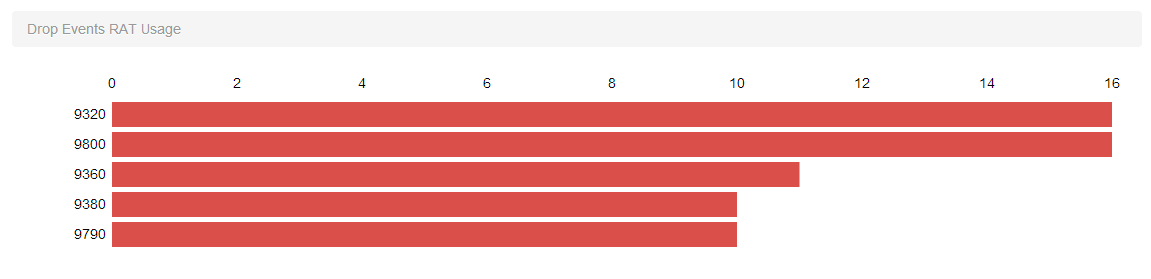
\includegraphics[scale=0.75]{chapter8/visualisation/bar_chart_1.png}
        \caption[Example Bar Chart output]
                {An Example Bar Chart output from the root node, highlighting all 
                 the various devices and their performance from a general point of 
                 view}
        \label{fig:bar_chart_1}
    \end{figure}
    ~\\
    \begin{figure}[H]
      \centering
        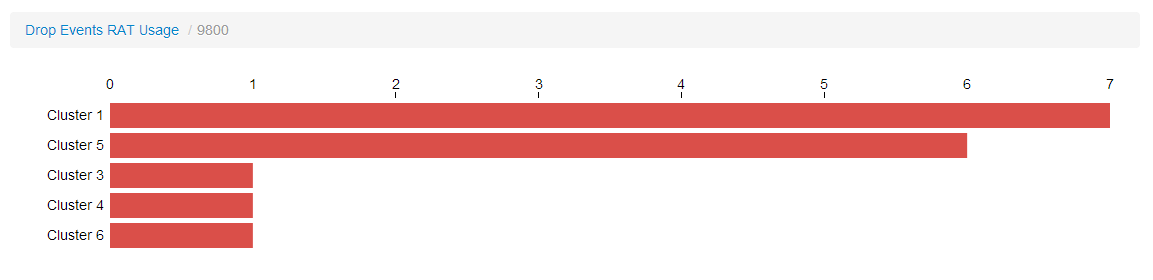
\includegraphics[scale=0.75]{chapter8/visualisation/bar_chart_2.png}
        \caption[Example Bar Chart output one node deep]
                {Example Bar Chart output one node deep --- i.e. all data that is
                 related to the 9800 device only.}
        \label{fig:bar_chart_2}
    \end{figure}
\end{landscape}


\newpage
\subsubsection{Circle Pack}
A Circle Pack diagram represents hierarchy through the use of embedded nodes. 
A Circle Pack diagram can be compared to a treemap, as it shares similar 
features however it is not as space-efficient. 

On the other hand it does reveal the overall size of each element (cluster, 
device, week, usage) more vividly in comparison to a treemap. Figure 
\ref{fig:circle_pack} illustrates an example output.

% Landscape page
\begin{landscape}
  % Center image
  \centering 
    \begin{figure}[H]
      \centering
        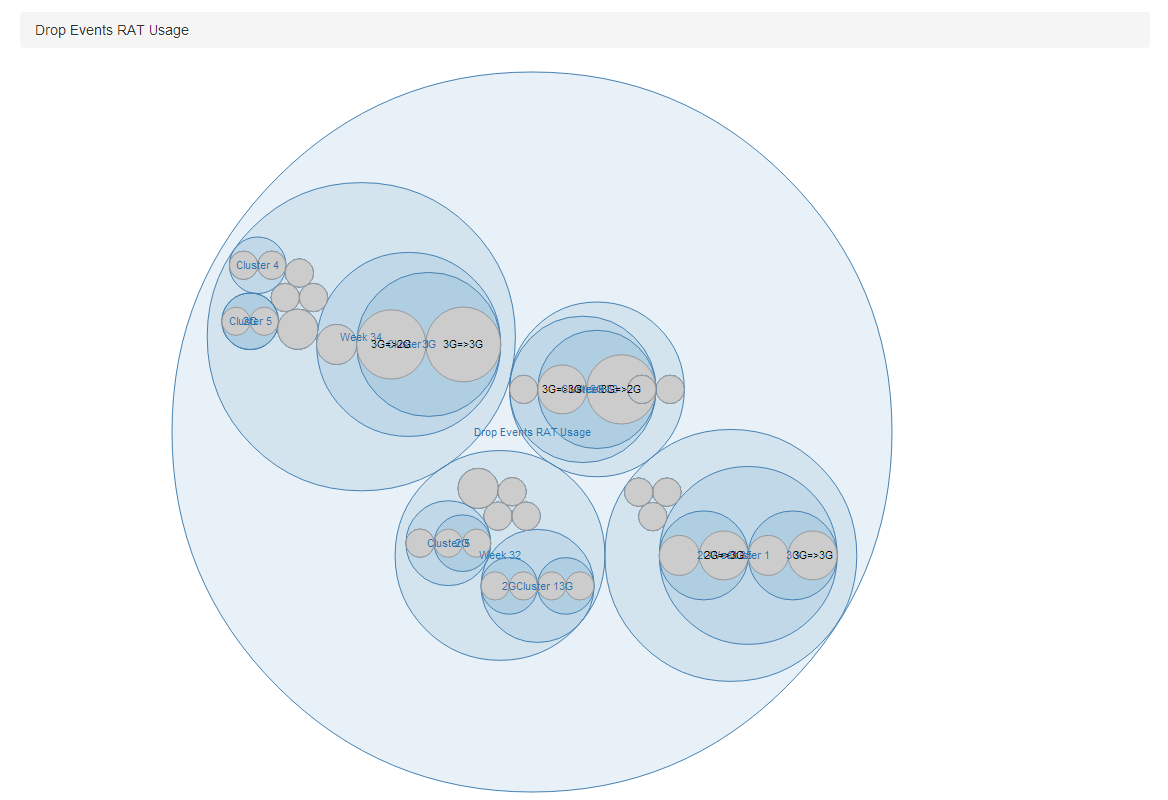
\includegraphics[scale=0.65]{chapter8/visualisation/circle_pack.png}
        \caption[Example Circle Pack output]
                {Example Circle Pack output, highlighting all the nodes. The 
               first node is the week, e.g. week 34.}
        \label{fig:circle_pack}
    \end{figure}
\end{landscape}


\newpage
\subsubsection{Dendrogram}

As with the Circle Pack diagram a dendrogram represents hierarchy through 
embedded nodes. A dendrogram is frequently used to illustrate the cluster 
arrangement formed by hierarchical clustering algorithms, although can be used 
in other ways.

Unlike the Circle Pack diagram, a dendrogram is not able to reveal the overall 
size of each element visually, and this has been shown via the raw value of 
events shown in brackets.

Figure \ref{fig:dendrogram} illustrates an example output.


% Landscape page
\begin{landscape}
  % Center image
  \centering 
    \begin{figure}[H]
      \centering
        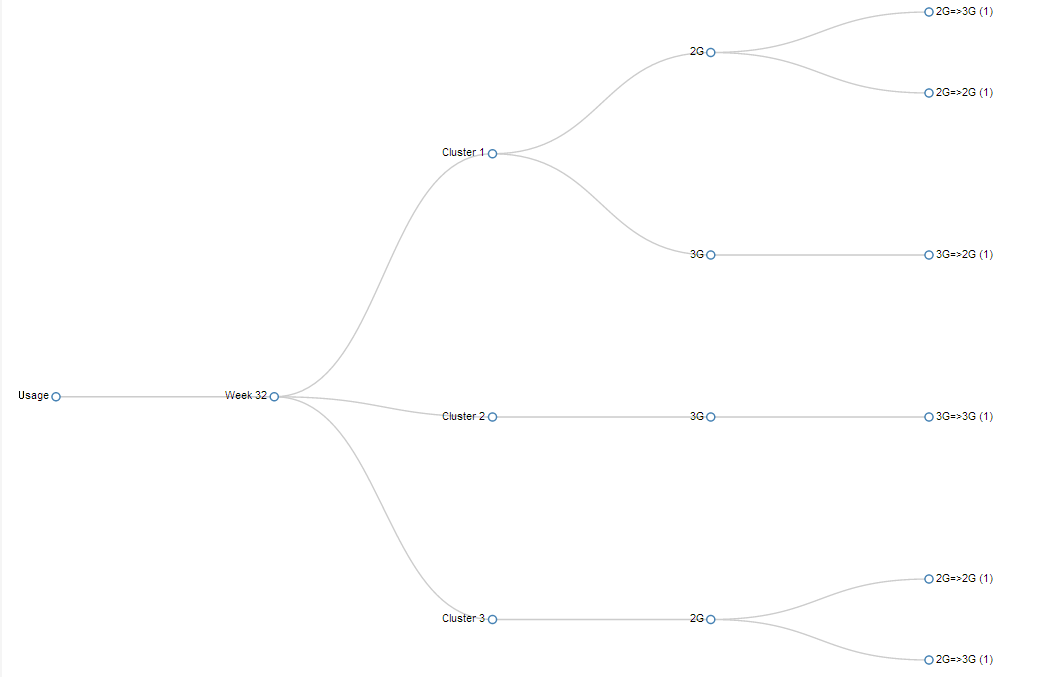
\includegraphics[scale=0.65]{chapter8/visualisation/dendrogram.png}
        \caption[Example Dendrogram output]
                {Example Dendrogram output, highlighting all the various for 
                the given week (week 32)}
        \label{fig:dendrogram}
    \end{figure}
\end{landscape}


\newpage
\subsubsection{Partition Chart}
A partition chart can thought of as an alternative to a pie chart. Although it 
looks more like a treemap, it more closely resembles the characteristics of a 
pie chart.

As with the previous charts, the partition chart supports hierarchical data. 
This allows the user to click upon a given area, and the chart will rearrange 
itself. This allows for a more bespoke, ``drilled down'' view to viewing the 
analysis.

Figure \ref{fig:partition_chart} highlights an example partition chart.

\begin{figure}[H]
  \centering
    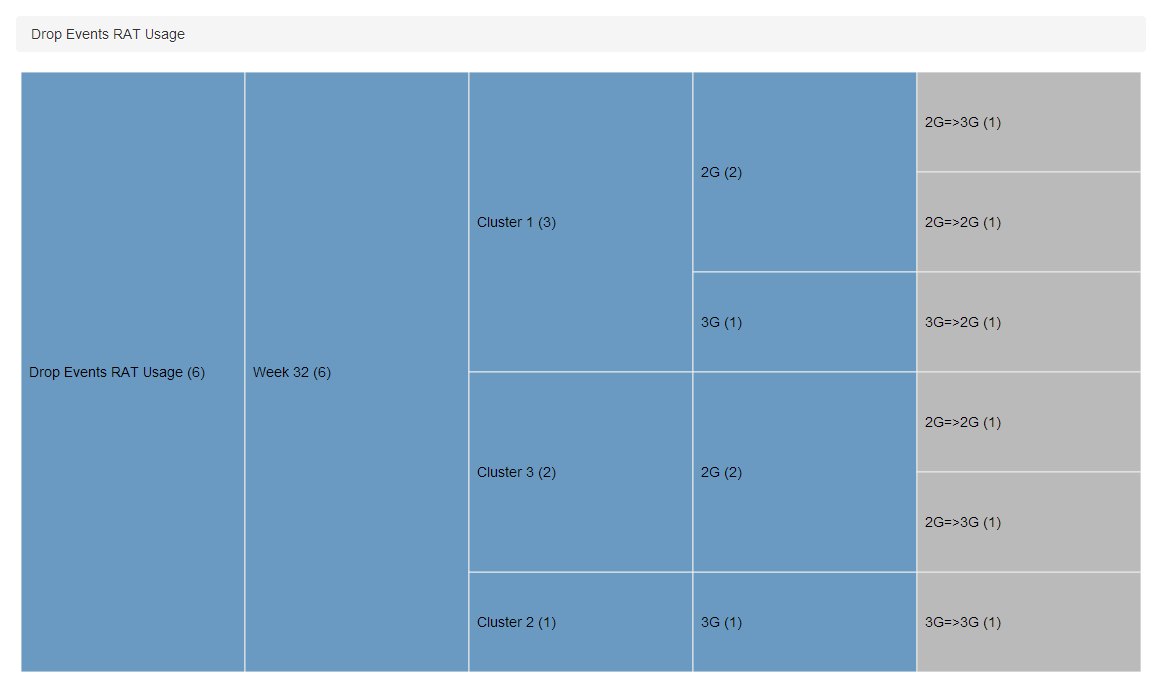
\includegraphics[scale=0.50]{chapter8/visualisation/partition.png}
    \caption[Example Partition output]
            {Example Partition output, highlighting all the nodes for the drop 
             events usage figures.}
    \label{fig:partition_chart}
\end{figure}


\newpage
\subsubsection{Treemap}
A treemap illustrates data as a set of nested rectangles. Like the partition 
chart, treemaps support hierarchical data structures.

Each square represents the total count of the events --- the larger the square 
the more events were found with the criteria. As with the partition chart, 
patterns within the data can be easily spotted. 

As a treemap grows, the efficiently of the use of space will also grow. The 
treemap implementation allows for a user to click upon a square, and it will 
rearrange itself, and as with many other charts will allow for a ``drilled 
down'' view.

Figure \ref{fig:treemap} highlights an example treemap.

\begin{figure}[H]
  \centering
    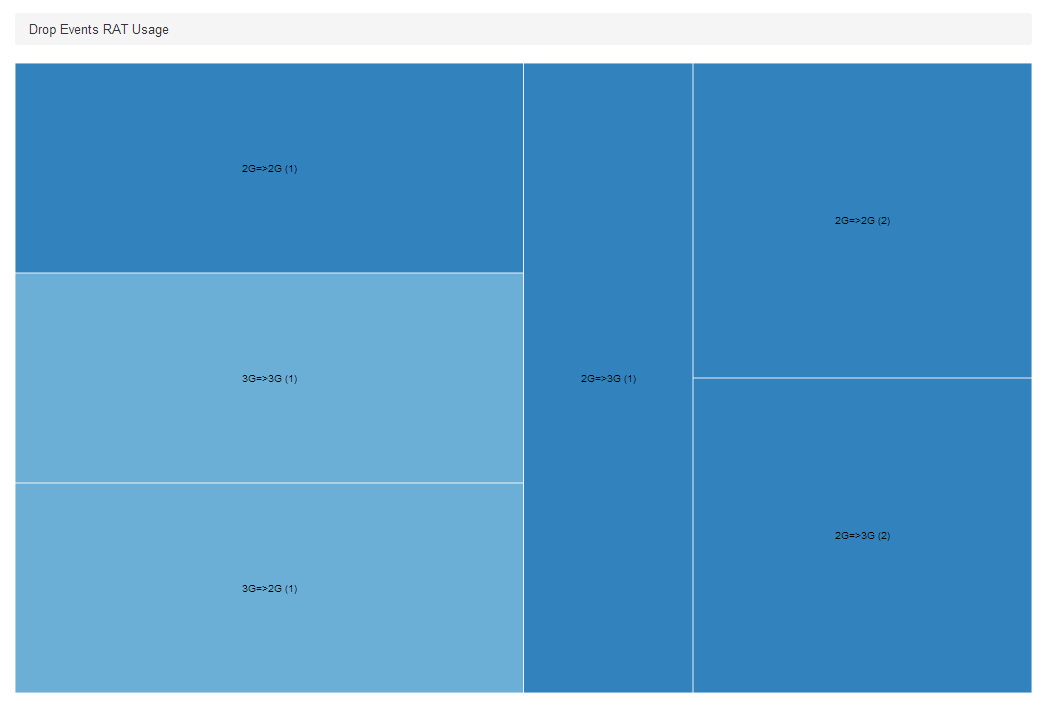
\includegraphics[scale=0.55]{chapter8/visualisation/treemap.png}
    \caption[Example Treemap output]
            {Example Treemap output, highlighting all the nodes for the drop 
             events usage figures.}
    \label{fig:treemap}
\end{figure}


% Chapter 9 - Testing
\chapter{Testing}


% Unit Test Results
\newpage
\section{Unit Testing}
\label{sec:unit_testing}

In order to test the various back end processes and methods a number of Unit 
Tests have been developed.

The classes are designed to test the underlying system, and are not able to 
test how a user interacts with the system (though a shell). The testing of the 
User Interface will be discussed within section \ref{sec:walkthroughs}.

A listing of the automated unit test classes can be found within the supplied 
software CD-ROM within the `tests' folder.

\subsection{Unit Test Implementation}

All test classes extend a main {\ttfamily Test} class. The objective of this 
test class is to ensure various constants (such as root directories) are 
available to all tests.

The Test class does not serve any other purpose.

\subsection{Test Solution Summary}
The objective behind each of the tests was to firstly ensure that a various 
stages of method calls a given variable should be equal to another variable. 

Secondly the tests ensure that not only the output was correct, but in the case
of JSON file to ensure that the output was syntactically correct. In this 
instance, if a JSON file was not syntactically correct then it would cause the 
visualisation aspect of the product to fail.

It must be noted that the visualisation web files (HTML, CSS and JavaScript) 
have not been tested via unit testing.

The reason for this is that the visualisation web files are effectively a 
framework that ``wraps around'' the JSON files --- hence why it is imperative 
that the JSON files are syntactically correct.

Table \ref{tab:test_class_summary} highlights the overall test results for each 
(unit test) class.

\begin{table}[h]
  \centering
  \begin{tabular}{|l|c|c|c|}
    \hline
    {\bfseries Test Class}   & {\bfseries Tests Passed} & 
    {\bfseries Tests Failed} & {\bfseries Tests Ignored} \\ 
    \hline
    CoordinateTest           & 5    & 0   & 0   \\ 
    CentroidTest             & 5    & 0   & 0   \\
    SphericalCoordinateTest  & 1    & 0   & 0   \\
    CoordinateCollectionTest & 5    & 0   & 0   \\
    EventCollectionTest      & 5    & 0   & 0   \\    
    KMLReaderTest            & 8    & 0   & 0   \\  
    KMLWriterTest            & 2    & 0   & 0   \\
    JSONWriterTest           & 6    & 0   & 0   \\
    DBSCANTest               & 1    & 0   & 0   \\
    DropAnalysisTest         & 6    & 0   & 0   \\ 
    FailAnalysisTest         & 6    & 0   & 0   \\ 
    WeekAnalysisTest         & 12   & 0   & 0   \\ 
    ProductAnalysisTest      & 12   & 0   & 0   \\ 
    MultiWeekAnalysisTest    & 2    & 0   & 0   \\
    MultiProductAnalysisTest & 2    & 0   & 0   \\
    \hline
  \end{tabular}
  \caption[Summary of Unit Test Results]
          {Summary of Unit Test Results}
  \label{tab:test_class_summary}
\end{table}


\subsubsection{Coordinate Test}

The {\ttfamily CoordinateTest} class tests the methods that are found 
within the Coordinate class. This class acts as a base class to other classes 
and hence will be tested multiple times.

The main objective of this unit test is to ensure that the conversion between 
decimal degrees to radians (and vice-versa) is performed correctly. It is these 
conversions that form the basis of many aspects of the tool.

Table \ref{tab:coordinate_test} highlights the Coordinate test results.

\begin{table}[h]
  \centering
  \begin{tabular}{|l|c|}
    \hline
    {\bfseries Test Method}     & {\bfseries Test Status} \\ 
    \hline
    TestToSphericalCoordinate   & {\bfseries \color{OliveGreen} PASS}   \\
    TestCoordinateInstantiation & {\bfseries \color{OliveGreen} PASS}   \\ 
    TestToString                & {\bfseries \color{OliveGreen} PASS}   \\
    TestLatitudeAsRadians       & {\bfseries \color{OliveGreen} PASS}   \\
    TestLongitudeAsRadians      & {\bfseries \color{OliveGreen} PASS}   \\
    \hline
  \end{tabular}
  \caption[Summary of the Coordinate unit test results]
          {Summary of the Coordinate unit test results}
  \label{tab:coordinate_test}
\end{table}


\subsubsection{Centroid Test}

The {\ttfamily CentroidTest} class tests the methods that are found 
within the Centroid class. This class extends the Coordinate class, and hence 
some testing will be a repeat of the {\ttfamily CoodinateTest}.

The main objective of this unit test is to ensure that the conversion between 
decimal degrees to radians (and vice-versa) is performed correctly. It will 
also ensure the radius value is being correctly used.

Table \ref{tab:centroid_test} highlights the Centroid test results.

\begin{table}[h]
  \centering
  \begin{tabular}{|l|c|}
    \hline
    {\bfseries Test Method}     & {\bfseries Test Status} \\ 
    \hline
    TestLatitudeAsRadians       & {\bfseries \color{OliveGreen} PASS} \\ 
    TestToSphericalCoordinate   & {\bfseries \color{OliveGreen} PASS} \\ 
    TestLongitudeAsRadians      & {\bfseries \color{OliveGreen} PASS} \\ 
    TestCoordinateInstantiation & {\bfseries \color{OliveGreen} PASS} \\ 
    TestToString                & {\bfseries \color{OliveGreen} PASS} \\
    \hline
  \end{tabular}
  \caption[Summary of the Centroid unit test results]
          {Summary of the Centroid unit test results}
  \label{tab:centroid_test}
\end{table}


\subsubsection{SphericalCoordinate Test}

The {\ttfamily SphericalCoordinateTest} class tests the methods that are 
found within the SphericalCoordinate class. This class extends the Coordinate 
class, and hence some testing will be a repeat of the {\ttfamily CoodinateTest}.

The main objective of this unit test is to ensure that a Spherical Coordinate 
can be formed correctly. 

This involves converting the various sub-components within a coordinate 
(longitude, latitude, elevation) into an x-axis, y-axis, and a z-axis cartesian
coordinate value.

Table \ref{tab:spherical_coordinate_test} highlights the SphericalCoordinate 
test results.

\begin{table}[h]
  \centering
  \begin{tabular}{|l|c|}
    \hline
    {\bfseries Test Method}  & {\bfseries Test Status} \\ 
    \hline
    CoordinateConversionTest & {\bfseries \color{OliveGreen} PASS} \\
    \hline
  \end{tabular}
  \caption[Summary of the SphericalCoordinate unit test results]
          {Summary of the SphericalCoordinate unit test results}
  \label{tab:spherical_coordinate_test}
\end{table}


\subsubsection{CoordinateCollection Test}

The {\ttfamily CoordinateCollectionTest} class tests the methods that are 
found within the CoordinateCollection class. This class extends the List 
class found within the {\ttfamily System. Collections.Generic} namespace.

The class largely overrides some standard features (such as adding and removing 
elements), however does feature a number of bespoke methods. The class will 
calculate the centroid of the set of coordinates every time a coordinate has 
been added or removed.

Additional non-standard methods such as splitting and merging collections will 
also be tested.

Table \ref{tab:coordinate_collection_test} highlights the CoordinateCollection 
test results.

\begin{table}[h]
  \centering
  \begin{tabular}{|l|c|}
    \hline
    {\bfseries Test Method} & {\bfseries Test Status} \\ 
    \hline
    AddCoordinateTest       & {\bfseries \color{OliveGreen} PASS}   \\ 
    SplitTest               & {\bfseries \color{OliveGreen} PASS}   \\ 
    AppendTest              & {\bfseries \color{OliveGreen} PASS}   \\ 
    UpdateCentroidTest      & {\bfseries \color{OliveGreen} PASS}   \\ 
    AddRangeTest            & {\bfseries \color{OliveGreen} PASS}   \\
    \hline
  \end{tabular}
  \caption[Summary of the CoordinateCollection unit test results]
          {Summary of the CoordinateCollection unit test results}
  \label{tab:coordinate_collection_test}
\end{table}


\subsubsection{EventCollection Test}

The {\ttfamily EventCollectionTest} class tests the methods that are found 
within the EventCollection class. This class extends the List class found
within the {\ttfamily System.Collections. Generic} namespace.

The class has a similar structure to the {\ttfamily CoordinateCollection} 
class, providing similar methods. However the main difference is the type of 
objects the hold.

Additional non-standard methods such as splitting and merging collections will 
also be tested.

Table \ref{tab:event_collection_test} highlights the EventCollection test 
results.

\begin{table}[h]
  \centering
  \begin{tabular}{|l|c|}
    \hline
    {\bfseries Test Method} & {\bfseries Test Status} \\ 
    \hline
    SplitTest               & {\bfseries \color{OliveGreen} PASS}   \\ 
    UpdateCentroidTest      & {\bfseries \color{OliveGreen} PASS}   \\ 
    AppendTest              & {\bfseries \color{OliveGreen} PASS}   \\ 
    AddEventTest            & {\bfseries \color{OliveGreen} PASS}   \\ 
    AddRangeTest            & {\bfseries \color{OliveGreen} PASS}   \\
    \hline
  \end{tabular}
  \caption[Summary of the EventCollection unit test results]
          {Summary of the EventCollection unit test results}
  \label{tab:event_collection_test}
\end{table}


\subsubsection{KMLReader Test}

The {\ttfamily KMLReaderTest} class tests the methods that are found within the
KMLReader class. This class parses a given KML file, and converts it to an
EventCollection.

In order to test the read method within this class, a number of KML files were 
given to the {\ttfamily KMLReader} class to ensure that the correct number of 
events were returned from each KML file.

Table \ref{tab:kml_reader_test} highlights the KMLReader test results.

\begin{table}[h]
  \centering
  \begin{tabular}{|l|c|}
    \hline
    {\bfseries Test Method} & {\bfseries Test Status} \\ 
    \hline
    ReadKMLFile\_L32        & {\bfseries \color{OliveGreen} PASS}   \\ 
    ReadKMLFile\_L33        & {\bfseries \color{OliveGreen} PASS}   \\ 
    ReadKMLFile\_L34        & {\bfseries \color{OliveGreen} PASS}   \\ 
    ReadKMLFile\_L35        & {\bfseries \color{OliveGreen} PASS}   \\ 
    ReadKMLFile\_T32        & {\bfseries \color{OliveGreen} PASS}   \\ 
    ReadKMLFile\_T33        & {\bfseries \color{OliveGreen} PASS}   \\ 
    ReadKMLFile\_T34        & {\bfseries \color{OliveGreen} PASS}   \\ 
    ReadKMLFile\_T35        & {\bfseries \color{OliveGreen} PASS}   \\
    \hline
  \end{tabular}
  \caption[Summary of the KMLReader unit test results]
          {Summary of the KMLReader unit test results}
  \label{tab:kml_reader_test}
\end{table}


\subsubsection{KMLWriter Test}

The {\ttfamily KMLWriterTest} class tests the methods that are found within the
KMLWriter class. This class will write a number of EventCollections and 
heatmaps to a given output KML file.

The main method has been tested against the DBSCAN output which inducing using 
the noise event collection and omitting the noise event collection data.

Table \ref{tab:kml_writer_test} highlights the KMLWriter test results.

\begin{table}[h]
  \centering
  \begin{tabular}{|l|c|}
    \hline
    {\bfseries Test Method} & {\bfseries Test Status} \\ 
    \hline
    TestGenerateKMLNoNoise  & {\bfseries \color{OliveGreen} PASS}   \\ 
    TestGenerateKMLNoise    & {\bfseries \color{OliveGreen} PASS}   \\
    \hline
  \end{tabular}
  \caption[Summary of the KMLWriter unit test results]
          {Summary of the KMLWriter unit test results}
  \label{tab:kml_writer_test}
\end{table}


\subsubsection{JSONWriter Test}

The {\ttfamily JSONWriterTest} class tests the methods that are found within 
the JSONWriter class. This class will `convert' the various internal data 
structures to the JavaScript Object Notation (JSON) equivalent.

Many of the methods found within the {\ttfamily JSONWriterTest} class will call
each other at various stages, and hence multiple tests can occur for a given 
method.

Table \ref{tab:json_writer_test} highlights the JSONWriter test results.

\begin{table}[h]
  \centering
  \begin{tabular}{|l|c|}
    \hline
    {\bfseries Test Method}      & {\bfseries Test Status} \\ 
    \hline
    TestPrettifyJSON             & {\bfseries \color{OliveGreen} PASS} \\ 
    TestCreateJSONObjectElements & {\bfseries \color{OliveGreen} PASS} \\ 
    TestCreateJSONArrayList      & {\bfseries \color{OliveGreen} PASS} \\ 
    TestCreateJSONArrayParams    & {\bfseries \color{OliveGreen} PASS} \\ 
    TestCreateKeyValue           & {\bfseries \color{OliveGreen} PASS} \\ 
    TestCreateJSONObjectKeyValue & {\bfseries \color{OliveGreen} PASS} \\
    \hline
  \end{tabular}
  \caption[Summary of the JSONWriter unit test results]
          {Summary of the JSONWriter unit test results}
  \label{tab:json_writer_test}
\end{table}


\subsubsection{DBSCAN Test}

The {\ttfamily DBSCANTest} class tests the methods that are found within the 
DBSCAN class. This class will cluster a set of events, and because of this 
only the main entry point could be tested.

The test strategy will create a number dense clusters based upon random 
geographical coordinates. The test will succeed if the algorithm manages to 
`reproduce' these clusters --- i.e. the number of expected clusters is equal to
the number of actual clusters.

Table \ref{tab:dbscan_test} highlights the DBSCAN test results.

\begin{table}[h]
  \centering
  \begin{tabular}{|l|c|}
    \hline
    {\bfseries Test Method} & {\bfseries Test Status} \\ 
    \hline
    AnalyseTest             & {\bfseries \color{OliveGreen} PASS} \\
    \hline
  \end{tabular}
  \caption[Summary of the DBSCAN unit test results]
          {Summary of the DBSCAN unit test results}
  \label{tab:dbscan_test}
\end{table}


\subsubsection{DropAnalysis Test}
The {\ttfamily DropAnalysisTest} class tests the {\ttfamily DropAnalysis} 
class. As previously mentioned, the {\ttfamily DropAnalysis} class extends the
{\ttfamily Analysis}, and testing of this class will happen at the same time of
testing the {\ttfamily DropAnalysis} class.

Table \ref{tab:drop_analysis_test} highlights the DropAnalysis test results.

\begin{table}[h]
  \centering
  \begin{tabular}{|l|c|}
    \hline
    {\bfseries Test Method}    & {\bfseries Test Status} \\ 
    \hline
    GroupByStartRatTest        & {\bfseries \color{OliveGreen} PASS}  \\ 
    GroupByStartEndMixBandTest & {\bfseries \color{OliveGreen} PASS}  \\ 
    GroupByStartEndRatTest     & {\bfseries \color{OliveGreen} PASS}  \\ 
    GroupByStartMixBandTest    & {\bfseries \color{OliveGreen} PASS}  \\ 
    GroupByStartRRCStateTest   & {\bfseries \color{OliveGreen} PASS}  \\ 
    TestAnalysisLength         & {\bfseries \color{OliveGreen} PASS}  \\
    \hline
  \end{tabular}
  \caption[Summary of the DropAnalysis unit test results]
          {Summary of the DropAnalysis unit test results}
  \label{tab:drop_analysis_test}
\end{table}


\subsubsection{FailAnalysis Test}
The {\ttfamily FailAnalysisTest} class tests the {\ttfamily FailAnalysis} 
class. As well as the {\ttfamily DropAnalysis} class the {\ttfamily FailAnalysis} 
class extends the {\ttfamily Analysis}, and testing of this class will happen 
at the same time of testing the {\ttfamily FailAnalysis} class.

Table \ref{tab:fail_analysis_test} highlights the FailAnalysis test results.

\begin{table}[h]
  \centering
  \begin{tabular}{|l|c|}
    \hline
    {\bfseries Test Method}    & {\bfseries Test Status} \\ 
    \hline
    GroupByStartRRCStateTest   & {\bfseries \color{OliveGreen} PASS}  \\ 
    GroupByStartEndMixBandTest & {\bfseries \color{OliveGreen} PASS}  \\ 
    GroupByStartMixBandTest    & {\bfseries \color{OliveGreen} PASS}  \\ 
    TestAnalysisLength         & {\bfseries \color{OliveGreen} PASS}  \\ 
    GroupByStartRatTest        & {\bfseries \color{OliveGreen} PASS}  \\ 
    GroupByStartEndRatTest     & {\bfseries \color{OliveGreen} PASS}  \\
    \hline
  \end{tabular}
  \caption[Summary of the FailAnalysis unit test results]
          {Summary of the FailAnalysis unit test results}
  \label{tab:fail_analysis_test}
\end{table}


\subsubsection{WeekAnalysis Test}

The {\ttfamily WeekAnalysisTest} class tests the methods that are found within 
the WeekAnalysis class. This class will analyse the data based upon a week 
basis.

The majority of these methods return well formed data structures, and hence the 
test strategy will look an ensuring that the correct results are returned as 
well as ensuring the data structures are correct.

Table \ref{tab:week_analysis_test} highlights the WeekAnalysis test results.

\begin{table}[h]
  \centering
  \begin{tabular}{|l|c|}
    \hline
    {\bfseries Test Method}           & {\bfseries Test Status} \\ 
    \hline
    GetFailStartEndRatFiguresTest     & {\bfseries \color{OliveGreen} PASS} \\ 
    GetDropStartRatFiguresTest        & {\bfseries \color{OliveGreen} PASS} \\ 
    GetDropStartEndRatFiguresTest     & {\bfseries \color{OliveGreen} PASS} \\ 
    GetFailStartEndMixBandFiguresTest & {\bfseries \color{OliveGreen} PASS} \\ 
    GetDropStartMixBandFiguresTest    & {\bfseries \color{OliveGreen} PASS} \\ 
    GetDropStartEndMixBandFiguresTest & {\bfseries \color{OliveGreen} PASS} \\ 
    GetFailFiguresTest                & {\bfseries \color{OliveGreen} PASS} \\ 
    GetFailStartRRCStateFiguresTest   & {\bfseries \color{OliveGreen} PASS} \\ 
    GetFailStartRatFiguresTest        & {\bfseries \color{OliveGreen} PASS} \\ 
    GetFailStartMixBandFiguresTest    & {\bfseries \color{OliveGreen} PASS} \\ 
    GetDropFiguresTest                & {\bfseries \color{OliveGreen} PASS} \\ 
    GetDropStartRRCStateFiguresTest   & {\bfseries \color{OliveGreen} PASS} \\
    \hline
  \end{tabular}
  \caption[Summary of the WeekAnalysis unit test results]
          {Summary of the WeekAnalysis unit test results}
  \label{tab:week_analysis_test}
\end{table}


\subsubsection{ProductAnalysis Test}

The {\ttfamily ProductAnalysisTest} class tests the methods that are found 
within the ProductAnalysis class. This class will analyse the data based upon a 
product basis.

As with {\ttfamily ProductAnalysis} class, the {\ttfamily ProductAnalysis} 
class return well formed data structures. The objective of this test class is 
to ensure that the correct results are returned as well as ensuring the data 
structures are correct.

Table \ref{tab:product_analysis_test} highlights the ProductAnalysis test 
results.

\begin{table}[h]
  \centering
  \begin{tabular}{|l|c|}
    \hline
    {\bfseries Test Method}           & {\bfseries Test Status} \\ 
    \hline
    GetFailStartRRCStateFiguresTest   & {\bfseries \color{OliveGreen} PASS} \\ 
    GetDropStartMixBandFiguresTest    & {\bfseries \color{OliveGreen} PASS} \\ 
    GetFailStartEndRatFiguresTest     & {\bfseries \color{OliveGreen} PASS} \\ 
    GetDropStartRatFiguresTest        & {\bfseries \color{OliveGreen} PASS} \\ 
    GetDropFiguresTest                & {\bfseries \color{OliveGreen} PASS} \\ 
    GetDropStartEndMixBandFiguresTest & {\bfseries \color{OliveGreen} PASS} \\ 
    GetFailFiguresTest                & {\bfseries \color{OliveGreen} PASS} \\ 
    GetDropStartRRCStateFiguresTest   & {\bfseries \color{OliveGreen} PASS} \\ 
    GetFailStartRatFiguresTest        & {\bfseries \color{OliveGreen} PASS} \\ 
    GetFailStartMixBandFiguresTest    & {\bfseries \color{OliveGreen} PASS} \\ 
    GetFailStartEndMixBandFiguresTest & {\bfseries \color{OliveGreen} PASS} \\ 
    GetDropStartEndRatFiguresTest     & {\bfseries \color{OliveGreen} PASS} \\
    \hline
  \end{tabular}
  \caption[Summary of the ProductAnalysis unit test results]
          {Summary of the ProductAnalysis unit test results}
  \label{tab:product_analysis_test}
\end{table}



\subsubsection{MultiWeekAnalysis Test}

The {\ttfamily MultiWeekAnalysisTest} class tests the methods that are found 
within the MultiWeekAnalysis class. This class will analyse the data based upon
a week-by-week basis.

The {\ttfamily MultiWeekAnalysis} class is an extension to the 
{\ttfamily WeekAnalysis} class. The class is able to support multiple weeks
(rather than just one). 

Many of the methods are similar to the WeekAnalysis, and to reduce 
repeatability these methods will not be tested directly. However these methods 
will be tested indirectly when formulating the results.

Table \ref{tab:multiweek_analysis_test} highlights the MultiWeekAnalysis test 
results.

\begin{table}[h]
  \centering
  \begin{tabular}{|l|c|}
    \hline
    {\bfseries Test Method} & {\bfseries Test Status} \\ 
    \hline
    AnalyseWeekTest         & {\bfseries \color{OliveGreen} PASS} \\ 
    AnalyseWeeksTest        & {\bfseries \color{OliveGreen} PASS} \\
    \hline
  \end{tabular}
  \caption[Summary of the MultiWeekAnalysis unit test results]
          {Summary of the MultiWeekAnalysis unit test results}
  \label{tab:multiweek_analysis_test}
\end{table}


\subsubsection{MultiProductAnalysis Test}

The {\ttfamily MultiProductAnalysisTest} class tests the methods that are found 
within the MultiProductAnalysis class. This class will analyse the data based 
upon a product basis.

The {\ttfamily MultiProductAnalysis} class is an extension to the 
{\ttfamily ProductAnalysis} class. The class is able to support multiple 
products across multiple weeks. 

Many of the methods are similar to the ProductAnalysis, and to reduce 
repeatability these methods will not be tested directly. However these methods 
will be tested indirectly when formulating the results.

Table \ref{tab:multiproduct_analysis_test} highlights the MultiProductAnalysis 
test results.

\begin{table}[h]
  \centering
  \begin{tabular}{|l|c|}
    \hline
    {\bfseries Test Method} & {\bfseries Test Status} \\ 
    \hline
    AnalyseWeekTest         & {\bfseries \color{OliveGreen} PASS} \\ 
    AnalyseWeeksTest        & {\bfseries \color{OliveGreen} PASS} \\
    \hline
  \end{tabular}
  \caption[Summary of the MultiProductAnalysis unit test results]
          {Summary of the MultiProductAnalysis unit test results}
  \label{tab:multiproduct_analysis_test}
\end{table}


% Walkthrough Test results
\newpage
\section{Walkthroughs}
\label{sec:walkthroughs}

The previous section (section \ref{sec:unit_testing}) discussed the automated 
test strategy. These tests assume that the data being passed around the system 
has been entered correctly.

In order to ensure that incorrect data can not interfere with the system, and 
number of `manual' walkthroughs have been proposed.

Each walkthough will ensure that the system rejects data and parameters that 
are deemed to be correct, and should inform the user of any incorrect data and 
parameters.

\newgeometry{margin=2.5cm}
\begin{landscape}
  \centering
  \setlength\LTleft{0pt}            % default: \parindent
  \setlength\LTright{0pt}           % default: \fill
  \begin{longtable}{|C{1.8cm}|l|L{2.5cm}|L{2.5cm}|L{2.5cm}|L{2.5cm}|L{2.5cm}|}
    \hline
    {\bfseries Test Number} & {\bfseries Test Data} & 
    {\bfseries Reason For Test} & {\bfseries Expected Outcome} &
    {\bfseries Actual Outcome} & {\bfseries Corrective Action Key} & 
    {\bfseries Notes} \\ 
    \hline
    \multicolumn{7}{|l|}{{\bfseries Input/Ouput File Handling}} \\
    \hline
    1                                                             &
    {\ttfamily --input="..L\_wk32\_drops.kml"}                    &
    To ensure that the tool informs the user that not enough 
    parameters have been passed to the tool.                      &
    The tool outputs the usage instructions.                      &
    As expected.                                                  &
    None.                                                         &
    None.                                                         \\
    \hline
    2                                                             &
    {\ttfamily --output=".."}                                     &
    To ensure that the tool informs the user that not enough 
    parameters have been passed to the tool.                      &
    The tool outputs the usage instructions.                      &
    As expected.                                                  &
    None.                                                         &
    None.                                                         \\
    \hline
    3                                                             &
    {\ttfamily --analysis="all"}                                  &
    To ensure that the tool informs the user that not enough 
    parameters have been passed to the tool.                      &
    The tool outputs the usage instructions.                      &
    As expected.                                                  &
    None.                                                         &
    None.                                                         \\
    \hline
    4                                                             &
    \shortstack[l]{
      {\ttfamily --input="..L\_wk32\_drops.kml"} \\
      {\ttfamily --output=".."} 
    }                                                             &
    To ensure that the tool informs the user that not enough 
    parameters have been passed to the tool.                      &
    The tool outputs the usage instructions.                      &
    As expected.                                                  &
    None.                                                         &
    None.                                                         \\
    \hline
    5                                                             &
    \shortstack[l]{
      {\ttfamily --input="..L\_wk32\_drops.kml"} \\
      {\ttfamily --analysis="all"} 
    }                                                             &
    To ensure that the tool informs the user that not enough 
    parameters have been passed to the tool.                      &
    The tool outputs the usage instructions.                      &
    As expected.                                                  &
    None.                                                         &
    None.                                                         \\
    \hline
    6                                                             &
    \shortstack[l]{
      {\ttfamily --output=".."} \\
      {\ttfamily --analysis="all"} 
    }                                                             &
    To ensure that the tool informs the user that not enough 
    parameters have been passed to the tool.                      &
    The tool outputs the usage instructions.                      &
    As expected.                                                  &
    None.                                                         &
    None.                                                         \\
    \hline
    7                                                             &
    \shortstack[l]{
      {\ttfamily --input="invalid file"} \\
      {\ttfamily --output=".."} \\
      {\ttfamily --analysis="all"} 
    }                                                             &
    To ensure that the tool informs the user that an incorrect 
    file has been passed to the tool.                             &
    The tool outputs the usage instructions.                      &
    As expected.                                                  &
    None.                                                         &
    None.                                                         \\
    \hline
    8                                                             &
    \shortstack[l]{
      {\ttfamily --input="..L\_wk32\_drops.kml"} \\
      {\ttfamily --output="invaild path"} \\
      {\ttfamily --analysis="all"} 
    }                                                             &
    To ensure that the tool informs the user that an incorrect 
    output directory has been passed to the tool.                 &
    The tool outputs the usage instructions.                      &
    As expected.                                                  &
    None.                                                         &
    None.                                                         \\
    \hline
    \multicolumn{7}{|l|}{{\bfseries Analysis Option Handling}} \\
    \hline
    9                                                             &
    \shortstack[l]{
      {\ttfamily --input="..L\_wk32\_drops.kml"} \\
      {\ttfamily --output=".."} \\
      {\ttfamily --analysis="invalid"} 
    }                                                             &
    To ensure that the tool informs the user that an incorrect 
    analysis option has been used.                                &
    The tool outputs the usage instructions.                      &
    As expected.                                                  &
    None.                                                         &
    None.                                                         \\
    \hline
    10                                                            &
    \shortstack[l]{
      {\ttfamily --input="..L\_wk32\_drops.kml"} \\
      {\ttfamily --output=".."} \\
      {\ttfamily --analysis="all"} 
    }                                                             &
    To ensure that the tool is able to analyse the given KML 
    file and output all analysis to the output directory.         &
    The tool performs a full the analysis.                        &
    As expected.                                                  &
    None.                                                         &
    None.                                                         \\
    \hline
    11                                                            &
    \shortstack[l]{
      {\ttfamily --input="..L\_wk32\_drops.kml"} \\
      {\ttfamily --output=".."} \\
      {\ttfamily --analysis="product"} 
    }                                                             &
    To ensure that the tool is able to analyse the given KML 
    file and output product analysis only to the output 
    directory.                                                    &
    The tool performs only a product analysis.                    &
    As expected.                                                  &
    None.                                                         &
    None.                                                         \\
    \hline
    12                                                            &
    \shortstack[l]{
      {\ttfamily --input="..L\_wk32\_drops.kml"} \\
      {\ttfamily --output=".."} \\
      {\ttfamily --analysis="week"} 
    }                                                             &
    To ensure that the tool is able to analyse the given KML 
    file and output week analysis only to the output 
    directory.                                                    &
    The tool performs only a week analysis.                       &
    As expected.                                                  &
    None.                                                         &
    None.                                                         \\
    \hline
    13                                                            &
    \shortstack[l]{
      {\ttfamily --input="./kml\_input\_folder"} \\
      {\ttfamily --output=".."} \\
      {\ttfamily --analysis="all"} 
    }                                                             &
    To ensure that the tool is able to analyse the given input 
    directory and output all analysis to the output directory.    &
    The tool performs a full the analysis.                        &
    As expected.                                                  &
    None.                                                         &
    None.                                                         \\
    \hline
    14                                                            &
    \shortstack[l]{
      {\ttfamily --input="./kml\_input\_folder"} \\
      {\ttfamily --output=".."} \\
      {\ttfamily --analysis="product"} 
    }                                                             &
    To ensure that the tool is able to analyse the given input 
    directory and output product analysis only to the output 
    directory.                                                    &
    The tool performs only a product analysis.                    &
    As expected.                                                  &
    None.                                                         &
    None.                                                         \\
    \hline
    15                                                            &
    \shortstack[l]{
      {\ttfamily --input="./kml\_input\_folder"} \\
      {\ttfamily --output=".."} \\
      {\ttfamily --analysis="week"} 
    }                                                             &
    To ensure that the tool is able to analyse the given input 
    directory and output week analysis only to the output 
    directory.                                                    &
    The tool performs only a week analysis.                       &
    As expected.                                                  &
    None.                                                         &
    None.                                                         \\
    \hline
  \end{longtable}
\end{landscape}


% Chapter 10 - Maintenance
\chapter{Maintenance}

\section{Work in Progress}
\section{Future Enhancements}

% Chapter 11 - Evaluation
\chapter{Evaluation}
\label{cha:evaluation}

Throughout this project there have been two deliverables --- the software 
product and the project itself.

The evaluation will evaluate both the product and the project as separate 
elements, as well as providing an industry and personal reflection.

% Product Evaluation
\newpage
\section{Product Evaluation}
\label{sec:product_evaluation}

The Cluster Analysis Tool that was developed as part of this final year project
could be regarded as a success. Although there are a number of improvements and
extensions that could be made, it is clear that when comparing the final 
product to the original user requirements set by BlackBerry (section 
\ref{sec:userrequirements}), there are little differences.

The Cluster Analysis Tool successfully parses a KML file and converts each of 
the given placemarks into Call Events. All call events can be clustered into 
various clusters by utilising an implementation of the DBSCAN algorithm.

Once the clustering process has been completed, the tool is able to provide a 
number of analysis options, and is ultimately output the analysis in various 
graphical formats.

As well a producing graphical outputs, the tool is also able to output to a 
KML file. Once opened in Google Earth, the KML file is able to display the 
various clusters, along with the radius around the centroid of each cluster. 

Each event is able to be clicked upon for more information, as well as allowing
the end user to ``overlay'' multiple KML files to view multiple weeks and/or 
multiple products.

Although a Graphical User Interface could have been developed, it was decided 
to keep the tool as a command line tool. This allows for a simple integration
with current internal BlackBerry systems, and it allows for an automated 
approach to utilising the tool (as well as a manual approach).

As it stands the product does meet all of the original requirements, however 
there are a number of improvements that could be made to further better the 
product.

Firstly the test route could shown within the output KML file. This would allow
for each event to be highlighted upon the route. In order for this to be 
achieved, the route would have to be added to the original KML file. 

Adding the route would not change the analysis or clustering processes, however
it would improve the overall link between the route and the call events.

Additionally, an overall area percentage figure could be introduced. This 
percentage would be the number of drops multiplied by the area coverage for a
given geographical coordinate. Typically the area coverage is 5m$^2$ (25m). 

This would mean that if there were 20 events within a 1KM radius, then the 
total area percentage representing events would be calculated as:

\begin{center}
  $ \large \frac{20 \times 0.25}{\pi \times 1^2} \times 100 = 15.9\% $
\end{center}

Effectively, this means that 15.9\% of the given cluster (in terms of area) 
represents call events.

~\\

Overall, the product meets the required specifications of this project. More 
specifically, the product has managed to ensure that the ``Must'' and 
``Should'' requirements are completed with some of the ``Could'' requirements
completed as well.


% Project Evaluation
\newpage
\section{Project Evaluation}
\label{sec:project_evaluation}

In total, forty-four weeks was formally set a side to complete this project.
However, I have managed to complete the project fully in thirty-nine weeks. It 
is clearly obvious that the time management skills used throughout this project 
helped to deliver the project well within the allocated time.

At every major stage (such as research, analysis, implementation etc) a high 
quality piece of work has been initially produced, refined and improved through
client, supervisor and examiner feedback.

The largest amount of time spent was compiling the research section. Overall 
three major areas of computing --- mobile networks, clustering and 
visualisation techniques --- were managed to be researched in a great amount 
of depth. It is this additional understanding that was able to be applied in 
some of the key sections found later on, such as the design and implementation 
stages.

Development time was considerably lower than what I had originally planned for.
There are several reason for this. Firstly due to the increased time that I had
managed to obtain through starting the project early, I was able to spend more 
time upon the Research and Design sections. This allowed for a more, rounded
well thought out approach to the project .

Secondly the design section of the project was carried out with careful 
consideration. This was to ensure that all aspects were covered, to ensure that
the best possible design and implementation could have been produced.

Finally, the development strategy was to use an incremental evolutionary 
prototype approach. This is a hybrid of the incremental strategy and the 
evolutionary strategy. The reason for this is that it allowed for each MoSCoW 
objective to be developed independently, and to be able to receive direct 
feedback from BlackBerry.

The modules that were developed help to keep the overall testing time down. The
reason for this is that each module could be tested independently, and did not
require any dependencies from other modules. Furthermore, testing was conducted
as development occurred. This highlighted a large percentage of bugs, and were 
fixed immediately.

To ensure the project was on track various meetings took place throughout the 
year. 

A weekly project meeting in the style of a `quality circle' was attended in by 
myself, my supervisor and other group peers. These meetings provided an 
opportunity for various topics of discussion to occur. The topics included new 
ideas that could be integrated into the product or project, as well as 
providing feedback upon current ideas. 

A bi-weekly product meeting was conduced via a conference call between myself 
and Anup who is the Call Performance Team Leader for BlackBerry.

Anup would provide feedback upon any development work that was conducted, as 
well as discussing any future functionality. These calls proved to be useful, 
as it allowed for the bridge between an academic project and an industry 
product to take place.

As part of the integration strategy, I was asked to conduct a presentation upon
the project as whole to BlackBerry. This allowed for various research topics to
be presented, as well as the design principles behind the software product to 
be highlighted. 

As part of the mid-term review of the project, a poster was used to consolidate
all the research and design ideas obtained up to that point. The poster was 
presented to the various members of academic staff, research staff as well as 
other peers. This allowed for valuable feedback to be obtained from a wide 
audience, as well discussing current progress and future expected progress.

The aims of this project were to demonstrate that is is possible to cluster 
mobile call coverage figures, as well as analysing these figures to provide an 
in depth understanding of call performance. After completing this project and 
gaining valuable feedback from BlackBerry, it is clearly evident that the 
project can be classified as a success.

% Industry Reflection
\newpage
\section{Industry Reflection}
\label{sec:industry_reflection}

\begin{quote}
The Cluster Analysis Tool is a project executed by Luke as part of his final 
year project. The tool is an extension to an in-house project that was started
by Luke during his placement (Call Performance Analysis and Reporting System 
--- CPARS).

CPARS is able analyse various test routes and the results of the tests upon a 
large scale, however it is unable to provide analysis upon a geographical 
level.

The Cluster Analysis Tool is able to provide this level of geographical 
analysis as well as being able to automate the performance analysis activities 
within BlackBerry.

The tool has now been delivered to BlackBerry and meets many of the 
requirements that were initially defined. 
 
The tool allows BlackBerry to analyse the field performance of its devices by 
clustering events (drops and fails) that occur within a close geographical 
proximity of each other.

The tool produces valuable features, to which when integrated with CPARS, will
help test engineers to improve the analysis and understanding of these events. 

The tool has immense potential and it was only due to time constraints that 
caused certain requirements to be left out of delivery --- e.g. the ability to
detect differences of velocity between two data sets.
 
Our team is very impressed and grateful to Luke for the delivery of tool.
\end{quote}

\begin{flushright}
Anup Vijay \\
Call Performance Team Leader \\
Monday, 22$^n$$^d$ April 2013
\end{flushright}

% Personal Reflection
\newpage
\section{Personal Reflection}
\label{sec:personal_reflection}

The original proposal for this project was put forward by Anup (Call 
Performance Team Leader, BlackBerry) during the final month of my industrial 
placement. 

I was particularity interested in this project, as it was a follow on project 
from some of the work that I had completed upon placement.

Initially I was aware that I would have to produce some form of algorithm that
would cluster the calls in to groups. I was also aware that in some form or 
another I would have to define exactly what a cluster is, and how the algorithm 
could `detect' a cluster.

For me this posed an interesting problem, to which I would be able to solve 
though using standard computing practises. 

As a Software Engineer, I have to actively embrace the principles of 
engineering in order to analyse, design, develop and test software systems. 
This problem had to opportunity to test all of these key areas.

I found the research aspect of the problem incredibly interesting. Not only was
it technically based, it was also heavily philosophically based. The majority 
of the background research was obtained when I was upon placement, with further 
academic references added in over the due course of the project.

However I did found it interesting that the cluster analysis research was just 
as philosophical as it was technical. From a technical point of view there were
little arguments and deviations. However this was quite the opposite when some 
of the philosophical aspects of cluster analysis were discovered.

As an example, I found that the definition of a cluster was not only ambiguous,
it also had a philosophical nature. One individual could state that a dataset 
had a certain number of clusters, where as another individual could state that
figure to be something completely different.

These differences in opinions could have been obtained from different 
understandings of the original data set, to even the visual representation of 
the data set. 

I found out that it was simply the definition of a cluster that was the hardest
aspect of the field, not what I had originally expected which was the 
development and implementation of the algorithm.

I found the majority of the development straight forward, which was down to a 
number of major aspects. 

Firstly, BlackBerry activity engaged in the analysis and development stages of 
the project. This ultimately ensured that the end product was correct, and that
it met all of the system requirements.

Ideas were constantly bounced back between myself and Anup to try solve any 
minor problems that might have occurred during development. 

As previously mentioned, it also allowed for an industry quality circle to be 
formed, which ensured that the quality was there, and that the objectives were
always being met.

Secondly as I had an understanding of the mobile network, and some of the 
analysis activities that took place within BlackBerry, I was able to utilise 
my previous placement experience to leverage any work. 

An example of this can be found in which the way the analysis is shown. Call 
drop events are shown as red, and setup failure events are show as yellow. It 
is this common theme, that allows BlackBerry test engineers to instantly 
recognise what the analysis is trying to tell them.

Finally, as previously mentioned this project was a follow on project from my 
placement year. This fundamentally meant that I was able to start earlier. 

It was pushing the start time of the project forward, that enabled me to ensure 
that all research was conducted thoroughly, and that the requirements had been
correctly analysed and mapped to development targets.

It also provided some additional ``breathing room'' when other university 
commitments had to take priority.

~\\

I can certainly say that I have thoroughly enjoyed this project, partially the 
academic research side of the project. Consequently, my academic research 
skills have managed to improve substantially. 

I am also able to state that I have been able to re-enforce a second 
programming language in such a way that I could classify myself as an advanced 
user. 

As well as re-enforcing known development technologies, I have also been able
to learn new technologies. 

It is the combination of new skills learnt and the further improvement of 
existing skills that I will be able to cherish for future projects.

% Chapter 12 - Conclusion
\chapter{Conclusion}
\label{cha:conclusion}

During this report it was shown that it is possible to cluster a set of call 
usage data to obtain some useful analysis. Although the clustering is only 
completed upon one set of attributes within the dataset, the additional 
analysis manages to highlight similarities and differences between each 
cluster.

Clustering call logs is probably nothing new (although this is unconfirmed due
to the secrecy of the industry). However trying to highlight the similarities 
and differences between devices performing well and badly is a common interest 
within the industry.

The research highlighted that there are a number of common techniques that can 
be applied to a set of data to distinguish a set of clusters. Each of these 
techniques has various advantages and disadvantages over their counter 
techniques.

Once the analysis process has completed, the results are represented as 
numerous in-memory data structures (before being saved to disk). This allows 
for logical access to the specifics and generalisations of the analysis 
relatively simply.

Each class was tested utilising Unit Testing, with the final complete system 
being testing via a basic smoke test. Dynamic testing of the system occurred 
upon the fly as the tool was being developed, which enabled the overall testing
time to decrease.

This project has shown that a Cluster Analysis Tool can be successfully 
implemented utilising standard computing knowledge and principles. This is 
despite the fact that the data that the tool clustered and analysed could be 
regarded as `non-standard'.

Due to the nature of the project, it does obviously rely upon a fixed data 
structure, however it is possible to change and extend the data structure in 
the future should there be a requirement to do so.

Although this project has focused on the clustering and analysis of call data, 
the methodology used throughout this project has demonstrated that a large 
problem can be split up into smaller, more manageable tasks.




% Citations
\bibliographystyle{plainnat}
\bibliography{references/citations}
\end{document}